\documentclass[a4paper, 11pt, twoside]{report}
\usepackage[utf8]{inputenc}
\usepackage{csquotes}
\usepackage[hidelinks]{hyperref}
\usepackage[left=2.5cm,right=2.5cm,top=2.5cm,bottom=3.0cm]{geometry}
\setlength{\headheight}{13.6pt}
\hbadness=10000
\usepackage{graphicx}
\usepackage[english]{babel}
\usepackage[justification=centering]{caption}
\usepackage[T1]{fontenc}
\usepackage{lastpage}
\usepackage{hyperref}
%Custom commands
\newcommand{\chref}[1]{\ref{#1}}
\newcommand{\secref}[1]{\ref{#1}}
\newcommand{\subsecref}[1]{\ref{#1}}
\newcommand{\note}[1]{\textcolor{violet}{#1}}
\newcommand{\power}{$P_{\text{density}}$ }
\newcommand{\Cd}{$^{109}Cd$ }
\newcommand{\Sr}{$^{90}Sr$ }
\newcommand{\Fe}{$^{55}Fe$ }
\newcommand{\noise}{$\sigma_\text{V}$ }
\newcommand{\thr}{$V_\text{thr}$ }
\newcommand{\toa}{\textit{ToA}}
\newcommand{\dtoa}{$\Delta_{TOA}$ }
\newcommand{\sigdtoa}{$\sigma_{\Delta_{TOA}}$ }
\newcommand{\sigdut}{$\sigma_{\text{DUT}}$ }
\newcommand{\sigmcpzero}{$\sigma_{\text{MCP0}}$ }
\newcommand{\sigmcpone}{$\sigma_{\text{MCP1}}$ }
\newcommand{\dtoaid}{$\Delta_{TOA,i, d}$ }
\newcommand{\sigdtoad}{$\sigma_{\Delta_{TOA,d}}$ } 

\newcommand{\vth}{$V_{\it{th}}$}
\newcommand{\pdensity}{$P_{\it{density}}$}
\newcommand{\maxflu}{$1 \times 10^{16}$ n$_{\text{eq}}$/cm$^2$}
\newcommand{\flu}{n$_{\text{eq}}$/cm$^2$}

\usepackage{enumerate}
\usepackage{lmodern}
\usepackage{float}
\usepackage{amsmath, amssymb, esint}
\usepackage{array}
\usepackage[dvipsnames]{xcolor}
\usepackage{multirow}
\usepackage{subcaption}
\usepackage{dsfont}
\usepackage{tensor}
\usepackage{fancyhdr}
\usepackage{listings}
\usepackage{dsfont}
\usepackage{siunitx}
\usepackage{tikz-feynman}
\usepackage{physics}
\usepackage[sorting=none]{biblatex}
\addbibresource{./bib.bib}
\usepackage{changepage}
\usepackage[acronyms]{glossaries}
\tikzfeynmanset{compat=1.1.0}
\sisetup{output-exponent-marker=\textsc{e}, bracket-negative-numbers, open-bracket={\text{-}}, close-bracket={}}
\pagestyle{fancy}
\fancyhead[LE,RO]{\leftmark}
\fancyhead[RO,LE]{}
\lfoot{}
\cfoot{\thepage}
\rfoot{}
\renewcommand{\headrulewidth}{0.1pt}
\renewcommand{\footrulewidth}{0.1pt}
\newcommand{\HRule}[1]{\rule{\linewidth}{#1}} 	% Horizontal rule
\makeatletter							% Title
\def\printtitle{%						
    {\centering \@title\par}}
\makeatother									

\makeatletter							% Author
\def\printauthor{%				
    {\centering \large \@author}}				
\makeatother							


\begin{document}

\begin{titlepage}
	\centering % Centre everything on the title page	
	\scshape % Use small caps for all text on the title page
	\vspace*{\baselineskip} % White space at the top of the page
	
	%------------------------------------------------
	%	Title
	%------------------------------------------------
	
	\rule{\textwidth}{1.6pt}\vspace*{-\baselineskip}\vspace*{2pt} % Thick horizontal rule
	\rule{\textwidth}{0.4pt} % Thin horizontal rule
	
	\vspace{0.75\baselineskip} % Whitespace above the title
	
	{\LARGE The FASER Preshower upgrade:\\} 
	\vspace{0.25\baselineskip}
	{\Large A high spatial resolution W-Si preshower detector enabling sensitivity to Long-Lived Particle decays into photons\\}
	% {\Large  through the development and assembly of a Monolithic Silicon Pixel Detector.} % Title
	
	\vspace{0.75\baselineskip} % Whitespace below the title
	
	\rule{\textwidth}{0.4pt}\vspace*{-\baselineskip}\vspace{3.2pt} % Thin horizontal rule
	\rule{\textwidth}{1.6pt} % Thick horizontal rule
	
	\vspace{2\baselineskip} % Whitespace after the title block
	
	%------------------------------------------------
	%	Subtitle
	%------------------------------------------------
	
	\textit{2021 - 2025}
	
	\vspace*{0.5\baselineskip} % Whitespace under the subtitle
	
	%------------------------------------------------
	%	Editor(s)
	%------------------------------------------------
	
	\begin{center}  
\includegraphics[width=7cm]{UniGe_Logo}  \end{center}
	
	\vspace*{0.5\baselineskip}
	
	Written by
	
	\vspace{0.5\baselineskip} % Whitespace before the editors
	
	{\scshape\large Théo Moretti} % Editor list

	\vspace{2\baselineskip} % Whitespace below the editor list
	
	\textit{\large Université de Genève, Suisse \\
			Section de Physique - Département de Physique Nucléaire et Corpusculaire \\}
			\texttt{theo.moretti@unige.ch} \\ % Editor affiliation
	
	\vspace{2\baselineskip} % Whitespace between editor names and publisher logo

Supervised by Professor Giuseppe Iacobucci
	
	
	\vspace{0.3\baselineskip} % Whitespace under the publisher logo
	
	

\end{titlepage}

				
\newpage
\tableofcontents
\thispagestyle{empty}
\newpage
\setcounter{page}{1}

\chapter*{Acknowledgements}


% TODO ALL: Choose between impersonal or personal "we" pronouns and correct it throughout the full thesis 
% TODO ALL: Decide how to write the left panel right panel if in bold, write in text or just leave as parenthesis before the explanation or at the end of the explanation

\vspace{15mm}


\hspace{120mm}

\chapter{Introduction}

In the quiet observation of the reality surrounding us, the attention of the human eye is often captured by the recognition of patterns, some structures, regularities or even symmetries repeating themselves across space and time. In Physics, symmetries are not only just an esthetical feature of Nature but is more of a guiding principle that underlies the formulation of physics laws. Over time, the study of such symmetries have shaped the way physicist have described the fundamental interaction governing the Universe. One of the multiple consequences of this perspective is known as Emmy Noether's first theorem she enunciated in 1915. In its general form, the theorem states that: 
\begin{center}
  \textit{'To every differentiable symmetry generated by local actions, there corresponds a conserved current'}
\end{center}

This statement is deeply connected to a more fundamental principle and requirement for any physical law: covariance. Noether's theorem provides a mathematical framework for expressing conservation laws through continuity equations. Initially applied to the explanation of conservation of energy, momentum and angular momentum through the symmetries of space and time in classical physics, it is now a pillar of modern theoretical physics, influencing fields such as Quantum Field Theory or General Relativity. \\
As of now, the description of the fundamental constituents of matter is performed by the Standard Model of particle physics, based itself on the rigorous mathematical framework of Quantum Field Theory. 
The Standard Model was developed in the early 1970s and is yet the best description of the fundamental constituents of matter, the particles, and the fundamental forces governing them. It has not only allowed physicist to perform precise predictions on a wide variety of phenomena but also to give explanation to almost all the experimental results obtained until now. \\ 

The matter particles all share one property which is their spin of one-half, they are hence called fermions. These later can further be divided into two subgroups, the quarks and the leptons, themselves divided into three generations depending on their stability. The first generation is associated with the lighter and thus more stable particles while the two other generations are associated to heavier and thus less stable particles. For this reason, the particles of the first generation are the ones we identify as components of the stable matter observed in the Universe.
There are four know fundamental forces acting on the particles, but only three of them are described by the Standard Model, the outlier being the gravitational force. Each of the forces is associated to the exchange of force-carriers particles which all have an integer value for their spin, they are hence called bosons. One last boson completes the model, the Higgs boson, responsible for the mass of the particles. \\ \clearpage

\begin{figure}[h]
	\centering
 	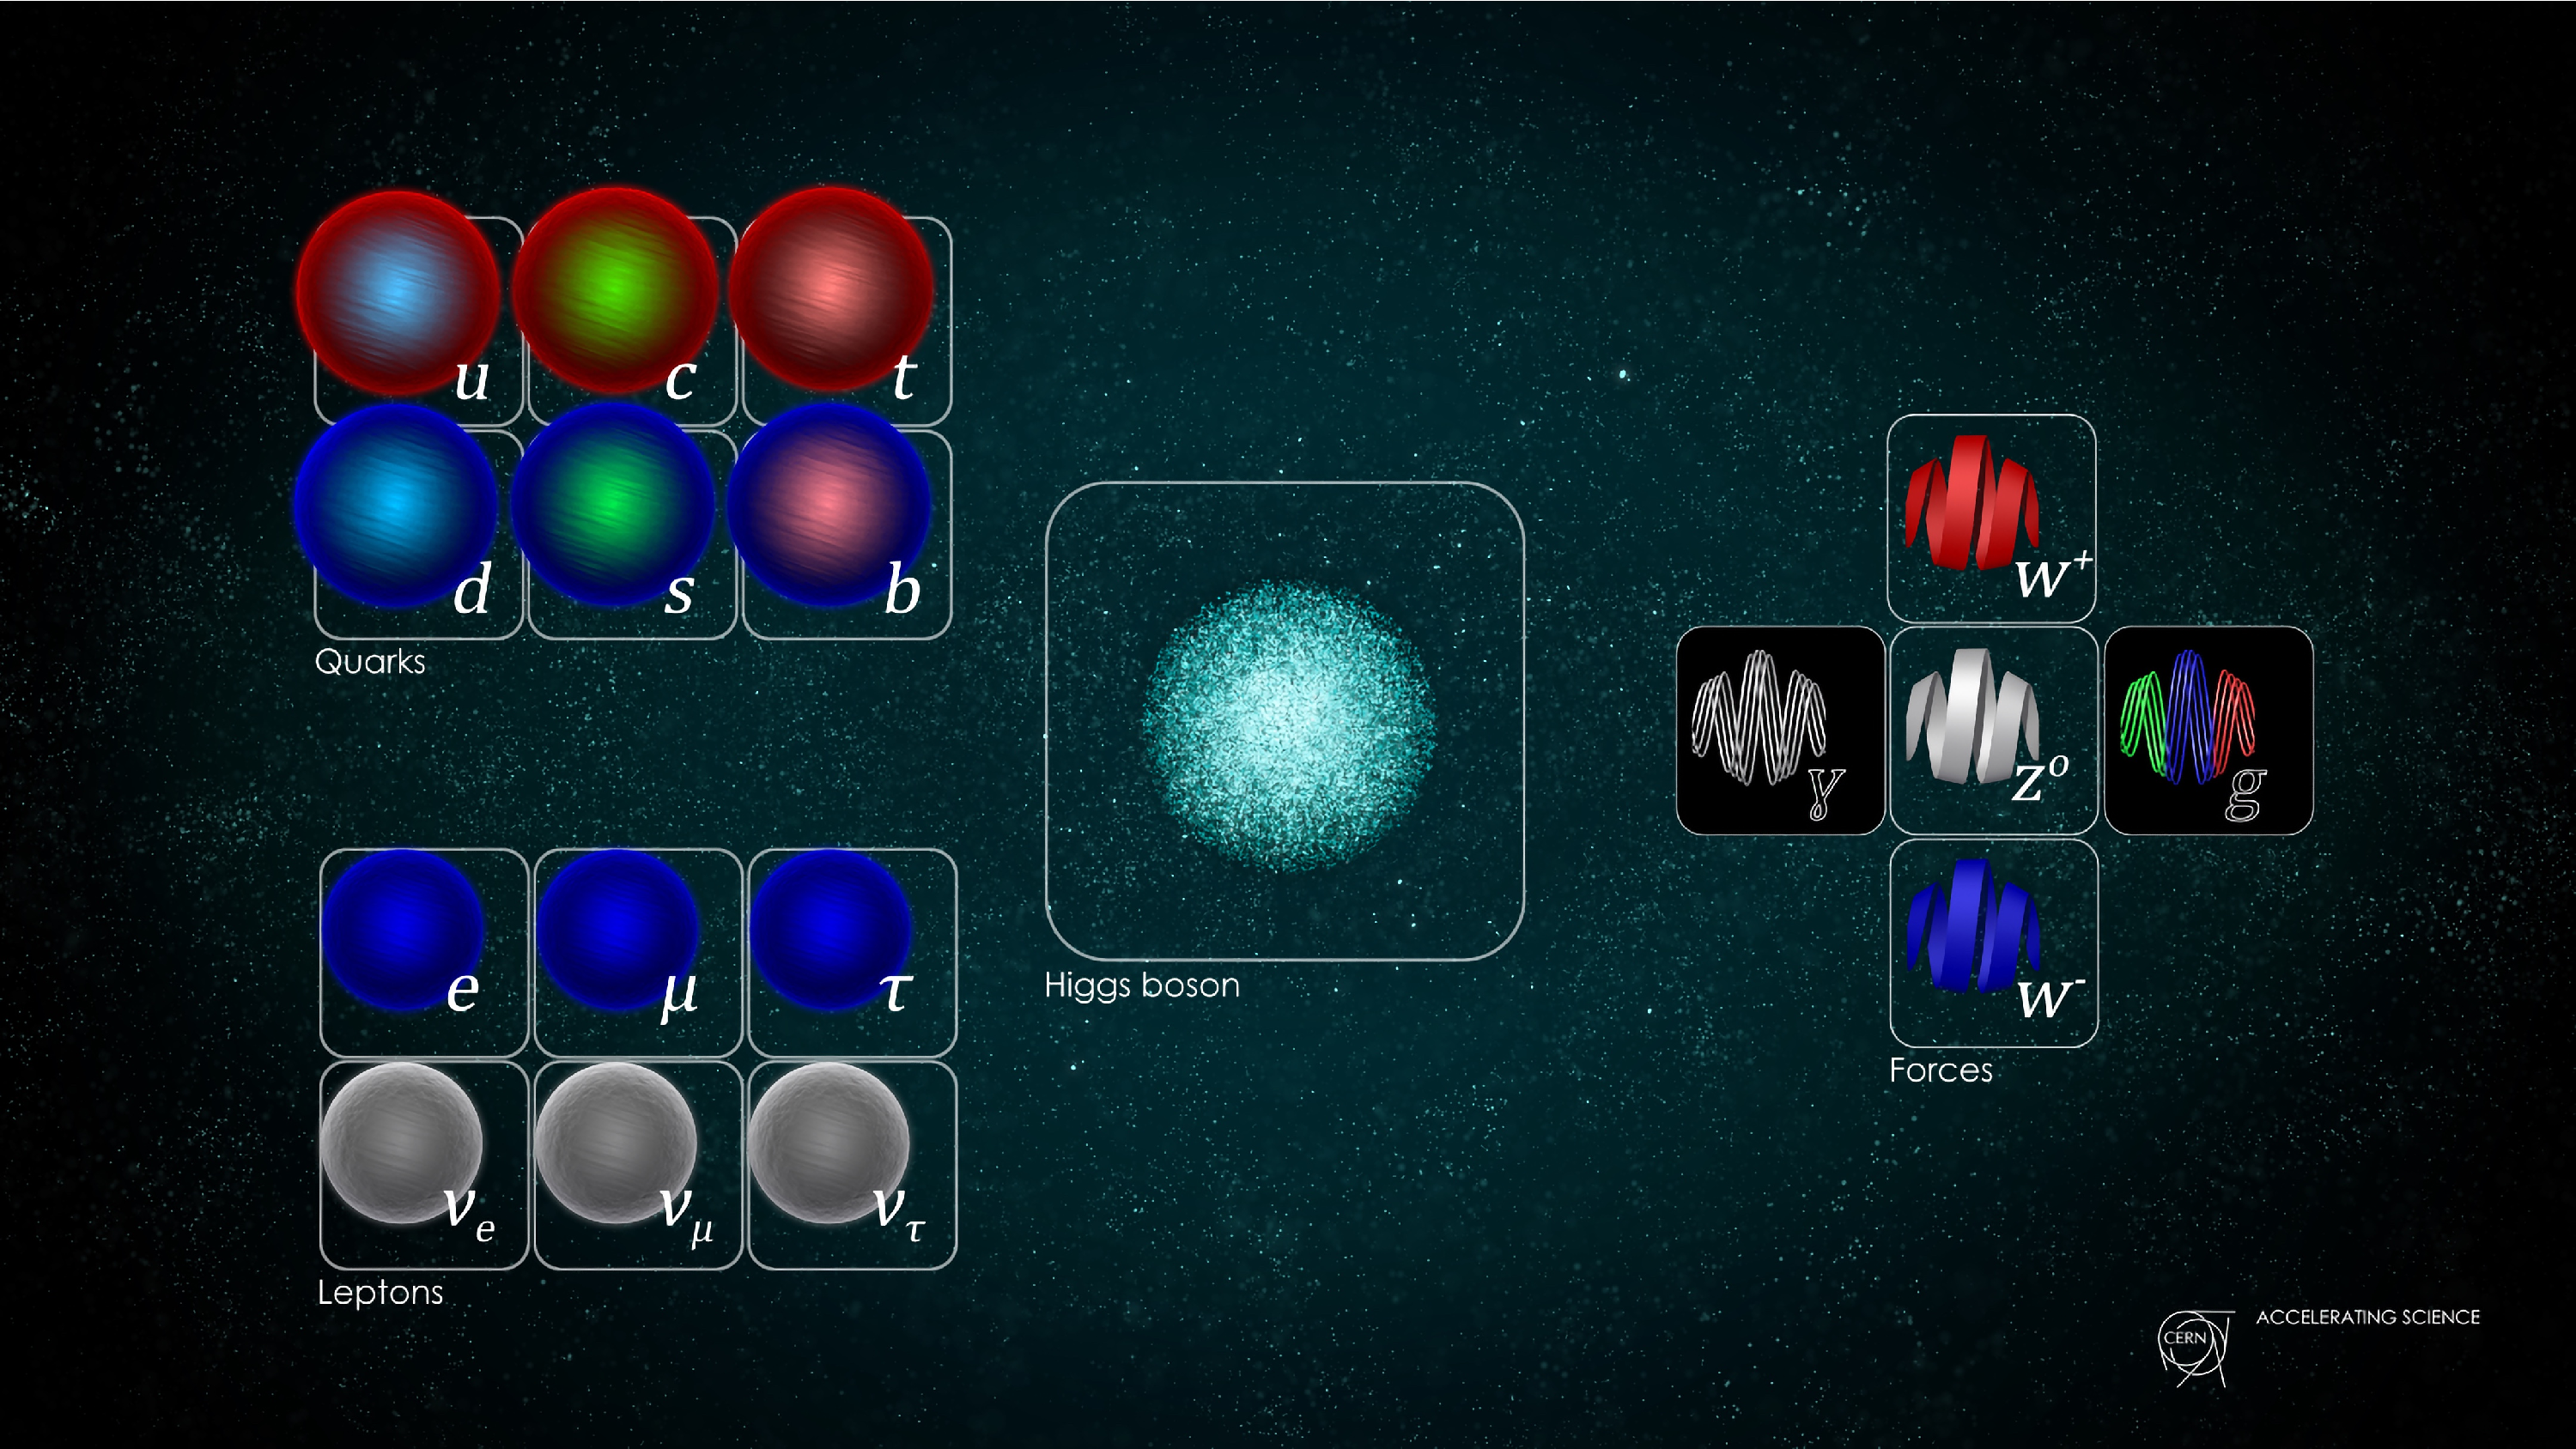
\includegraphics[width=0.9\linewidth]{files/StandardModel.pdf}
 	\caption{The Standard Model of Particle Physics\ \cite{cern_SM}.}\label{StandardModel}
\end{figure}

A first limitation of the Standard Model lies in its inability to provide a quantum description of gravity. A force-carrier of the gravitational force, the graviton, was hypothesized but not yet observed. The most accurate description of gravity remains the General Relativity, yet no framework currently exists that successfully unifies it with the Quantum Field Theory description of the Standard Model.
A second limitation arises from the fraction of the Universe that the Standard Model can account for. Indeed, only 5 $\%$ of the Universe, known as the baryionic matter, can be described, there is roughly 27 $\%$ of the Universe which is composed of so-called Dark Matter that the Standard Model is today unable to explain nor describe. The remaining 68 $\%$ of our Universe is made up by Dark Energy and is associated to the vacuum in space, yet its nature remains widely unknown too.\\

Aware of these limitations, physicist were first looking for outstanding phenomena that have been mostly ruled out by now. Significant efforts are being made towards precision measurement of the current theory in order to either further confirm the predictions or find inconsistencies hinting at unexplained phenomena and thus new Physics. For this reason, an upgrade of the current accelerator, the Large Hadron Collider (LHC), the High-Luminosity-LHC (HL-LHC) was proposed in order to obtain a fivefold increase of the instantaneous collision rate and a tenfold increase of the integrated luminosity with respect to the nominal LHC design values\ \cite{HL_LHC_report}.\\

Another limitation of the current LHC experiments like ATLAS or CMS is the geometrical acceptance their design can achieve. Indeed, the detectors are arranged in a cylindrical pattern centered around the LHC beam pipe, the detectors are hence very effective to detect heavy particles produced with large transverse momentum. On the contrary, if light particles were to be created in the very forward direction, they could be contained within the uncovered portion of space occupied by the beam pipe itself. Until proof of the contrary, some new Physics could also be hiding in these un-instrumented regions and some experiments already intend to use this incomplete acceptance to probe signals from weakly interacting and Long Lived Particles (LLPs) as suitable candidates for Dark Matter (DM).    
\clearpage 

\section{The FASER Detector: Looking Forward for New Physics}
The ForwArd Search ExpeRiment (FASER) is a detector located \SI{480}{\meter} downstream of the ATLAS Interaction Point (IP), benefiting from the curvature of the LHC to probe LLPs emitted in the very forward direction, initially contained within the uncovered acceptance of the experiment. 
The FASER detector was originally designed to detect charged decay of LLPs such as Dark Photons into an electron-positron pair. Although, in its current state, the detector is not able to distinguish between events in which one or more photons are produced. The FASER collaboration hence proposed in 2021 an upgrade of the original Preshower sub-detector with a high precision Tungsten-Silicon (W-Si) Preshower displaying its ability to resolve di-photons events from the decay of Axion-Like Particles (ALPs)\ \cite{PreShower_TP}. \\

The work presented in this thesis will first guide the reader through a description of the FASER detector and its original layout for the detection of charged decay products from LLPs. The reader will then be presented with the Physics program of FASER and why it was essential to unlock its potential for detection of neutral decay products such as di-photon signals. A theoretical description of an ALP model used for the proposal of the Preshower upgrade will then be given. The discussion will start with the motivation for ALPs, move to a phenomenological description of the specific ALP model simulated for this purpose and will finish with ALP production and decay within the FASER detector. 

\section{Development of Monolithic Silicon Pixel Detectors for HEP.}
\subsection{Motivation for a new detector technology}
The recent achievement in semiconductor technologies, and especially silicon-based devices, have paved the way for the development of the new detector technologies needed to overcome the challenges of future experiments. The important increase in number of collisions will be a real challenge for the experiment built within the specifications of the nominal LHC parameters. A complication that will need to be addressed is the increase in pile-up, the phenomenon in which the detector is not able to distinguish between tracks coming from different collisions of protons within the bunches. So far, particle tracking systems were relying only on the 3D information to deal with pile-up events, but the amount of such events will increase from roughly 50 up to 200 with the HL-LHC characteristics\ \cite{PhaseII_Atlas}.

The discriminating criteria to associate tracks to the correct collisions lies in the timing information associated to the reconstructed particle tracks, making these particle tracking systems 4D-trackers. The pile-up events are mostly contained within a time window of not more than \SI{200}{\pico\second}, slicing the beam crossing spot in consecutive exposures of \SI{30}{\pico\second}, the number of vertices per exposure would drop to current LHC pile-up levels\ \cite{PhaseII_CMS}. Some experiments like ATLAS\ \cite{PhaseII_Atlas} or CMS\ \cite{PhaseII_CMS} already foresee an upgrade of the detector layout including a timing layer in the pseudo-rapidity regions where the pile-up is the most important. \\

Traditionally, in order to obtain a time resolution of the order of tens of picoseconds, gas detectors such as the Multigap Resistive Plate Chambers (MRPCs) designed for the Alice Time Of Flight (TOF) detector\ \cite{MRPCs_AliceTOF}, have been a suitable solution. Although, the design and performance of such detectors is not compatible with the requirements of the 4D trackers. Indeed, as the trackers are located very close to the beam interaction point, they need good spatial resolution combined with a compact design but among all a capability to sustain high detection rates. Silicon based detectors offer many advantages in this regard which will later be discussed in \chref{ch:2}. \\

At the University of Geneva (UniGe), the development of monolithic silicon pixel detectors for timing applications has started in 2016 under the TT-PET project which proved that monolithic sensors can be used to reach time resolution of the order of \SI{110}{\pico\second} \cite{TTPET-110ps}. This already impressive performance was further improved over the years, now under the MONOLITH project, reaching in 2023 a time resolution of \SI{20}{\pico\second} for a sensor without internal gain layer. The sensor also demonstrated to remain fully efficient and offer time resolutions of the order of \SI{50}{\pico\second} even when operated at very low power densities of \SI{150}{\milli\watt/\centi\meter^2} \cite{Monolith_20ps}.

The breakthrough in performances can be associated to the implementation of Silicon Germanium Hetero Bipolar Transistors (SiGe HBTs) to produce very fast and low noise frontend electronics. The combination with monolithic implementation offers a sustainable solution, benefiting from the simplified assembly process and reduced production cost of monolithic designs in commercial Complementary Metal Oxide Semiconductor (CMOS) processes used in large-volume silicon foundries.

\subsection{Monolithic sensors for ultra-fast timing}
The MONOLITH project at UniGe aims at developing a new generation of monolithic silicon pixel detectors, improving the intrinsic time resolution limit of roughly \SI{30}{\pico\second} of current designs by an order of magnitude and providing at the same time high spatial resolution. 

The work presented in this thesis will first guide the reader through a description of semiconductors and how these can be used for particle detection. The formation of signal and its reading out will be presented alongside a comparison of hybrid and monolithic pixel detectors. This introductory part will be concluded by a discussion of the relevant factors to characterize radiation tolerance of this technology. 

Subsequently, the work performed for the characterization during testbeam campaigns at the SPS facility at CERN of two prototypes will be presented. The layout of the test set-up as well as the data taking methods will be introduced to further discuss the measurement of detection efficiency and timing resolution of these prototypes, notably under low power density operation.   

Finally, the radiation tolerance of the second prototypes discussed above will be discussed, again through some test at the SPS facility at CERN. The effect of different doses and the change in detection efficiency and timing resolution will be presented and discussed. 


\subsection{Monolithic sensors for TeV-scale photon detection }
The upgrade of the FASER Preshower detector can profit from the developments already achieved in monolithic silicon pixel detector technology to develop a high granularity silicon preshower detector. This design choice will reduce the overall cost and complexity of the upgrade that hybrid sensors would typically introduce. A dedicated front-end, still benefiting from the low noise performances of SiGe HBTs can be implemented to offer a sufficiently large dynamic range needed to resolve di-photons events in the detector. 

This part of the thesis will focus on the description of the FASER Preshower detector. The discussion will start by a description the requirements of the ASIC and how these influenced its design. The structure of the detector will be presented, along with the subdector components, the planes, and their subdivisions into modules, themselves composed of ASICs. The detector control and readout will also be presented to complete the description of the detector. 

The reader will then be presented with the diverse test performed in order to develop and assemble the FASER preshower detector. The discussion will start with the description and characterization of a pre-production ASIC, designed specifically to refine and test different design choices, leading to a description of the production ASIC. The qualification and commissioning of the detector will present the different assembly stages together with the characterization of ASICs and modules prior to installation. The development of the trigger and data acquisition software will be presented together with first results from testbeam campaigns demonstrating the functioning of the ASIC, its powering and its data acquisition system. 

\clearpage

\chapter{FASER: Looking forward for Long-Lived-Particles}
	The Standard Model has proven to be one of the most successful theories in Physics but still fails to address several key phenomena, including the nature itself of DM. This fondamental shortcoming have motivated physicists to explore theoretical extensions of the SM predicting new particles and providing potential DM candidates, many of which remain hidden from current collider experiments due to the their predicted masses but also their often weak coupling to the SM. 

	In the past decades, searches for Beyond the Standard Model (BSM) physics at the LHC was focused on heavy particles in the TeV-scale mass range and couplings to the SM of the order of $\mathcal{O}(1)$. These particles were expected to be produced with large transverse momentum ($p_T$), making large cylindrically symmetric general purpose experiments like ATLAS \cite{atlas_detector} and CMS \cite{cms_detector} the best candidates for detection BSM candidates. 
	
	After many years of searches in this direction, the absence of discoveries opened the floor to an increasingly compelling class of BSM models predicting new particles both light and weakly coupled to the SM \cite{FASER_LLP}, providing good DM candidates. An important aspect of such models is found in the predicted $p_T$ of the particles with masses in the range of MeV-scale to GeV-scale, which can be of the order of $p_T ~ 100$ MeV - GeV and is considerably smaller than the $p_T$ for models predicting particles whose mass belong to the TeV-scale. These particles would hence be produced in what is called the very forward region, making actual searches with experiments like ATLAS completely misguided due to its pseudorapidity coverage roughly limited to $|\eta| \lesssim 2.5$.
	
	This new class of BSM particles often arise in well-motivated models such as hidden sectors connected to the SM via portals—e.g., dark photons (vector portal), axion-like particles (ALPs, pseudoscalar portal) which will be discussed more in details in \note{insert section}, or dark Higgs bosons (scalar portal). At first glance, the extremely weak couplings of these particles to the SM may seem like a showstopper, unless the rate of events from which these particles are originating was sufficiently high. Taking as a benchmark the LHC at $\sqrt{s} =$ \SI{13}{\tera\electronvolt}, the total inelastic proton-proton cross section is approximately $\sigma_{inel}($\SI{13}{\tera\electronvolt}$) \approx 75 \text{ mb}$ \cite{inelastic_XS_ATLAS} of which most it is in the forward direction. The cross section is very similar for the LHC at $\sqrt{s} =$ \SI{14}{\tera\electronvolt} and for an integrated luminosity of 150 fb$^{-1}$, the expected number of inelastic proton-proton scattering is expected to be
	\begin{equation}
		N_{inelastic} \approx 1.1 \cdot 10^{16}
	\end{equation} 

	resulting in extraordinary meson production rates as for example $N_{\pi^0} \approx 2.3 \cdot 10^{17}$ and $N_{B} \approx 7.1 \cdot 10^{13}$ \cite{FASER_LLP}. This means that even with small branching ratios and extremely weak coupling to the SM, these models might still provide a sufficient number of events in the very forward region and make this new search channel promising.  Another crucial property of these particles is their long lifetime as a resulting consequence of their weak SM coupling. Before possibly decaying into SM particles, these LLPs would then be able to travel long distances, a necessary condition for them to be able to exit the LHC beam pipe and decay into a long-baseline forward region detector. Furthermore, the characteristic production angle for particles originating from $\pi^0$ and B mesons is approximately:  
	\begin{equation}
    	\theta \sim \frac{m}{E} \quad \text{or} \quad \frac{\Lambda_{\text{QCD}}}{E},
	\end{equation}
	where $\Lambda_{\text{QCD}} \sim 200~\mathrm{MeV}$ and $E$ is typically in the TeV range, resulting in $\theta \sim 100~\mu\mathrm{rad}$. This implies that forward LLPs remain tightly collimated along the beam collision axis, and their transverse spread remains limited to within $\sim$ 10-\SI{50}{\centi\meter} even after traveling several hundred meters downstream. 
	
	These observations form the foundation for the design of the ForwArd Search ExpeRiment (FASER). Strategically located \SI{480}{\meter} downstream from the ATLAS IP in the TI12 tunnel—originally used for beam injection from the SPS, FASER is co-axial with the LHC collision axis and exploits the LHC’s natural beam curvature to isolate the path of LLPs. This location allows it to be shielded from most of the SM backgrounds, while being ideally positioned to intercept the otherwise undetectable forward flux of new particles.
	
	\begin{figure}[H]
    	\centering
    	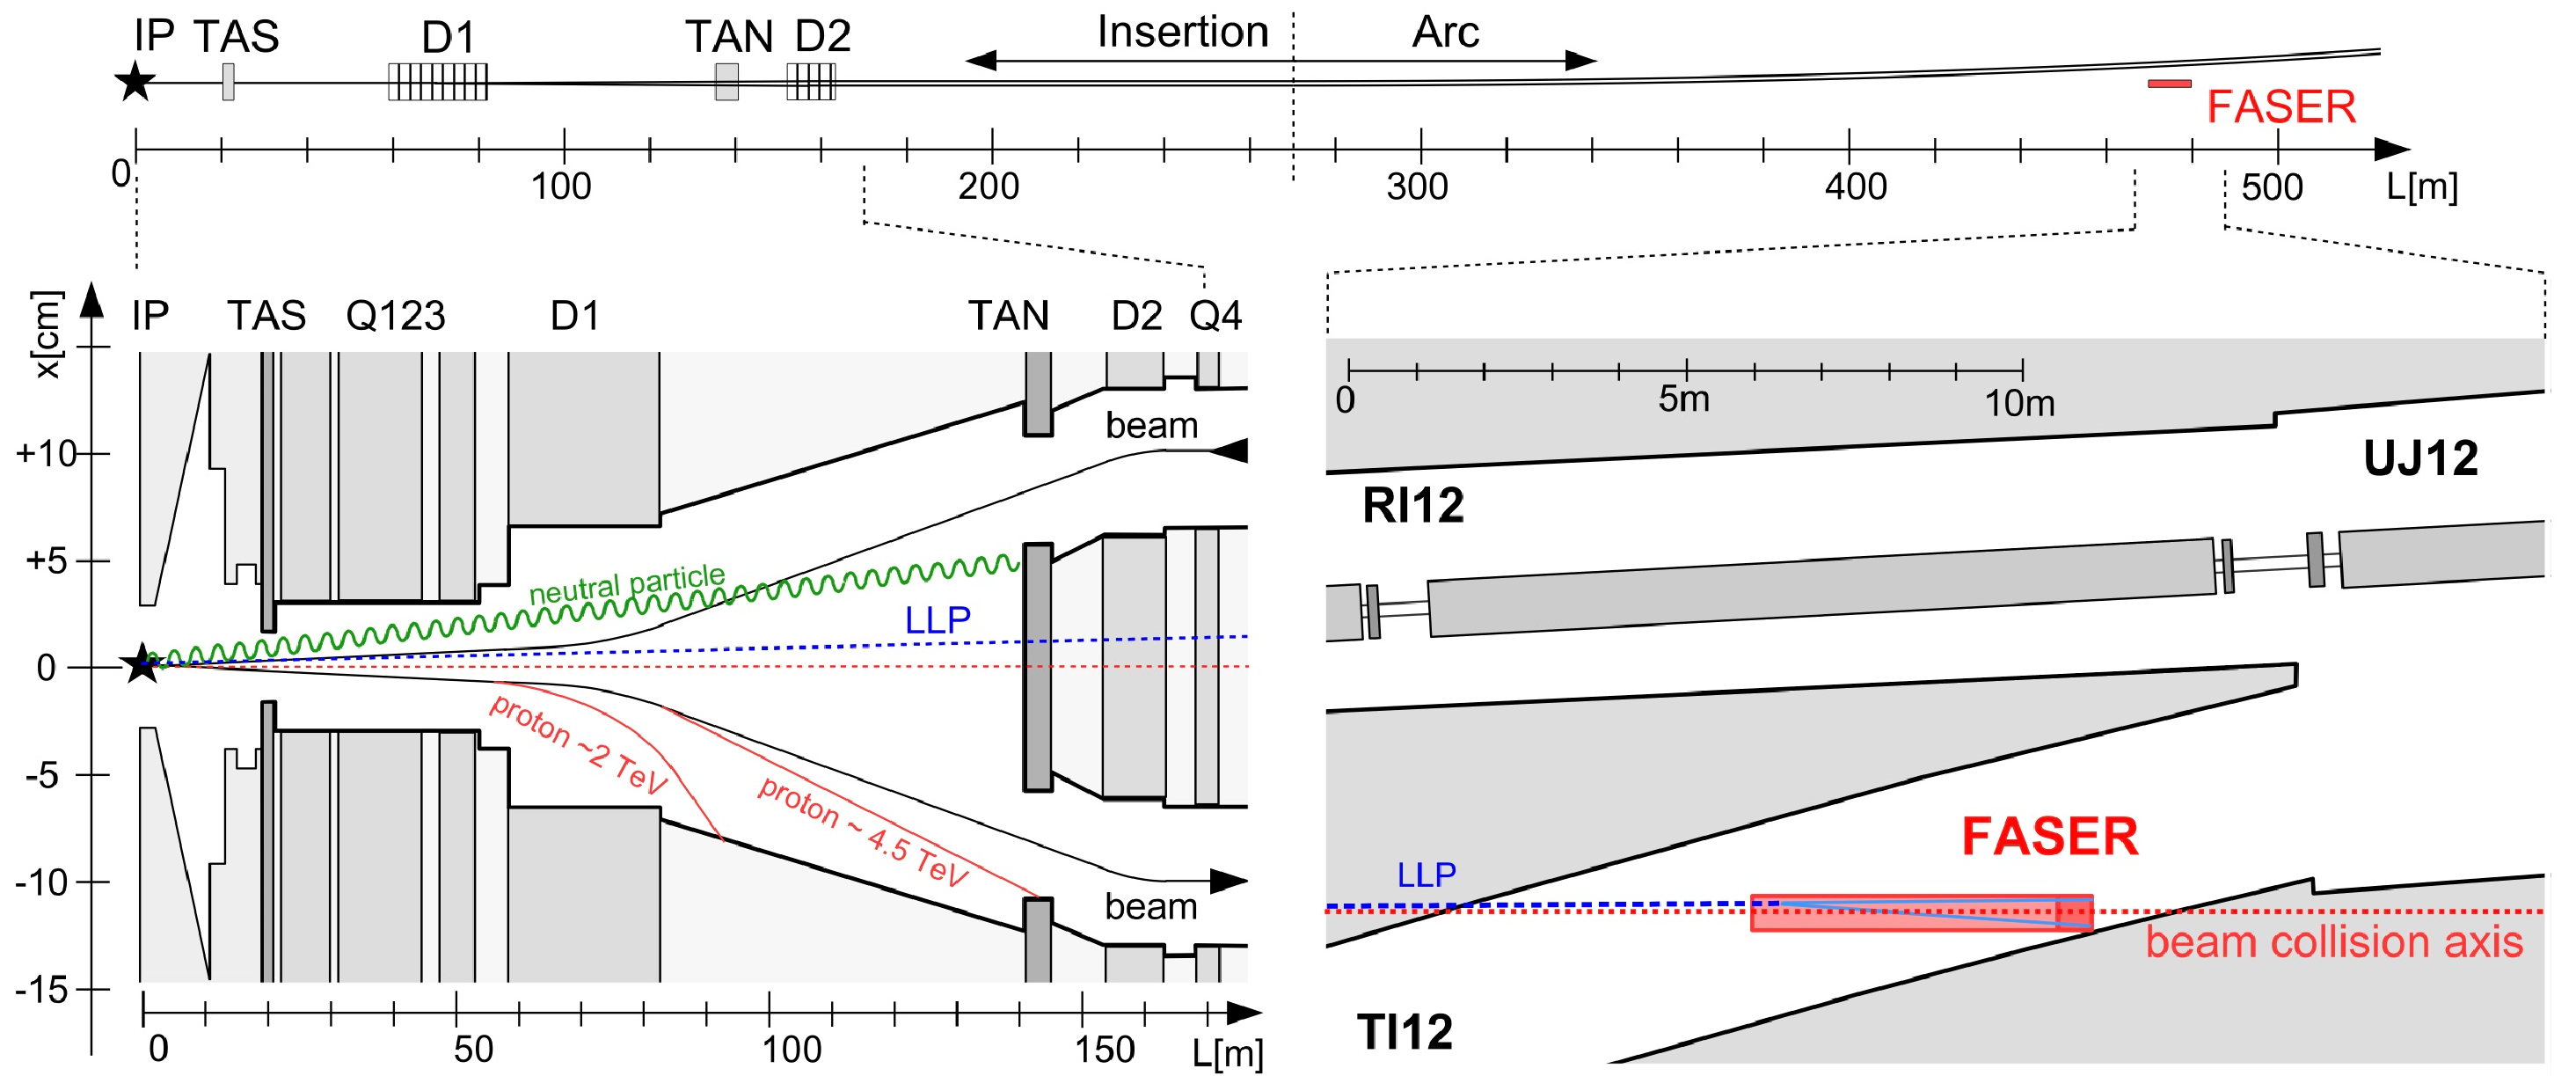
\includegraphics[width=0.9\textwidth]{files/FASER_location}
    	\caption{Location of the FASER detector in the TI12 tunnel, \SI{480}{\meter} downstream of the ATLAS IP. The beam bending in the arc creates a clear line of sight for particles produced in the far-forward region.}
    	\label{fig:faser_location}
	\end{figure}
	
	In this context, FASER serves as a complementary approach to more conventional LHC experiments. It enables probing of new regions of parameter space, particularly for low-mass, long-lived, and weakly coupled particles. Its small footprint and cost-effective design make it an attractive model for future LLP searches, and its results are expected to provide crucial insights into the hidden sector. In the following chapter at first will come a presentation of the physics potential of FASER as a probe of the hidden sector for discovery of potential DM candidates. An overview of the FASER detector along with its background from the SM and typical signatures for LLP decays. Finally, the emphasis will be put on an ALP model in which the particle is produced through rare meson decays and decays into two photon within FASER, building ground for the proposal on an upgrade of a sub-component of the original detector layout: the PreShower. 
	
	\clearpage
	
	\section{Physics program: A probe to the Hidden sector and more}
	The location of the FASER detector provides reach to a wide range of LLP models decaying into SM particles with energies in the TeV range. It also provides a novel measurement of neutrino interactions when produced at colliders. In the following section, a presentation of the different production mechanisms for LLPs as well as two leading LLP model probed by FASER will be presented, a complete overview of FASER's reach for LLPs is presented in \cite{FASER_LLP} with various benchmark models used to motivate the need for an experiment such as FASER. The motivation is further complemented through the study of neutrinos reaching FASER and equivalently, a detailed study can be found in \cite{neutrino_FASER}.  
	
		\subsection{Production of LLPs}
		Multiple production mechanisms are responsible for the production of new light particles at the LHC, including rare decays from light and heavy hadrons, dark bremsstrahlung in coherent proton-proton collisions, direct production in hard scattering: FASER being located after a neutral particle absorber (TAN), the particles created at the ATLAS Interaction Point (IP) may travel \SI{140}{\meter}, interact with the TAN and make it a beam dump experiment \cite{FASER_LLP}. The Feynman diagrams for each production mechanism are presented below and will be used along the upcoming discussion \cite{FASER_LLP}.
		\begin{figure}[h]
			\centering
			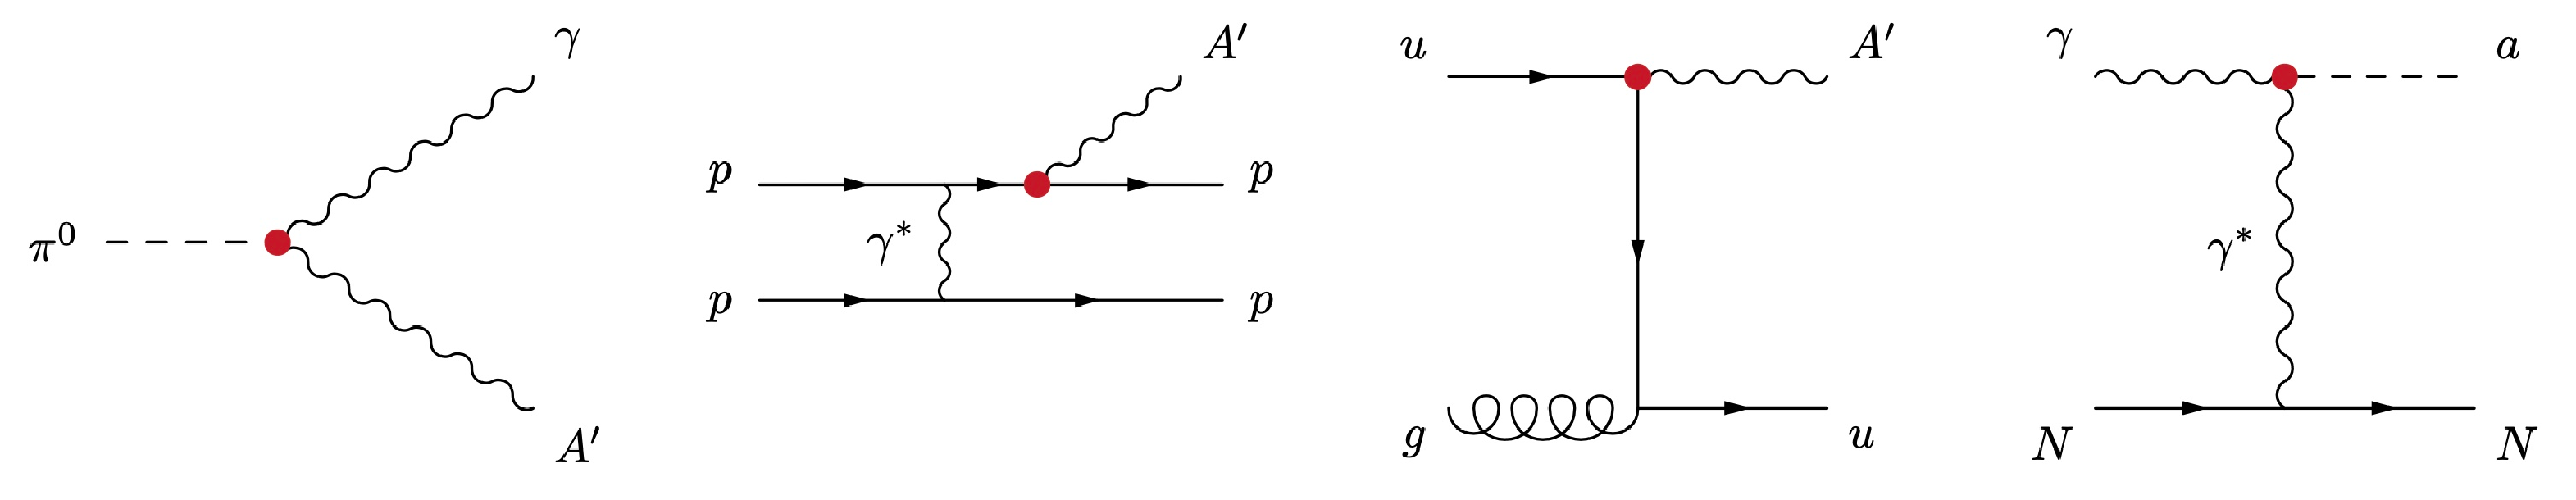
\includegraphics[width=0.95\linewidth]{files/Feynman_production_mechanism}
			\caption{From left to right, production mechanisms via: rare meson decay, dark bremsstrahlung, hard scattering and Primakoff process from photon in the TAN.}
			\label{im:prod_mech_feynman}
		\end{figure}
		\subsubsection{Rare meson decays}
		The large hadron flux from the ATLAS IP in the very forward direction makes the production of LLP coupled to quark a prominent production mechanism through rare decays into LLPs from hadrons kinematically compatible. 
	
		The flux of light hadron is mainly composed of neutral pions ($\pi^0$) and eta mesons $\eta$ with respectives cross sections of $\sigma_{\pi^0} = 1.6 \times 10^{12}$ pb and $\sigma_{\eta} = 1.7 \times 10^{11}$ pb. Alternatively, the flux of heavy hadrons mainly composed of D-mesons and B-mesons with respectives cross sections of $\sigma_{B} = 7.4 \times 10^{9}$ pb and $\sigma_{D} = 4.7 \times 10^{8}$ pb. As shown before, these particles are emitted in the very forward direction with a very small angle with respect to the beam axis. The spectrums for the production of $\pi^0$ and B-mesons in the $(\theta, p)$ plane with $\theta$ the emission angle of the meson with respect to the beam axis and $p$ their momentum is presented in the figure \ref{im:hadron_flux}  \cite{FASER_LLP}.
	 	\begin{figure}[h]
			\centering
			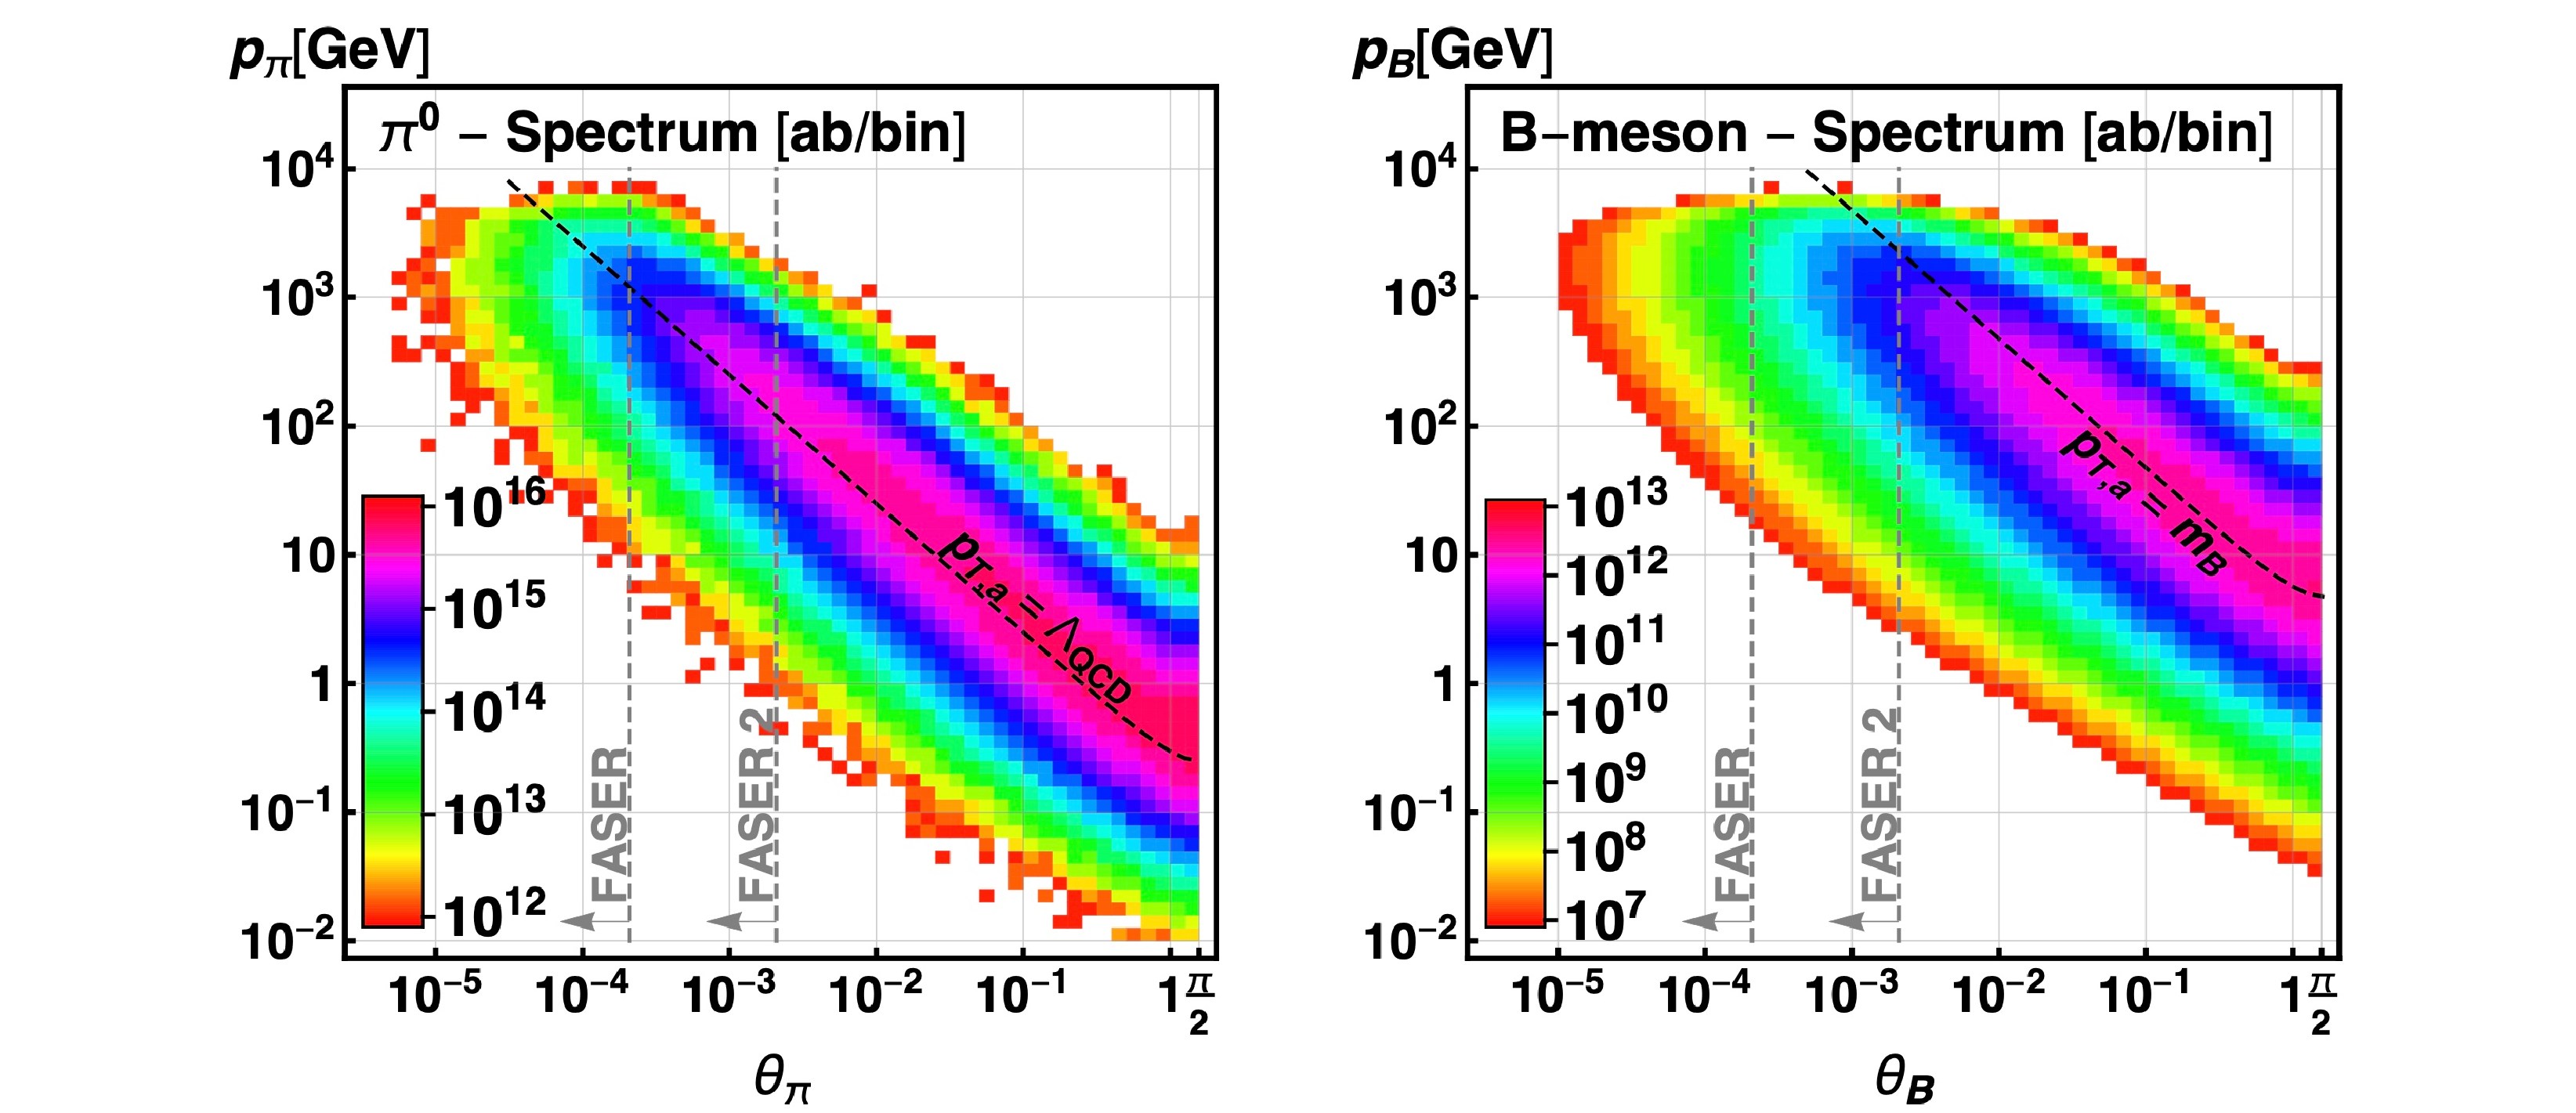
\includegraphics[width=0.95\linewidth]{files/pi0_B_meson_flux}
			\caption{Differential meson production rates in the $(\theta, p)$ plane with $\theta$ the emission angle with respect to the beam axis and $p$ their momentum. The angular acceptance of FASER and a potential upgrade, FASER2 are shown as dashed vertical grey lines.}
			\label{im:hadron_flux}
		\end{figure}

		
		\subsubsection{Dark Bremsstrahlung}
		If LLPs were to be heavier than the kinematic threshold for production via decay, their production could be dominated by what is called dark bremsstrahlung in proton-proton scattering as show in \ref{im:prod_mech_feynman}. This production is particularly relevant for dark vector bosons $V$ for masses of the LLP such that $m_V > m_\pi$. For other types of models, a different production mechanism put shade onto the dark bremsstrahlung put it sill contributes with a subdominant role. 
		
		\subsubsection{Hard scatterings}
		At the parton level, a plethora of hard scatterings between the constituents of the protons can produce LLPs as illustrated in \ref{im:prod_mech_feynman}. The large incertitudes on the parton distributions functions at low momentum transfer makes an accurate LLP production rate estimation difficult through this channel \cite{FASER_LLP}. On the contrary, if the mass of the LLP would be such that $M_{LLP} >$ \SI{2}{\giga\electronvolt}, the Drell-Yann process could become dominant as discussed in \cite{Drell_Yann}. In what follows, this production mechanism will not be considered. 
		
		\subsubsection{"Beam Dump" production}
		
		The large number of particles produced in the very forward region that can travel \SI{140}{\meter} before interacting with the TAN produces a fixed-target beam dump experiment able to produce LLPs. One particularly dominant process is the Primakoff process for which photons copiously produced at the ATLAS IP interact with the TAN and produce an LLP as show in \ref{im:prod_mech_feynman}. Figure \ref{im:photon_ATLAS_ALP} (left panel) shows the spectrum for production of photon from the ATLAS IP. The acceptance of the TAN set a constraint at the level of $\theta_a < 10^{-3}$ for photons to interact \cite{Primakoff_process}. Similarly, dark vector bosons $V$ could be produced via dark Compton scattering ($ \gamma e^- \rightarrow V e^-$) but this process remains subdominant with respect to other production mechanisms. 
	
		
		\subsubsection{LLPs reaching FASER}
		Once produced, an LLP of mass $m$  with an angle $\theta$ and momentum $p$ with respect to the beam axis, has a probability of decaying within FASER given by geometrical acceptance such that: 
		\begin{equation}
			\mathcal{P}(\theta, p) = {\left( e^{-(L-\Delta)/d} - e^{-L/d}\right)} \hspace{1mm} \Theta \left(R-L\tan(\theta)\right) \approx \frac{\Delta}{d}e^{-L/d} \hspace{1mm} \Theta \left(R-L\tan(\theta)\right)
		\end{equation}
		where $L$ denotes the distance between IP and FASER, $R$ the radius of the detector and $\Delta$ the length of the decay volume. The variable $d$ is defined as the decay length of the LLP in the lab frame and can be written as $d = c \tau \beta \gamma$ with $\tau$ the LLP's lifetime. The number of LLPs decaying inside FASER can then be written as \cite{FASER_LLP}: 
		\begin{equation}
			N_{\text{LLP decay}} = \mathcal{L} \int dp \hspace{1mm} d\theta \frac{d\sigma_{pp \rightarrow LLP + X}}{dp \hspace{1mm} d\theta} \cdot \mathcal{P}(\theta, p)
		\end{equation}
		
		In the following discussion for different benchmark models in the physics reach of FASER, the decay of LLP into invisible dark sector particles will be neglected so that only detectable event rate can be quoted. Additional contributions such as detection efficiency will be neglected and set at 100 \% for the ease of comparison with other experiments. 
		
		
		\subsection{Vector Portal: Dark photon}
		On of the best motivated LLP model includes the addition of a U(1) symmetry with renormalizable coupling and the corresponding vector field $X_\mu$ coupling through kinetic mixing to the SM hypercharge gauge bosons  or at low energies to the SM photon \cite{FASER_LLP}. The dark photon model emerges from this completion of the SM and the Lagrangian is extended as: 
		\begin{equation}
			\mathcal{L} = \mathcal{L}_{SM} + \frac{1}{2} m'^2X^2 - \frac{\epsilon'}{2}F_{\mu \nu}F'^{\mu \nu}
		\end{equation} 
		
		where $\epsilon'$ parametrises the kinetic mixing term and $F_{\mu \nu}$ and $F'^{\mu \nu}$ are the field strength tensor of the SM photon and $X$ the one of the new gauge boson. After rotation into the mass basis, the photon-SM fermion coupling parameter is given by $\epsilon = \epsilon' \cos{\theta_W}$. Removing the kinetic mixing term after a field re-definition, the dark photon field $A'$ emerges as a physical mass eigenstate coupling to charged SM fermions through their electric charge so that \cite{FASER_LLP}: 
		
		\begin{equation}
			\mathcal{L} = \mathcal{L}_{SM} + \frac{1}{2} m_{A'}^2A'^2 - \epsilon e \sum_f q_f \bar{f} \gamma_\mu A'^\mu f 
		\end{equation} 
		
		where $g_f$ is the charge of the fermions and $f$ (and $\hat{f}$) the field of the fermions themselves. As discussed before, the dark photon may be produced both through rare decays of light mesons (at low values of $m_{A'}$) like $\pi , \eta \rightarrow \gamma A'$ and also at higher masses predominantly by dark bremsstrahlung. These processes are neglected with respect to the SM counterparts roughly by a factor $\epsilon^2$ \cite{FASER_LLP}. \\ 
		
		Once produced, the dark photon may decay into a pair of charged leptons, for the smallest masses to a $e^+ \hspace{1mm} e^-$ pair if $m_{A'} > 2m_e$ and other heavier pairs, even hadronic if the kinematic conditions are met.The partial decay width for the dark photon into an $e^+ \hspace{1mm} e^-$ pair is given by \cite{dark_photon_Feng} : 
		\begin{equation}
			\Gamma (A' \rightarrow e^+ \hspace{1mm} e^-) = \frac{\epsilon^2 e^2 m_{A'}}{12 \pi} \left[ 1-\left( \frac{2m_e}{m_{A'}} \right)^2 \right]^{1/2} \left[ 1 + \frac{2m_e^2}{ma_{A'}^2} \right] 
		\end{equation}
		The total dark photon decay width can then be obtained through the use of the branching ratio of dark photon into $e^+ \hspace{1mm} e^-$ pair $\mathcal{B}(A' \rightarrow e^+ \hspace{1mm} e^-)$ so that it reads: 
		\begin{equation}
			\Gamma_{A'} = \frac{\Gamma (A' \rightarrow e^+ \hspace{1mm} e^-)}{\mathcal{B}(A' \rightarrow e^+ \hspace{1mm} e^-)}
		\end{equation}
		In the limit in which $E_{A'} \gg m_{A'} \gg m_e$ the dark photon decay length can then be written as: 
		\begin{equation}
			\bar{d}_{A'} = c \frac{1}{\Gamma_{A'}} \gamma_{A'} \beta_{A'} 
%			\approx \text{(80 m)} \mathcal{B}(A' \rightarrow e^+ \hspace{1mm} e^-) {\left[ \frac{10^{-5}}{\epsilon} \right]}^2 {\left[ \frac{E_{A'}}{\text{TeV}} \right]} {\left[ \frac{100 \text{ MeV}}{m_{A'}} \right]}^2
		\end{equation}
		
		The dark photon decay length, branching fractions into leptonic and (heavier) hadronic states are shown in the left panel of figure \ref{im:dark_photon_prod}. The sensitivity reach in the $m_{A'}$ and $\epsilon$ parameter space for FASER for dark photons is presented in the right panel of figure \ref{im:dark_photon_prod} together with a comparison between the already excluded regions (in grey), current and future experiments.
		\clearpage
		\begin{figure}[h]
			\centering
			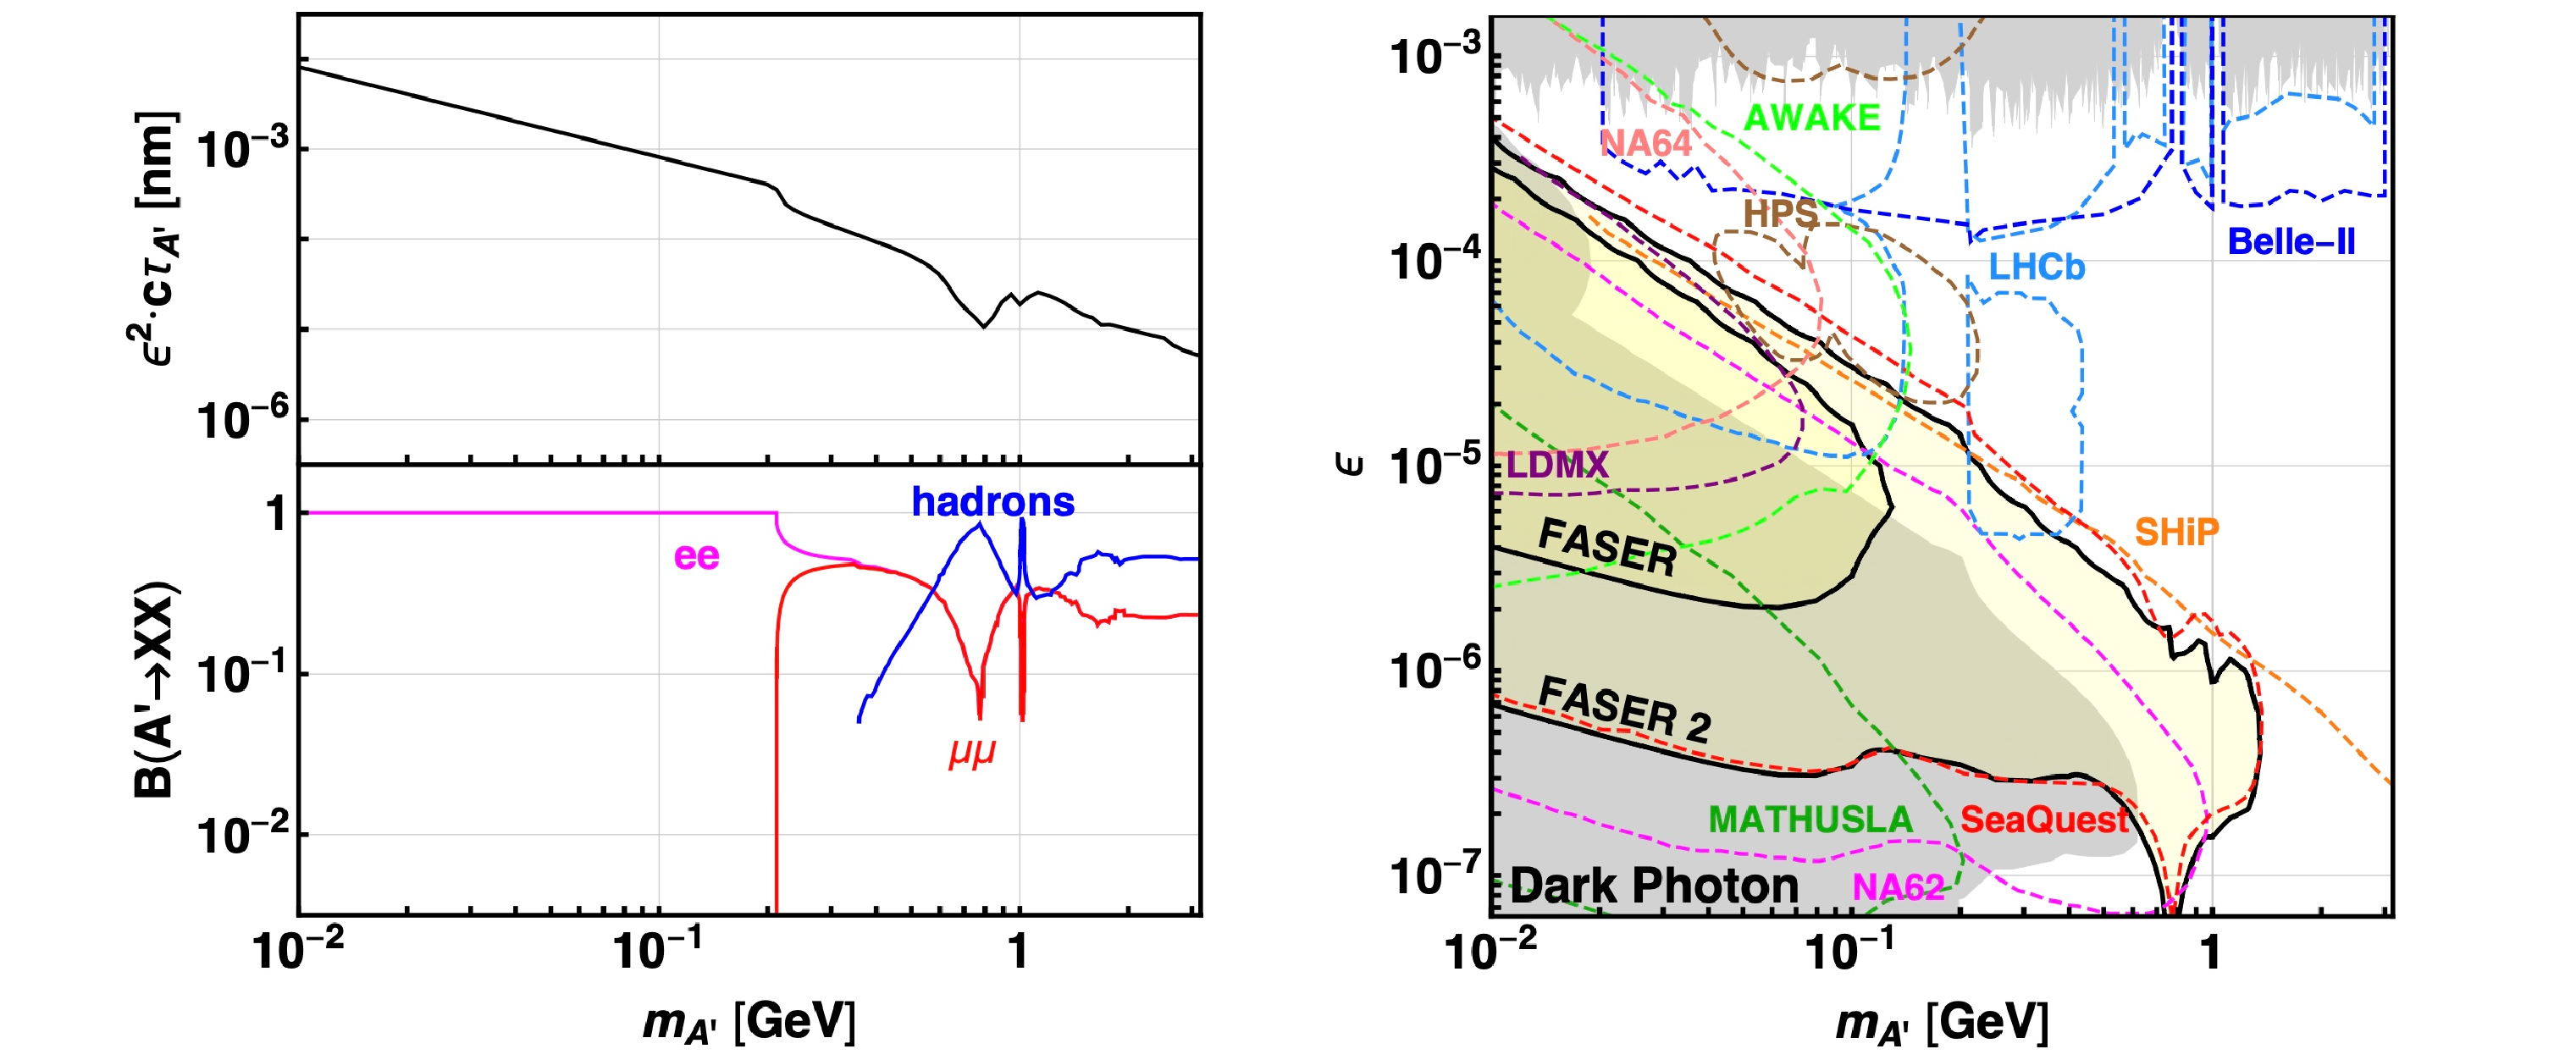
\includegraphics[width=0.95\linewidth]{files/dark_photon_production}
			\caption{The dark photon decay length (top left panel), its branching fractions in diverse possible final states (bottom left panel) and FASER's reach in the dark photon parameter space defines by its mass and kinetic mixing parameter}
			\label{im:dark_photon_prod}
		\end{figure}
		
		A detailed interpretation of the sensitivity reach presented is given in \cite{FASER_LLP} but is is striking to see that FASER will already be able to probe an interesting section of the parameter space throughout the LHC Run 3. The boundary at very low mixing parameter is given by the $\epsilon^4$ dependence of both production and decay mechanisms, both happening through the mixing of the dark photon to SM fermions. On the other hand, the boundary for high mixing parameter becomes exponentially suppressed as the dark photon will decay before even reaching the detector \cite{FASER_LLP}.  
		
		
		\subsection{Pseudoscalar Portal: Axion Like Particles}
		
		Axion-Like-Particles differ from other models through the dimension-5 operators through which they couple to the SM. They manifest themselves as pseudo Nambu-Goldstone bosons arising from the spontaneous breaking of a global symmetry. A more detailed explanation of the motivation behind the ALP model will later be given in section \note{cite section}. In the most general form of ALP models, it couples to photons, gluons and fermions and a a general extension of the Sm Lagrangian is given by: 
		\begin{equation}
			\mathcal{L} = \mathcal{L}_{SM} + -\frac{1}{2} m_a^2 a^2 - \frac{1}{4} g_{a\gamma\gamma} a F_{\mu\nu} \tilde{F}^{\mu\nu} - \frac{g_s^2}{8} g_{agg} a G_{\mu\nu}^A \tilde{G}^{A\mu\nu} - i \sum_f g_{aff} \frac{m_f}{v} a \bar{f} \gamma_5 f
		\end{equation}
		
		The mass of the ALP was introduced as $m_a$ along with its coupling to photon $g_{a\gamma\gamma}$, to gluons $g_{agg}$ and to fermions $g_{aff}$. An attentive eye would have noticed that no coupling to the weak interactions gauge bosons was explicitly written, this discussion is reserved to the discussion in \note{cite section}. Since the ALP model works as an effective field theory, there is a specific energy scale $\Lambda$ at which the global symmetry is broken so that dimension-r operators are suppressed for energy values below this scale. The running of the coupling constants is defined through all of the scale coefficients for the different coupling to the SM particles ($f_\gamma$, $f_G$ and $f_f$). 
		
		For simplicity the discussion will only focus for the moment on the coupling to photons only both for the production mechanism but also for the decay of the ALP. Another production mechanism will although be presented more in details in section \note{cite section}. In this situation the photon coupling simply reduces to $g_{a \gamma\gamma} = 1/f_\gamma$ up to some scale after which corrections are required. The ALP also inherits loop-induced couplings to fermions but are suppressed and are typically negligible. The Lagrangian then reduces to the following form: 
		\begin{equation}
			\mathcal{L} = \mathcal{L}_{SM} - \frac{1}{2} m_a^2 a^2 - \frac{1}{4} g_{a\gamma\gamma} a F_{\mu\nu} \tilde{F}^{\mu\nu}
		\end{equation}
		As discussed before, the ALP when coupled to photon will predominantly be produced through rare decays of light mesons, and the Primakoff process \cite{ALPTraum} which becomes the major contribution for ALP with significant boost in the very forward direction due to the copious flux of photons coming from the ATLAS IP as shown in figure \ref{im:photon_ATLAS_ALP} (left panel). \\ The spectrum ifor photon interacting in the TAN and producing ALPs (center panel) and for ALPs decaying within FASER (right panel). 
		\begin{figure}[h]
			\centering
			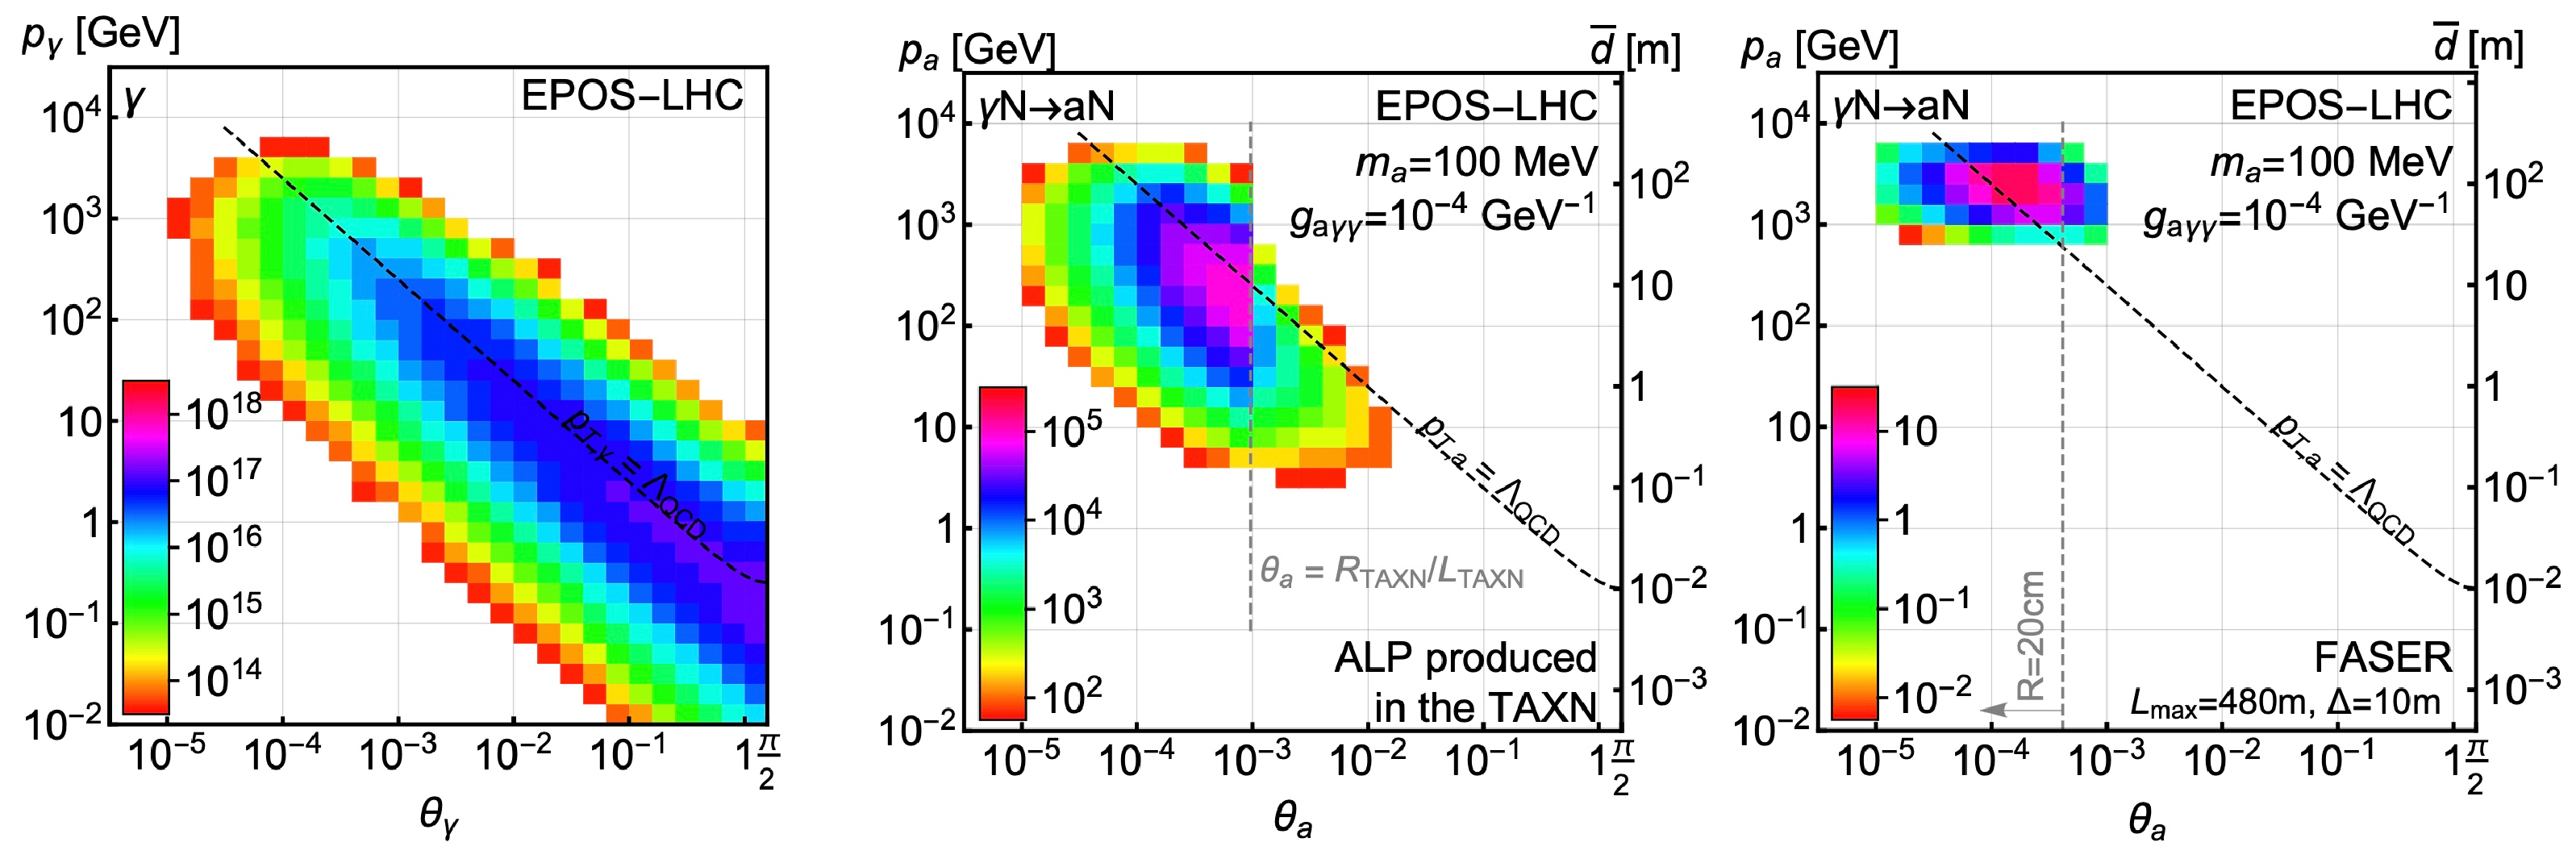
\includegraphics[width=0.95\linewidth]{files/primakoff_prod_TAN}
			\caption{Originating from the photon flux from ATLAS IP (left panel), ALPs can be produced in the TAN (center panel) and later reach FASER and decay (right panel)}
			\label{im:photon_ATLAS_ALP}
		\end{figure}
		
		Once produced, the ALPs will mainly decay into a pair of photons as the decay into fermions pair is suppressed in this reduced model with only photon coupling at leading order. One of the sub-leading decays channel is the one in which the ALP decays into one real and one virtual photon, further decaying into an electron-positron pair with a branching fraction of the order of $\mathcal{B}(a \rightarrow \gamma e^+ \hspace{1mm} e^-) \approx 1 \%$ \cite{FASER_LLP}. For the primary ALP decay channel, the decay width is given by: 
		\begin{equation}
			\Gamma_a(a\rightarrow \gamma \gamma) = \frac{g_{a \gamma\gamma}^2 m_a^3}{64 \pi}
		\end{equation}
		
		The cubic dependence on the mass of the ALP is a consequence of the dimension-5 operator which mediates the di-photon coupling. The decay length of the ALP can then be written as: 
		\begin{equation}
			\bar{d}_a = c \frac{1}{\Gamma_{a}} \gamma_{a} \beta_{a} 
			\label{eq:ALP_decay_length}
		\end{equation}
		
		The ALP decay length, branching fractions into di-photon and sub-leading fermionic channel are shown in the left panel of figure \ref{im:ALP_photon_prod}. The sensitivity reach in the $m_{a}$ and $g_{a\gamma\gamma}$ parameter space for FASER for ALPs produced through Primakoff Process is presented in the right panel of figure \ref{im:ALP_photon_prod} together with a comparison between the already excluded regions (in grey), current and future experiments.
		
		A detailed interpretation of the sensitivity reach presented is given in \cite{FASER_LLP} but is is striking to see that FASER will already be able to probe unconstrained regions with potential discovery in the mass range $m_a  \sim $ 30 - \SI{400}{\mega\electronvolt} throughout the LHC Run 3 \cite{Primakoff_process}. For large couplings to di-photon, the sensitivity reach is constrained by the decay length of the ALP while for lower couplings the lifetime is usually longer as ALPs are less boosted, resulting in a larger emission angle with respect to beam axis for which the geometrical acceptance of the detector becomes the limiting factor \cite{Primakoff_process}. 
		\clearpage	
		
		\begin{figure}[h]
			\centering
			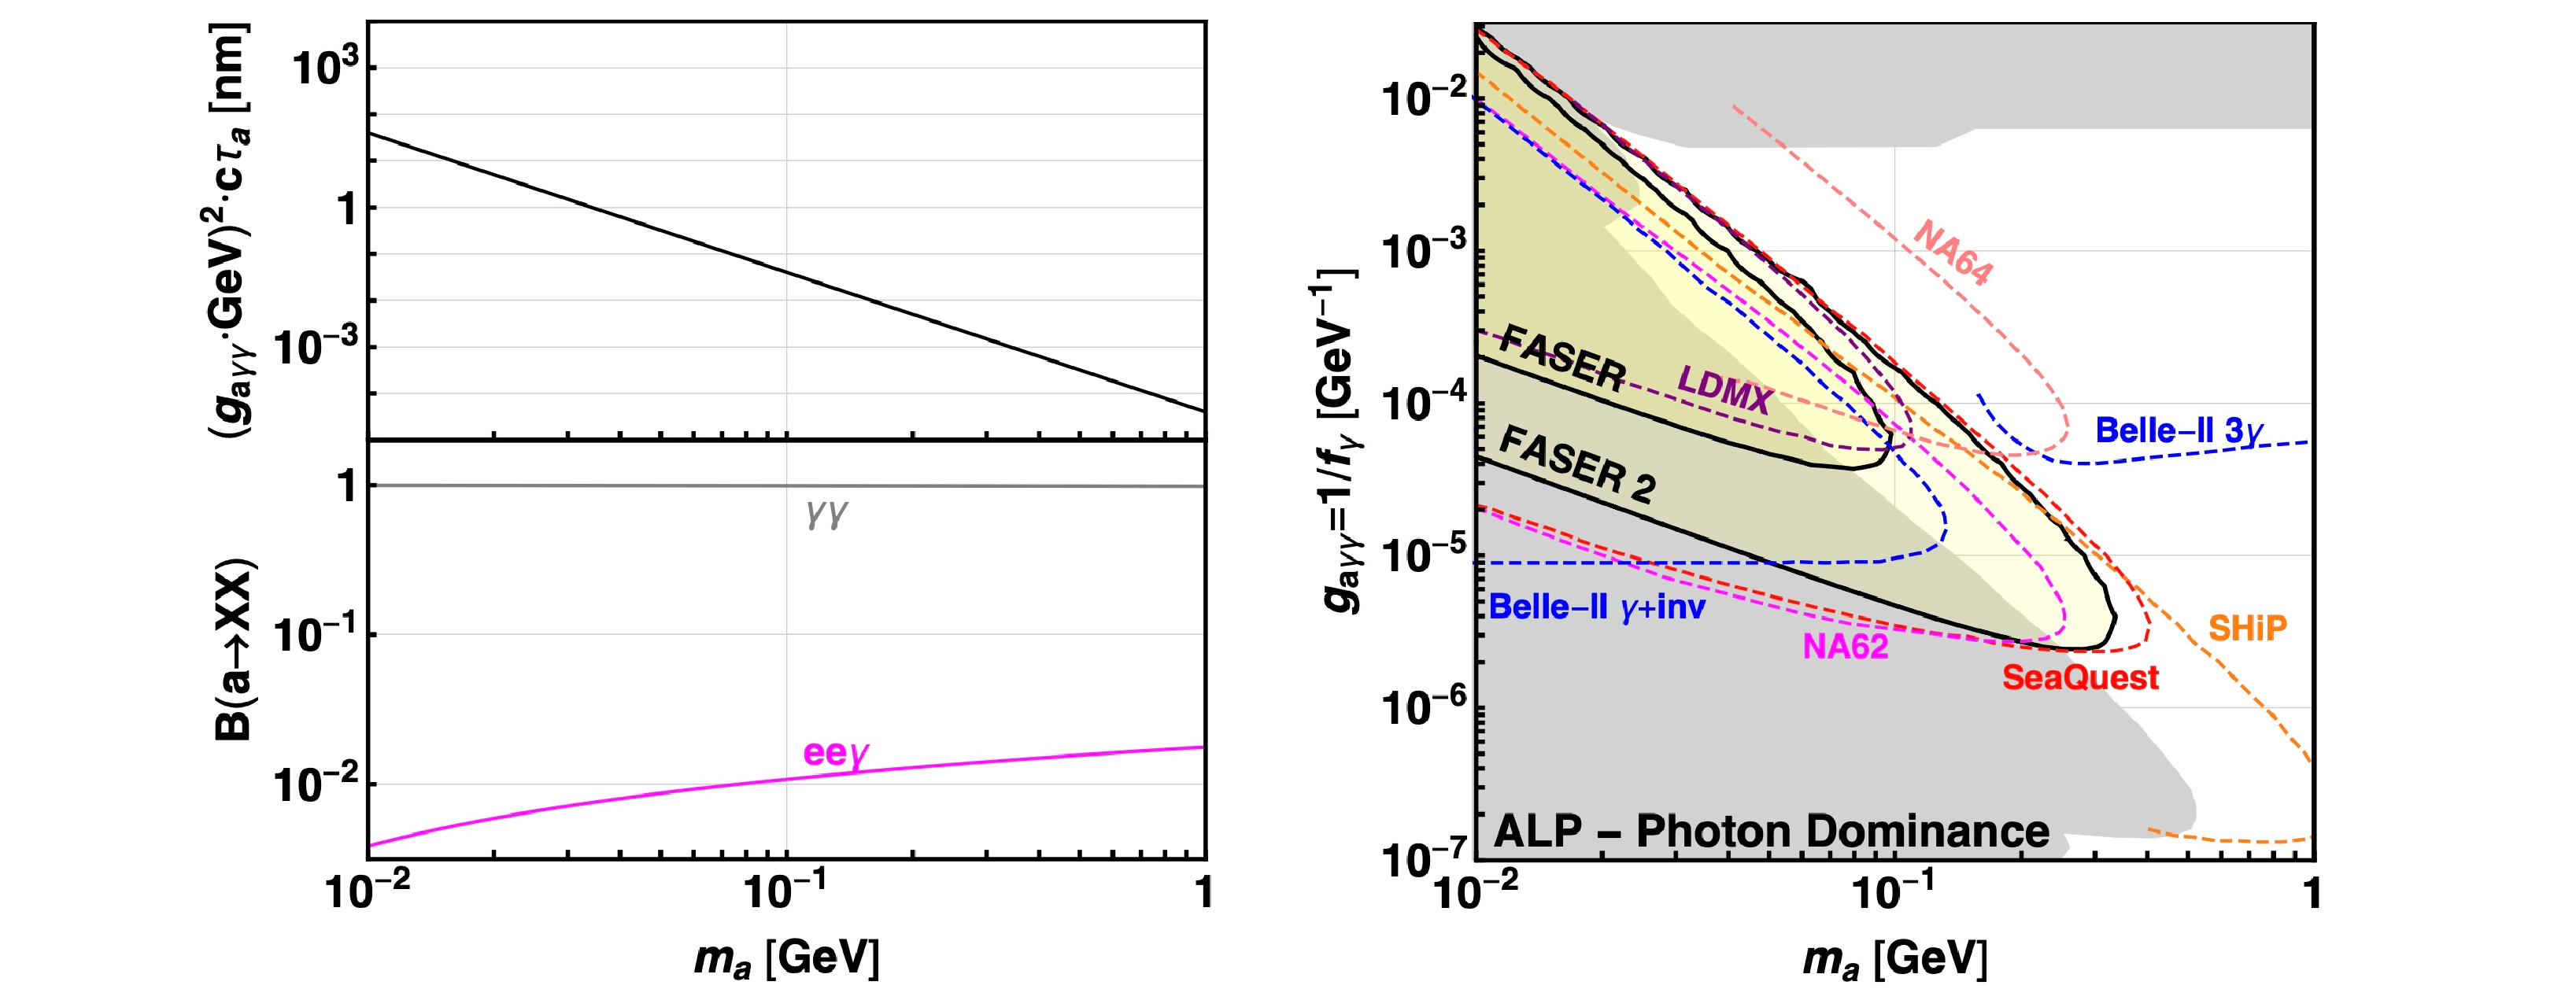
\includegraphics[width=0.9\linewidth]{files/ALP_photon_production}
			\caption{The ALP decay length (top left panel), its branching fractions in diverse possible final states (bottom left panel) and FASER's reach in the ALP parameter space defines by its mass and coupling to di-photons}
			\label{im:ALP_photon_prod}
		\end{figure}
		
			
		\subsection{Neutrinos from collider}
		The special location of the FASER detector doesn't only provide good sensitivity to BSM model but also provides a completely new way of studying neutrinos from collider experiments. The large flux of hadrons in the very forward direction produces through their decay a significant flux of neutrinos highly collimated along the beam axis. All three flavours of neutrinos will be able to reach FASER, if one was to assume a detector with target mass \SI{1.1}{\tonne} (FASER$\nu$) exposed to an integrated luminosity of 150 fb$^{-1}$, the number of neutrinos reaching FASER, undergoing Charged-Current (CC) interactions and their average energy deposition would be those found in Table \ref{tab:neutrinos_flux}.
		\begin{table}[h]
    		\centering
    		\begin{tabular}{|l|c|c|c|}
        		\hline
        		& $\nu_e$ & $\nu_\mu$ & $\nu_\tau$ \\
       		 	\hline
       		 	Dominant production process & $K \to \nu_e e X$ & $\pi \to \nu_\mu \mu$ & $D_s \to \nu_\tau \tau$ \\
        		\hline
        		Number of $\nu$ traversing FASER$\nu$ & $3 \times 10^{11}$ & $2 \times 10^{12}$ & $8 \times 10^{9}$ \\
        		\hline
        		Number of $\nu$ interacting in FASER$\nu$ (1.1 tonnes) & 830 & 4400 & 14 \\
        		\hline
        		Average energy of interacting neutrinos (GeV) & 820 & 820 & 810 \\
        		\hline
    		\end{tabular}
    		\caption{Expected neutrino fluxes, interactions, and average energies at FASER$\nu$ \cite{FASER_Detector}}
    		\label{tab:neutrinos_flux}
		\end{table}  
		
		\begin{figure}[h]
			\centering
			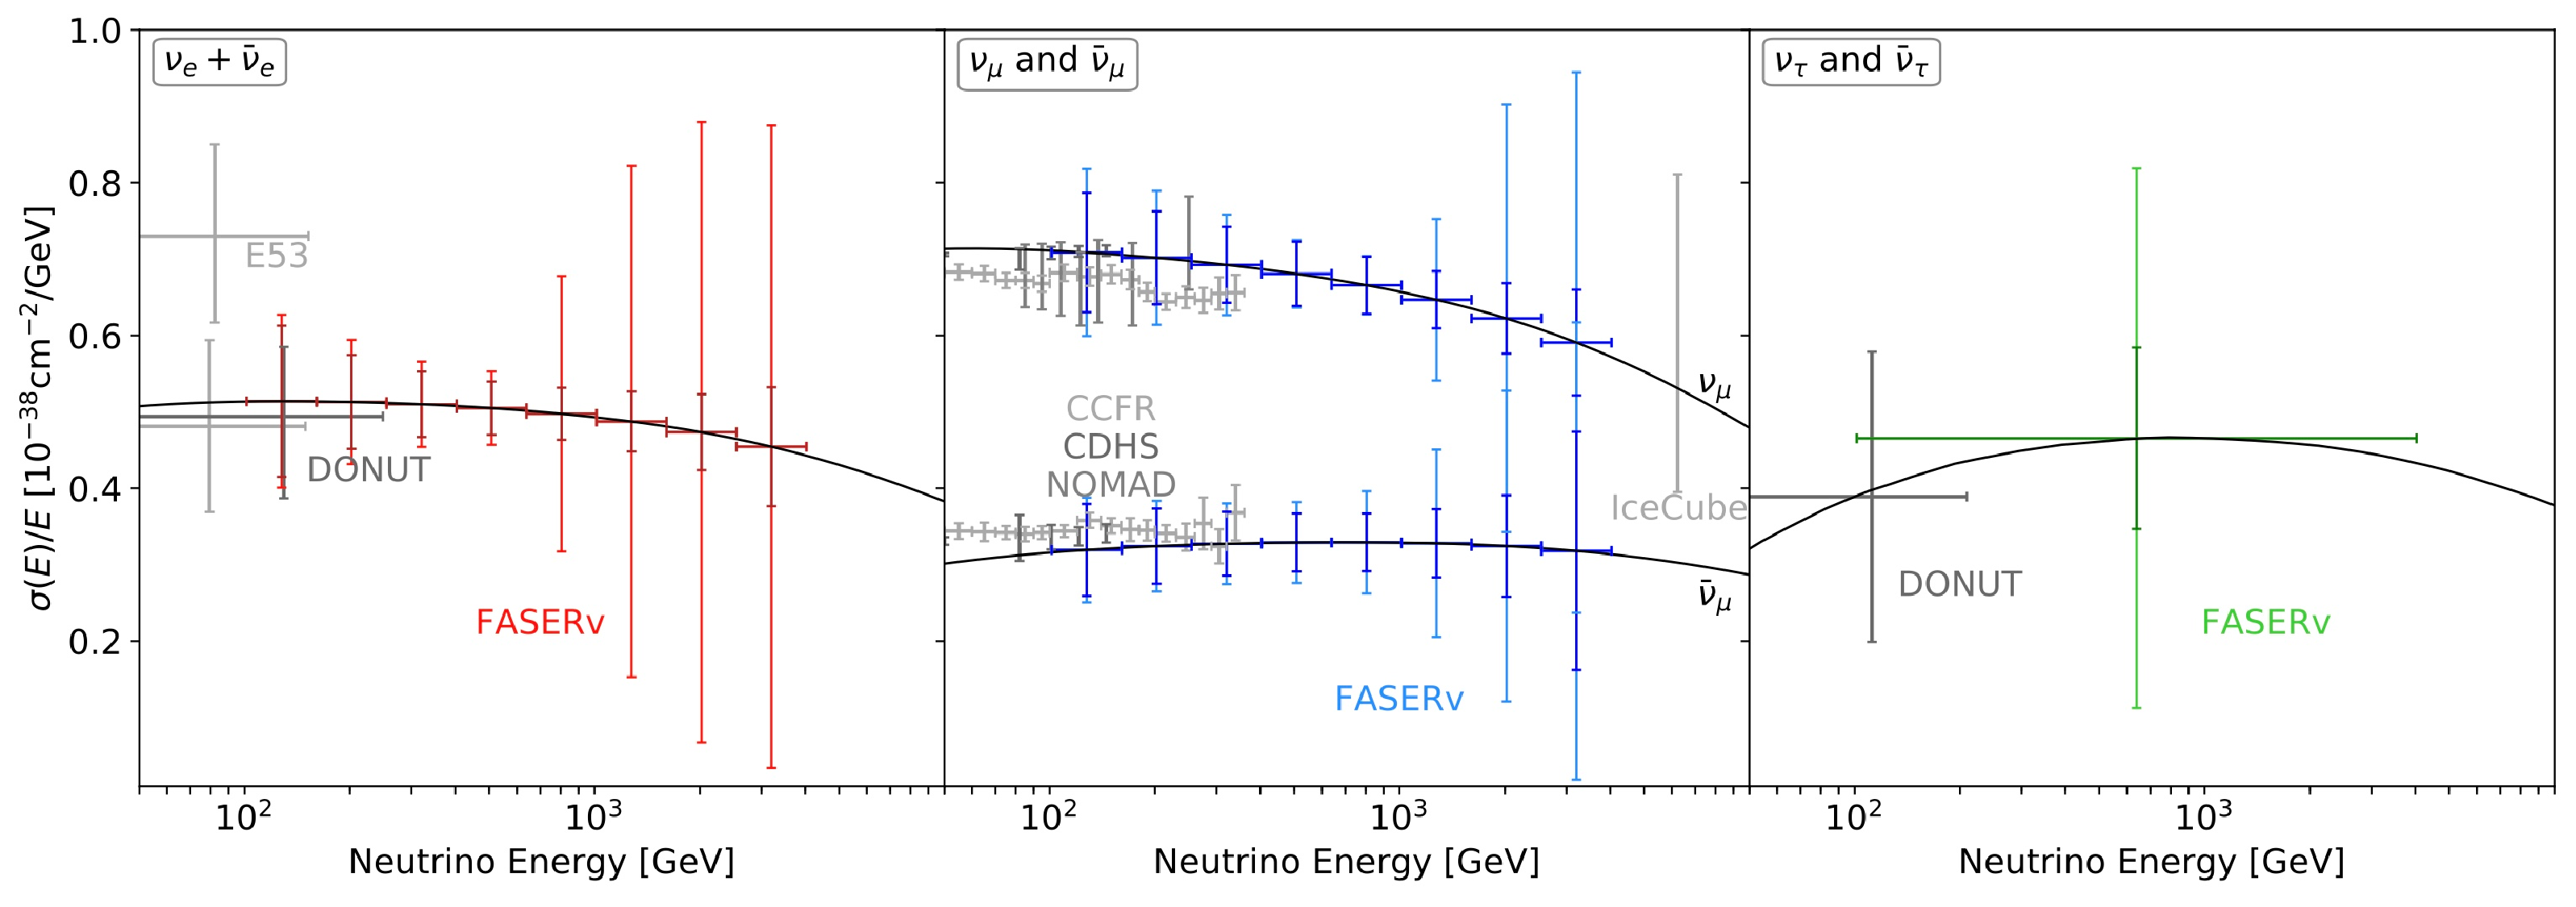
\includegraphics[width=0.845\linewidth]{files/neutrino_XS}
			\caption{FASER$\nu$ estimated CC cross section sensitivity for $\nu_e$ (left), $\nu_\mu$ (center), $\nu_\tau$ (right). The black curve is the theoretical prediction while coloured error bars are statistical uncertainties (inner) and the combination of statistical and flux uncertainties (outer).}
			\label{im:neutrino_XS}
		\end{figure}
		\clearpage
		
		Studying the flux of neutrinos reaching FASER is essential as for now, the theoretical uncertainties on the production of forward hadrons are large. As a matter of fact, varying the generator model in simulations can lead to substantial changes in the neutrino flux \cite{FASER_Detector}. A precise measurement as a function of energy and rapidity will help defining better constrains models for forward hadron production and also many more parameters as explained in detail in \cite{FASER_Detector}.  
		
		The large flux of neutrinos will allow FASER to perform a measure of the CC neutrino cross section at energy regimes not yet studied, the projection on the measurement precision is given in figure \ref{im:neutrino_XS}. The uncertainties are given separately for different generators models. 
		
		As a proof of principle, a small emulsion detector with target mass of \SI{11}{\kilo\gram} was placed along the Line of Sight (LoS) for 4 weeks during the LHC Run 2 in 2018 and recorded the first neutrino interactions candidates at a particle collider \cite{neutrino_pop}
	\clearpage
	
	
	
	\section{The ForwArd Search ExpeRiment}
	 The Physics program of FASER is quite diverse, probing both the SM in yet uncovered regimes and the hidden sector through the SM decay of LLPs originating from SM particles produced in the very forward direction at the ATLAS IP. In order to perform these various measurement, the layout of the FASER detector has to be tuned to provide the best sensitivity to the diverse signal's signatures. 
	 In the following section discussion on the possible backgrounds for the different signatures will be presented, followed by a list of the requirements on the design of the detector. An overview of the chosen layout of the detector and its subcomponents will be presented along with a brief description of the typical signatures from LLPs, shining light on the need for an upgrade of the initial detector layout to further improve sensitivity.   
	
		\subsection{Background from the Standard Model to LLP signals}
	
		Only a limited set of Standard Model particles produced at the IP can penetrate the material separating the ATLAS and FASER, made by approximately \SI{90}{\metre} of rock, concrete, and diverse infrastructures. A detailed studying FLUKA and GEANT4 simulations~\cite{FASER_techprop, FASER_loi} show that only high-energy muons and neutrinos are capable of traversing the shielding material and produce appreciable rates at FASER. The studies were made for the TI18 tunnel (opposite location to TU12 tunnel with respect to ATLAS) but there is a priori no major difference on the results \cite{FASER_techprop}. These particles constitute the dominant potential backgrounds for LLPs searches with FASER.

			\subsubsection{Muon-induced backgrounds}  
			The muons flux is predominantly produced from decay of pions, kaons and other heavy flavour hadrons produced at the ATLAS IP, the pions are mostly coming from collisions debris interacting with the LHC infrastructure such as the TAN neutral absorber. \cite{FASER_Detector}. A sub-leading source of muons actually come from the ATLAS IP itself but only account for a few percent of the total flux \cite{FASER_techprop}. The results from the FLUKA simulations predict a peak muon fluence at FASER around $\sim$ \SI{100}{\giga\electronvolt} as show in figure \ref{im:muon_flux}.
		
			\begin{figure}[h]
				\centering
				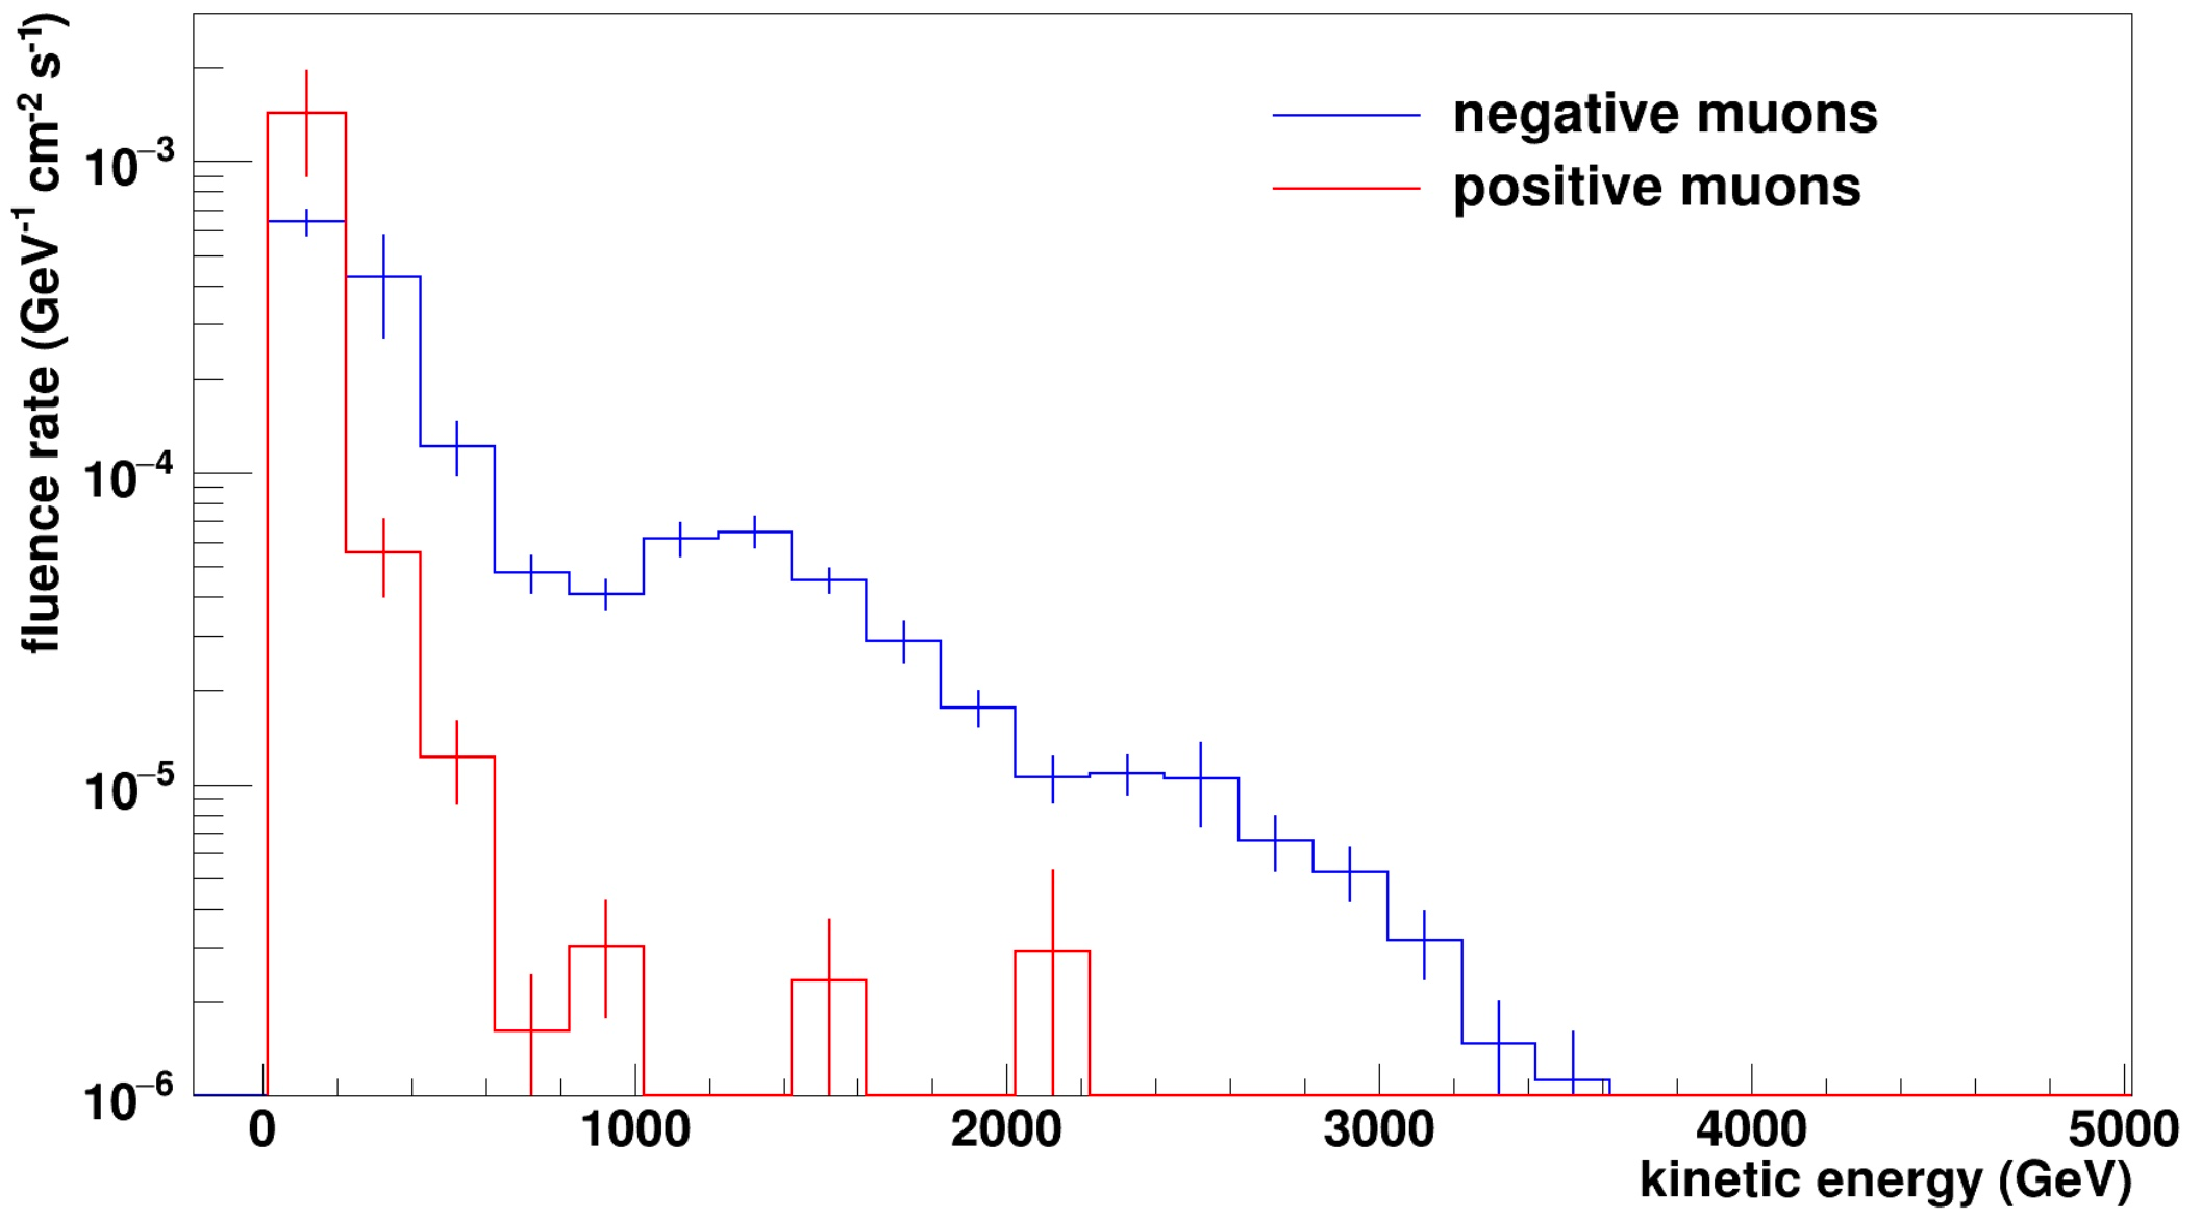
\includegraphics[width=0.8\linewidth]{files/muon_flux}
				\caption{FLUKA simulations estimations of the muon flux as a function of the energy. The flux is given separately for $\mu^+$ (in red) and $\mu^-$ (in blue). The flux is normalised to a luminosity of $2 \times 10^{34}$ cm$^{-2}$ s$^{-1}$}
				\label{im:muon_flux}
			\end{figure}
			
			The flux for $\mu^+$ and $\mu^-$ is very different due to the due to the bending of the magnets from the LHC. For particles above \SI{10}{\giga\electronvolt} the muon traversal rate per surface unit is of the order of \SI{0.5}{\hertz\centi\meter}$^{-2}$. The particles produced by interaction of the neutrinos in the material have not been taken into account as their contribution is several order of magnitude lower. The location of FASER is very strategic as it sits in a region where the muon flux is particularly low with respect to surrounding areas (within \SI{2}{\meter}) as show in \cite{FASER_techprop}.\\

			The copious amount of muons reaching FASER could produce signatures mimicking those of the decay of an LLP in the following ways:  
			\begin{itemize}
    			\item \textbf{Hard Bremsstrahlung:} A high-energy muon can emit a bremsstrahlung photon in the detector material, producing an $e^+e^-$ pair and mimicking an electromagnetic LLP decay such as the one of the dark photon. If the muon was to produce two consecutive photons, highly collimated and not converting in the detector material, this could also lead to a fake di-photon ALP signature. 
    			\item \textbf{Direct Pair Production:} Muons can directly produce $e^+e^-$ pairs via interactions in the detector, also faking a displaced electromagnetic vertex for the dark photon.
    			\item \textbf{Muon Catastrophic Energy Loss:} Rare catastrophic losses can deposit significant energy, appearing as highly energetic showers.
			\end{itemize}
		
			\subsubsection{Neutrino-induced backgrounds}  
			Neutrinos in the forward direction are predominantly produced in the decays of hadrons which can either occur at the IP itself or further down the beam pipe and travel essentially unimpeded to FASER. The neutrino energy spectrum extends from a few GeV up to several TeV as shown in figure \ref{im:neutrino_flux}.
			\begin{figure}[h]
				\centering
				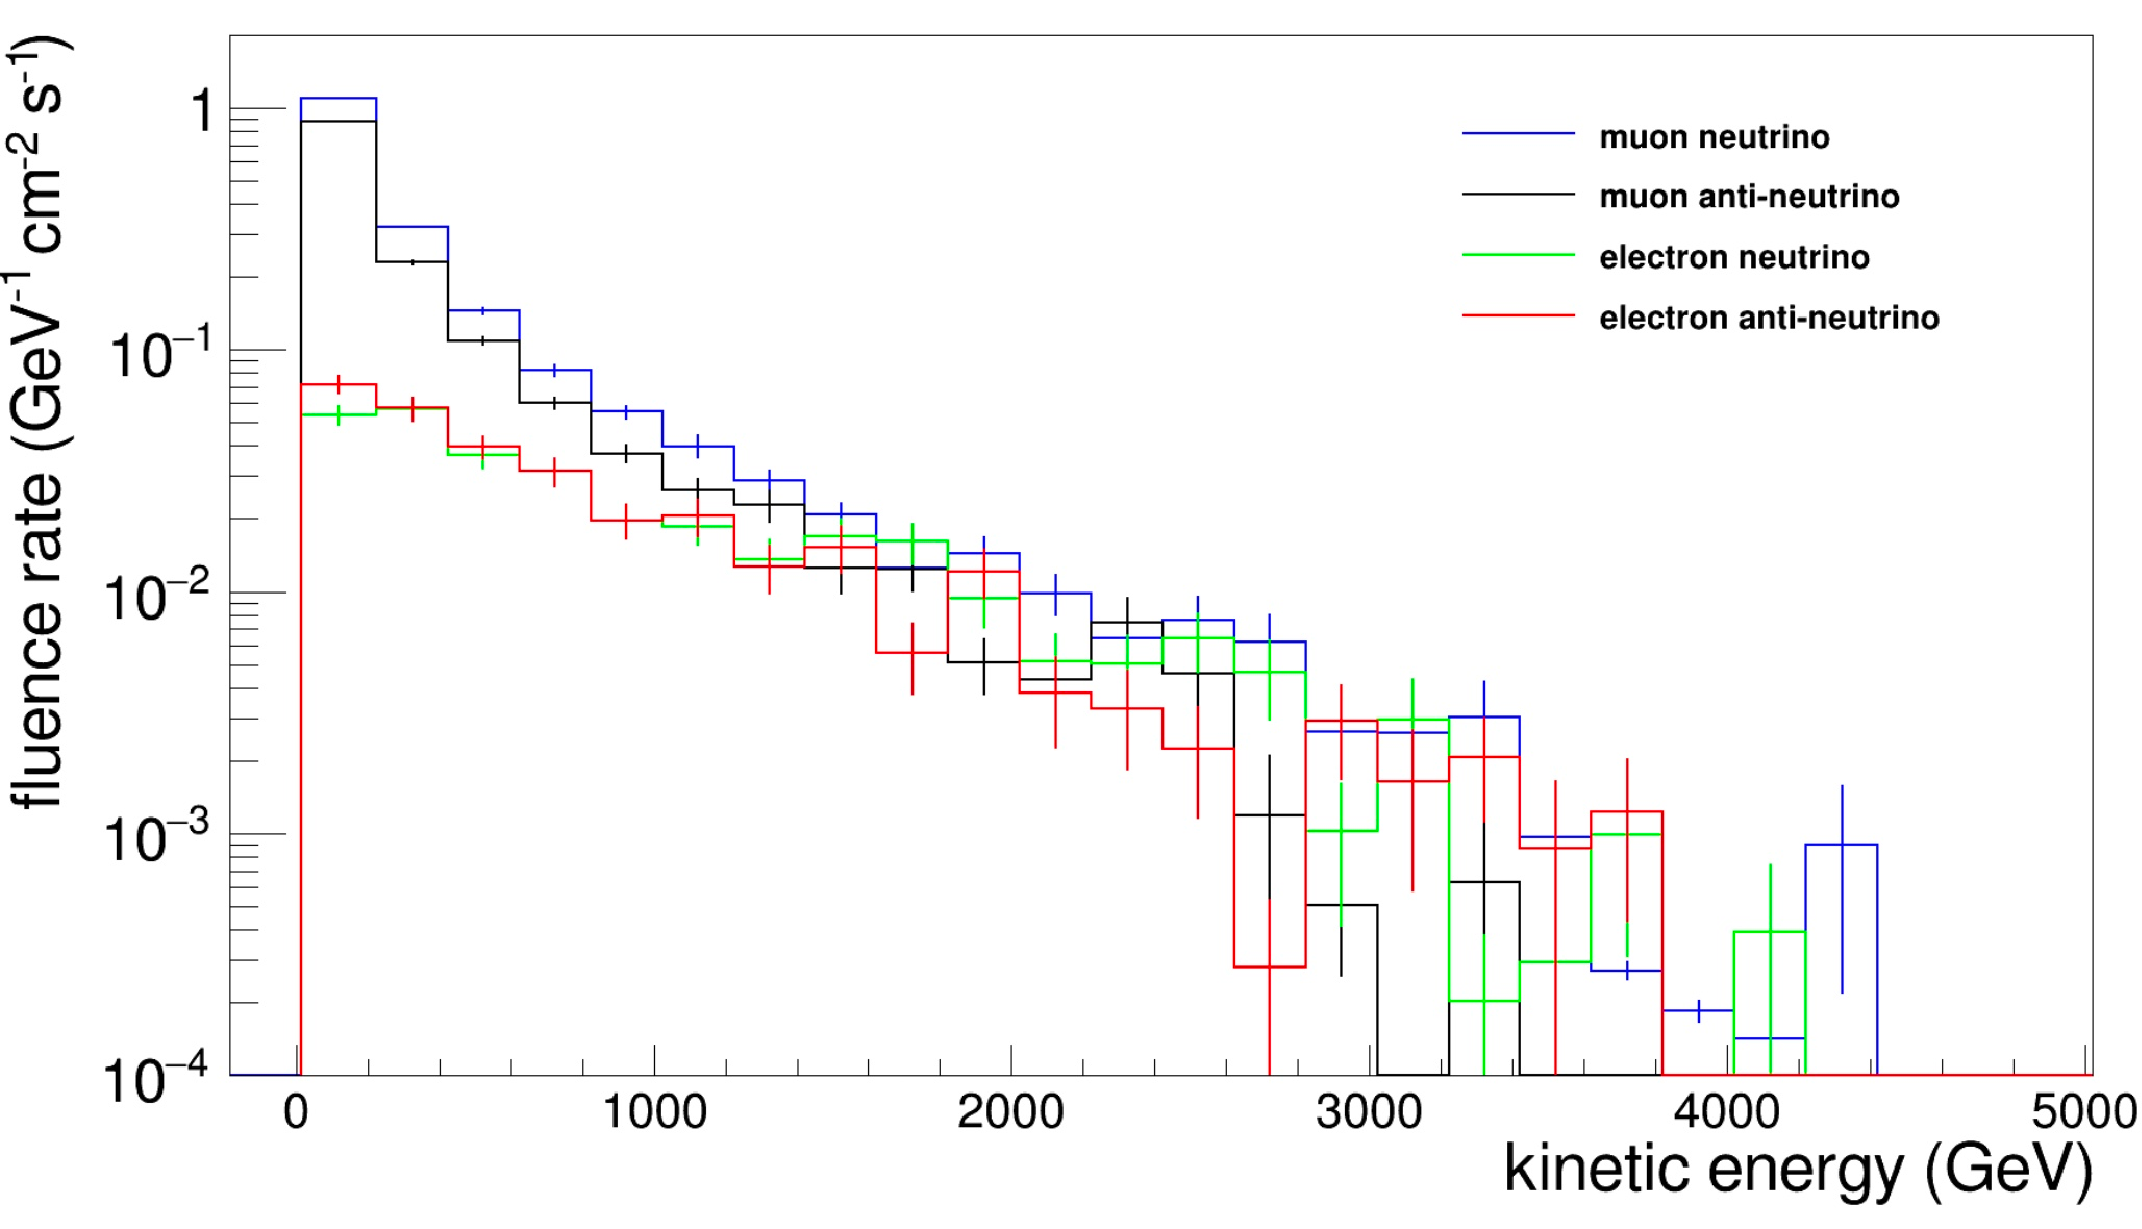
\includegraphics[width=0.8\linewidth]{files/neutrino_flux}
				\caption{FLUKA simulations estimations of the neutrino flux as a function of the energy. The flux is given separately for $\nu_{e}$ (in red) $\nu_{\mu}$ (in blue) $\bar{\nu}_{\mu}$ (in black) and $\nu_{\tau}$ (in green). The flux is normalised to a luminosity of $2 \times 10^{34}$ cm$^{-2}$ s$^{-1}$}
				\label{im:neutrino_flux}
			\end{figure}

			Neutrino CC interactions inside the detector can mimic LLP decays by producing visible final-state charged leptons or hadronic activity emerging from a seemingly empty region. However, neutrino interaction rates are drastically suppressed by their small cross section.
			While irreducible in principle, the neutrino-induced background remains extremely small compared to potential LLP signals.

		\subsubsection{Beam-induced backgrounds}  
		Additional backgrounds could arise from beam-gas interactions (collisions between LHC protons and residual gas molecules) or beam losses in the accelerator infrastructure. GEANT4-based studies including measured vacuum conditions demonstrate that such backgrounds are suppressed by several orders of magnitude relative to the muon flux and are negligible~\cite{FASER_techprop}.


		\subsubsection{Validation with in situ measurements}  
		During Run 2, emulsion-film detectors installed on the beam collision axis in TI12 measured the charged-particle fluence directly. The observed flux of $(1.2-1.9)\times10^4$~cm$^{-2}$~fb$^{-1}$ within \SI{10}{\milli\radian} matches simulation predictions \cite{FASER_techprop}. These measurements confirm the FLUKA modelling of particle fluxes at FASER’s location and validate that no unexpected backgrounds are present. A complementary measurement with a TimePix beam-loss monitoring system shows a correlation between the rate of charged particles and the ATLAS luminosity as expected from the FLUKA simulations. \\
		
		This overview of the different source of background from the SM to LLP decay signatures imposes new constraints on the layout of the detector in order to be able to nicely separate signals from and beyond the Standard Model. 
		
		\subsection{Detector requirements}
		
		In order for FASER to fully exploit its physics program on the hidden sector and neutrino cross section measurements, a specific set or requirements on the layout of the detector are imposed. The distinction from SM induced signatures and pure LLP decay signatures must also guide the design of the detector. An overview of the most relevant requirements on the FASER detector is presented below. 
		
		\subsubsection{Position within TI12 tunnel}
		The FASER detector must be precisely aligned on the ATLAS LoS to within \(\pm10\)\,cm for all beam–crossing angles, in order to maximise both the acceptance of LLP signatures and the energy of neutrinos traversing the active volume. \cite{FASER_Detector}. In order to suppress the large background of high‐energy muons produced at the ATLAS IP, the detector must include a veto system for charged particles entering the detector with an inefficiency smaller than $10^{-9}$ since the expected number of muons entering FASER throughout Run 3 is estimated to me $\mathcal{O}(10^9)$ \cite{FASER_Detector}.
		
		\subsubsection{Energy and Momentum measurements}
		A tracker for high-energy charged particle with good spatial precision is essential in the design of the detector. For a dark photon with mass $m_{A'} =$ \SI{100}{\mega\electronvolt} reaching FASER with a momentum of \SI{2}{\tera\electronvolt}, the expected opening angle of the decay products is $\sim $ \SI{50}{\micro\radian}. A magnet with consequently designed bending power needs to be able to separate the opposite charged tracks of highly boosted LLP decays up to measurable distance by the tracker. The tracker together with the magnet is often referred to as the tracking spectrometer. It is also required to be able to measure the charge of the muons produced in $\nu_{\mu}$ and $\bar{\nu}_{\mu}$ interactions, up to a momentum of several hundreds \SI{100}{\giga\electronvolt}.
		
		To complement the momentum measurement of the spectrometer, an electromagnetic calorimeter is placed downstream. Capacity of measuring TeV‐scale energy deposits with a few‐percent resolution is required to reconstruct e\(^{+}\)e\(^{-}\) or \(\gamma\gamma\) final states from dark‐sector decays such as dark photon or ALPs.
		
		\subsubsection{Large target mass detector for neutrinos}
		Within the tight spatial constraints of the TI12 tunnel, a compact, high‐density neutrino target is needed to collect a sufficient amount of CC interactions. The detector must be able to identify muons, electrons (and distinguish them from gamma rays), and identify short‐lived \(\tau\) and charm decays through a combination of passive material, finely‐segmented active layers, and excellent vertex and angular resolution.  A precision tracker immediately downstream of the emulsion‐based system facilitates the matching of tracks between the passive and active elements, reducing combinatorial ambiguities by $\mathcal{O}(10^{6})$ via a scintillator veto on front‐stack triggers \cite{FASER_Detector}.
		
		
		\subsubsection{Trigger and Data acquisition}
		The trigger and data‐acquisition system must operate robustly at a muon‐induced rate of $\mathcal{O}(650\,\mathrm{Hz})$ for a luminosity of $2\times10^{34}\,\mathrm{cm}^{-2}\mathrm{s}^{-1}$, with minimal dead time to ensure high efficiency for rare events. Finally, FLUKA simulations and 2018 BatMon measurements predict a low‐radiation environment annual doses below $5\times10^{-3}\,\mathrm{Gy}$ and neutron fluence below $5\times10^{7}\,\mathrm{cm}^{-2}$ allowing the use of conventional (non–radiation‐hard) electronics.
 

		\subsection{Original detector layout}
		
		Once the physics program of the FASER detector was defined, a careful study of the typical decay channels of most prominent LLP model, together with possible signals from high energy collider neutrinos shaped its layout. To minimise other SM signals altering the sensitivity of very rare BSM events in FASER, complementary requirements helped defining the detector layout as it will be presented in figure \ref{im:FASER_layout}.
			\begin{figure}[h]
				\centering
				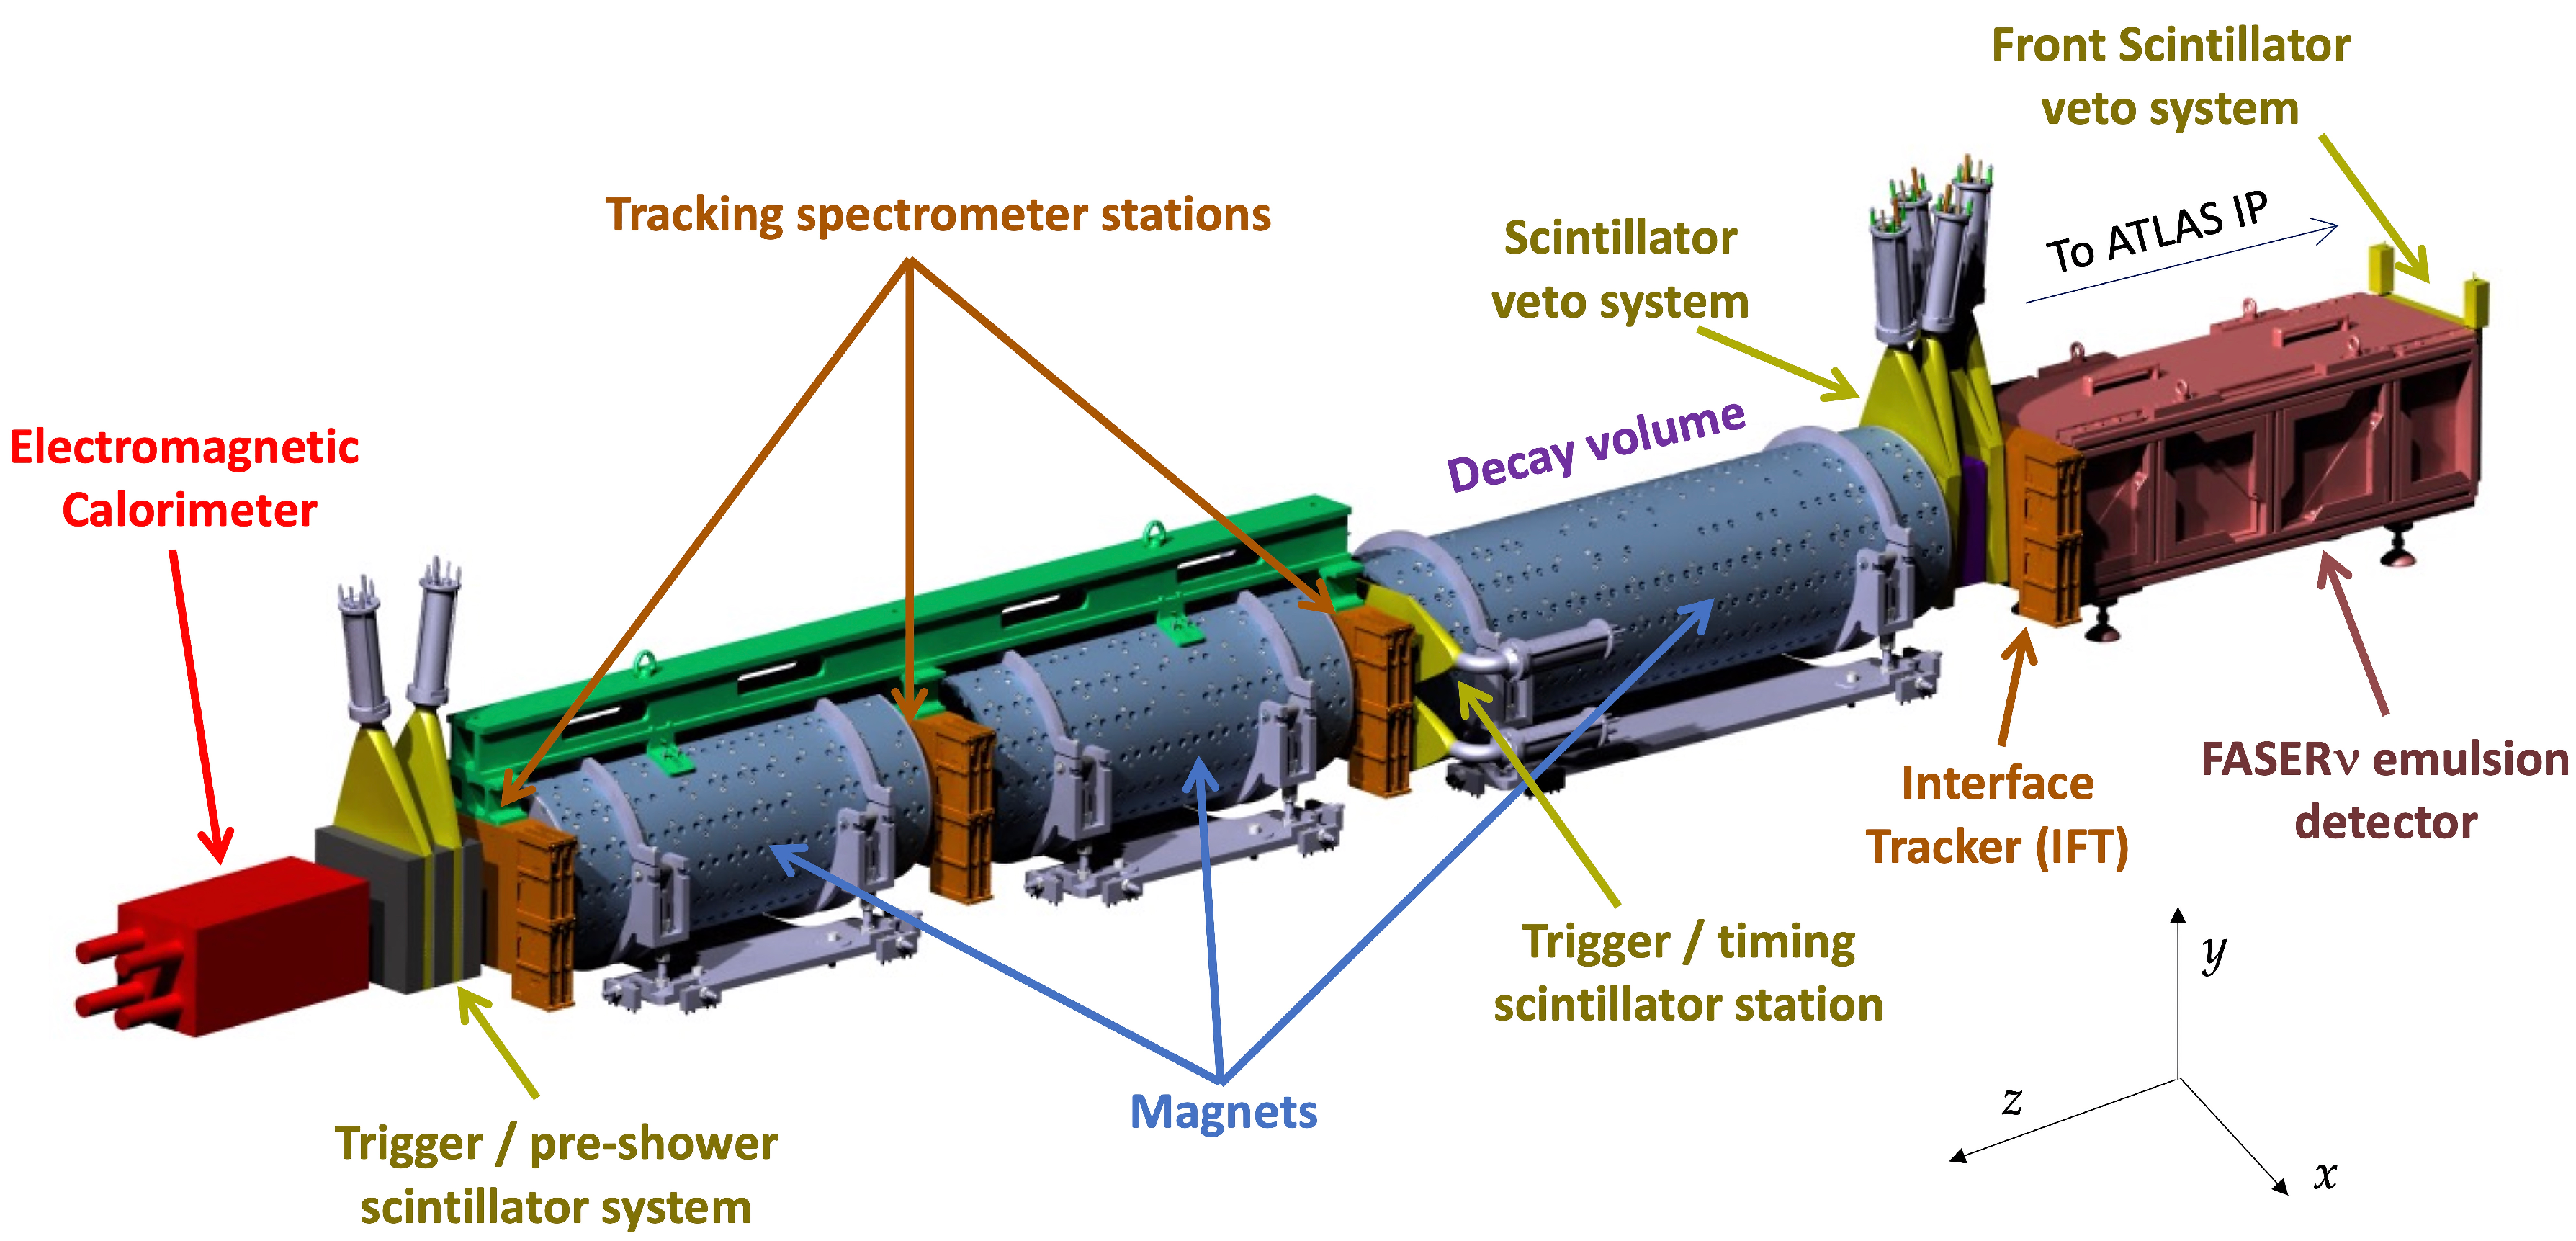
\includegraphics[width=0.9\linewidth]{files/FASER_layout}
				\caption{Layout of the FASER detector with the addition of the FASER$\nu$ detector.}
				\label{im:FASER_layout}
			\end{figure}
			
		Other factors such as short available time for design, construction, commissioning and installation motivated the used of already existing detector components. This helped reducing the cost of the detector while minimising the services and installation works required. The detector can be separated into different modules, each of them having one or more purposes and often acting as a whole, both for event reconstruction and vetoing. 
		
			\subsubsection{The magnet system}
			One of the key elements of the FASER detector is the set of three dipole magnets producing a \SI{0.57}{\tesla} magnetic field inside the decay volume and the tracking spectrometer. Permanent magnets were specifically chosen and designed for the detector, aiming at a reduced amount of services required for operation. The magnets have a \SI{20}{\centi\meter} aperture at the center and their outer radius extends to \SI{43}{\centi\meter}, the first magnet is part of the decay volume and is \SI{1.5}{\meter} long while the other two magnets are part of the tracking spectrometer and are both \SI{1.0}{\meter} long. 
				
			The aim of having magnets is the ability to separate the tracks of charged decay products, mainly the electron-positron pair (or more rare muon anti-muon pair) coming from a Dark Photon decay. The system is also tasked with measuring the charge of muons produced in neutrinos interactions. The magnetic field outside of the magnet should be as small as possible in order not to affect the readout of other detector subcomponents such as PhotoMultiplier Tubes (PMTs). 
		
			\subsubsection{The tracking system}
			The tracking system of the FASER detector can be divided into two separate systems: the Interface Tracker (IFT) and the tracking spectrometer. The IFT is a single tracking station located right after the FASER$\nu$ emulsions detector where as the tracking spectrometer is composed of three tracking stations located at the end of each dipole magnet (see figure \ref{im:FASER_layout}). 
			
			The IFT and tracking spectrometer operate synergistically. The tracking spectrometer is tasked with the reconstruction of the trajectories of charged particles crossing the detector. It provides both a position and momentum measurement and can also identify the charge of muons arising from neutrino interactions. The IFT provides a matching between the tracks reconstructed in the emulsion detector and the tracks registered in the active detectors \cite{FASER_Detector}. A timestamp can be associated to reconstructed tracks in the emulsion detector from neutrino interaction, hence using the tracking system information for muon identification. The information from the rest of the detector can further be used for background rejection and better reconstruction of the neutrino energy \cite{FASER_Detector}. 
			
			The two systems consist of three double-layers of single sided silicon microstrip detectors. Each layer is made of eight silicon strip modules and are spares from the ATLAS experiment's SCT barrel detector \cite{SCT_ATLAS}. Each SCT module cover an area of $6 \times 12$ cm$^2$ and they are arranged in 2 columns made of 4 modules to cover a total active area of $24 \times 24$  cm$^2$, hence covering the full aperture of the magnets. The SCT modules are made of two silicon layers, assembled with a small stereo angle of \SI{40}{\milli\radian} providing a \SI{20}{\micro\meter} resolution in the bending plane and \SI{800}{\micro\meter} otherwise. In terms of performances the tracking spectrometer have a well above 99 $\%$ detection efficiency (per SCT module) and is able to distinguish particles tracks separated by $100-200$ $\mu$m. The IFT is capable of providing a track angular resolution  of \SI{250}{\micro\radian} in the bending plane and \SI{13}{\milli\radian} otherwise.  
			  
			 \subsubsection{The Scintillator and calorimeter systems}
			 The detector is instrumented with four different scintillator stations contributing both to vetoing unwanted background events and triggering. These stations are placed before and after the FASER$\nu$ emulsion detector and on both ends of the tracking spectrometer (see figure \ref{im:FASER_layout}). The electromagnetic calorimeter is placed right after the last scintillator station. Its purpose is to measure the energy of high-energy electrons and photon and also take part in triggering for signals with large energy deposition. 
			 
			 The first two stations are essential in assessing whether or not a charged particles entered the detector. The station in front of the FASER$\nu$ emulsion detector is made of two scintillator counter while the second station is made of four scintillator counters. Each scintillator is read out by a dedicated PMT. The scintillator cover a larger area that the aperture of the magnets, this helps with vetoing charged particles entering FASER with an angle, their inefficiency has to be compatible with the high muon rate expected on their full active area. 
			 
			 The third scintillator station, also known as the timing station is made of two scintillator counters and are each read out by two PMT on each side in the transverse plane. This station detect whether or not charged particles enter the tracking spectrometer and assigns a precise time for triggered events (with a resolution better than \SI{1}{\nano\second}) \cite{FASER_Detector}.
			 
			 The fourth and last scintillator station, also known as the pre-shower station is composed of two scintillator counters, readout by a single PMT. Each scintillator in the station is preceded by a \SI{3}{\milli\meter} thick layer of tungsten and a graphite layer to reduce backsplash from the calorimeter is placed between right after the second scintillator counter. The aim of the pre-shower in this configuration is to help distinguishing between neutrino and photon events in the calorimeter. 
			 
			 Finally, the electromagnetic calorimeter  The station is made of a squared arrangement of four spare modules from the LHCB experiment's outer electromagnetic calorimeter (ECAL) \cite{FASER_Detector}. The sampled design of 66 interleaved layer of lead and plastic scintillator with wavelength shifting fiber driving the collected light to a PMT at the back of each module, offers a total of 25 radiation length and provides an energy measurement with a precision at the percent level in the energy regime needed. It unfortunately offers no transversal position measurement and is unable to distinguish separate two particle tracks. 
			 
			 \subsubsection{The FASER$\nu$ emulsion detector}
			 Initially not in the very first detector layout presented in \cite{FASER_loi, FASER_techprop}, the FASER$\nu$ emulsion detector was added at the very front of the FASER detector to study high energy neutrinos produced in colliders. The detector weights a total of \SI{1.1}{\tonne} and is made of 770 interleaved layers of 1-mm thick tungsten plates for neutrino to interact and emulsion films recording the tracks of charged particles  with excellent position and angular resolution \cite{FASER_Detector}. Oppositely to the rest of the FASER detector, the emulsion detector is passive and readout of the information recorded by the emulsion films requires extraction development and scans of each film before reconstruction of the particle trajectories. 
			 
			 The detector essentially detects neutrinos CC interactions through the identification of the lepton track associated to the vertex. A detailed explanation of how different neutrinos interactions of different flavours can be identified is given in \cite{FASER_Detector}. Since the detector record every charged particle crossing its volume, the track resolution allows for a multiplicity of the order of $\mathcal{O}(10^6)$ per cm$^2$ before it needs to be replaced, which is equivalent to an exposure to $30$-$50$ fb$^{-1}$ of collision data \cite{FASER_Detector}. 
			 
			 \subsubsection{Trigger and Data Acquisition}
			 
			 As previously anticipated, the FASER detector is triggered by any signal in any of the scintillator stations or the calorimeter. The trigger rate essentially comes from muons around the LOS, for the aperture of the magnet, the rate would be \SI{150}{\hertz} but since the scintillator stations were designed with a larger acceptance that the aperture ($40\times 40$ cm$^2$) the expected rate rises to \SI{650}{\hertz}. A schematic and simplified view of the FASER Trigger and Data Acquisition (TDAQ) architecture is given in figure \ref{im:FASER_TDAQ}.
			 \begin{figure}[h]
				\centering
				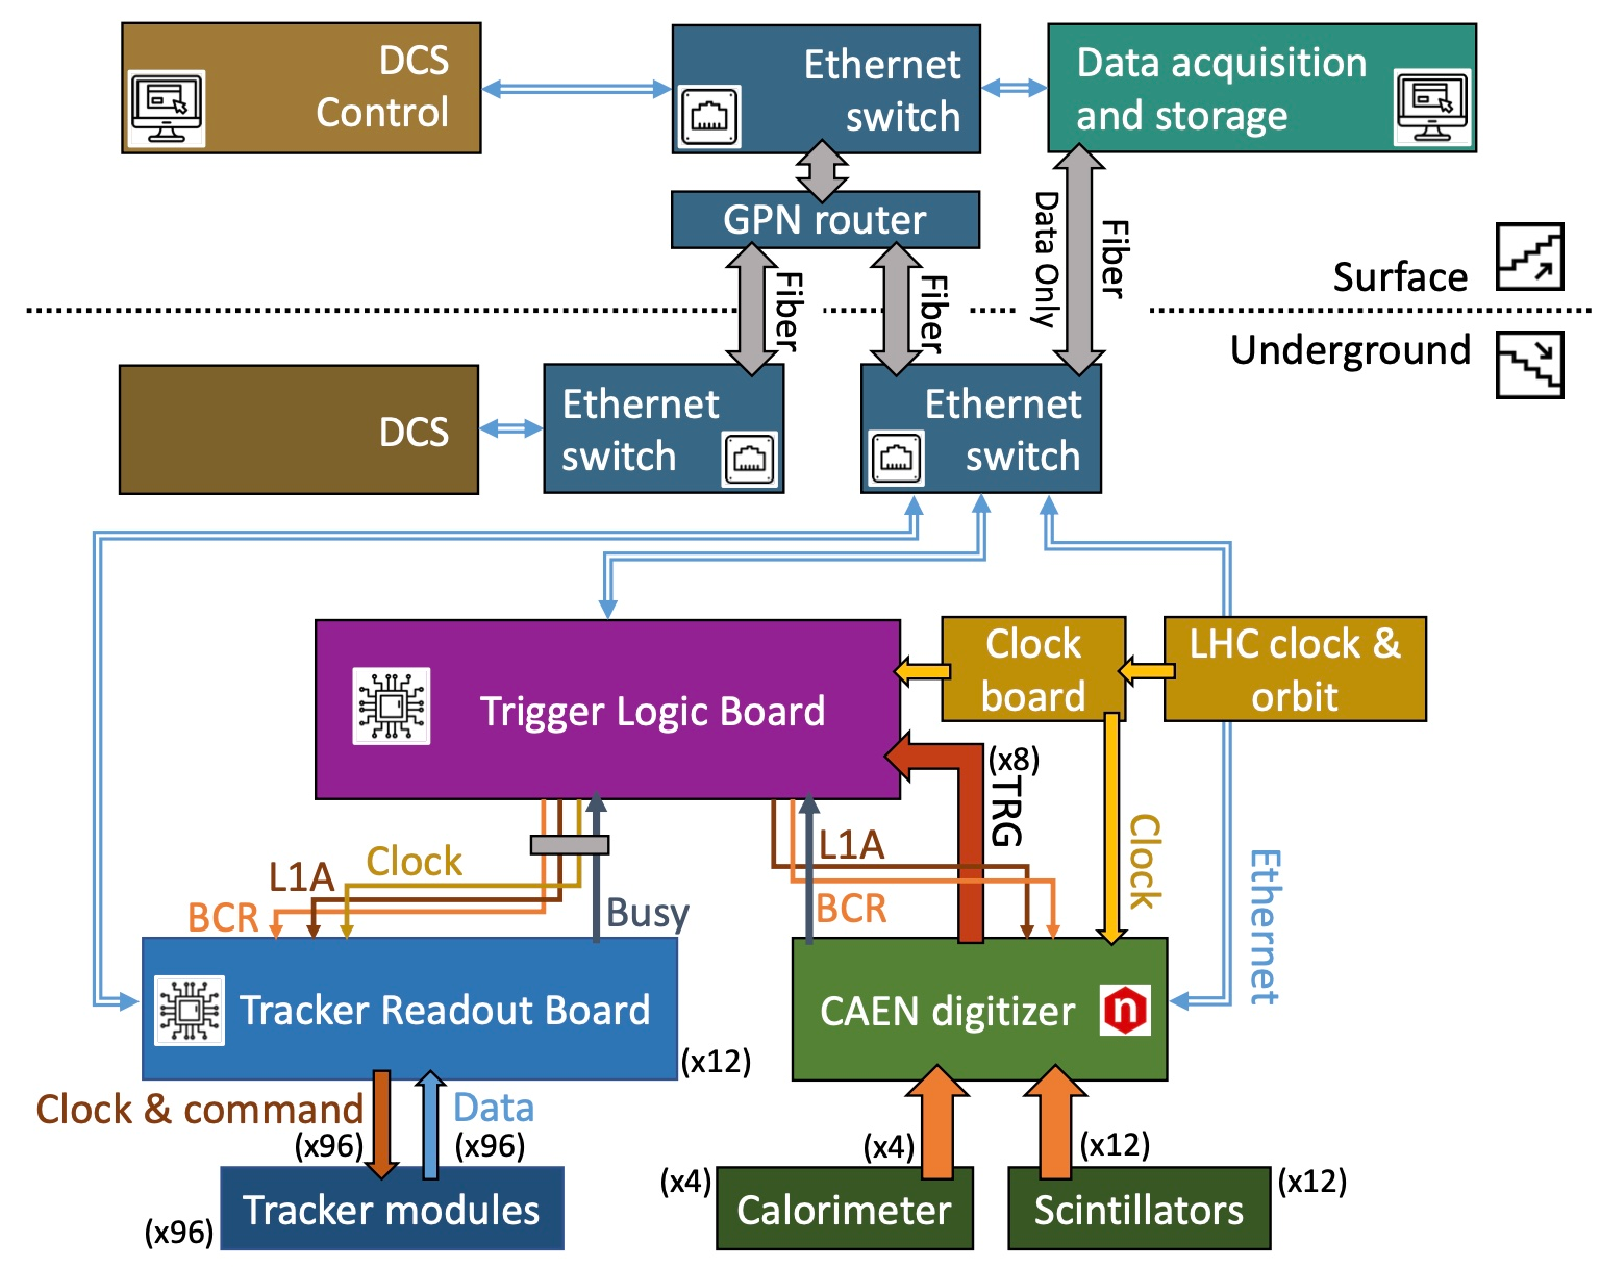
\includegraphics[width=0.8\linewidth]{files/FASER_TDAQ}
				\caption{Schema of the FASER TDAQ architecture. The number in parentheses indicate the number of channels or lines \cite{FASER_Detector}.}
				\label{im:FASER_TDAQ}
			\end{figure}	 
			
			The raw signals from the PMTs of all four calorimeters modules and the tracking stations (for a total of 12 channels) are sent to a commercial digitizer with a pre-defined threshold. The output trigger signal is sent to a custom Field Programmable Gate Array (FPGA)-based Trigger Logic Board (TLB), combining the inputs to form a global trigger, called Level 1 Accept (L1A) trigger. The TLB is able to pre-scale and inhibits certains trigger, it also offers the possibility to do monitoring. Once generated, the L1A signal is sent to the Tracker Readout Boards (TRBs) and the digitizer for initiating the readout of the detector data. A dedicated optical fiber network is in charge of transferring data sent by the readout boards to a software event builder DAQ running on a surface-located server. The TDAQ system's hardware operates at the LHC clock of $\sim$\SI{40}{\mega\hertz}, received and processed via dedicated electronics to correct for jitter and phase shifts throughout running \cite{FASER_Detector}. 
			 
		\subsection{Charged and neutral decay signatures from LLPs}
		The layout fo the FASER detector defined, it is interesting to study the different signatures of the typical LLP decay FASER could observe. Two signatures were previously identified, namely for the dark photon, a decay into a pair of oppositely charged leptons, mostly an $e^+ \hspace{1mm} e^-$ pair and for the ALP a pair of photons. \\ 
		
		The typical signature for a dark photon decay into a lepton pair is presented in figure \ref{im:FASER_OLD_DP_signature}: 
		\begin{figure}[h]
			\centering
			\includegraphics[width=1.0\linewidth]{files/FASER_DP_signature}
			\caption{Typical signature of a dark photon decaying into a pair of oppositely charged leptons ($e^+ \hspace{1mm} e^-$ in this scenario).}
			\label{im:FASER_OLD_DP_signature}
		\end{figure}	
		
		The  decay of a dark photon is hence associated to no signal in the vetoing elements, any signal recorded would indicate a charged particle entering FASER and possibly mimicking an LLP decay signal. Once produced, the oppositely charged lepton pair will be separated by the Lorentz force acting on them, the further down they'll move in the tracking spectrometer, the more they'll separate. It is essential to be able to distinguish the pair of leptons and measure their deviation due to the magnetic field as the precise position measurement offered by the tracking stations in the bending plane allow for a measurement of the momentum of each lepton. Finally, the pair should deposit energy both in the Pre-Shower and the Calorimeter systems, hence providing a measurement of the energy of the lepton pair and hence the dark photon.
		
		The typical signature for an Axion-Like Particle decaying into a photon pair is presented in figure \ref{im:FASER_OLD_ALP_signature}: 
		\begin{figure}[h]
			\centering
			\includegraphics[width=1.0\linewidth]{files/FASER_ALP_signature}
			\caption{Typical signature of an ALP decaying into a pair of photons.}
			\label{im:FASER_OLD_ALP_signature}
		\end{figure}
	
		Similarly, there should be no signal registered in the element of the detector contributing to vetoing. The ALP should decay, leave no presence of its passage through the tracking stations (unless interaction with the tracker material occurs but is very unlikely). A deposit of energy should be recorded in both the Pre-Shower and the Calorimeter systems, signals the presence of at least one photon produced inside the FASER detector. It is important to notice that in this case, the signal for one photon or more than one photo, highly collimated (as suggested if they were originating from the decay of a highly boosted LLP), the FASER detector in its current design wouldn't be bale to distinguish between the two classes of events. For the dark photon the situation is similar if considering only the pre-shower and calorimeter systems but precise spatial information from the tracking stations allows to assess how many charged tracks compose the event. 
	
		The ability to distinguish between a scenario with one photon or more is essential, indeed it was identified previously in \note{section ref to background} that events in which one photon is generated could occur like in muon bremsstrahlung for instance. To fully mimic an ALP decay di-photon event, the muon should perform a double bremsstrahlung with photons begin radiated very close-by, which is very unlikely. Ideally events from muon bremsstrahlung could be vetoed since they will always be accompanied by a signal deposited by the muon in the scintillator stations used for veto. Moreover, with the current design of the pre-shower and calorimeter systems, events in which high energy neutral particles interact would be distinguishable from the event generated by a photon. 
		
		For all of the reasons mentioned above, the possibility to differentiate between the detection of a true decay of LLP into a photonic state and the look-alike events from SM contributions is essential. Upgrading the layout of the detector could unlock the full potential of FASER for a completely novel study of ALPs decay in the di-photon channel bu also extend the physics program to any photonic final state \cite{PreShower_TP}. 
	
	
		
	\clearpage
	\section{Axion Like Particles in FASER}
%		\subsection{Motivation for Axion Like Particles}
		The Axion-Like Particle model with coupling to the photon through the $U(1)$ group of electromagnetic interactions both for the production and decay mechanisms shined light on FASER's sensitivity on the ideal case of a detector with full efficiency \note{section ref here}. In this scenario, the production of ALPs was predominantly associated to the Primakoff Process as explained in \note{section ref}.
		
		Taking one step back, the ALP models originate from the will to bring a solution to the strong CP problem in Quantum ChromoDynamics (QCD). Keeping the discussion at surface level, the QCD axion model is an extension to the SM with the addition of a global chiral $U(1)_{PQ}$ symmetry of the full SM Lagrangian, initially introduced by Peccei and Quinn in 1977 \cite{QCD_axion_PecceiQuinn}. The symmetry is in reality not exact as it would provide an unphysical solution to the strong CP problem. Instead, it has been shown by Peccei and Quinn the $U(1)_{PQ}$ is spontaneously broken, giving rise to a pseudo-Nambu Goldstone boson added to the SM, also knows as the QCD axion. This new particle would contribute to the theoretical prediction of the electric dipole moment of the neutron, reaching an agreement between predictions and measurements. A more complete overview of the strong CP problems and its solutions can be found in \cite{Moretti_MasterThesis}.
		
		The ALP models emerges as a generalisation to the QCD axion solution to the strong CP problem. More recent studies have been focusing on model involving light (with respect to the electroweak scale) pseudoscalar particles, weakly coupled to the SM and appearing in the spontaneous breaking of a global symmetry \cite{ALPs_general}. Previously, only the model with coupling to the photon was considered, but there is no a priori reason why the ALP could not also couple the gluons through the $SU(3)_{QCD}$ group and to weak interactions gauge boson of $SU(2)_L$ group \cite{Moretti_MasterThesis}. Focusing on the second extension, the simplest model in which an ALP (labeled $a$) couples to vector bosons through the dimension-5 operator suggested by the associated Peccei-Quinn symmetry would have additional interaction terms to the Lagrangian such that: 
		\begin{equation}
			\mathcal{L} = -\frac{1}{4} g_{aBB} a B_{\mu\nu} \tilde{B}^{\mu\nu} - \frac{1}{4} g_{aWW} a W_{\mu\nu}^a \tilde{W}^{a,\mu\nu}
		\end{equation} 
		
		In the equation above, the field strength associated to the $U(1)_Y$ group and the $SU(2)_L$ group were respectively labeled as $B_{\mu \nu}$ and $W_{\mu\nu}^a$ and their coupling to the ALP field were denoted respectively as $g_{aBB}$ and $g_{aWW}$. After ElectroWeak Symmetry Breaking (EWSB), the couplings introduced allow the ALP field to couple to photons and the three gauge bosons responsible for charged and neutral currents in weak interactions. 
		
		Most of the time, only the coupling to photons and gluons are taken into considerations since for low energy regimes (below the electroweak scale), these processes predominantly contribute to the ALP production rates. The coupling to the electroweak gauge bosons is in fact suppressed for energies such that $E < M_{W}$ resulting in very few ALPS produced via this channel \cite{ALPs_general}. Interestingly, the particles produced in the very forward regions of ATLAS in the direction of FASER reach TeV-scale energies, which is well beyond the electroweak scale.    
		
		\subsection{Production from rare meson decays}
		One of the LLP production mechanisms previously described takes advantage of the large hadrons flux in the forward direction, taking its root into rare decay of mesons \note{section ref}. This production channels relies on a processus know as Flavour Changing Neutral Current, in which a down-type quark becomes an up-type quark by emitting a negatively charge boson which itself radiates an ALP. The up-type quark and the charged boson then interacts again, leading to another change in flavour to a down-type quark. Such processes are highly suppressed in the SM by the GIM mechanism \cite{GIM_mechanism} and offers a striking signature for the production channel of the ALP with interesting prospects for discovery. 
		
		In FASER, the ALP can be produced through rare decays of B mesons such as $B \rightarrow K a$ and Kaon such as $K^\pm \rightarrow \pi^\pm a$ or $K_L \rightarrow \pi^0 a$ predominantly. The simulated spectra in the momentum-angle plane for the relevant mesons from the ATLAS IP is given in figure \ref{im:meson_spectra_MC}.
		\begin{figure}[h]
			\centering
			
\includegraphics[width=1.0\linewidth]{files/meson_spectra_MC}
			\caption{Spectrum of in the momentum an angle with respect to beam axis plane for $K_L^0$ mesons (left), $K^\pm$ meson (center) and $B$ mesons (right). The cross section is given per bin in picobarn. A vertical dashed line shows FASER's angular acceptance. The value quoted in the top right corner of each figure gives effective cross section (within FASER's acceptance) and the total cross section.}
			\label{im:meson_spectra_MC}
		\end{figure}
		
		In the context of this discussion, a specific ALP Effective Field Theory (EFT) in its simplest form with only coupling to the $SU(2)_W$ group gauge bosons would lead to a Lagrangian of the form of \cite{Moretti_MasterThesis}:
		\begin{equation}
			\mathcal{L}_{EFT} = \left( \partial_\mu a\right)^2 - \frac{1}{2} M_a^2 a^2 - \frac{g_{aWW}}{4} a W^a_{\mu \nu} \tilde{W}^{a \mu \nu}
		\end{equation} 
		where $a$ is the ALP field, $M_a$ its mass, $W^a_{\mu \nu}$ and $g_{aWW}$ respectively the field strength tensor for $SU(2)_W$ and the coupling of the group's gauge bosons to the ALP field. After EWSB, the coupling gives rises to vertices such as $a \rightarrow W^+ W^-$, $a \rightarrow Z Z$, $a \rightarrow \gamma Z$ and $a \rightarrow \gamma \gamma$ in ratios given by the weak mixing angle. It can be shown that contribution in the Lagrangian to the amplitude of the ALP production through FCNC from a down-type quark takes the form: 
		\begin{equation}
			\mathcal{L}_{d_i \rightarrow d_j} \supset - g_{a d_i d_j} \left( \partial_\mu a \right) \bar{d}_j \gamma^\mu \mathcal{P}_L d_i + h.c.
		\end{equation} 
		where $d_i$ and $d_j$ are respectively the quark fields in the initial and final state and the index $i$ and $j$ can take any value in the flavours of down-type quarks. The indirect coupling of the ALP field to down-type quarks is given by: 
		\begin{equation}
			g_{a d_i d_j} = \frac{2\sqrt{2}G_F M_W^2 g_{aWW}}{16 \pi^2} \sum_{\alpha \in \{u,c,t\}}V_{\alpha i} V^*_{\alpha j} f(\frac{M_{\alpha}^2}{M_{W}^2}) \hspace{5mm} \text{with} \hspace{5mm} f(x) = \frac{x \left( 1+x(log(x)-1) \right)}{(1-x)^2}
		\end{equation}
		where $G_F$ is the Fermi constant, $g_{aWW}$ the ALP coupling to $W^\pm$ gauge bosons and $V_{ab}$ the relevant entries of the Cabibbo-Kobayashi-Maskawa (CKM) matrix \cite{CKM}. In ALP production the terms mediating the FCNC is $g_{a d_i d_j}$. \\
		
		For the leading production processes from mesons in FASER, the Feynman diagrams for the rare decays through FCNC are given in figure \ref{im:meson_decay_FCNC}. In the case of $B$ mesons, the $b$ quark is responsible for the FCNC whereas as for the Kaons, the $s$ quark is the one involved. For the $B$ meson, there exists an alternative process in which it decays into a Kaon excited state $K^*$ but the diagram is very similar. 
		\clearpage
		\begin{figure}[h]
			\centering
			\includegraphics[width=1.0\linewidth]{files/meson_decay_FCNC}
			\caption{Decay through FCNC for leading contributions to ALP production: $B \rightarrow K a$ (left), $K^+ \rightarrow \pi^+ a$ (center) and $K_L \rightarrow \pi^0 a$ (right).}
			\label{im:meson_decay_FCNC}
		\end{figure}
		
		For each diagram, it can be shown that the decay width are given by the following expressions such as \cite{ALPs_general}: 
		\begin{equation}
			\begin{split}
				&\Gamma(B^\pm \rightarrow K^\pm a) = \frac{M_{B^\pm}^3}{64 \pi} \left| g_{abs} \right|^2 \left( 1- \frac{M_{K^\pm}^2}{M_{B^\pm}^2} \right)^2 f_0^2(M_a^2) \lambda^{1/2}(m_{B^\pm}, m_{K^\pm}, m_a) \\
				&\Gamma(B^\pm \rightarrow K^{*\pm} a) = \frac{M_{B^\pm}^3}{64 \pi} \left| g_{abs} \right|^2 A_0^2(M_a^2) \lambda^{1/2}(m_{B^\pm}, m_{K^{*\pm}},m_a) \\
				&\Gamma(K^\pm \rightarrow \pi^\pm a) = \frac{M_{K^\pm}^3}{64 \pi} \left| g_{asd} \right|^2 \left( 1- \frac{M_{\pi^\pm}^2}{M_{K^{\pm}}^2} \right)^2 \lambda^{1/2}(m_{K^\pm}, m_{\pi^\pm}, m_a) \\
				&\Gamma(K_L \rightarrow \pi^0 a) = \frac{M_{K_L}^3}{64 \pi} \text{Im}\left( g_{asd} \right)^2 \left( 1- \frac{M_{\pi^0}^2}{M_{K_L}^2} \right)^2 \lambda^{1/2}(m_{K_L}, m_{\pi^0}, m_a)
			\end{split}
		\end{equation}
		
		For the $B$ mesons decays, the contribution of hadronic form factors given by $f_0(q)$ and $A_0(q)$ are defined in \cite{ALPs_general}. The space phase factor $\lambda$ were also included and can be generally expressed as $\lambda(m_1, m_2, m_3) = \left[ 1- {(m_2 + m_3)^2}/{m_1^2} \right] \cdot \left[  1- {(m_2 - m_3)^2}/{m_1^2} \right]$. One can also write from the above decay rates the branching ratios, essential to compute production rates of ALPs from such processes as \cite{ALPs_general}:
		\begin{equation}
			\begin{split}
				& \mathcal{B}(B^\pm \rightarrow K^\pm a) \simeq 2\cdot 10^4 \times g_{aWW}^2 f_0^2(M_a^2) \lambda^{1/2}(m_{B^\pm}, m_{K^\pm}, m_a) \\
				& \mathcal{B}(B^\pm \rightarrow K^{*\pm} a) \simeq 2 \cdot 10^4 \times g_{aWW}^2 A_0^2(M_a^2) \lambda^{1/2}(m_{B^\pm}, m_{K^{*\pm}},m_a) \\
				& \mathcal{B}(K^\pm \rightarrow \pi^\pm a) = 10.5 \times g_{aWW}^2 \lambda^{1/2}(m_{K^\pm}, m_{\pi^\pm}, m_a) \\
				&\mathcal{B}(K_L \rightarrow \pi^0 a) = 4.5 \times g_{aWW}^2 \lambda^{1/2}(m_{K_L}, m_{\pi^0}, m_a)
			\end{split}
			\label{eq:BR_ALP}
		\end{equation}  
		
		Once the ALPs are produced, they can travel until FASER and since they are usually light, decay into a di-photon pair as the decay channel with heavier gauge bosons would be kinematically forbidden. In order to get an estimation of the number of ALP events expected in FASER, a Monte Carlo (MC) simulation can be performed, taking as input the simulated meson spectrums as in \ref{im:meson_spectra_MC}, make them decay through rare FCNC processes to generate ALPs and hence study the decay of ALPs reaching FASER and the characteristics of the photon pair produced in the final state. This study was performed in \cite{Moretti_MasterThesis} in order to highlight the new prospects of this ALP model and motivate, as anticipated, the need for a modification of the original FASER detector layout.     
		
		The studies were performed with the scope of estimating the number of di-photons events for a specific integrated luminosity of $\mathcal{L}_{int}$. During the simulation, the mass of the ALP $m_a$ and the coupling to electroweak gauge bosons $g_{aWW}$ were free parameters in order to be able to produce a sensitivity reach plot as the one already presented in \ref{im:ALP_photon_prod}. The differential numbers of produced ALPs from any of the meson spectrums can be computed as follows: 
		\begin{equation}
			\frac{dN_{\text{ALP}}}{dp~d\theta} =  \frac{d\sigma_{\text{pp $\rightarrow$ meson}}}{dp~d\theta} \cdot \mathcal{P}_{\text{decay}} \cdot \mathcal{B}(\text{meson} \rightarrow a~X) \cdot \mathcal{L}_{\text{int}}
		\end{equation}
		with the branching ratios given in equation \ref{eq:BR_ALP}, $\mathcal{P}_{\text{decay}}$ the probability that the meson decays and $d\sigma/dpd\theta$ the differential cross section for meson production from proton-proton interaction in the ATLAS IP. This completes the discussion on the production of ALPs from FCNC reaching FASER. It is then interesting so look at their decay into a photon pair, in particular into the characteristics of the di-photon events.  
		
		\subsection{Decay into di-photons}
		For FASER to be sensitive to ALP, they are required to reach FASER and decay within the available volume with is here composed of both the decay volume and the tracking spectrometer ( see figure \ref{im:FASER_layout}). The number of di-photon signals reaching the location were the original pre-shower station is can then be expressed as: 
		\begin{equation}
			N_{\gamma\gamma} = \int \frac{dN_{\text{ALP}}}{dp~d\theta} \cdot \mathcal{P}(p, \theta) \cdot \mathcal{B}(a \rightarrow \gamma~\gamma) \cdot dpd\theta
		\end{equation}
		where the geometrical acceptance was previously defined in \note{section or eq ref} and in this case the branching ratio of the ALP decay into a photon pair is essentially equal to unity. The definition of decay length of the ALP is required in the expression for the probability to decay within the decay volume geometric acceptance and can be expressed as a function of the coupling $g_{aWW}$ using equation \ref{eq:ALP_decay_length} and recalling that the photon coupling $g{a\gamma\gamma}$ can be expressed as: 
		\begin{equation}
			g_{a\gamma\gamma} = \sin(\theta_W)^2 g_{aWW} 
		\end{equation}  
		where the $\theta_W$ is nothing more than Weinberg's angle for quark mixing such that $\sin{\theta_W} \simeq 0.22$ \cite{Weinberg}. 
		
		An estimation of the separation of the two photons is essential for defining the requirements for a detector possibly able to detect the two photons produced in ALP decays. In the center of mass frame of the ALP, the photons are emitted back to back. In order to find the spatial separation between the photons, it is essential to boost their momentum coordinates in the laboratory reference frame. If we label this this angle for each photon by $\theta^*_1$ and $\theta^*_2$, the distance between the photon produced at a position $z_{\text{decay}}$ in a decay volume of length $L$ is given by: 
		\begin{equation}
			\delta_{\gamma\gamma} = {\left( \tan(\theta^*_1) + \tan(\theta^*_2)\right)} \cdot (L-z_{\text{decay}})
		\end{equation}
		
		Both the mass of the ALP $m_a$ and its coupling $g_{aWW}$ have an effect on the topology of the di-photon events. In order to proceed further in the discussion it is unavoidable to specify values for the two free parameters of the model. During the studies performed in \cite{Moretti_MasterThesis}, a large amount of models were probed with mass in the $[0.1-2]$ GeV range and couplings in the $[5\cdot 10^{-7} - 8 \cdot 10^{-4}]$ GeV$^{-1}$ range. A selection of three benchmark models with $\left[m_a, g_{aWW}\right]$ values of $\left[0.165, 1.8\cdot 10^{-4}\right]$, $\left[0.208, 1.0\cdot 10^{-4}\right]$ and $\left[0.32, 3.2\cdot 10^{-5}\right]$ where selected. \\
		
		The spatial distribution in the transverse plane at the position of the original pre-shower is completely uniform for all three models. The distribution of the decay position of the ALP in the direction of the particles entering FASER is also completely flat for all three models. Although, it was shown that the energy of the ALP varies from one model to the other, heavier and more weakly coupled ALPs have a lower most probable energy when decaying inside FASER than the lower mass and higher coupling models. \\
		
		Because of the randomness of the decay angles of the photons with respect to the direction of the momentum of the ALP, the photons energies vary in a wide range. The photon energies distribution is given for the three benchmark models and two additional models with higher masses and smaller couplings in figure \ref{im:ALP_photon_energy}. 
		\begin{figure}[h]
			\centering
			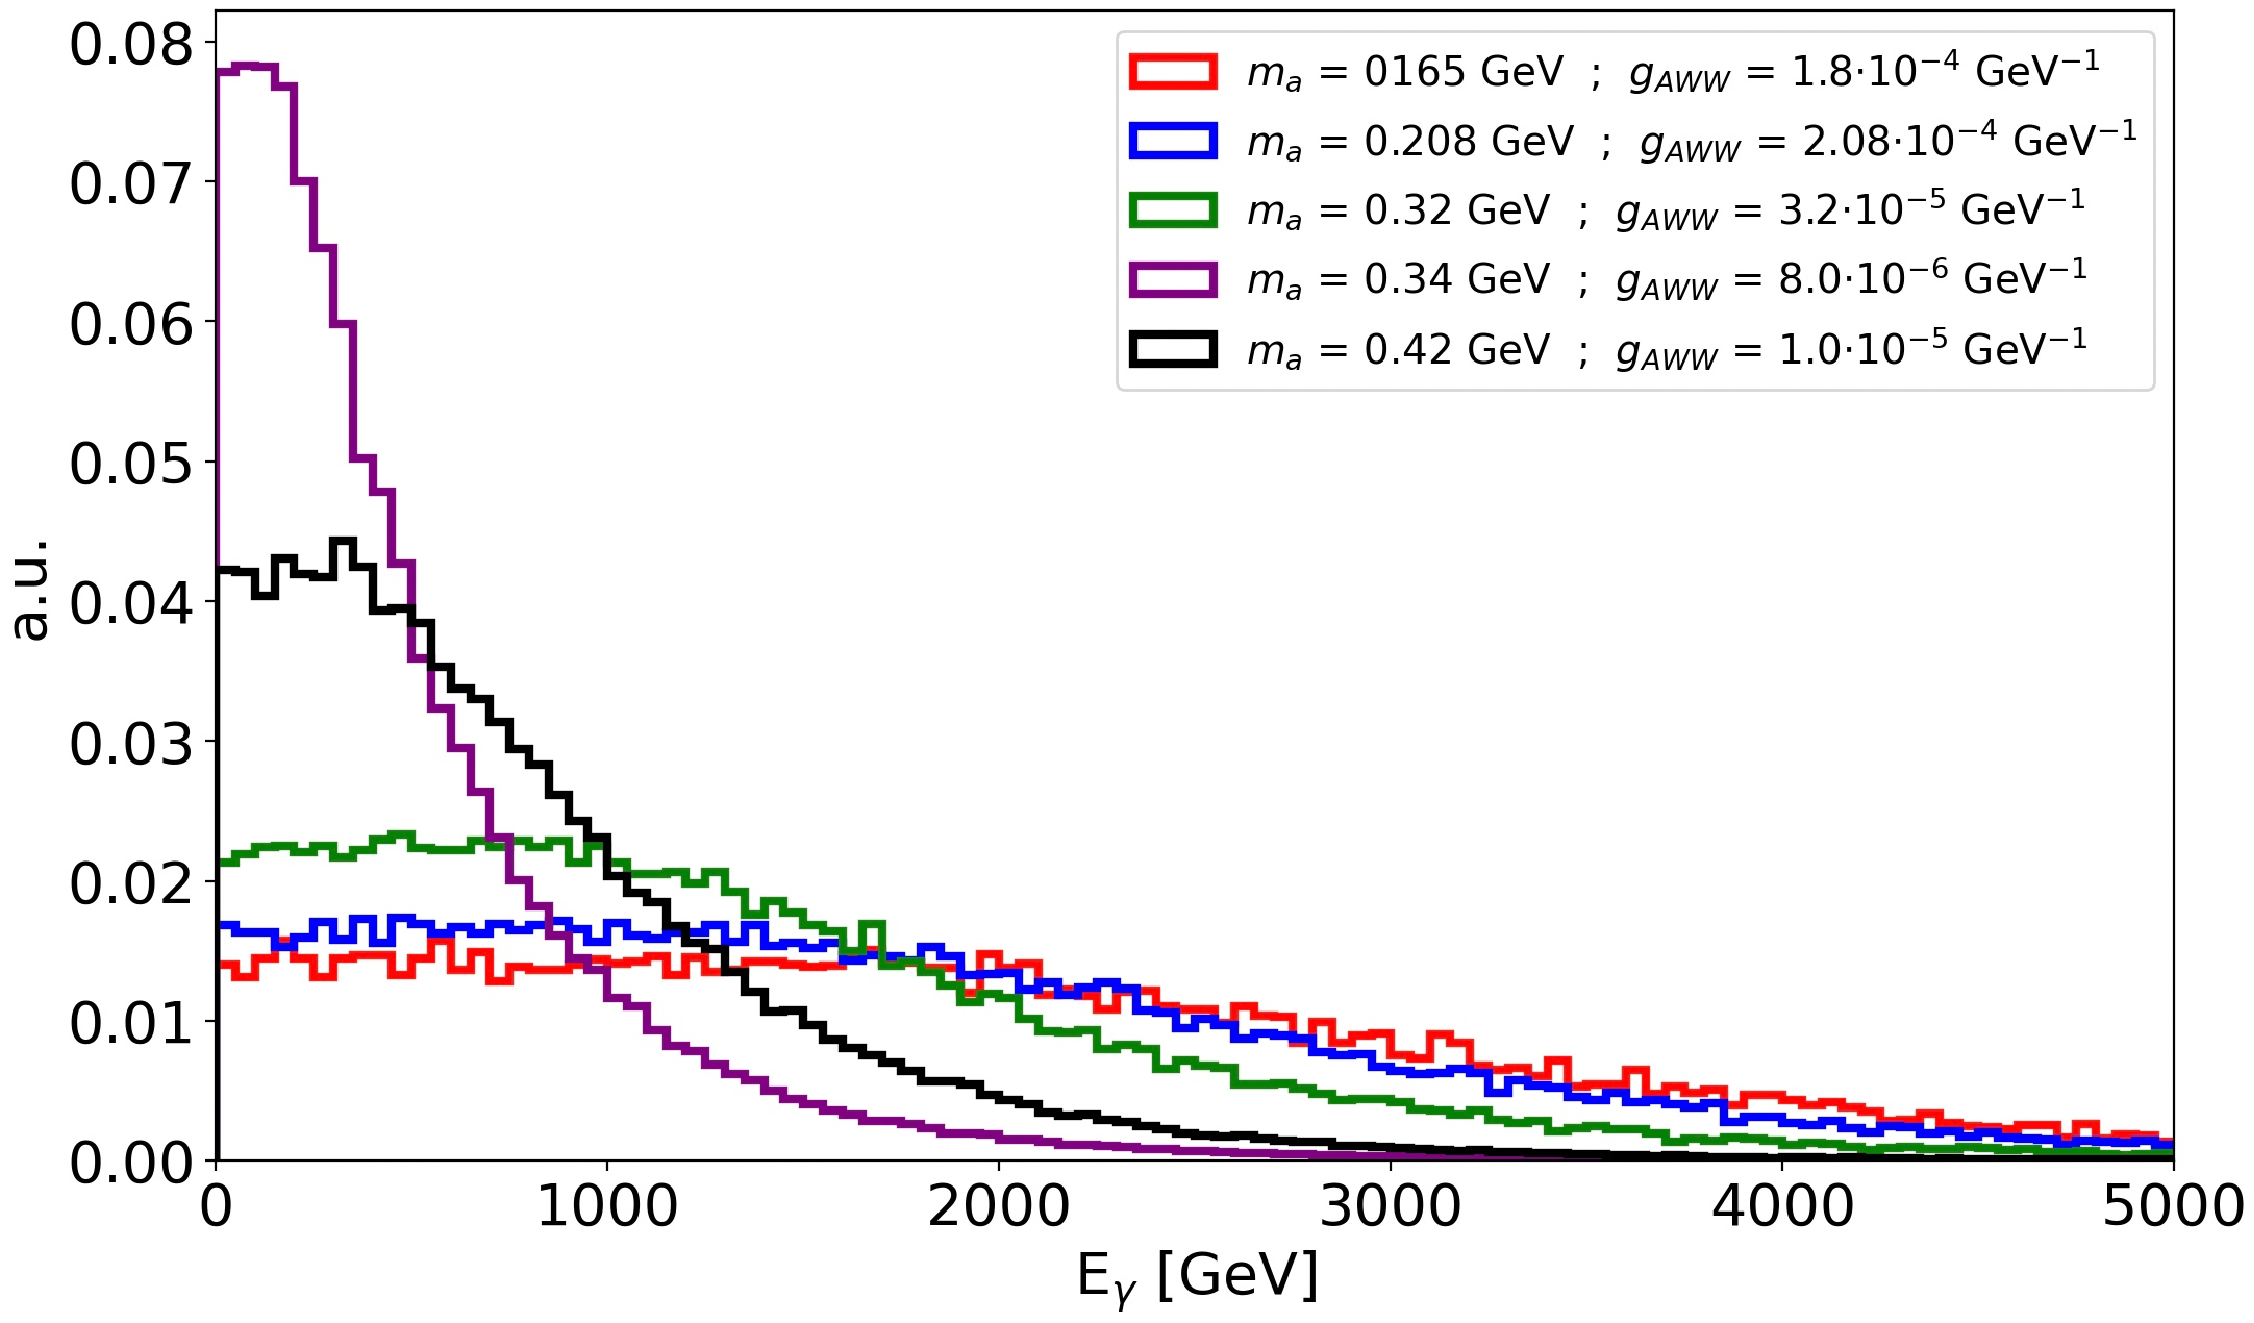
\includegraphics[width=0.8\linewidth]{files/ALP_photon_energy}
			\caption{Energy distribution of the photon emerging from ALP decays for different combination of ALP mass $m_a$ and coupling $g_{aWW}$.}
			\label{im:ALP_photon_energy}
		\end{figure}
		
		It is also interesting to better under the topology of the di-photon production to look at the distribution of number of events in the plane defined by the energy of the two photons separately. This was performed in the studies carried out in \cite{Moretti_MasterThesis} and the results is presented in figure \ref{im:ALP_E1E2_distribution}.
		\begin{figure}[h]
			\centering
			
\includegraphics[width=1.0\linewidth]{files/ALP_E1E2_energy}
			\caption{Energy distribution of the photon emerging from ALP decays for different combination of ALP mass $m_a$ and coupling $g_{aWW}$. The number of events in the top right corner of every figure is given for an integrated luminosity of 90 fb$^{-1}$.}
			\label{im:ALP_E1E2_distribution}
		\end{figure}
		
		As expected the energies of the photon are fully correlated. The distribution show that their exist both events with very similar energies for the photon than events in which the two energies are considerably different. The energies of the two photons depends on the decay angle in the center of mass frame of the ALP, once boosted one of the photon can be very soft while the second one carries most of the momentum of the ALP. To complete the study of ALP production rate, a sensitivity reach plot given in figure \ref{im:reach_plot_ideal} was produced in the mass and coupling. As in the sensitivity reach presented in figure \ref{im:ALP_photon_prod}, an ideal detector with full efficiency and no background events was assumed. Two different reach are presented for different integrated luminosity corresponding to LHC Run3 and HL-LHC.
% TODO CH2: change the scale of the axis and title to match the ones that are bigger in the plots below. 
		\begin{figure}[h]
			\centering
			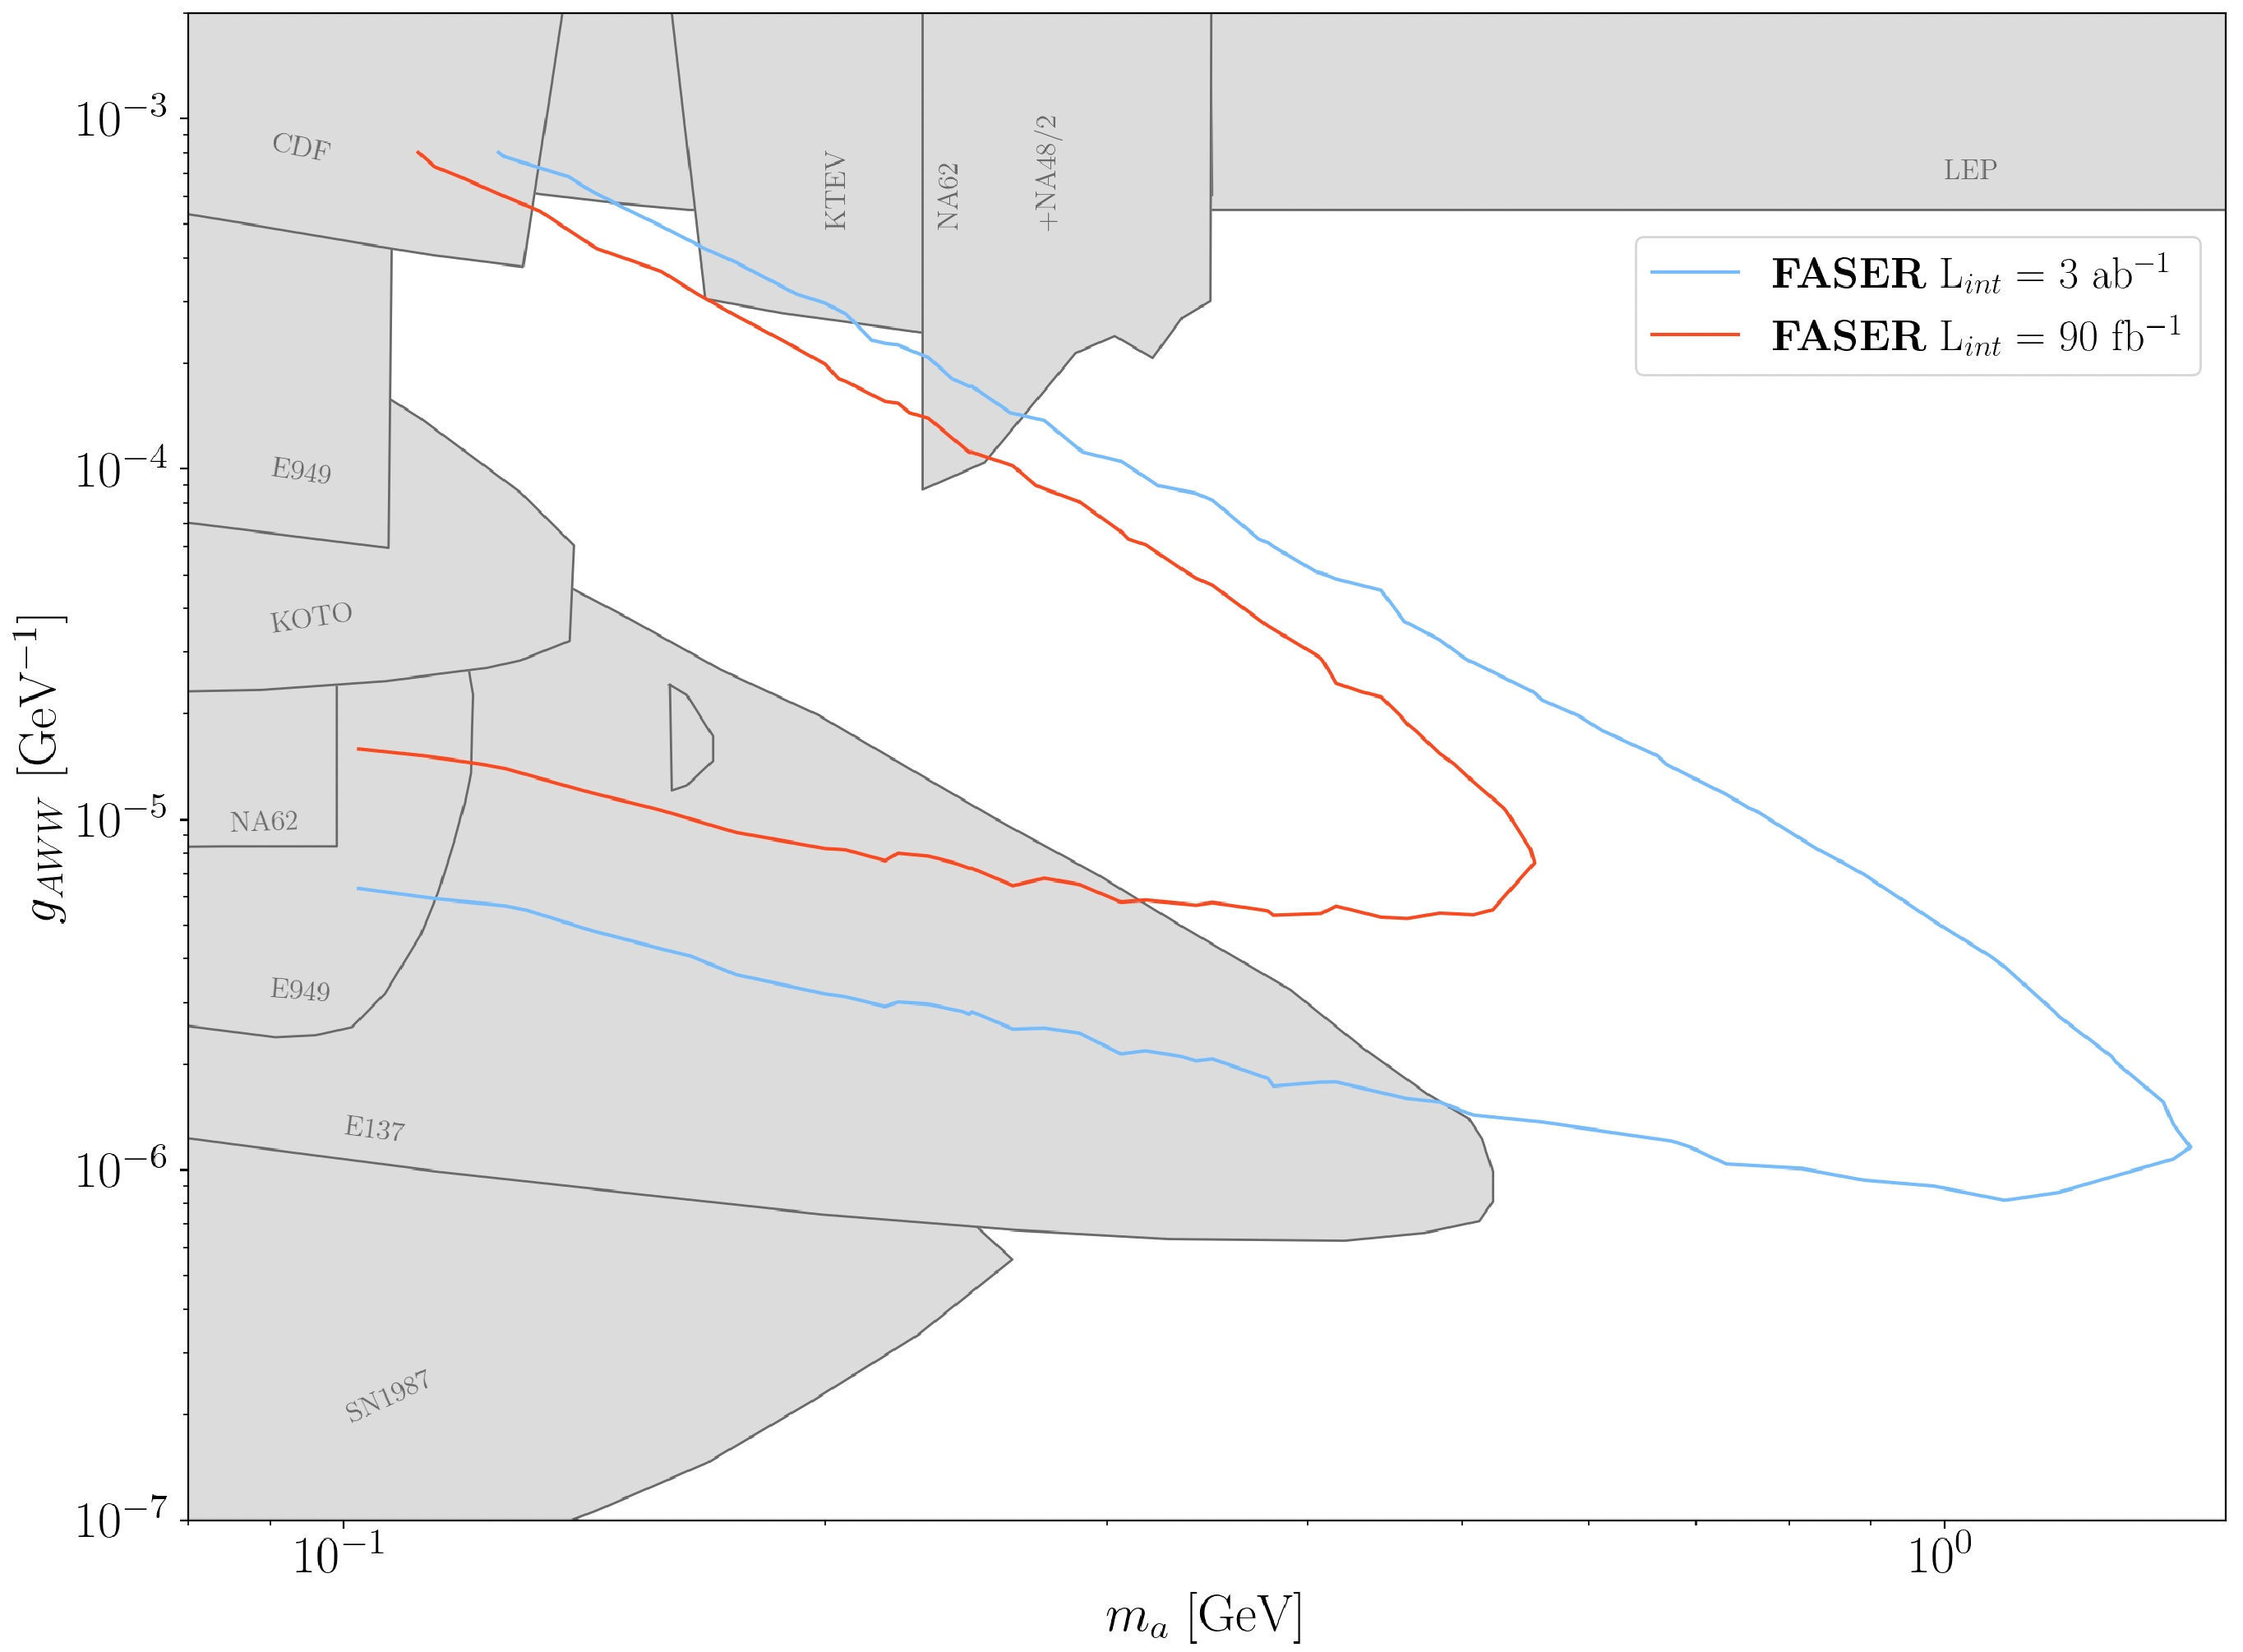
\includegraphics[width=0.8\linewidth]{files/reach_plot_ideal}
			\caption{Sensitivity reach plot for ALP decay into a photo pair wit the FASER detector assuming full detection efficiency. The areas in grey correspond to region in the parameter space already constrained by other experiments. The reach is given for an integrated luminosity of 90 fb$^{-1}$ for the LHC Run 3 (in red) and for 3000 fb$^{-1}$ for the HL-LHC.}
			\label{im:reach_plot_ideal}
		\end{figure}
		
		As one could easily guess, there exists no detection system, even as elegant as one could imagine, that is able to produce a detection efficiency of 100 $\%$. For the sake of having a more truthful description of the discoveries prospects, a detector layout with its main characteristics needs to be specific. This will be the argument addressed in the ensuing discussion. 
		
		\subsection{Sensitivity reach with new PreShower detector}
		
		The detection of the two photons produced in ALPs decay can be performed through the detection of the electromagnetic shower produced by photon converting in an absorber material. Since the produced ALPs are very boosted, the photons will be emitted very close-by and a detector with fine granularity in the transverse plane is required. In order to have redundancy and avoid identifying as photon showers fake events or statistical fluctuation in the shower development, having a sampling over various detector planes of the shower profile can be an advantage. 
		
		In 2020 at the University of Geneva (UniGe), the idea of replacing the original pre-shower station with a fine granularity pre-shower saw light for the first time. In parallel to the studies of ALP production in a novel channel, a first design of the new pre-shower was first drown. The pre-shower's layout remained quite simple and was made of six identical planes composed of roughly 1.3 $X_0$ on tungsten for the absorber part and a plane of monolithic silicon pixel detector for detecting the photon electrons and positrons generated in the electromagnetic shower from the converted photons. It is then interesting to see how the typical decay signatures in FASER would be with the upgraded layout. The signatures are presented in figure \ref{im:FASER_DP_signature_newPS} and figure \ref{im:FASER_ALP_signature_newPS}. 
		
		\begin{figure}[h]
			\centering
			\includegraphics[width=1.0\linewidth]{files/FASER_DP_signature_newPS}
			\caption{Dark photon typical decay signature with new pre-shower station.}
			\label{im:FASER_DP_signature_newPS}
		\end{figure}
		
		\begin{figure}[h]
			\centering
			\includegraphics[width=1.0\linewidth]{files/FASER_ALP_signature_newPS}
			\caption{ALP typical decay signature with new pre-shower station.}
			\label{im:FASER_ALP_signature_newPS}
		\end{figure}
		
		The new typical signatures for the dark photon and ALP decay are to be compared with figure \ref{im:FASER_OLD_DP_signature} and figure \ref{im:FASER_OLD_ALP_signature} respectively. For the dark photon studies, the additional position measurement brought by the six pixel detector planes could help improve the quality of the signal in the case of very close-by tracks. For the ALP, it is possible to distinguish between events with one or more photons as the preshower makes photons converts in the tungsten and the 6 detectors planes are sampling the development of the electromagnetic shower. 
 		  
		In the detector specifications proposed at the time of the studies, the pixel pitch was considered to be \SI{100}{\micro\meter}, meaning that the photons would need to be separated by at least \SI{200}{\micro\meter} to be distinguishable. Simulations of the detector performance with GEANT4 were performed. ALP decay events were produced for two photons whose energies could take any value in $E_\gamma$ = [250, 350, 450, 750, 1000, 1500, 2000, 3500] GeV and for a separations between the photons with values in $\delta_{\gamma\gamma}$ = [0.2, 0.3, 0.5, 1.0, 2.0] mm. An event display of the showers from two photons in the sixth detector plane with energies $E_{\gamma,1} =$ \SI{750}{\giga\electronvolt} and $E_{\gamma,2} =$ \SI{1.5}{\giga\electronvolt} with separation of $\delta_{\gamma\gamma}$ = \SI{200}{\micro\meter} is presented in figure \ref{im:di-photon_event_GEANT4} and was taken from \cite{PreShower_TP}. 
		
		\begin{figure}[h]
			\centering
			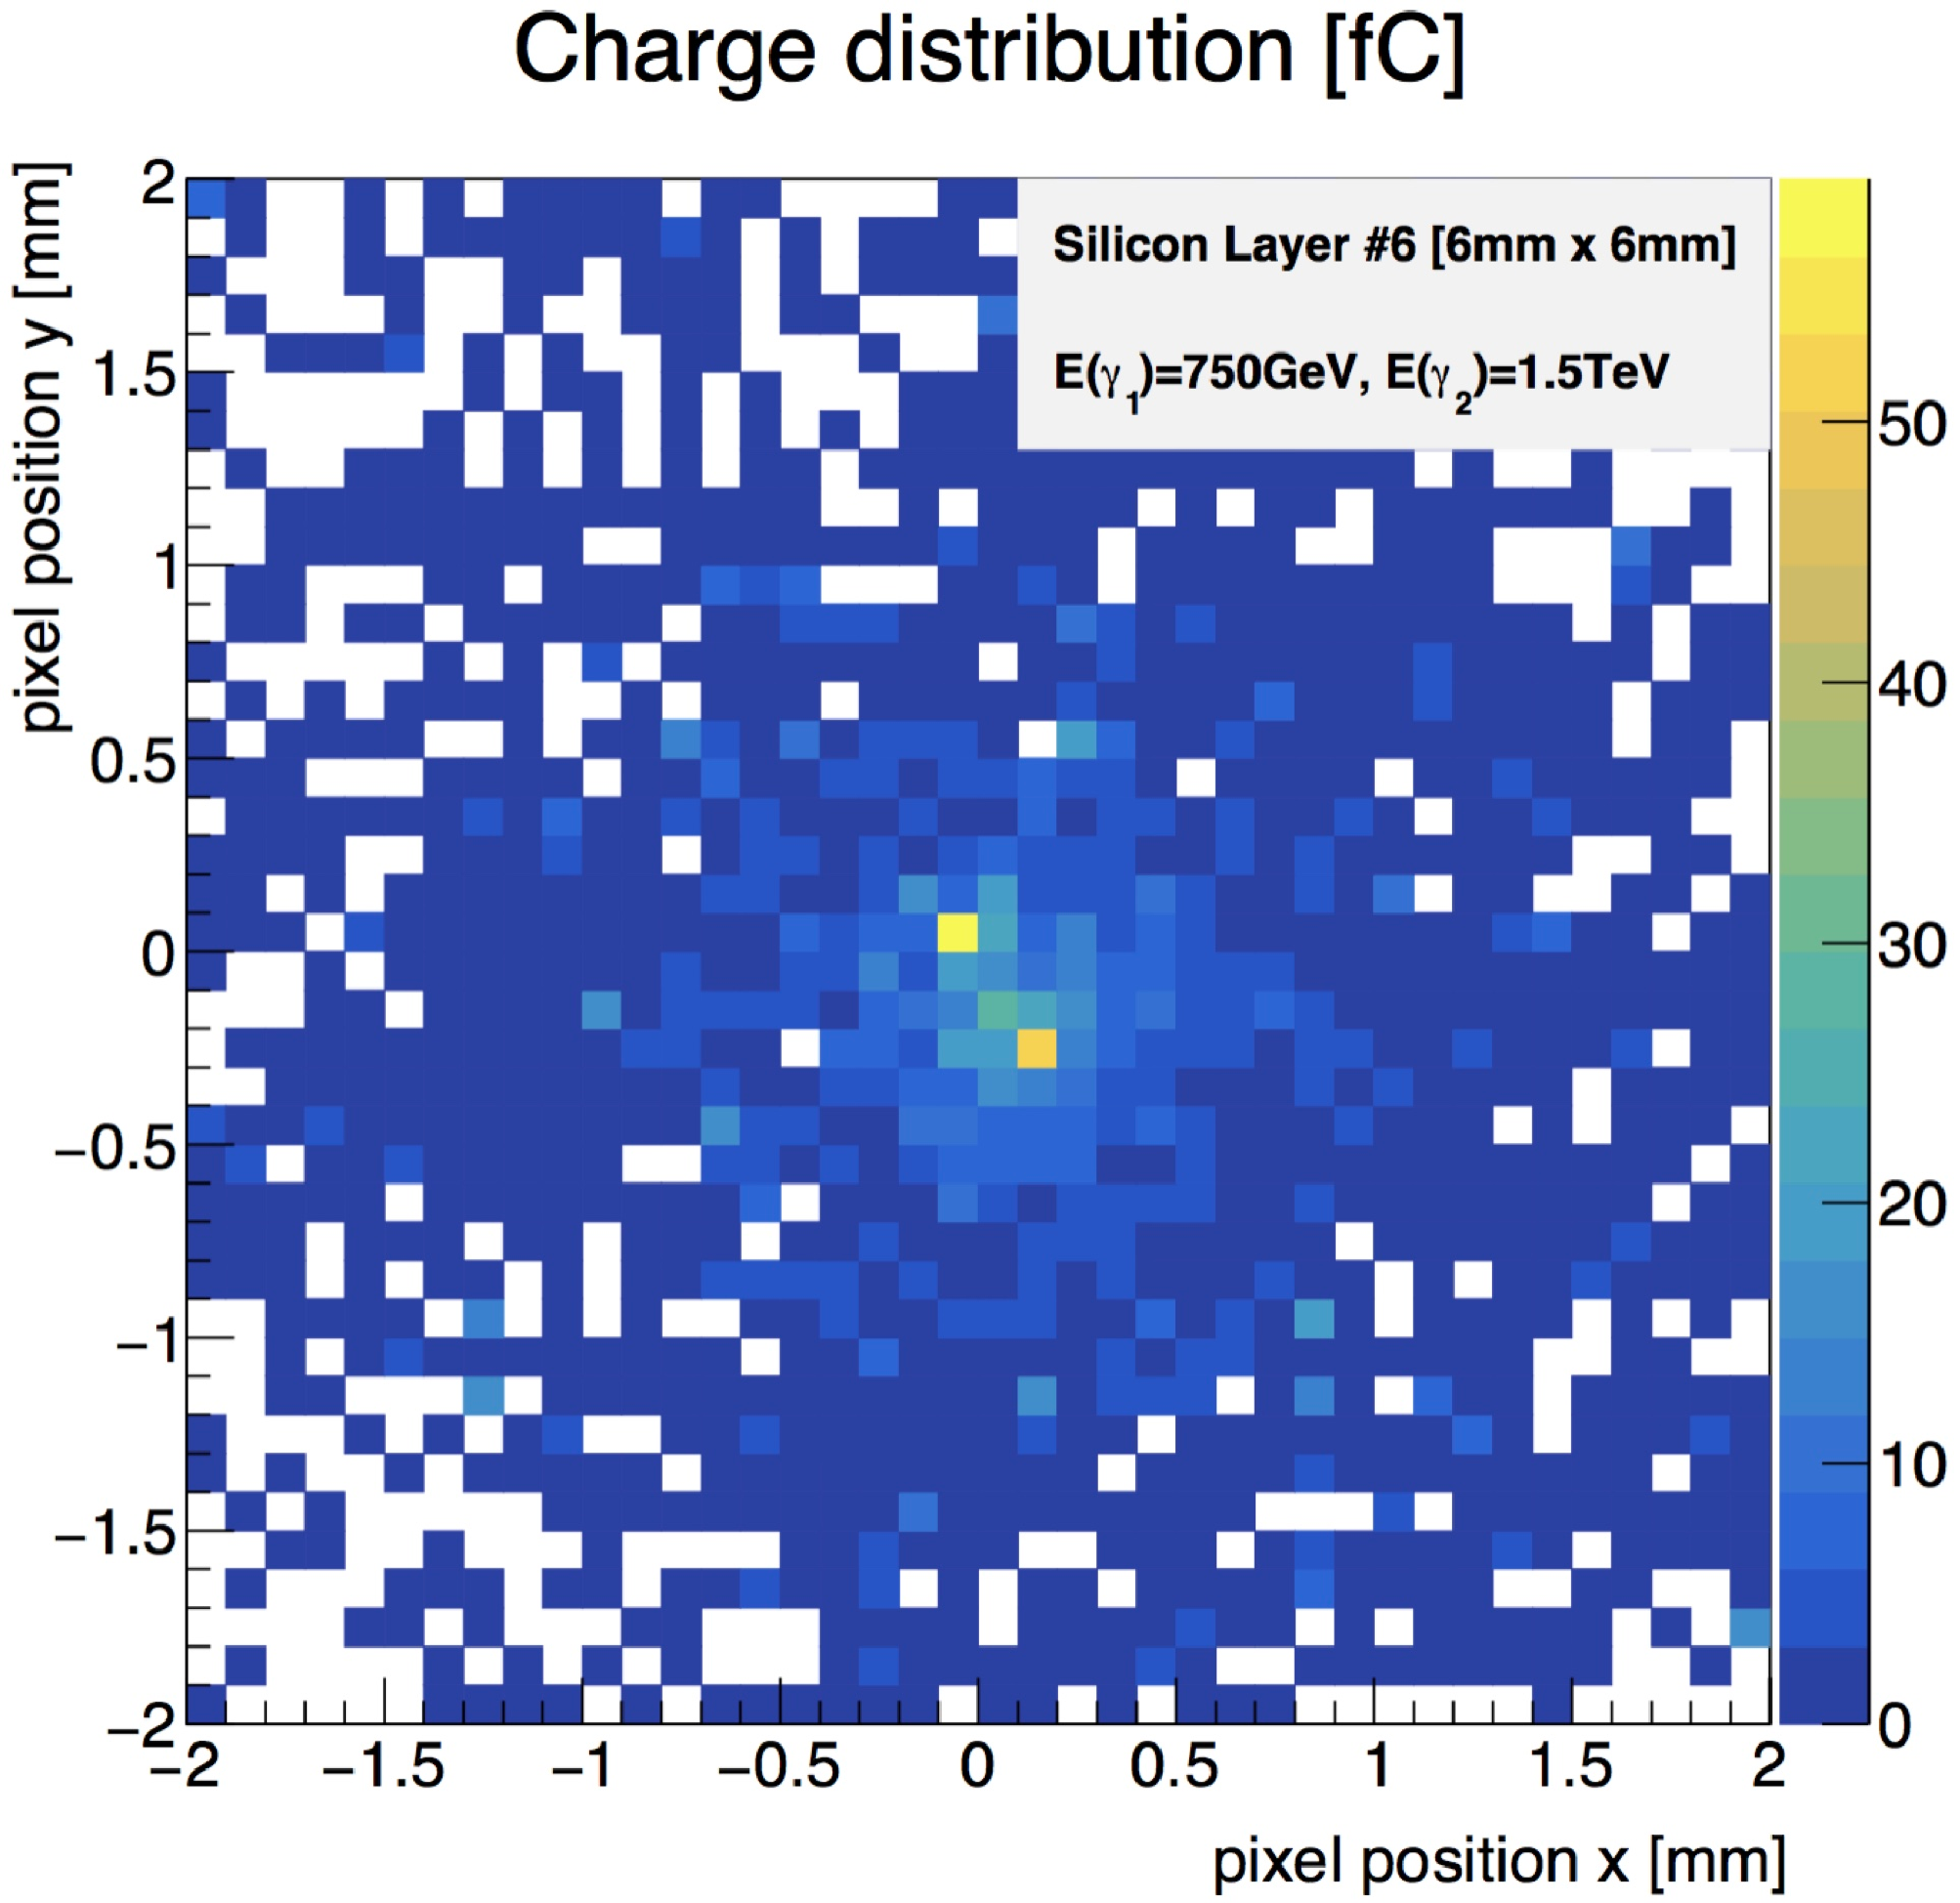
\includegraphics[width=0.7\linewidth]{files/di-photon_event_GEANT4}
			\caption{Event display for the decay of an ALP in two photons with $E_{\gamma,1} =$ \SI{750}{\giga\electronvolt} and $E_{\gamma,2} =$ \SI{1.5}{\giga\electronvolt} and separation $\delta_{\gamma\gamma}$ = \SI{200}{\micro\meter}. The charge deposited by the electromagnetic showers from the two photons is given in fC by the colour scale.}
			\label{im:di-photon_event_GEANT4}
		\end{figure}
		
		The electromagnetic showers from each photon are mixing and are characterised by a low charge deposition across a large region with a much higher charge deposition at the center of the shower fo each individual photon. The position of the photon can be reconstructed as the center of shower where the amount of deposited charge is the highest. A simple photon-reconstruction algorithm was developed to reconstruct the position of the photons using the charge deposition in each pixel across the different detector planes \cite{PreShower_TP}. The detection efficiency was estimated for all of the possible combinations of photon energies and separations cited previously.  
		
		The minimal separation between the photons to be distinguished will have an effect on the number of ALP signals FASER will be able to identify as so. Taking the discussion back into the MC simulations for the ALP, once can see what the effect of the minimal photon separation would be on the distributions previously presented in figure \ref{im:ALP_E1E2_distribution}. The results are presented in figure \ref{im:ALP_E1E2_distribution_cut} and were taken from \cite{Moretti_MasterThesis}. 
		 
		\begin{figure}[h]
			\centering
			
\includegraphics[width=1.0\linewidth]{files/ALP_E1E2_energy_cut}
			\caption{Energy distribution of the photon emerging from ALP decays for different combination of ALP mass $m_a$ and coupling $g_{aWW}$. A selection of events was performed with the criteria that the separation between the two photons when reaching the preshower is greater than $\delta_{\gamma\gamma}$ = \SI{200}{\micro\meter}. The number of events in the top right corner of every figure is given for an integrated luminosity of 90 fb$^{-1}$. The top number is the number of events after the selection criteria while the bottom number is the total number of events.}
			\label{im:ALP_E1E2_distribution_cut}
		\end{figure}
		
		It is striking to observe that a large part of the number of events can disappear, as for example for the benchmark model with mass and coupling values $\left[0.165, 1.8\cdot 10^{-4}\right]$, when comparing figure \ref{im:ALP_E1E2_distribution} and figure \ref{im:ALP_E1E2_distribution_cut}, one can see that the region with photon energy very similar to one another disappeared, leading to a decrease of the number of events of more than 50$\%$. It is also interesting to note that the effect is less important for ALP with lower average energies (as for example the benchmark model with values $\left[0.32, 3.2\cdot 10^{-5}\right]$). Indeed the higher the momentum of the ALP, the more important the Lorentz boost when computing the angles of emission of the photons in the laboratory reference frame and the closer the photons. \\
		
		In order to adapt the sensitivity reach presented in figure \ref{im:reach_plot_ideal} for a more realistic detector, one would need to add the reach as a function of the minimum separation between the photons as it has a drastic effect on the number of events. The number of events was then estimated as a function of the energy of the two photons and their separation for every ALP model with mass $m_a$ and coupling $g_{aWW}$. The number of events where the scaled to the detection efficiencies obtained with the GEANT4 MC simulations and the obtained results from \cite{Moretti_MasterThesis} are shown in figure \ref{im:reach_plot_detector}.
		\begin{figure}[h]
			\centering
			
\includegraphics[width=1.0\linewidth]{files/reach_plot_detector}
			\caption{Sensitivity reach of the new FASER pre-shower detector for different separations between photons. The results are presented for an integrated luminosity of 90 fb$^{-1}$ (left) and 3000 fb$^{-1}$ (right).}
			\label{im:reach_plot_detector}
		\end{figure}
		The results show that the reach for a fixed integrated luminosity changes a a function of the criteria on the minimum separation between the two photons. As expected, the larger the separation criteria and the lower the number of events, this leads to the reach shrinking for higher separations values. Nonetheless, even with a minimal separation of \SI{200}{\micro\meter}, the deviation from the ideal reach is not significant and a large portion of the yet unconstrained parameter space could be probed by FASER. 
		
		In addition to the enhanced sensitivity to ALP di-photon signals, the new design of the pre-shower station will also contribute to the dark photon searches or any model with similar final state ( pair of oppositely charged leptons). The pre-shower allows for more measurements of charged particles at the back of the detector and with a better spatial resolution than the original detector. The addition of this position measurement could allow to separate very closely spaced tracks which can't be separated with the current detector and could even allow for an increase of the length of the decay volume to include the second magnet, increasing the acceptance by 70$\%$ \cite{PreShower_TP}. The pre-shower will also make the overall detector more robust to inefficiencies in the back tracing station. 
		The drawback fo the new pre-shower design is the amount of material present in front of the calorimeter. A degradation in the energy resolution of the calorimeter station could be expected but a correction using the charge measured in the different pre-shower detector planes could help. Nevertheless, it is not expected that the degradation of the energy resolution will have a significant impact on the physics of FASER \cite{PreShower_TP}.\\
		
		The discussion on the FASER detector and its physics program is now over. A few of the leading BSM models in the sensitivity reach of FASER were discussed together with the prospects in reaching higher sensitivity for any model predicting a photonic final state such as the ALP model discussed. The introduction of a "monolithic silicon pixel detector" for the active parts of the new pre-shower station was actually a good hint to the argument discussed in the next chapter. 
		


		
		
		
		
		
		
		
		
		
		
		
		
		
		
		
		
		
		
\clearpage

\chapter{Monolithic silicon pixel detectors}\label{ch:2}

The first particle detection experiments at accelerator were usually set-up following the fixed target approach meaning that the beam of incoming particles would be shot on a stationary target. The detector for these particular experiments would then cover a rather small region in space and in momentum to detect single particles produced in the interaction. Simply scanning as the function of angle and momentum acceptances, the number of particles with a counter, one could reconstruct the kinematics of the particles. Concurrently, since the 1950s, other detector layouts like bubble chambers allowed physicist to register at a larger scale the full interaction of the particles involved, but the analysis work of the single exposures turns the detecting method very laborious. 

For quite some time, optical recording by photographic exposures remained the only choice to capture complex particle interaction within large detecting volumes. Although, since the 1960s, the transition towards detectors profiting from fully electronic readout started in parallel to the development of highly integrated circuits. This advancement in technology brought a solution to the arduous readout of bubble chambers but in environments such as the LHC were high radiation levels are encountered, the rates limitations from technologies such as MultiWire Proportional Chambers (MWPCs) forced by the large collections electrodes slowly became a problem too. 

In modern particle physics, the fixed target approach is often disfavoured to the head on or collider type of experiments in which bunches of particles are both accelerated and collide at the core of a detector. The goal is then to cover as much as possible of solid angle around the interaction point, detecting, identifying and kinematically reconstructing all the particles produced in the scattering process. If one had to give a general description of the detectors designed for collider experiments, it would generally be constructed in a cylindrical arrangement around the accelerator's beam pipe. It would notably require in its inner parts a vertex detector and tracking detectors respectively for identification of secondary vertices from the initial reaction vertex and reconstruction of tracks leading to momentum reconstruction and in some cases also particle identification\ \cite{detectors}. 

The high event rates combined with high spatial resolution required and low amount of material needed in the innermost layers of the detectors put in evidence semiconductors detectors as the preferred solution for the future experiments. This direction was even more praised by the fast development of microelectronics technics and their intrinsic properties such as densities and low energy threshold required for ionisation. Recent studies in this field has also proven this technology to be providing excellent timing performances which, as discussed previously, will be one of the key requirement for future particle tracking systems at collider experiments. In the following chapter a description of semiconductors devices for particle detection will be provided, and some more advanced concepts will be discussed as part of the focus of this work. 

	\section{Fundamentals of semiconductors}\label{sec:2.1}
	Semiconductors are classified together with insulators and conductors as one of the three type of solid material. Their electric resistivity (or equivalently electrical conductivity) is found in between the range of insulators ($10^8$ \SI{}{\ohm\centi\meter} and above) and the one of conductors ($10^-3$ \SI{}{\ohm\centi\meter} and below). Different types of pure semiconductors or compound will have different resistivities. Silicon (Si) is the most widely used semiconductor both for the detection material and readout chip of the present detectors, thanks to its large abundance on Earth but also to its intrinsic properties which will be discussed later.

		\subsection{Intrinsic and doped semiconductors}\label{subsec:2.1.1}
		The different properties of semiconductors are defined by the arrangement of the atoms within their crystalline structure. Silicon crystals are arranged in a diamond lattice so that each Si atom is covalently bonded to four nearest neighbors arranged at the corners of a tetrahedron\ \cite{SolidState}. From this specific structure, the diverse crystal planes are usually used for slicing the crystals to obtain a different arrangement and density of atoms and hence different properties for various applications using the same semiconductor material\ \cite{Si_Crystals_planes}. 

		The compact and periodic arrangement of atoms in the lattice give rise to a separation so thin in the energy levels of individual atoms due to the influence of many neighbouring atoms that one has to consider energy bands rather than single energy levels. The energy bands are separated by a so-called band-gap and the electrical conduction properties are defined by the two highest energy bands respectively the valence band and the conduction band. The conduction properties really depend on the energy difference between the bands as the energy levels within the bands themselves are so dense that transitions to unoccupied levels can seamlessly be done.
		\begin{figure*}[h]
		\begin{minipage}{0.49\linewidth}
		For insulators, the valence band is completely filled due to the very strong bonds between the neighbouring atoms, the conduction band is then empty, and the band gap is very large, about \SI{9}{\electronvolt} at room temperature. It is then very unlikely that by thermal excitation, an electron can rise from the valence band to the conduction band, current can't flow in insulators. In semiconductors, the neighbouring atoms are less bonded to each other, this leads to a smaller band gap energy, for Silicon it is about \SI{1.12}{\electronvolt} at room temperature. By thermal excitation of the action on an electric field, an electron can be moved to the conduction band leaving behind a hole in the valence band, current can then flow. 

		\end{minipage}\hfill
		\begin{minipage}{0.49\linewidth}
		\centering
		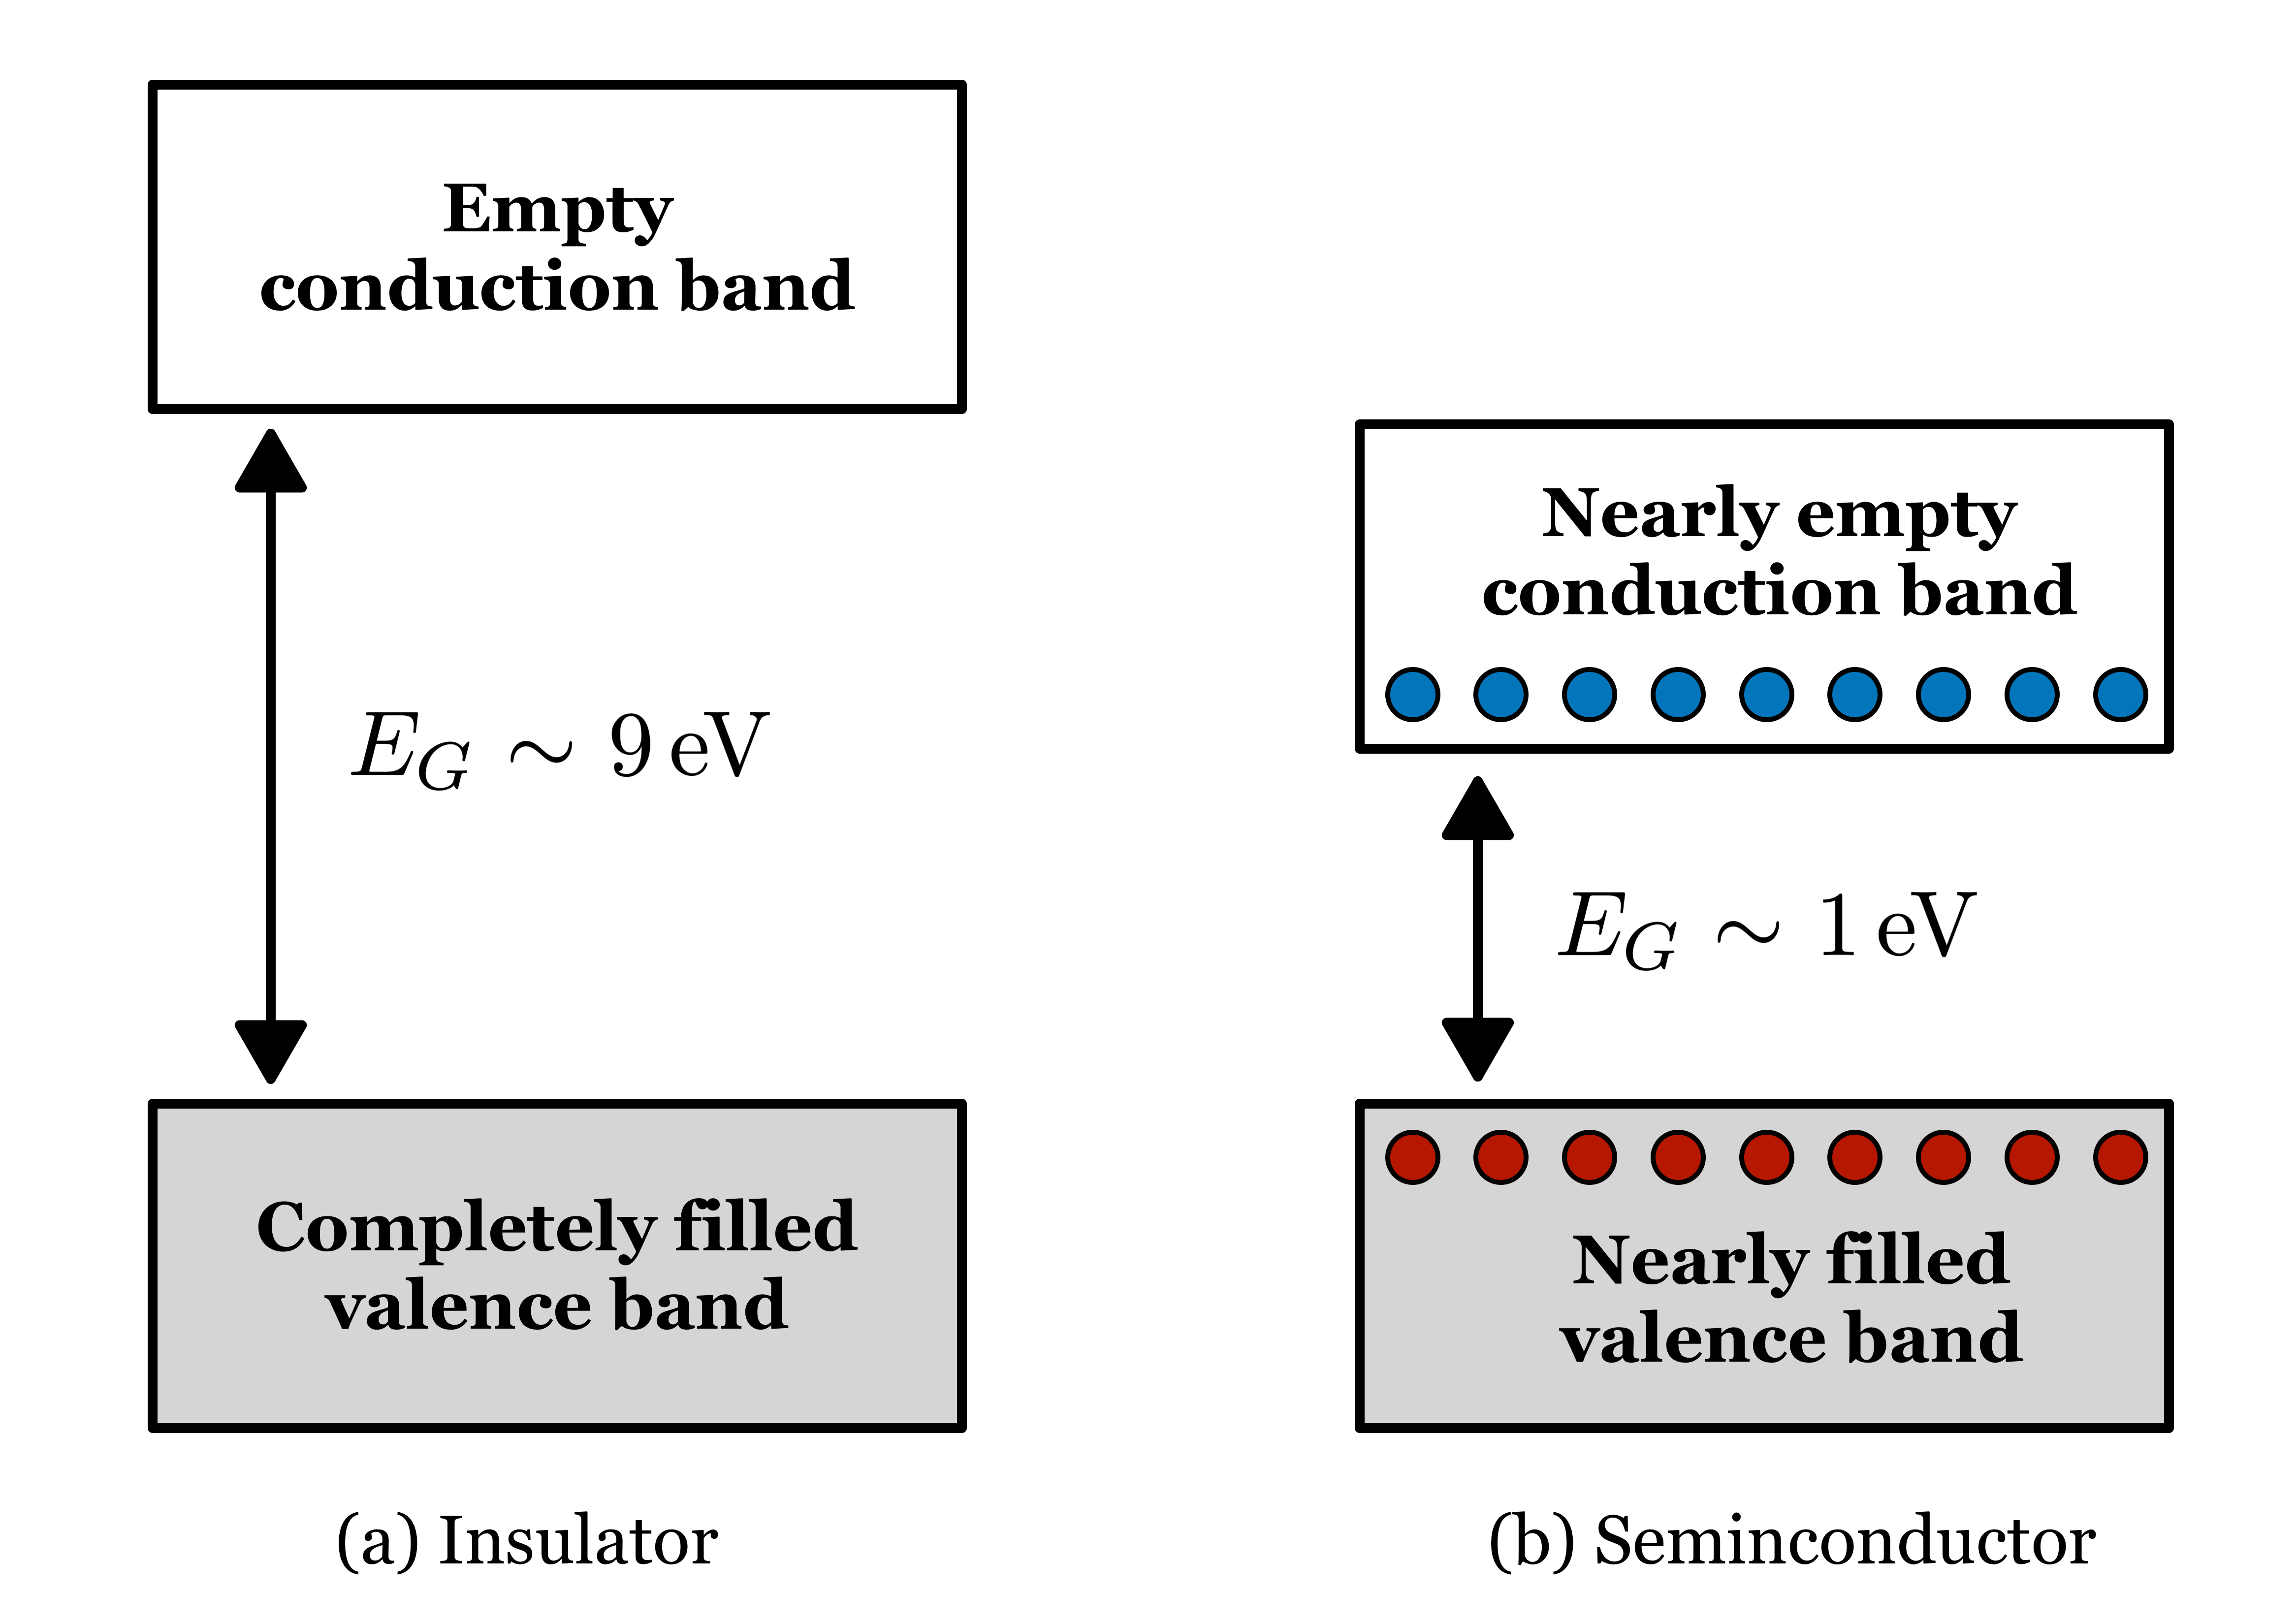
\includegraphics[width=1.0\linewidth]{files/energybands_insu_semi}
		\caption{Schematic view of the separation between valence and conduction bands for a) an insulator and b) a semiconductor.}
		\label{ }
		\end{minipage}
		\end{figure*}

		The gap in energy separating the bands can be influenced by temperature or pressure as it is directly linked to the spacing inside the crystal's lattice. Indeed, for Silicon it goes from \SI{1.17}{\electronvolt} at \SI{0}{\kelvin} down to \SI{0.92}{\electronvolt} at \SI{800}{\kelvin}\ \cite{PhysicsOfSemiconductors}. At the lowest temperatures most of the electrons are in the valence band and do not contribute to the conduction, at absolute zero temperature, all the electrons are in the valence band. The aforementioned holes left in the valence band also contribute to the conduction if one interprets them as positive charge carriers as opposed to electrons. 

		Inside a crystal, the periodicity of the lattice potential gives rises to the definition of effective mass for the electrons and the holes. Indeed, the wave vector $\vec{k}$ of an electron or hole is not proportional to the eigenstate of the solution to Schrödinger's equation but rather depends on a generalised lattice momentum $\hbar \vec{k}$ such that the energy of the electrons or holes depends on this later such that $E = E(\vec{k})$. One can then define the effective mass as follows: 
		\begin{equation}
			\frac{1}{m_{ij}^*} = \frac{1}{\hbar^2}\frac{\partial^2 E(k)}{\partial k_i \partial k_j}
			\label{eq:effective_mass}
		\end{equation}

		We can see the dependence here on the band curvature in momentum space but also on the direction of movement of the electron or hole in the crystal lattice.
		
		\subsubsection{Intrinsic semiconductors}

		In order to give a comprehensive description of the electrical properties of semiconductors, it is important to discuss the charge carrier concentration in thermal equilibrium, first for intrinsic semiconductor and then understand how this one change once introducing external impurities (doping) inside the crystal. To define the charge carrier concentration $n(E)$, one needs to consider the number of states that electrons and holes can occupy per unit volume and energy, called density of states $Z(E)$ and their occupation probability $f(E)$, such that: 
		\begin{equation}
			n(E) dE = Z(E) f(E) dE
		\end{equation}

		In momentum space, in the shell between two spheres of radii $p$ and $p + dp$, one finds a volume $4\pi p^2 dp$, and knowing that states occupy each a volume $h^3$ in momentum space, one can write: 
		\begin{equation}
			Z(p) dp = \frac{2}{h^3} 4 \pi p^2dp
		\end{equation}
		The factor $2$ comes from the nature of the charge carriers, being fermions, more than one electron or hole can occupy the same energy state if their spin have opposite projections. As we want an expression od the density of states as a function of the energy, one can use the non-relativistic dispersion relation to obtain: 
		\begin{equation}
			\begin{split}
				\frac{dE}{dp} = \frac{p}{m^*} &\Rightarrow dp = \frac{m^*}{p} dE = \frac{m^*}{\sqrt{2m^*E}}dE\\
																			&\Rightarrow 4\pi p^2 dp = 8 \pi \frac{(m^*)^2}{\sqrt{2m^*E}}EdE\\
																			&\Rightarrow Z(E)dE = 4 \pi{ \left( \frac{2m^*}{h^2} \right)}^{3/2} \sqrt{E} dE
			\end{split}
		\end{equation}

		We have found that the density of states $Z(E)$ per volume and energy, increases proportionally to the square root of the energy of the states occupied by the electron or hole. 

		Moving to the occupation probability of the states $f(E)$, the spin-$1/2$ nature of both charge carriers suggest a distribution within the energy band of the quantum energy states following the Fermi-Dirac distribution such that: 
		\begin{equation}
			f_n(E) = \frac{1}{\exp(\frac{E-E_f}{kT}) + 1} \hspace{5mm} \text{and} \hspace{5mm} f_p(E) = \frac{1}{\exp(\frac{E_f-E}{kT}) + 1}
			\label{eq:FermiDirac}
		\end{equation}

		We have used in the above equation $k$, the Boltzmann constant, $T$ the temperature and $E_f$ the Fermi energy, defined as the energy for which, at $T=\SI{0}{K}$ none of the states with energy $E > E_f $ are occupied and at $T > \SI{0}{K}$, the energy having an occupation probability of 50$\%$. The expression on the left, $f_n(E)$ as subscript $n$ for negative charge carries, the electrons, whilst the expression on the right, $f_p(E)$ as subscript $p$ for positive charge carries, the holes. 
		\begin{figure}[h]
		\centering
		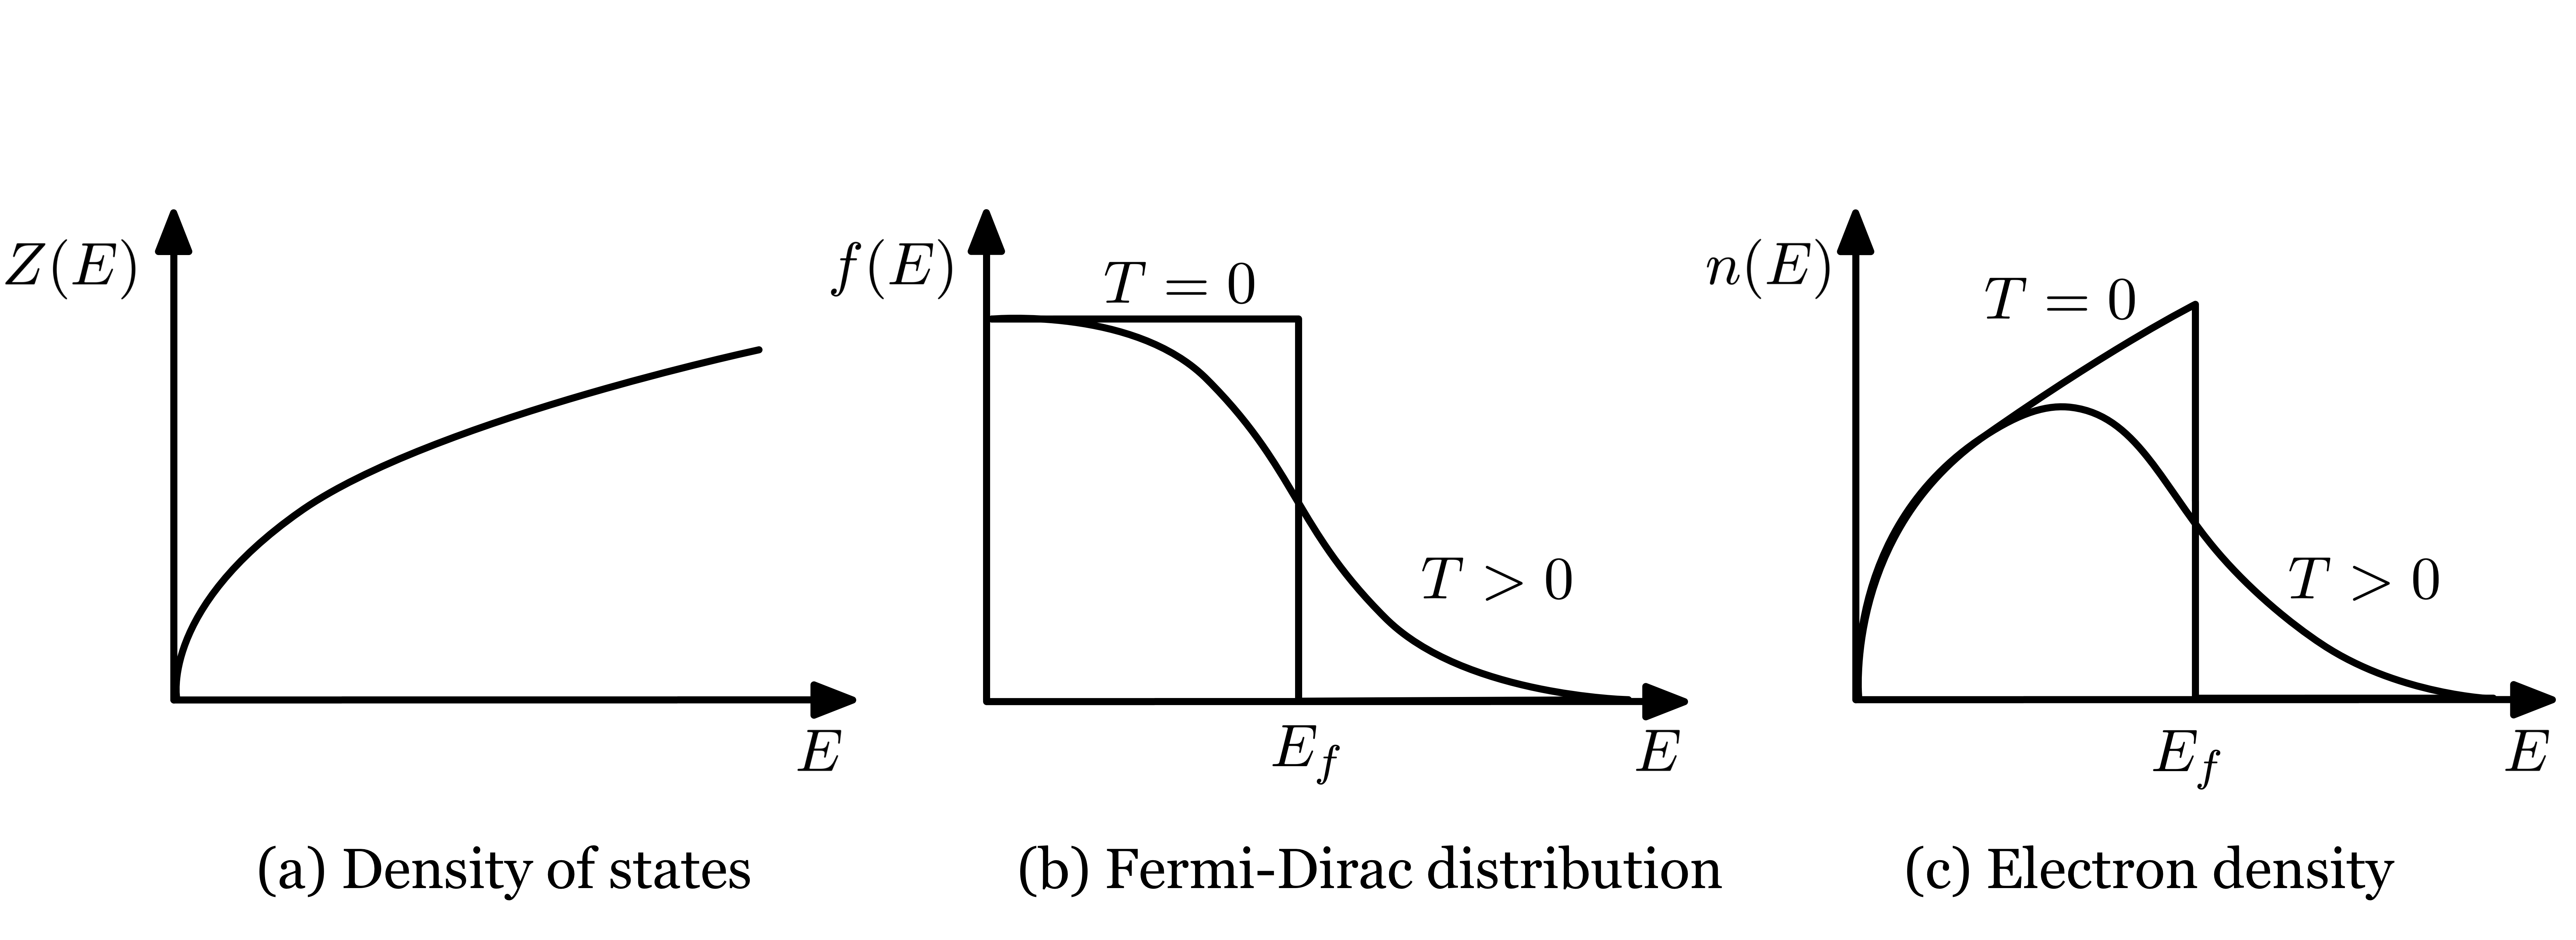
\includegraphics[width=0.9\linewidth]{files/density-fermidirac}
		\caption{Density of states a), Fermi-Dirac distribution b) and electron density c)}
		% \label{ }
		\end{figure}

		It is then fundamental to take into consideration, for semiconductors, the effect of band of available energy level and especially the band gap separating the conduction and valence band as follows: 
		\begin{equation}
			Z_n(E)dE = 4 \pi {\left(\frac{2m_n^*}{h^2}\right)}^{{3/2}} \sqrt{E-E_{C}}\ \Theta(E-E_C)dE
		\end{equation}
		\begin{equation}
			Z_p(E)dE = 4 \pi {\left(\frac{2m_p^*}{h^2}\right)}^{{3/2}} \sqrt{E_V-E}\ \Theta(E_V-E)dE
		\end{equation}

		The Heaviside function $\Theta$ accounts from the sudden transition at the band's edges to the gap. One can thus multiply the respective density of states for positive and negative charge carriers to the energy states distributions discussed in \eqref{eq:FermiDirac} to obtain the charge carrier concentration. 

		\begin{figure}[h]
			\centering
			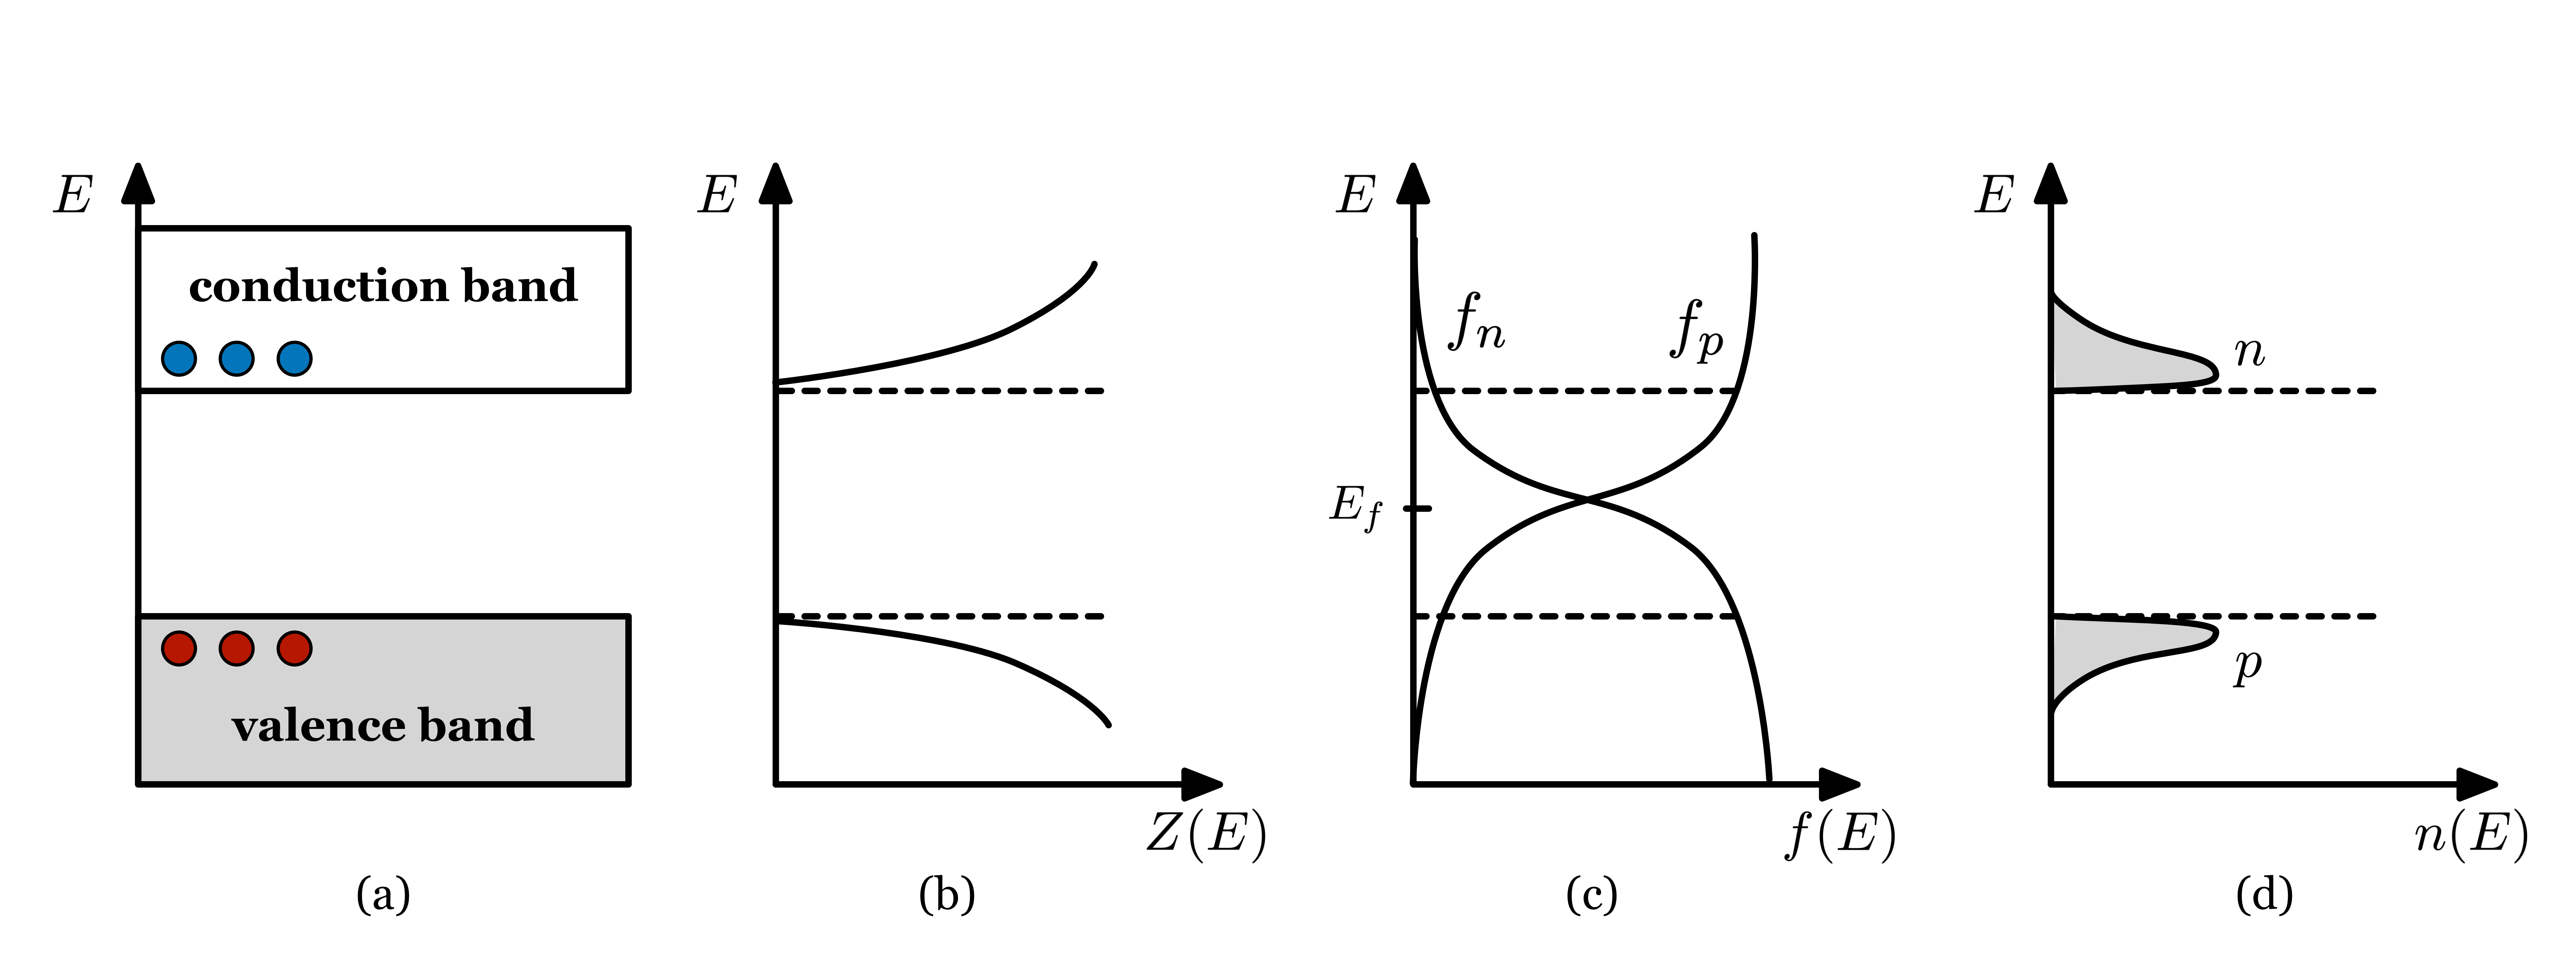
\includegraphics[width=0.95\linewidth]{files/band_diagram}
			\caption{Band diagram (a), Density of states (b), Occupation probabilities (c) and charge carrier densities (d)}
			% \label{ }
		\end{figure}

		For intrinsic semiconductors, a good approximation is to consider the Fermi energy level to be exactly in the middle of the band gap, this leads to having $(E-E_F) \gg kT$ and so  the expression for the occupation probabilities can be simplified as:
		\begin{equation}
			f_n(E) = \frac{1}{\exp(\frac{E-E_f}{kT}) + 1} \approx \exp(- \frac{E-E_f}{kT})
		\end{equation}

		It is then interesting to calculate the number densities $n$ and $p$ respectively for negative and positive charge carriers, integrating respectively over the conduction and valence band energies and using that by definition $f_n(E) + f_p(E) = 1$. This leads to: 
		\begin{equation}
			n = 2{\left( \frac{m_n^* kT}{2 \pi \hbar^2} \right)}^{3/2} \exp(-\frac{E_C - E_f}{kT}) \equiv N_C \exp(-\frac{E_C - E_f}{kT})
			\label{eq:ndensities_n}
		\end{equation}

		\begin{equation}
			p = 2{\left( \frac{m_p^* kT}{2 \pi \hbar^2} \right)}^{3/2} \exp(-\frac{E_f - E_V}{kT}) \equiv N_V \exp(-\frac{E_f - E_V}{kT})
			\label{eq:ndensities_p}
		\end{equation}

		For the sake of understanding, we can estimate the values of the effective densities of states, averaging over the effective masses of both charge carriers in Silicon and at room temperature (\SI{300}{\kelvin}) such that\ \cite{leroy2012silicon}: 
		\begin{equation}
			\begin{split}
				& N_C = 2 {\left( \frac{m_n^* kT}{2 \pi \hbar^2} \right)}^{3/2} \approx 3.05 \times 10^{19} \text{ cm$^{-3}$} \\
				& N_V = 2 {\left( \frac{m_p^* kT}{2 \pi \hbar^2} \right)}^{3/2} \approx 2.55 \times 10^{19} \text{ cm$^{-3}$}
			\end{split}
			\label{eq:effdensities}
		\end{equation}

		In thermal equilibrium, generation and recombination of electrons and holes respectively in the conduction and valence band are balanced which means: 
		\begin{equation}
			n = p = n_i \hspace{5mm} \Rightarrow \hspace{5mm} n \cdot p = n_i^2 = const
			\label{eq:massaction}
		\end{equation}

		In the case of unbalance between the number of positive and negative charge carriers (doping for instance could produce such an effect), we can use the expressions found in \eqref{eq:ndensities_n} and \eqref{eq:ndensities_p} to find: 
		\begin{equation}
			\begin{split}
				n_i^2 = np 	& = N_C N_V \exp(-\frac{E_C-E_V}{kT})\\
										& = N_C N_V \exp(-\frac{E_G}{kT})
			\end{split}
		\end{equation}
		The intrinsic carrier concentration depends on the difference of the energy levels of the conduction and valence band, the band gap energy, and has a dependence on the temperature such that: 
		\begin{equation}
			n_i \propto T^{3/2} \exp(\frac{-E_G}{2kT})
		\end{equation}
		Using the previously computed values for the effective densities of states in the conduction and valence band in \ref{eq:effdensities}, we find that at room temperature: 
		\begin{equation}
			n_i \approx 1.01 \times 10^{10} \text{ cm$^{-3}$}
		\end{equation}

		It is finally possible to give an expression to the Fermi level as a function of the energy levels of the conduction and valence bands and the effective masses fo electrons and holes, using that the concentration of both is equal: 
		\begin{equation}
			E_f = \frac{E_C + E_V}{2} + \frac{3kT}{4} \ln(\frac{m_p^*}{m_n^*})
		\end{equation}
		This results confirms that at $T =$ \SI{0}{\kelvin}, the Fermi level is exactly at the middle of the band gap and then slowly drifts away with increasing temperature due to the different in effective masses for electrons and holes. 
		To conclude the discussion on the electrical properties of intrinsic semiconductors, it is interesting to use the mobility of electrons and holes (respectively $\mu_e = $ \SI{1450}{\frac{\centi\meter\squared}{\volt\second}} and $\mu_h = $ \SI{500}{\frac{\centi\meter\squared}{\volt\second}}) to estimate the conductivity of intrinsic Silicon at room temperature: 
		\begin{equation}
			\sigma_i = n_i e {\left( \mu_e + \mu_h \right)} \approx 2.8 \times 10^{-4} \text{ ($\Omega$m)$^{-1}$}
		\end{equation}

		\subsubsection{Doping: extrinsic semiconductor}

		Extrinsic semiconductor are characterized by the addition of so-called impurities in the crystal's structure, the idea behind this doping of intrinsic semiconductors is to modify its conduction properties. Silicon being a tetravalent atom, it is possible to create an excess of electrons by replacing Silicon atoms by pentavalent atoms like Phosphorus (P) or Arsenic (As), these atoms are called donors.  Vice versa, it is possible to create an excess of holes by replacing Silicon atoms with trivalent atoms like Boron (B) or Gallium (Ga), these atoms are called acceptors.
		
		The mass-action law described in \eqref{eq:massaction} holds for doped semiconductors as the doping both increases the density of one type charge carrier and reduces the density of the other. Accounting for the fact that the net charge density of charge carriers for any volume element of semiconductor is zero, we obtain for the charge carrier densities as a function of the number of donor and acceptor atoms: 
		\begin{equation}
			\rho = e(n - p + N_A - N_D) = 0 \hspace{5mm} \Rightarrow \hspace{5mm} n-p = N_D - N_A
		\end{equation}
		
		Combining this relation to the mass-action law given in \eqref{eq:massaction}, one can derive the majority carrier densities and minority carrier densities in the cases in which electron (n-type semiconductor) or holes (p-type semiconductor) are dominating, respectively: 
		\begin{equation}
			n_n = \frac{1}{2} {\left( N_D - N_A + \sqrt{4 n_i^2 + (N_D - N_A)^2} \right)} \approx |N_D - N_A| \approx N_D
		\end{equation}
		\begin{equation}
			p_p = \frac{1}{2} {\left( N_A - N_D + \sqrt{4 n_i^2 + (N_D - N_A)^2} \right)} \approx |N_A - N_D| \approx N_A
		\end{equation}

		Equivalently, we can derive the minority carrier densities for holes and electrons respectively: 
		\begin{equation}
			p_n \approx \frac{n_i^2}{N_D - N_A} \approx \frac{n_i^2}{N_D} \hspace{5mm} ; \hspace{5mm} n_p \approx \frac{n_i^2}{N_A - N_D} \approx \frac{n_i^2}{N_A}
 		\end{equation}

		In n-type semiconductors, the addition of donor atoms for example will add some energy levels available slightly below the conduction band energy level so that new states will need to be accounted for in the density of states distribution. The Fermi level will then be raised from its intrinsic value $E_f$ to $E_F$ so that the population densities will change in favour of the electrons in the conduction band such that: 
		\begin{equation}
			n \approx N_D = N_C \exp(-\frac{E_C - E_f}{kT})\exp(-\frac{E_f - E_F}{kT}) = n_i \exp(-\frac{E_f - E_F}{kT})
		\end{equation}

		Equivalently, for p-type semiconductors: 
		\begin{equation}
			p \approx N_A = n_i \exp(\frac{E_f- E_F}{kT})
		\end{equation}
		The variation between the Fermi levels in the intrinsic and extrinsic cases is directly linked to the amount of donor or acceptors atoms. 
		Non desired impurities can also be present inside the crystalline structure as well as it is not straight forward to obtain a pure Silicon sample. Similarly, some different energy levels can be added and depending on their location in the band gap, they could act either as donors or acceptors.
		\clearpage
		\subsection{Junction and external voltage}\label{subsec:2.1.2}

		\begin{figure*}[h]
		\begin{minipage}{0.53\linewidth}
			A pn junction is created when bringing together p-type semiconductor and n-type semiconductor in contact. For the p-type side, the Fermi level is closer to the valence whereas for the n-type side, the Fermi level is closer to the conduction band. At the interface, the strong gradient in charge carrier concentration give rise to a diffusion current $I_{diff}$ such that electrons from the n-type side diffuse in the p-type side and vice versa for holes. Due to recombination of both charge carrier types around the interface, a zone free of space charge is generated: the depletion zone. The ionised donor and acceptors atoms are still present in the lattice and an intrinsic electrical field will be generated, resulting in a drift current $I_{drift}$ in opposition to the diffusion current. 	
		\end{minipage}\hfill
		\begin{minipage}{0.45\linewidth}
			\centering
			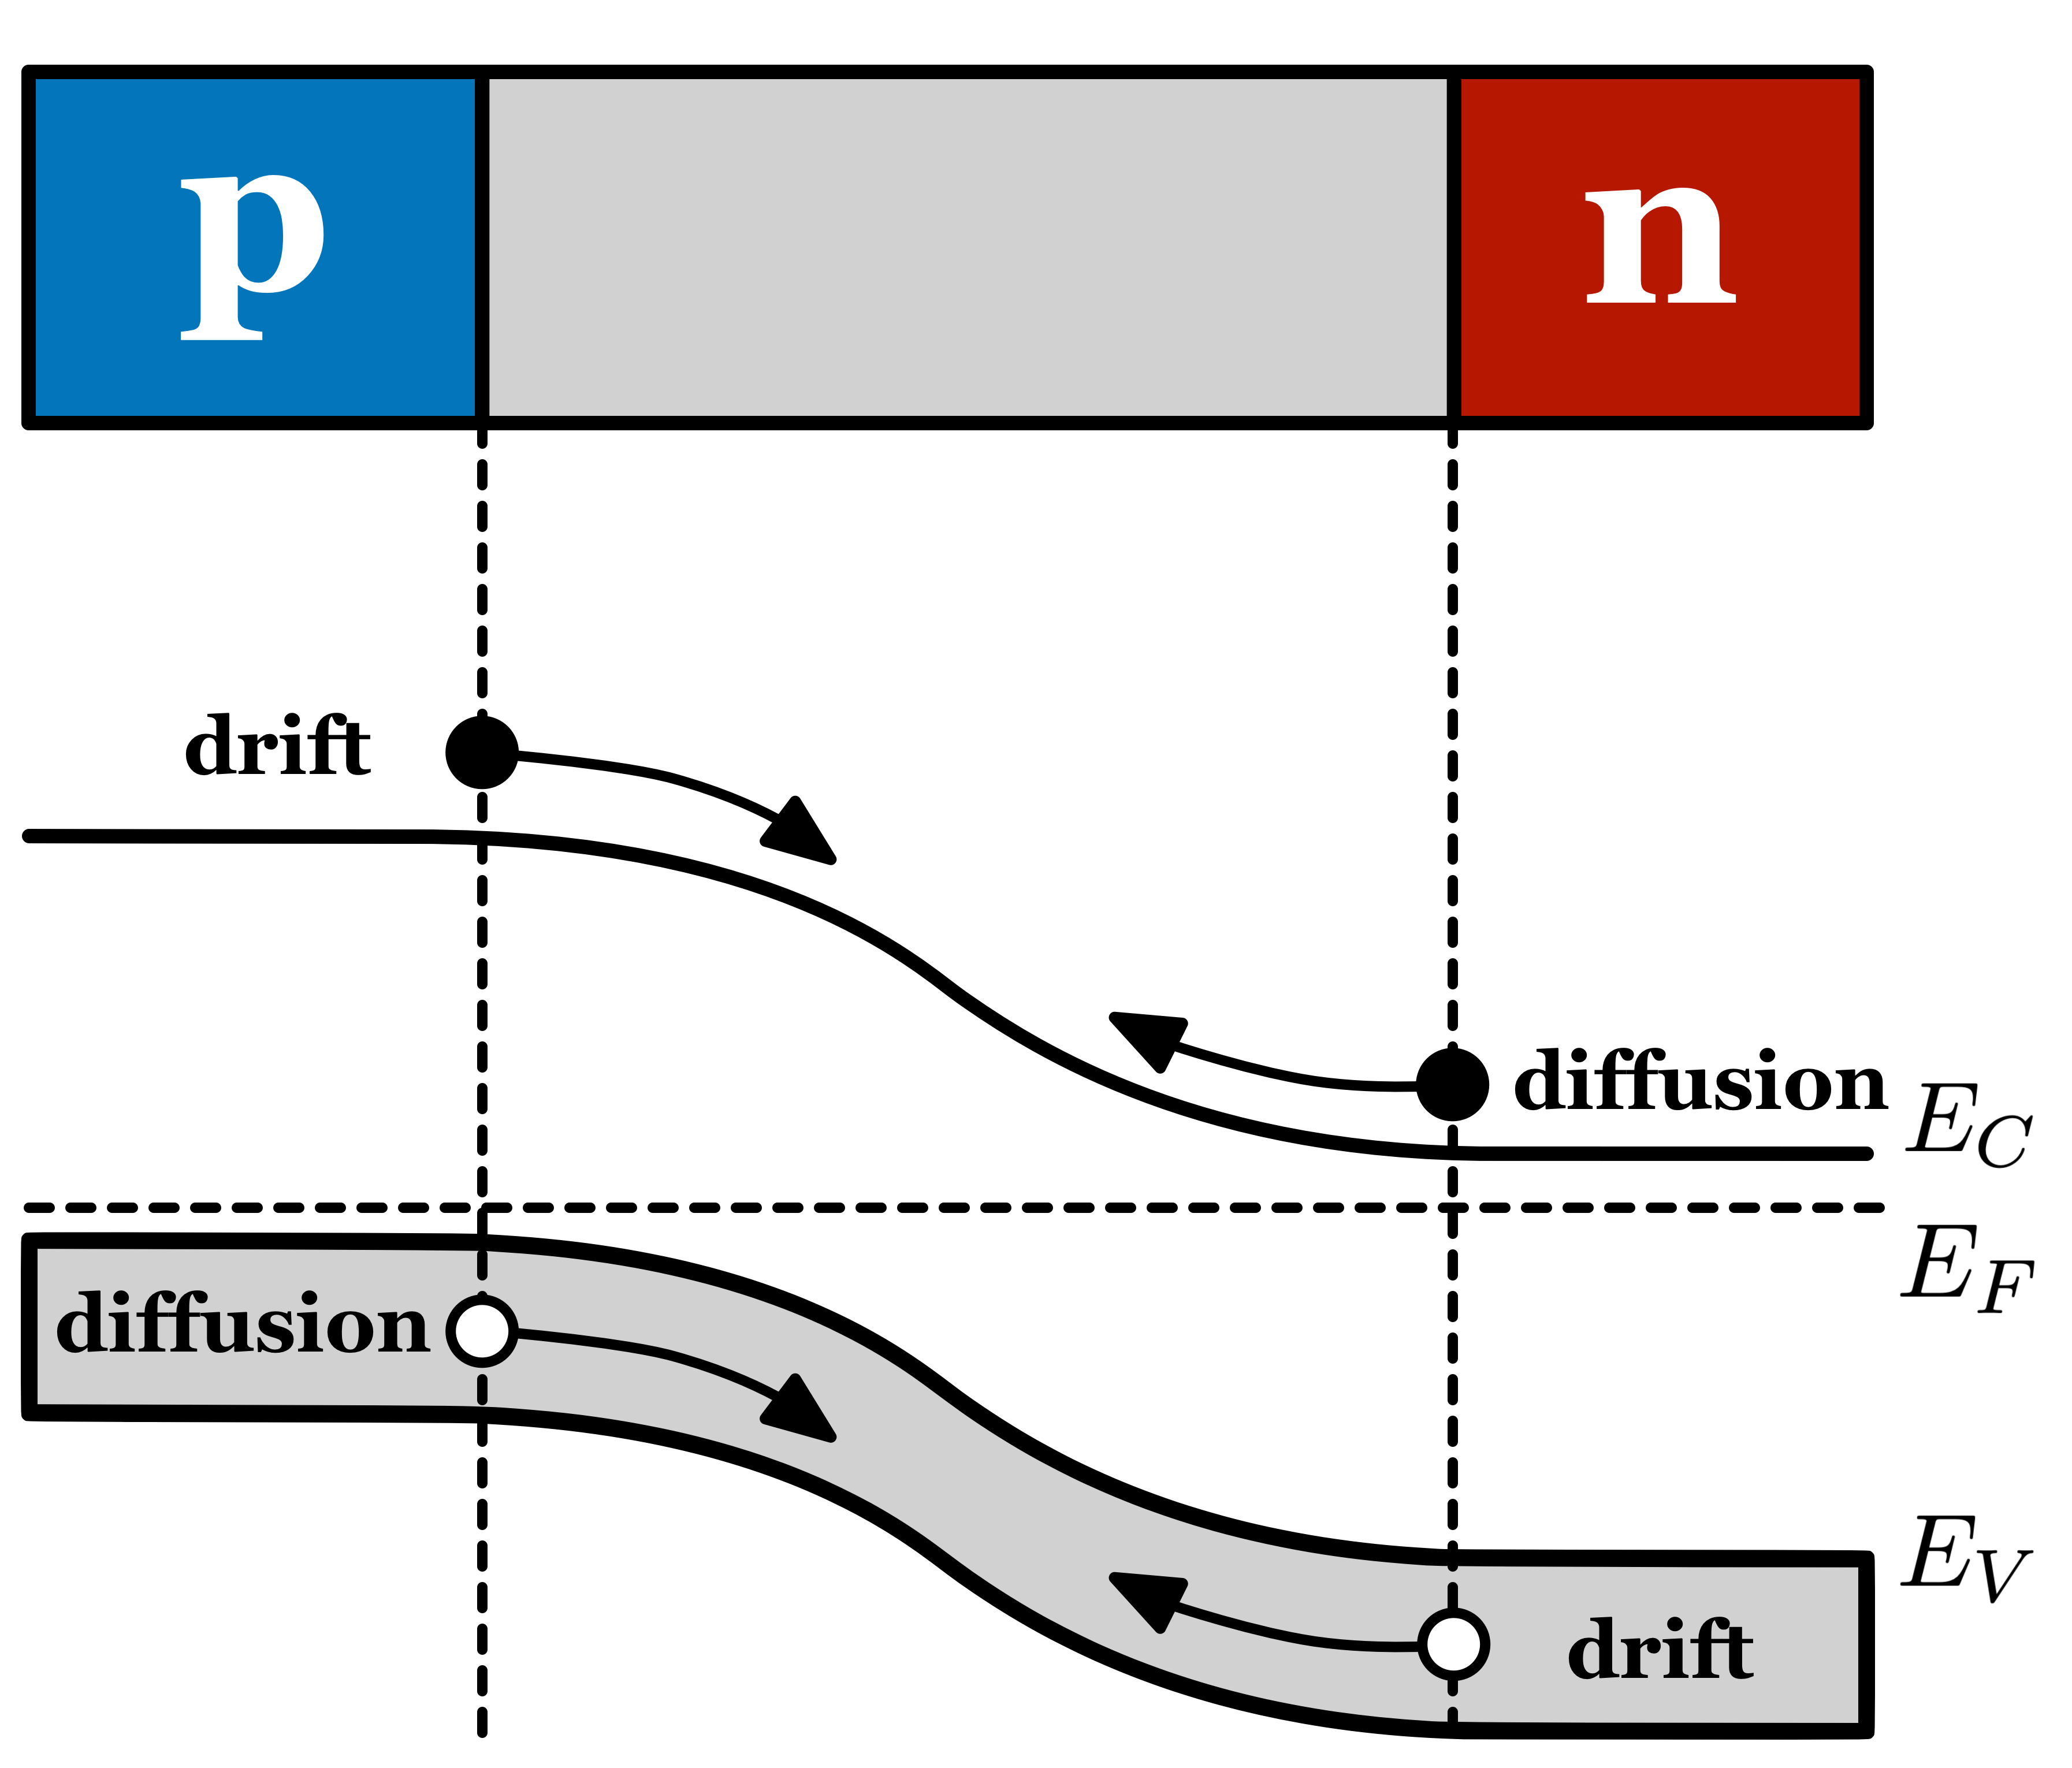
\includegraphics[width=1.0\linewidth]{files/band_structure}
			\caption{Band structure, potential and electric field of pn junction }
			\label{ }
		\end{minipage}
		\end{figure*}
		
		The resulting built-in electrical potential ($V_{bi}$) will produce a bending of the energy levels of the valence band and conduction band across the depletion region while the Fermi level will remain constant by its definition. 
		In equilibrium, the charge density can be written as: 
		\begin{equation}
			\rho(x) = 
			\begin{cases}
				-eN_A, & \text{for } -x_p < x < 0 \\
				+eN_D, & \text{for } 0 < x < x_n
			\end{cases}
		\end{equation}

		From the above equation and the neutrality condition $N_A x_p = N_D x_n$, one can derive the expression of the electric field $\mathcal{E}(x)$, imposing that the field has to be zero at the boundaries defined by $x_p$ and $x_n$ such that: 
		\begin{equation}
			\frac{d\mathcal{E}(x)}{dx} = \frac{\rho(x)}{\epsilon \epsilon_0} \hspace{4mm} \Rightarrow \hspace{4mm} \mathcal{E}(x) = 
			\begin{cases}
				\frac{-eN_A}{\epsilon \epsilon_0} (x + x_p) & \text{for } -x_p < x < 0 \\
				\frac{+eN_D}{\epsilon \epsilon_0} (x - x_n) & \text{for } 0 < x < x_n
			\end{cases}
			\label{eq:intrinsicEfield}
		\end{equation}

		By definition, the field maximum $\mathcal{E}_{max}$ is found at $x=0$. The built-in voltage can be derived through the integration of the intrinsic electric field obtained in \eqref{eq:intrinsicEfield} in the range defined by $x_p$ and $x_n$: 
		\begin{equation}
			\begin{split}
				V_{bi} = - \int_{-x_p}^{x_n} \mathcal{E}(x)dx &= \frac{e}{2 \epsilon \epsilon_0} (N_A x_p^2 + N_D x_n^2) \\
																											&= \frac{e}{2 \epsilon \epsilon_0} x_p^2 \frac{N_A}{N_D}(N_A + N_D)
			\end{split}
		\end{equation} 
		
		A useful definition of the built-in potential is through the difference in potential in the $n$ region $\phi_n$ and $p$ region $\phi_n$ around the depletion zone $V_{bi} = \phi_p - \phi_n$. The potential itself can be defined as the difference of extrinsic Fermi level $E_F$ and intrinsic Fermi level $E_f$ in both regions, such that:		 
		\begin{equation}
			\begin{split}
				V_{bi}  &= \phi_n - \phi_p = \frac{kT}{e}\ln(\frac{N_A}{n_i}) +\frac{kT}{e}\ln(\frac{N_D}{n_i})\\
								&=  \frac{kT}{e}\ln(\frac{N_A N_D}{n_i^2})
			\end{split}
			\label{eq:built-inpot}
		\end{equation} 

		To conclude this discussion it is interesting to compute the position of the boundaries of the depletion zone $x_n$ and $x_p$ as a function of the built-in potential and the donor and acceptor densities: 
		\begin{equation}
			x_p = \sqrt{\frac{2 \epsilon \epsilon_0}{e} V_{bi} \frac{N_D}{N_A(N_D + N_A)}} \hspace{5mm} \text{and} \hspace{5mm} x_n = \sqrt{\frac{2 \epsilon \epsilon_0}{e} V_{bi} \frac{N_A}{N_D(N_D + N_A)}}
		\end{equation}
		We observe that the depletion region is larger in the side of the junction where the doping is the lightest. Usually, the difference in doping concentrations is such that one can neglect for n-type (p-type) the density of donors (acceptors) and hence simplify the expression above. 

		\subsubsection{Effect of external voltage}
		
		Under equilibrium conditions, the width of the depletion zone is proportional to the amount of donor and acceptor atoms in the two sides of junctions but also to the built-in voltage generated from the movement of charge carrier within the junction. Although, if one was to apply an external difference in voltage $V_{ext}$ at the edges of the junction, the system would no longer be in equilibrium and charge carriers would start to move depending on the polarity of the voltage itself. We can hence consider the two following situations: 
		\begin{itemize}
			\item \textit{Forward-bias}: The applied external voltage $V_{ext}$ is negative on the n-side with respect to the p-side, more electrons will diffuse from the n-side to the p-side and vice versa for holes. The result is a reduction in the built-in potential and hence a reduction in the width of the depletion zone and a weaker bending of the energy bands. 
			\item \textit{Reverse-bias}: The applied external voltage $V_{ext}$ is positive on the n-side with respect to the p-side, more electrons will be removed from the n-side and vice versa for holes. The result is an increase in built-in potential and hence an increase in the width of the depletion zone and a stronger bending of the energy bands. 
		\end{itemize} 

		\begin{figure}[h]
		\centering
		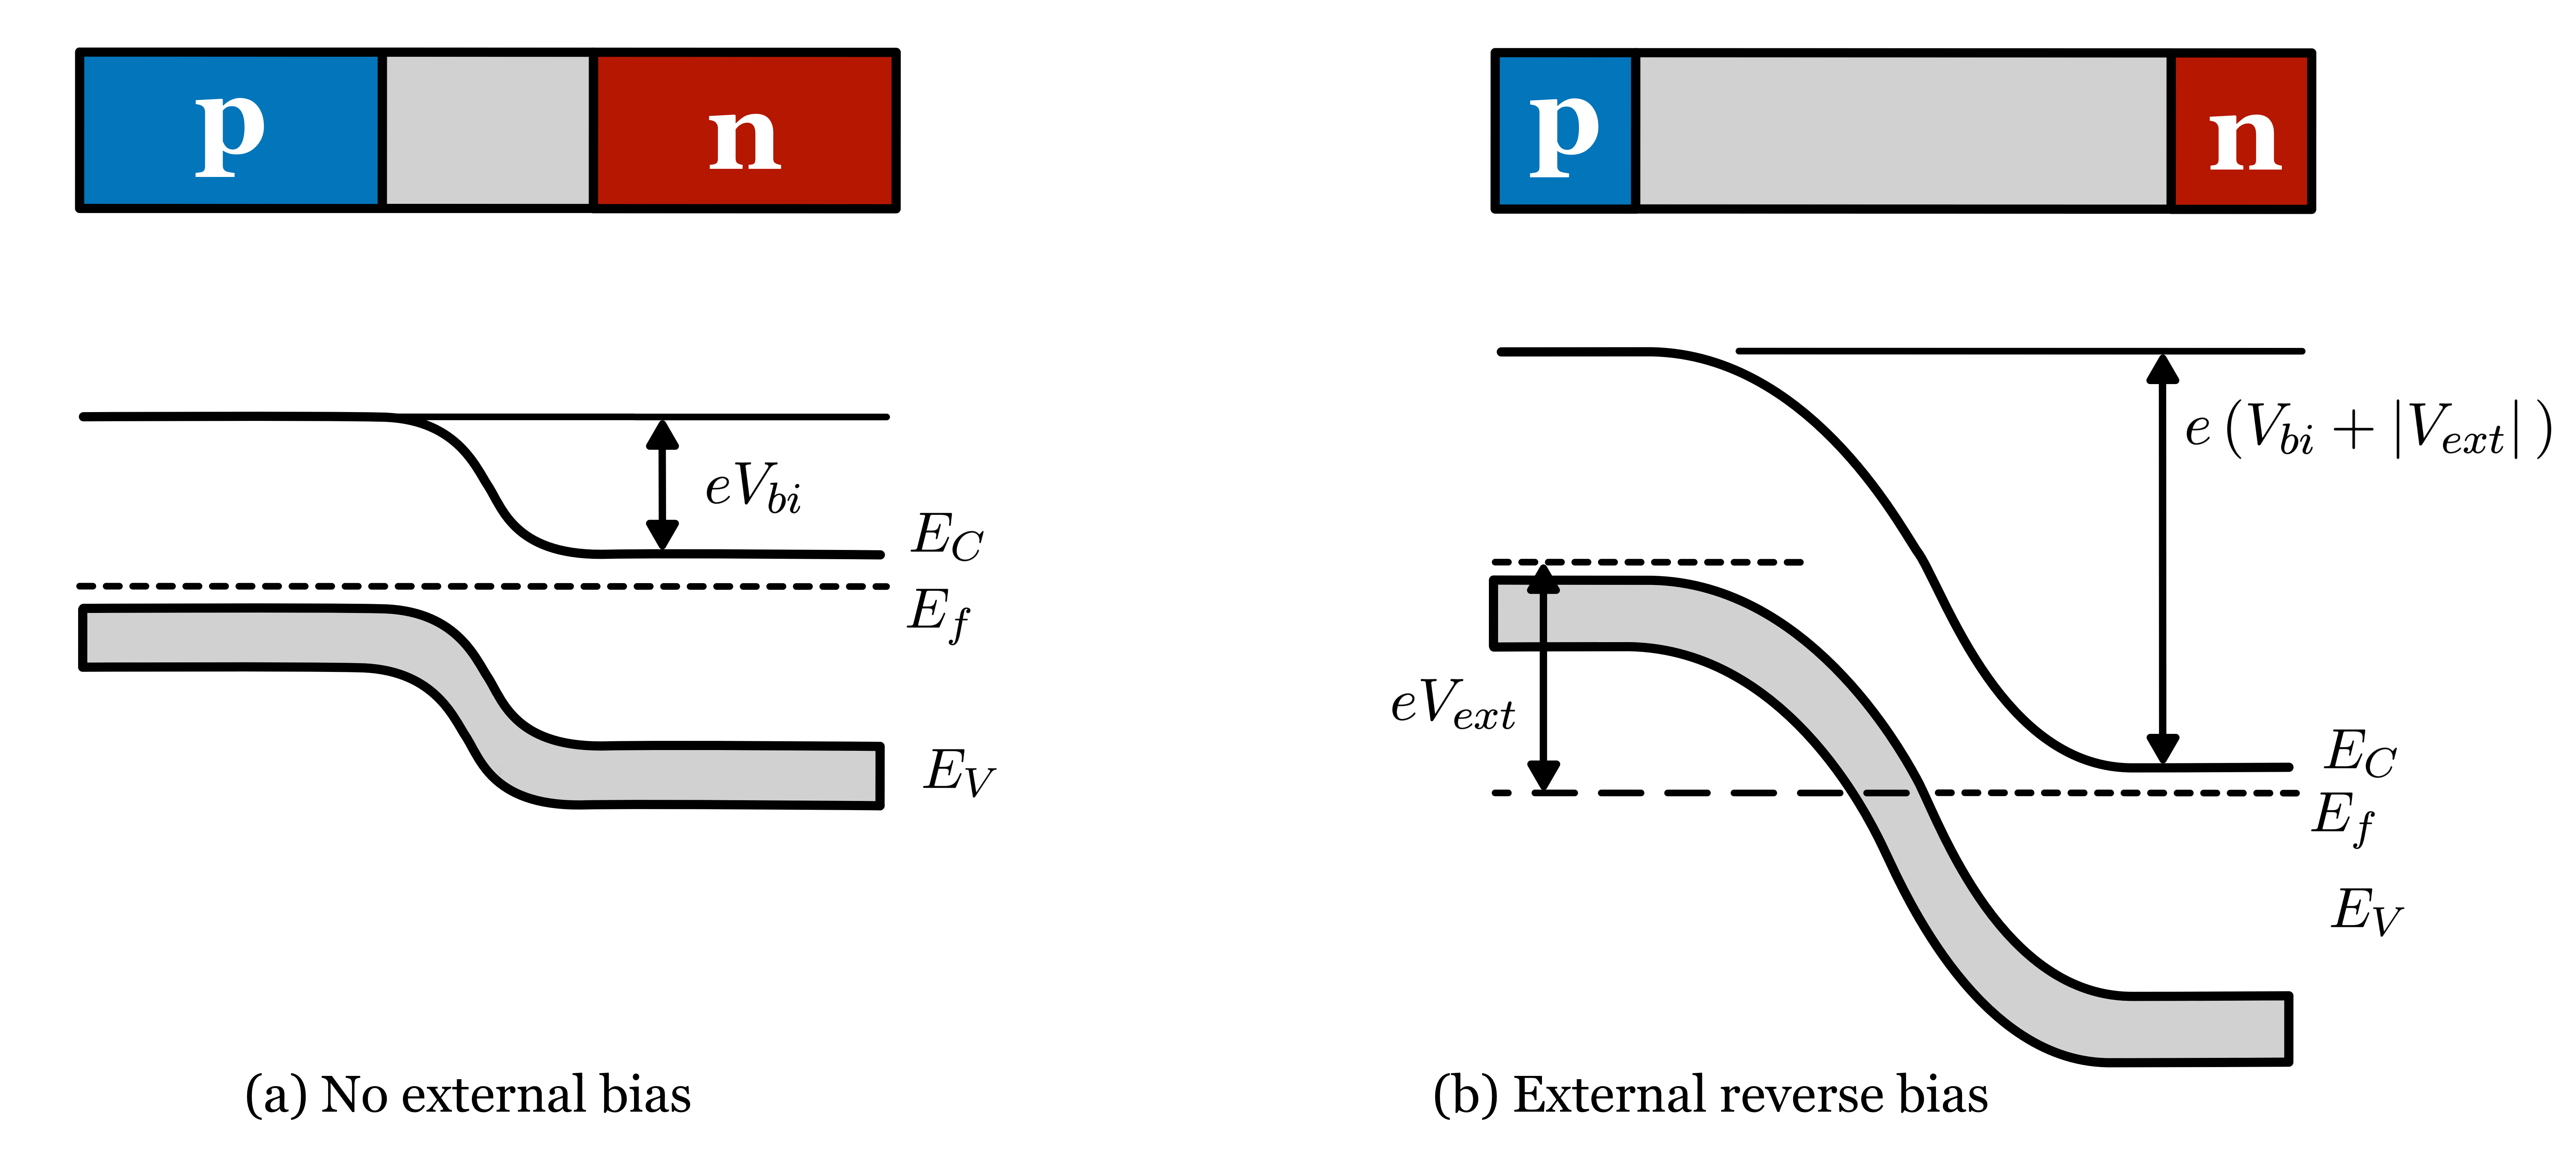
\includegraphics[width=1.0\linewidth]{files/pn_external_voltage}
		\caption{Effect of external voltage on a pn junction's band structure}
		\label{ }
		\end{figure}

	Outside the depletion region, equilibrium conditions hold and the concentration of majority carriers can be given by the donor and acceptor concentrations $N_A$ and $N_D$. 
	\clearpage
	Using the mass-action law, the expression for the built-in voltage from \eqref{eq:built-inpot} can then be adapted such that: 
	\begin{equation}
		V_{bi} = \frac{kT}{e} \ln(\frac{N_A N_D}{n_i^2}) \approx \frac{kT}{e} \ln(\frac{p_{p, eq} n_{n, eq}}{n_i^2}) = \frac{kT}{e} \ln(\frac{n_{n, eq}}{n_{p, eq}}) = \frac{kT}{e} \ln(\frac{p_{p, eq}}{p_{n, eq}})
	\end{equation}
	We have in the above equations defined the majority carrier concentrations in the n-side and p-side regions respectively as $n_{n, eq} \approx N_D$ and $p_{p, eq} \approx N_A$ and also the minority charge carriers, in the n-side and p-side regions, respectively as $n_{p, eq}$ and $p_{n, eq}$. One can first express the majority carrier densities in the region outside the space-charge region and then assume that these later are defined at the space charge boundaries by the difference $V_{bi} - V_{ext}$, such that: 
	\begin{equation}
		n_n(x = x_n) = n_p \exp(\frac{e(V_{bi} - V_{ext})}{kT}) \approx n_{n, eq}
	\end{equation}
	\begin{equation}
		p_p(x = -x_p) = p_n \exp(\frac{e(V_{bi} - V_{ext})}{kT}) \approx p_{p, eq}
	\end{equation}
	It is then possible to express this time the concentration of electrons at the boundary of the space-charge region on the p-side and the hole concentration at the opposite boundary on the n-side so that one obtains: 
	\begin{equation}
		n_p(x = -x_p) = n_{p, eq} \exp(\frac{e V_{ext}}{kT})
	\end{equation} 
	\begin{equation}
		p_n(x = x_n) = p_{n, eq} \exp(\frac{e V_{ext}}{kT})
	\end{equation}

	While reversed-bias is applied to the junction, the concentration of the majority charge carriers drop well below the minority charge carriers concentration in equilibrium and can be easily neglected in situation with high reversed-bias applied. Throughout the depletion region, the carrier concentration decreases from the majority carrier value $p_p (n_n)$ on one side, down to the minority carrier value $p_n (n_p)$ on the other side. The functional progression of the concentration into the depletion zone is determined by the concentration values at the end of the depletion region, that is, the transition to neutral regions. In summary, they are determined by the donor and acceptor concentrations and the external voltage applied to the junction\ \cite{detectors} 

	As it was discussed previously for the junction under no external voltage, it is possible to compute the depletion width of depletion zone and understand how it is affected. Respectively for the depletion zone boundary on the n-side or p-side, one obtains: 
	\begin{equation}
		d_{n} \approx x_n \approx \sqrt{\frac{2 \epsilon \epsilon_0}{e} \frac{1}{N_D}(V_{bi} - V_{ext})} \hspace{5mm} ; \hspace{5mm} d_{p} \approx x_p \approx \sqrt{\frac{2 \epsilon \epsilon_0}{e} \frac{1}{N_A}(V_{bi} - V_{ext})}
	\end{equation}
	A more convenient expression of the depletion width is through the use of the wafer resistivity which can be approximated as $\rho \simeq (e \mu_{e,h} N_{N_(D,A)})$, such that we obtain: 
	\begin{equation}
		d_n \approx 0.55 \sqrt{\frac{\rho}{\Omega cm} \frac{V_{ext}}{V}} \mu m \hspace{5mm} ; \hspace{5mm} d_{p} \approx 0.32 \sqrt{\frac{\rho}{\Omega cm} \frac{V_{ext}}{V}}  \mu m
		\label{eq:depletion_width}
	\end{equation}

	The difference between the p-side and n-side is due to the difference in mobility of electrons and holes, in order to deplete for example a silicon detector with \SI{300}{\micro\meter} width and a substrate resistivity of $\rho = $ \SI{2}{\kilo\ohm\centi\meter}, an external reverse bias voltage of \SI{160}{\volt} would need to be applied. 
\clearpage
	\subsubsection{Junction capacitance and full depletion}
		
	It is possible to treat the junction with a zone free of charge carriers just like a plate capacitor filled with a dielectric. The capacitance of the junction can then be given as a function of the area $A$ of the section of the junction and $d$ the width of the depletion zone by the following equation: 
		\begin{equation}
			\frac{C}{A} = \frac{\epsilon \epsilon_0}{d}
		\end{equation}

	We have seen previously that the depletion zone width depends on the applied external voltage \eqref{eq:depletion_width}. If one was to measure the capacitance as a function of the external bias supplied to the junction, it would be possible to find the tension for which the junction is fully depleted, since the capacitance would then become constant, we call this tension the full depletion voltage. 
	\begin{figure*}[h]
		\centering
			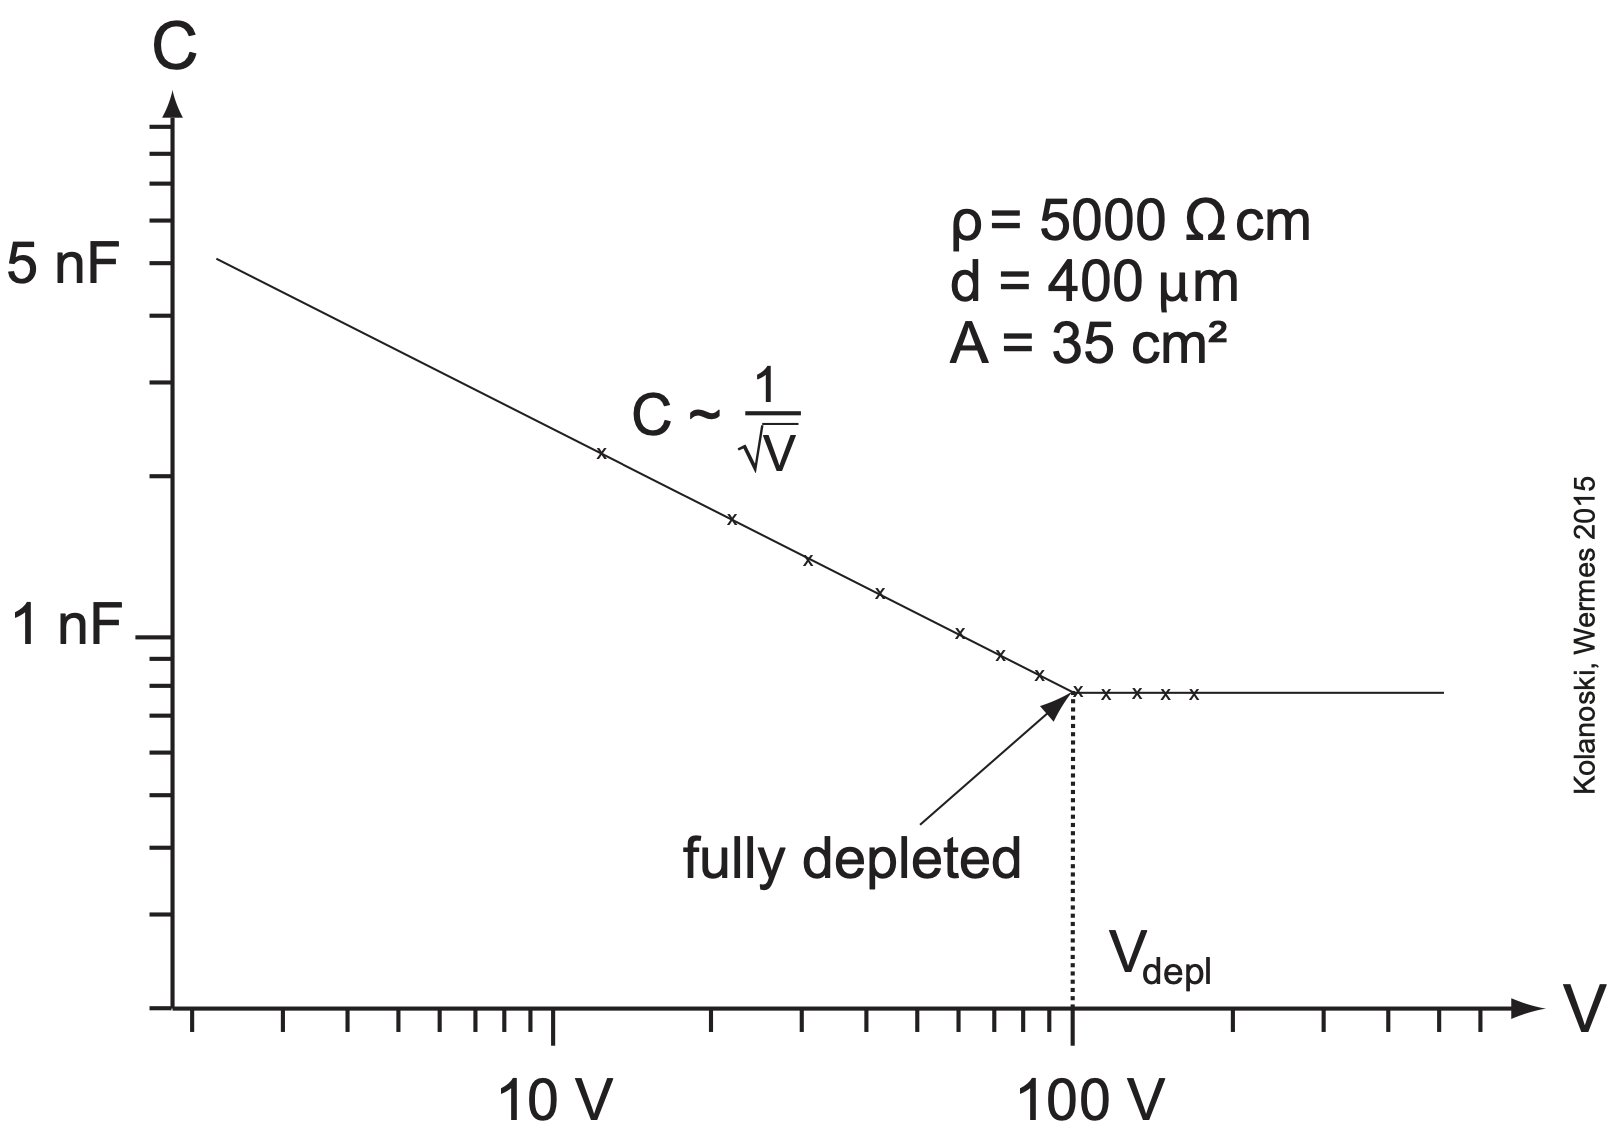
\includegraphics[width=0.6\linewidth]{files/CV_silicon}
			\caption{C-V curve of a silicon device in reverse bias}
			\label{ }
	\end{figure*}

	
	\clearpage
	\section{Signal formation and charge carrier transport}\label{sec:2.2}
		
	We previously discussed that it is possible to create with a pn junction, a region free of charge carriers, the so-called space charge region and that the width of this later can be adjusted by applying an external tension to the junction. While applying a reversed bias to the junction, one will increase the width of the space charge region. If a charged particle or a photon was to cross this region, some of the deposited energy would contribute to the creation of electron-hole ($e^- / h^+$) pairs. The energy required to generate a pair is temperature dependent but a commonly used value at room temperature is $\Delta E = \SI{3.6}{\electronvolt}$. Electrons and holes would then drift under the influence of the electric field inside the depletion region and could be collected on a readout electrode to observe the signal generated by the passage of this particle. 

	This is a very rough description of how semiconductors can be used for particle detection, in what follows we will give a more formal description of the drift of electrons and holes once they are generated, how the signal is induced at the electrodes and how the signal is formed.   

		\subsection{Drift of electrons and holes}\label{subsec:2.2.1}
		
		Motion of charges in semiconductors can be described by the Boltzmann transport equation as it takes into account both diffusion and drift mechanisms. Although, one also need to consider the lattice nature of semiconductors, implying that electrons and holes can be treated as if they were moving freely by using their effective mass as defined in \eqref{eq:effective_mass}. In semiconductors, the drift motion is a result of the acceleration of electrons and holes by the and electric field, moderated by friction and collision processes with the lattice phonon and impurities. The diffusion motion comes from the movement of charge carriers from a zone with lower concentration as it was discussed in \subsecref{subsec:2.1.2}

		For semiconductor particle detectors, the main process is the drift of electrons and holes induced by the external electric field induced by operating the devise in reversed-bias configuration. As said before, the motion can be described through the Boltzmann transport equation, but an often used description comes from using the Drude model \cite{Drude} which states that: 
		\begin{equation}
			m^* {\left( \dot{\vec{v}}_D + \frac{\vec{v}_D}{\tau}\right)} = q \vec{E}
		\end{equation} 
		We have here introduced as $\vec{v}_D$ the drift velocity and the various scattering effects are described by a relaxation parameter $\tau$, defined as the time separating two momentum changes between one scattering incidence and another. 
		
		\begin{figure*}[h]
			\centering
			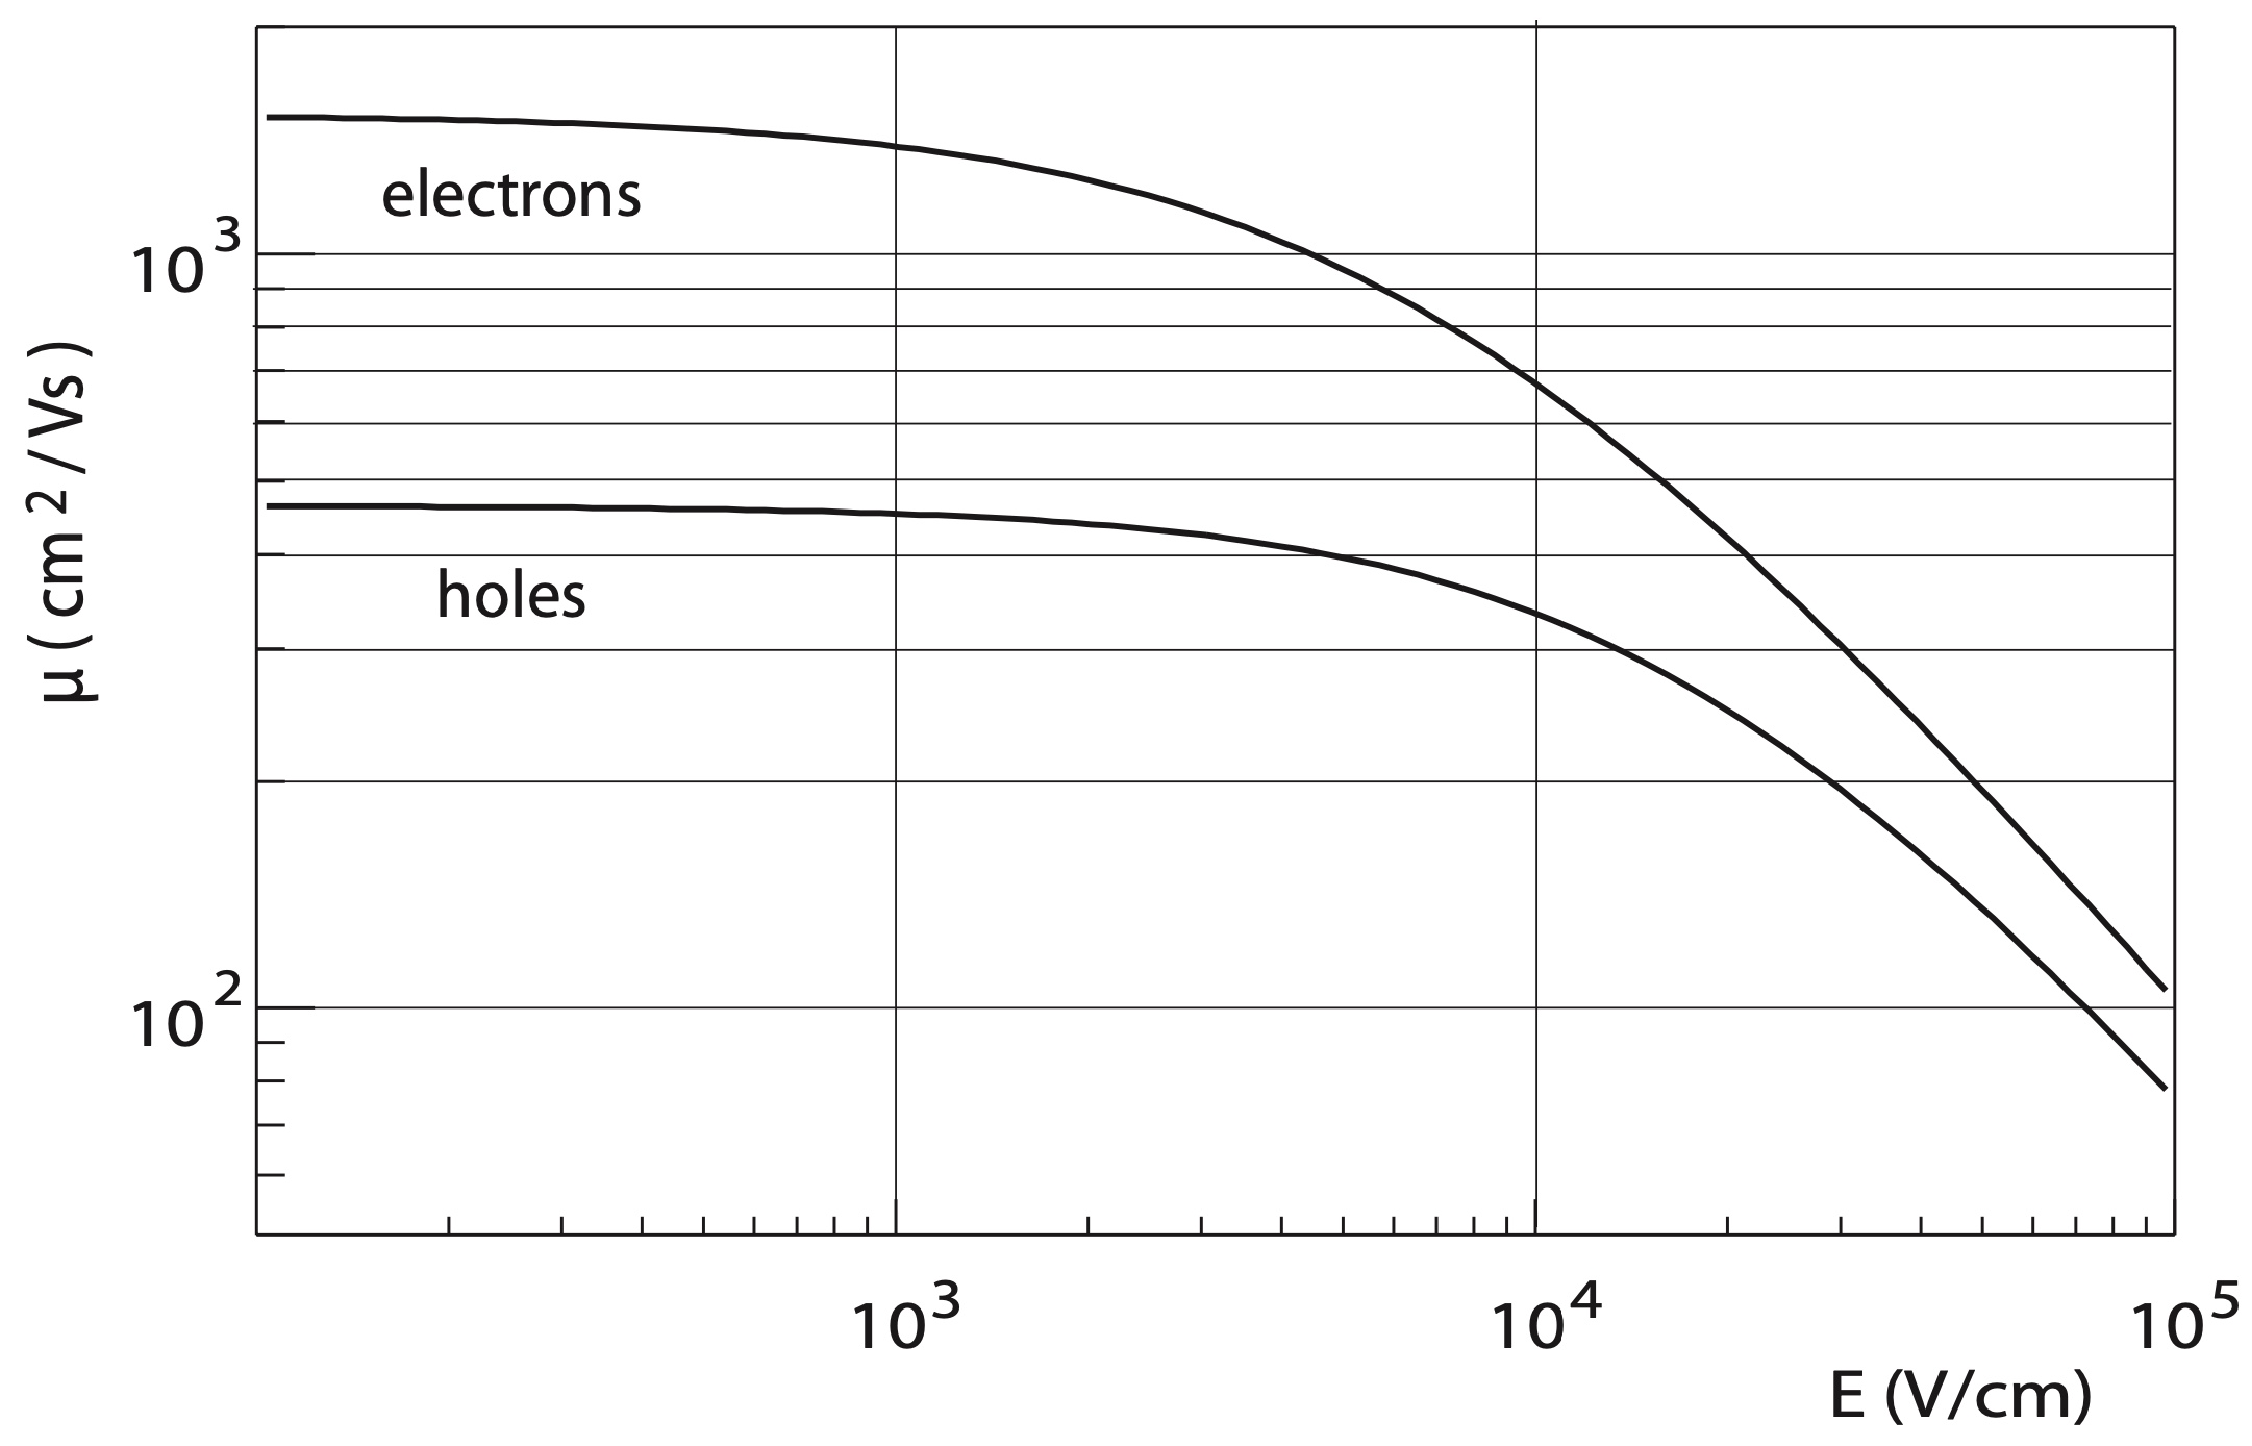
\includegraphics[width=0.58\linewidth]{files/electron-hole_mobility}
			\caption{ Mobilities of electron and holes in Silicon}
			\label{ }
		\end{figure*}

		If one assumes the stationary case of constant drift velocity, one can introduce the electron and hole mobility so that: 
		\begin{equation}
			\vec{v}_D = \frac{q \tau}{m^*} \vec{E} = \mu \vec{E} \hspace{5mm} \text{and} \hspace{5mm} \mu_{e,h} = \frac{q\tau}{m^*_{e,h}}
		\end{equation}
		
	
	

		The mobility of charge carriers is a temperature dependent quantity because of the temperature dependence of the different collisions processes defining the collision time $\tau$. As mentioned before, we can distinguish the collisions involving acoustic phonons (coherent lattice oscillations) for which the mobility decreases for increasing temperature, and the collisions involving impurities in the lattice, for which the mobility increases (weakly decreases) for collisions with charged (neutral) impurities.  

		The mobility of charge carriers also depends on the electric field present within the depletion region, at low electric fields ($E \ll \SI{10}{\kilo \volt \per \centi\meter}$), the drift velocity is proportional to the electric field whereas at high electric fields, the mobility is field dependent. At low electric field, thermal equilibrium can be assumed and the emission and absorption of phonons by charge carriers lead to almost no deviation from the proportionality to the electric field. With increasing electric field, a stationary equilibrium is reached between the energy spent for the acceleration of the charge carriers and the energy transferred to the lattice phonon scattering, the drift velocity eventually becomes constant (for Silicon at least). A sufficiently simple empirical ansatz gives a good description of the drift's velocity dependence on the electric field\ \cite{drift_velocity_vs_E}: 
		\begin{equation}
			\vec{v}_D = \mu(E) \vec{E} = \frac{\mu_0}{{\left(1 + {\left( \frac{\mu_0 E}{v_{sat}} \right)^\beta}\right)^{1/\beta}}} \vec{E}
			\label{eq:drift_velocity}
		\end{equation}
		We have here introduced $\mu_0$ the mobility at low electric field values, $v_{sat}$ the saturated drift velocities reached for high electric fields and an empirical constant $\beta$ which is usually taken to be 2 for electrons and 1 for holes in Silicon \cite{beta_drift_velocity}.  
		
		\begin{figure*}[h]
			\centering
			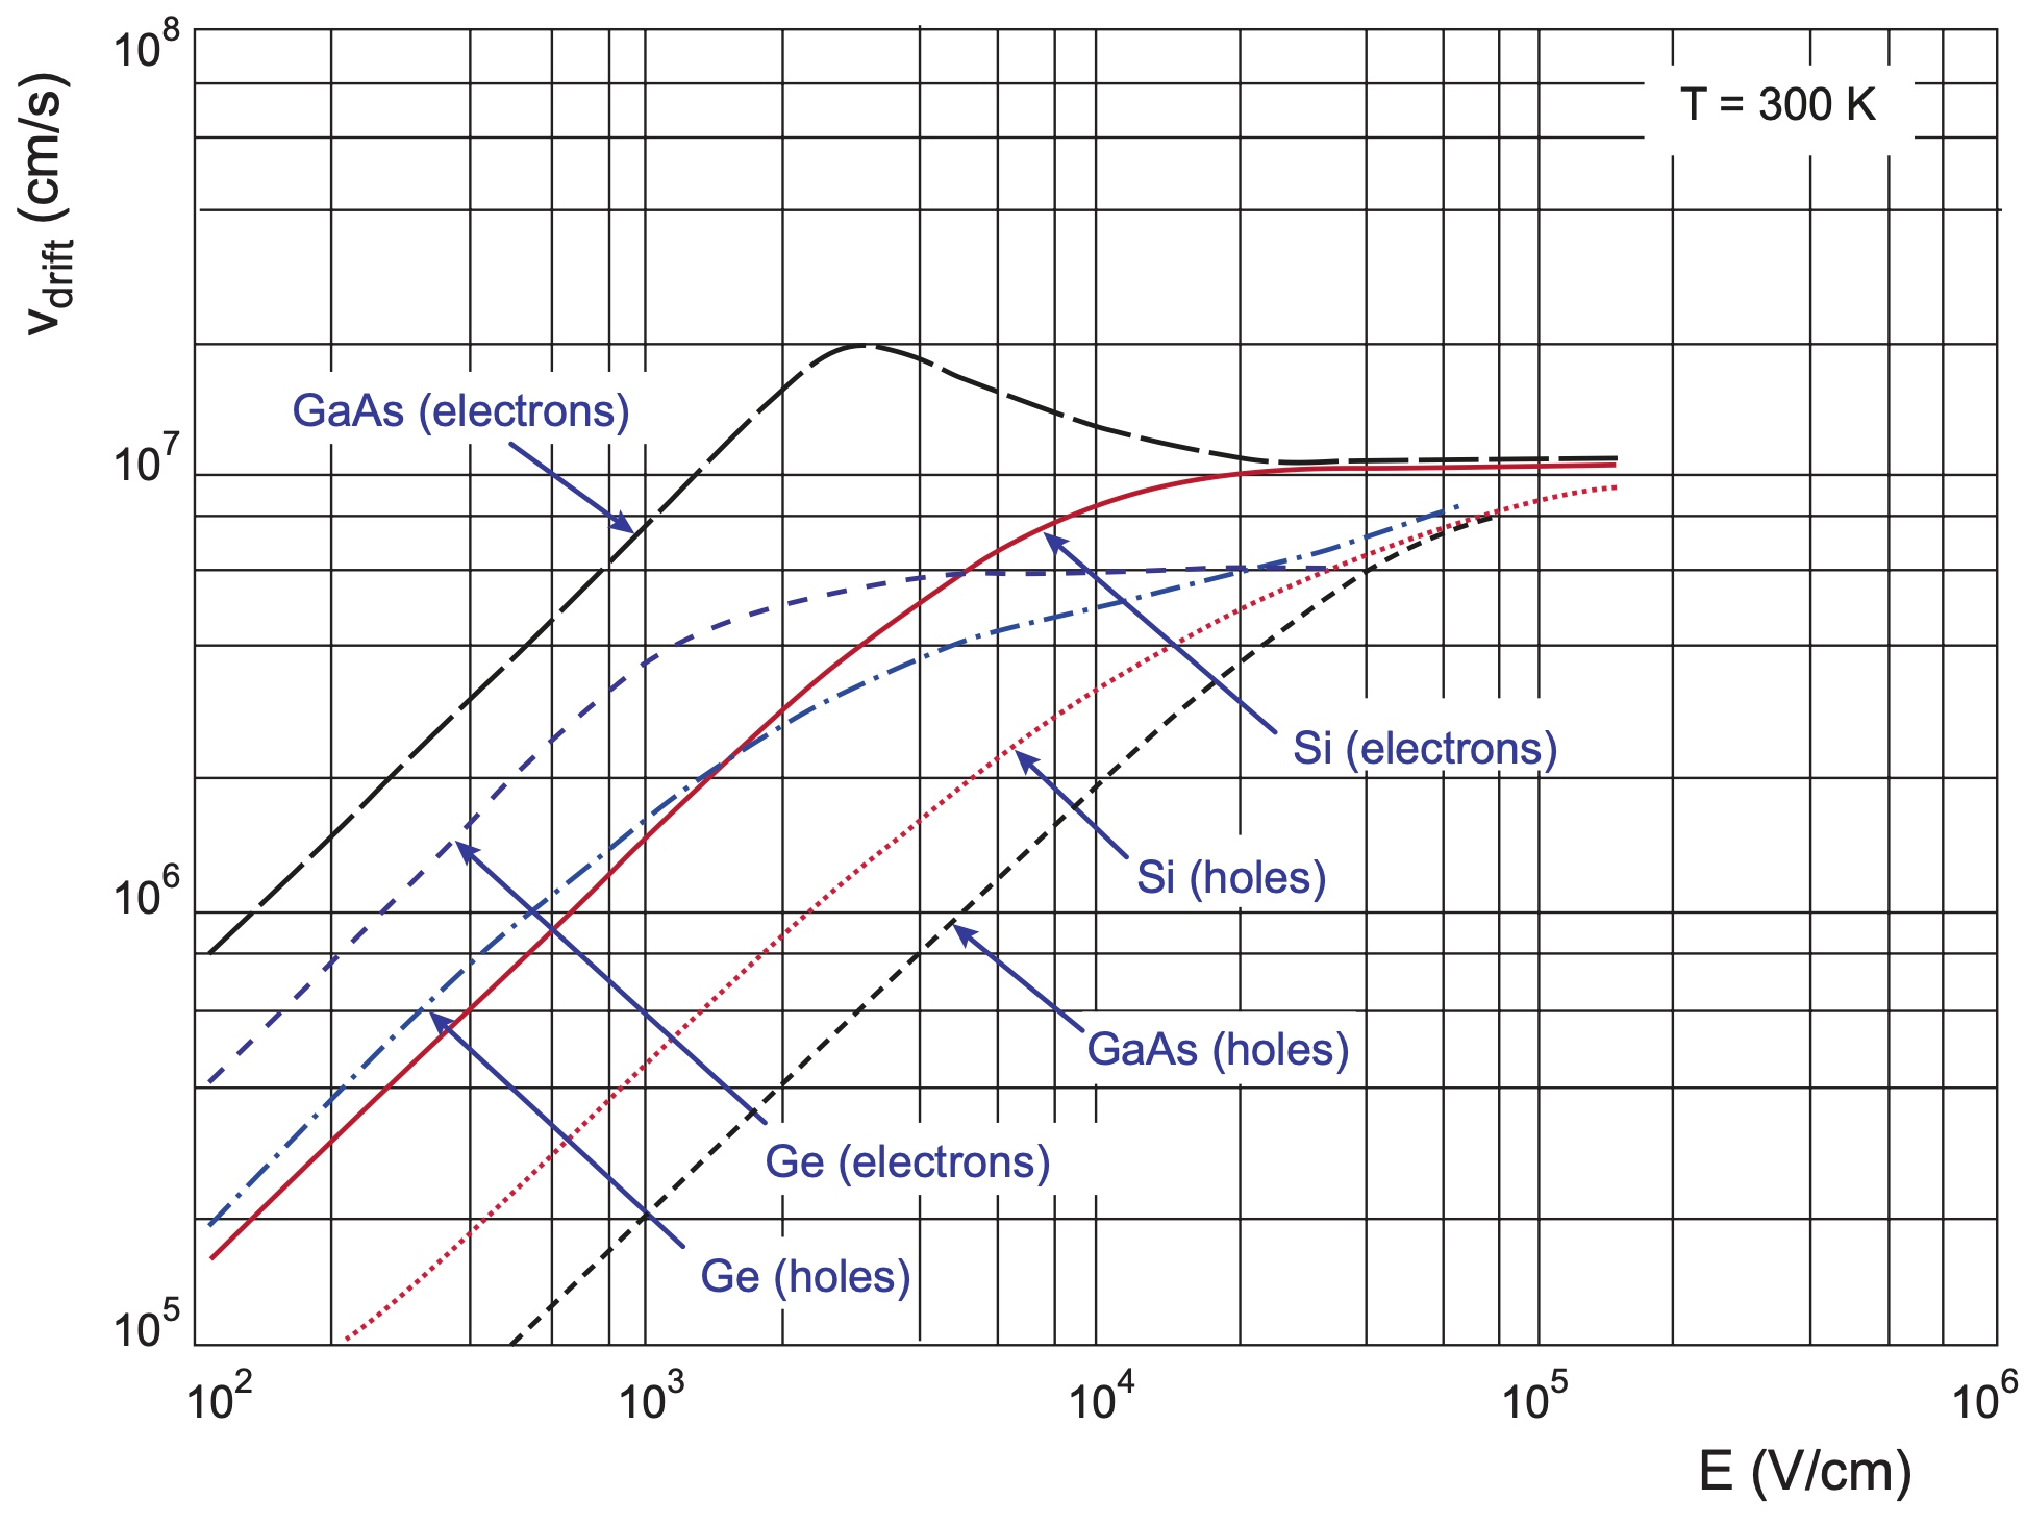
\includegraphics[width=0.6\linewidth]{files/electron-hole_driftvelocity}
			\caption{ Drift velocities for different semiconductor materials}
			\label{ }
		\end{figure*}
		
		
		
	

		The saturated drift velocity usually reaches a value of $v_{sat} \approx 10^7$ cm/s at room temperature. The low field conditions mobilities for Silicon can also be calculated at room temperature and one would obtain: 
		\begin{equation}
			\mu_n = 1450\ \frac{\text{cm}^2}{\text{Vs}} \hspace{5mm} ; \hspace{5mm} \mu_p = 500\ \frac{\text{cm}^2}{\text{Vs}} \approx \frac{1}{3} \mu_n
		\end{equation} 

		\subsection{Weighting field and Shockley-Ramo theorem}\label{subsec:2.2.2}
		Having characterised the motion of charge carriers inside the depletion region of a semiconductor particle detector, it is interesting to understand what is the mechanism describing the induction of a signal on the electrodes of the said detector. Before going any further into the discussion, it is fundamental to understand that the charges induced at the electrodes does not require collection of the generated charge in the detector volume through ionisation. Indeed, while moving, the generated charge will induce an accumulation of charges on the surface of the electrodes.
		\begin{figure}[h]
		\centering
		\includegraphics[width=0.7\linewidth]{files/two_electrode_shockleyramo}
		\caption{Two electrode configuration for signal induction by moving charge}
		\label{im:ShockleyRamo}
		\end{figure}
		In order to give a comprehensive description of the formation of signals by moving charges we will discuss a simple example in which single charge is moving between two electrodes, one at a potential $V$ and the other one set to ground. The movement of the charge will lead to a charge induction $+Q$ and $-Q$ on the electrodes, if we assume that the system has capacitance $C$, the charge induced by the potential difference $V$ is hence $Q = CV$. The moving charge $q$ located at $\vec{r}_q$ will induce an additional charge $\Delta Q(\vec{r}_q)$ and while moving from a position $\vec{r}_q$ to $\vec{r}_q + d\vec{r}_q$, the field $\vec{E}_0$ on the electrodes will produce a work such that: 
		\begin{equation}
			dW_q = q\vec{E}_0 d\vec{r}_q
		\end{equation}
		The work has to be delivered either by the power supply $W_V$ or by the field energy $W_E$. If the voltage at the electrode is kept constant, the work performed by the power supply is then only determined by the extracted charge $dQ$ from the supply itself so that:
		\begin{equation}
			\begin{split}
				dW_q + dW_V + dW_E 	&= dW_q + (dQV + QdV) + dW_E\\
				 										&= dW_q + dQV  + dW_E = 0
			\end{split}
		\end{equation}
		The convention is to have $dQ < 0$ if the charge moved into the power supply is negative and vice versa, $dQ$ always has the opposite sign as the charge induced in the electrode's surface. The total field energy in the volume $\tau$ defined by the electrodes is given by: 
		\begin{equation}
			W_E = \frac{\epsilon \epsilon_0}{2} \int_{\tau} \vec{E}^2 d\tau
		\end{equation}
		The total electric field $\vec{E}$ can be expressed using the superposition principle as shown in figure \ref{im:ShockleyRamo} with the first component $\vec{E}_0$ is the field generated by the electrodes and $\vec{E}_q$ is the field generated by the moving charge alone. The corresponding potential $\phi{\vec{r}}$ can also be decomposed into the component $\phi_0$ without the moving charge and the potential generated by the moving charge itself $\phi_q(\vec{r})$. Summarised all together we obtain: 
		\begin{equation}
			\vec{E} = \vec{E}_0 + \vec{E}_q \hspace{5mm} \text{and} \hspace{5mm} \phi(\vec{r}) = \phi_0(\vec{r}) + \phi_q(\vec{r})
		\end{equation}
		The potential $\phi_0(\vec{r})$ and $\phi_q(\vec{r})$ respectively have to satisfy the Poisson and Laplace equation with the following boundary conditions at the inner and outer electrodes: 
		\begin{equation}
			\begin{cases}
				&\Delta \phi_0 = 0 \\
				&\Delta \phi_q = -\frac{q}{\epsilon \epsilon_0} \delta(\vec{r} - \vec{r}_q)
			\end{cases}
			\hspace{5mm} \text{with} \hspace{5mm}
			\begin{cases}
				&\phi(\vec{r})|_{inner}\ = \phi_0({\vec{r}})|_{inner} = V \\
				&\phi(\vec{r})|_{outer}\hspace{1.8mm} = \phi_0({\vec{r}})|_{outer} = 0 \\
				&\phi_q(\vec{r})|_{inner} = \phi_q({\vec{r}})|_{outer} = 0 \\
			\end{cases}
		\end{equation}
		The electric field respectively corresponding to these potentials are given by: 
		\begin{equation}
			\vec{E}_0 = - \vec{\nabla} \phi_0 \hspace{5mm} \text{and} \hspace{5mm} \vec{E}_q = - \vec{\nabla} \phi_q
		\end{equation}
		It is possible to show thanks to Green's theorem, that the field energy of the static electrode field can be split into the two components from the electrodes themselves and the point charge \cite{Shockley–Ramo}. Since we assumed the field $\vec{E}_0$ to be static because of the constant voltage and since the field $\vec{E}_q$ will generate no work either on the charge itself nor with the power supply, the energy contribution of these two field do not change under the movement of the charge, so that: 
		\begin{equation}
			W_E = W_{E_0} + W_{E_q}  \hspace{5mm} ; \hspace{5mm} dW_E = dW_{E_0} + dW_{E_q} = 0
		\end{equation}
		We arrive to the conclusion that the work exerted on the moving charge is solely provided by the voltage source so that we obtain: 
		\begin{equation}
			dW_q + dW_V = q \vec{E}_0 d\vec{r} + dQ V = 0 \hspace{5mm} \Rightarrow \hspace{5mm} dQ = -q \frac{\vec{E}_0}{V} d\vec{r}
		\end{equation}
		The electric field $\vec{E}_0$ is proportional to the tension applied at the electrodes $V$ so that the induced charge $dQ$ in the above equation is independent on the tension at the electrodes. We can hence define the so-called weighting field and weighting potential by setting the electrode tension to $V=1$ such that: 
		\begin{equation}
			\phi_w = \frac{\phi_0}{V} \hspace{5mm} \text{and} \hspace{5mm} \vec{E}_w = - \vec{\nabla} \phi_w
		\end{equation}
		The weighting field is then a quantity that is only dependent on the geometry of the electrodes and defines the path the generated charges will follow inside the detector, it has by definition the units of inverse length. One can also derive the time evolution of the induced charge giving rise to the signal's current defined as: 
		\begin{equation}
			i_S = -\frac{dQ}{dt} = q \vec{E}_w \vec{v}_D\hspace{5mm} \text{and} \hspace{5mm} \vec{v}_D = \frac{d\vec{r}}{dt} 
			\label{eq:ShockleyRamo}
		\end{equation} 
		The last two equations are the simplification of the Shockley-Ramo theorem in the case of a detector with two electrodes only. The result is fundamental and tells us that the shape of the induced current does not directly depend on the strength of the electric field between the electrodes but also on the geometry of the detector itself. The electric field usually defines the direction and the velocity of the drifting charges, indeed we have seen that the drift velocity of charge carriers depend on the electric field as described by \eqref{eq:drift_velocity}. The weighting field is not per se a physical field but describes how the movement of a charge carrier will induce a signal on a given electrode, it is completely uncorrelated to the dynamics of the charge carriers. 
		\clearpage
		\subsection{Space charge and signal formation}\label{subsec:2.2.3}

		In the presence of space charge, just like it is the case for the depletion zone of semiconductor detectors, the weighting field should not be affected. Similarly to how we treated the presence of the moving charge, we can use the superposition principle to add the contribution of a density of charge such that the total potential becomes: 
		\begin{equation}
			\phi(\vec{r}) = \phi_0(\vec{r}) + \phi_q(\vec{r}) + \phi_\rho(\vec{r})
		\end{equation}
		This potential needs to solve the Laplace equation $\Delta \phi_\rho = -\frac{\rho}{\epsilon \epsilon_0}$ with the same boundary conditions used for the potential generated by the moving charge. Since the electrodes are grounded when adding the space charge density and since it is stationary, it leads to the conclusion that this additional potential does not contribute to the energy balance and so the weighting field. 

		On the contrary, the space charge density has an effect on the physical electric field, we will now see how to compute the signal induced on the electrodes of a semiconductor detector with geometry resembling the one of a parallel plate capacitor filled with a dielectric. In this configuration, the electric field is no longer constant and will decrease from the junction side to the opposite side of the detector. For the following discussion, we will follow the example given in \cite{detectors} and discuss a detector made of weakly doped n-type substrate $n^-$ on which a more strongly doped p-type layer ($p^+$) is applied. On the opposite side of the junction lays a strongly doped n-type layer ($n^+$) used as contact, while applying increasing reverse bias voltage, the depletion layer grows into the detector.

		Once full depletion is reached, the electric field is null at the interface between $n^-$ and $n^+$ which corresponds to the opposite side of the position of the readout electrode on which the signal is induced. On the other hand, if the detector is not fully depleted (underpletion), the field becomes null within the undepleted layer whilst for higher potential than the full depletion potential (overdepletion), a constant field component is added to the linear component. A general expression for the electric field can be given as: 
		\begin{equation}
			\begin{split}
				\vec{E}_x &= - {\left[ \frac{2V_{dep}}{d^2} (d-x) + \frac{V-V_{dep}}{d} \right]} \vec{e}_x \\
									&=- {\left[ \frac{V + V_{dep}}{d} - \frac{2V_{dep}}{d^2}x \right]} \vec{e}_x 
			\end{split}
		\end{equation}

		We have defined here as $V$ the voltage applied to the edges of the detector, $V_{dep}$ the voltage required to reach full depletion and $d$ the thickness of the detector. Since the doping concentration is much weaker in the $n^-$ layer with respect to the $p^+$ layer, the depletion happens mostly inside the n-type layer. The full depletion voltage can then be written as a function of the density of donor atoms $N_D$ and the thickness $d$ following \eqref{eq:depletion_width} such that:
		\begin{equation}
			V_{dep} \approx \frac{eN_D}{\epsilon \epsilon_0}\frac{d^2}{2}
			\label{eq:depletion_voltage}
		\end{equation} 
		For further development, we will rewrite the electric field such that 
		\begin{equation}
			\vec{E}(x) = (bx-a)\vec{e}_x \hspace{5mm} \text{with} \hspace{5mm} a = \frac{V + V_{dep}}{d} \hspace{3mm} ; \hspace{3mm} b=\frac{2V_{dep}}{d^2}
		\end{equation}

		If we now were to consider a particle crossing the depletion layer and generating at position $x = x_0$ an electron-hole pair, the holes would drift in the direction of the field and the electrons in the opposite direction so that their respective velocities can be expressed as:
		\begin{equation}
			\begin{split}
				v_e &= -\mu_e E_x(x_e) = - \mu_e (bx_e-a) = - \frac{1}{\tau_e}{\left( x_e-\frac{a}{b} \right)} = \dot{x}_e \\
				v_h &= +\mu_h E_x(x_h) = + \mu_h (bx_h-a) = + \frac{1}{\tau_h}{\left( x-h-\frac{a}{b} \right)} = \dot{x}_h \\
			\end{split}
		\end{equation}

		We have introduced the constant $\tau{e,h}$, respectively the characteristics times for electron and hole movement which can be explicitly written as: 
		\begin{equation}
			\tau_{e,h} = \frac{1}{b \mu_{e,h}} = \frac{d^2}{2\mu_{e,h}V_{dep}}
		\end{equation}
		The time dependent solutions to the differential equations for the position of the electron and hole exhibit an accelerated movement of the charge carrier with a saturation of the drift velocity under high field conditions, they take the form:  
		\begin{equation}
			\begin{split}
				x_e(t) &= \frac{a}{b} - {\left( \frac{a}{b} -x_0 \right)} e^{-t/\tau_e} \hspace{4mm} ; \hspace{4mm} v_e(t) = \dot{x}_e = \frac{1}{\tau_e}{\left( \frac{a}{b} -x_0 \right)}e^{-t/\tau_e} \\
				x_h(t) &= \frac{a}{b} - {\left( \frac{a}{b} -x_0 \right)} e^{+t/\tau_h} \hspace{4mm} ; \hspace{4mm} v_h(t) = \dot{x}_h = -\frac{1}{\tau_h}{\left( \frac{a}{b} -x_0 \right)}e^{+t/\tau_h}
			\end{split}
		\end{equation}

		Under full depletion condition, the electrons will reach the electrode located at $x = d$ at a time $t = T^-$ and the holes will reach the electrode located at $x=0$ at a time $T^+$, their respective expression are: 
		\begin{equation}
			T^- = \tau_e \ln(\frac{a-bx_0}{a-bd}) \hspace{5mm} ; \hspace{5mm} T^+ = \tau_h \ln(\frac{a}{a-bx_0})
		\end{equation}
		It is interesting to note that the collection times are finite number under the condition that the denominator is strictly positive which implies that the voltage used to operate the detector has to be larger that the full depletion voltage. In the case in which the potential would be smaller than the full depletion voltage, the charge would not be collected. Ultimately we have shown that this is not a problem as long as the charge is not generated in a vanishing field region since the sole movement of the generated charge will induce a signal on the electrode. 
		
		It is now time to use the Shockley-Ramo theorem in order to compute what is the generated signal by the electron-hole pair on the top readout electrode. Beforehand, we need to find the expression for the weighting field, we have argued that in the presence of space charge, this later is not impacted and so for a parallel plate geometry its expression is: 
		\begin{equation}
			\vec{E}_w = - \frac{1}{d} \vec{e}_x
			\label{eq:weighting_field}
		\end{equation}
		Using the expression for the induced signal in \eqref{eq:ShockleyRamo} and the velocities of electrons and holes, it follows: 
		\begin{equation}
			\begin{split}
				i_S^e(t) &= \frac{e}{d\tau_e}{\left( \frac{a}{b} - x_0 \right)} e^{-t/\tau_e} \hspace{5mm} \text{for} \hspace{3mm} t < T^- \\
				i_S^h(t) &= \frac{e}{d\tau_h}{\left( \frac{a}{b} - x_0 \right)} e^{+t/\tau_h} \hspace{5mm} \text{for} \hspace{3mm} t < T^+
			\end{split}
		\end{equation}
		The validity domain of the equations is important as the signal will no longer be induced from the moment the charge will be collected at the electrode. We can rewrite the characteristic times for electrons and holes as a function of Silicon's relative permittivity and the density of donor atoms using \eqref{eq:depletion_voltage} so that it reads: 
		\begin{equation}
			\tau_{e,h} = \frac{d^2}{2 \mu_{e,h}V_{dep}} \approx \frac{\epsilon \epsilon_0}{\mu_{e,h} N_D}
		\end{equation}

		For Silicon, $\epsilon = 11.9$ and using a typical concentration of $N_D = 10^{12}$ cm$^{-3}$, we obtain for the characteristic times for electrons and holes respectively $\tau_e =$ \SI{5}{\nano\second} and $\tau_h =$ \SI{15}{\nano\second}. By assuming that the detector is operated in overdepletion so that the collection times are finite, one would find that the collection times do not exceed couple tenths of nanoseconds (depending on where the electron-hole pair is produced) \cite{detectors}, silicon based detectors can hence be implemented as fast detectors. 

		Finally, it is interesting to combine both current from the electron and holes to obtain the total induced current such that: 
		\begin{equation}
			\begin{split}
				i_S^{tot}(t) 	&= i_S^{e}(t) + i_S^{h}(t) \\
											&=\frac{e}{d} {\left( \frac{a}{b} -x_0\right)} {\left( \frac{1}{\tau_e}e^{-t/\tau_e}\Theta(T^- - t) + \frac{1}{\tau_h}e^{+t/\tau_h}\Theta(T^+ - t) \right)}
			\end{split}
		\end{equation}

		Integrating the total current, it is possible to obtain the expression for the induced charge signal such that: 
		\begin{equation}
			\begin{split}
				Q_S^{tot}(t) 	&= \int i_S^{tot}(t) dt \\
											&= -e \frac{a-bx_0}{bd} {\left[ {\left( 1- e^{-t/\tau_e}\right)\Theta(T^- - t)} + {\left( e^{+t/\tau_h} + 1  \right) \Theta(T^+ - t)} \right]} \\
											& -e \frac{a-bx_0}{bd} {\left[ {\left( 1- e^{-T^-/\tau_e}\right)\Theta(t - T^- )} + {\left( e^{+T^+/\tau_h} + 1  \right) \Theta(t - T^+)} \right]}
			\end{split}
			\label{eq:induced_charge}
		\end{equation}

		We have arranged the above equation in order to evidence the first part of the equation, corresponding to the growth of the induced charge while the charges generated in the depletion layer move and the second part of the equation, corresponding to the total induced charged once the generated charges have been collected. It is interesting to note that summing the total charge induced by the electron and the hole, we obtain exactly $Q_S^{tot} = -e $. 
		Accounting for a detector capacitance $C_D$ the signal charge can be converted into a voltage signal so that: 
		\begin{equation}
			v_S(t) = \frac{Q_S(t)}{C_D}
		\end{equation}
		We have started from the description of the movement of charge carriers with the depletion layer through drift due to the electric field, we have calculated how the movement of these charges can induce a current on the readout electrodes, and we finally have obtained the expression in terms of current, charge and voltage for the signal induced on the readout electrode of the semiconductor particle detector.
		\clearpage

	\section{Signal readout and processing}\label{sec:2.3}
	So far, we have been discussing how semiconductor can be used as a sensitive device to the passage of a particle through ionisation thanks to the pn junction. We have discussed the properties of such particle detectors as well as the mechanism behind the signal induction of the generated charges relative to the geometry of the detector itself and relative to the movement of the generated charges themselves. Another key aspect to the detection of particles is the way the signal is readout from the collection electrode and how it is later processed. In general detector readout systems are application specific and can be very different from one application to another. The aim of the subsequent discussion will be to give a general overview of the main component of a detector readout and then move towards more specific configurations used throughout this work. More detailed and complete descriptions will be given in the following chapters. (\note{cite the chapters or sections here}) 


		\subsection{Detector readout}\label{subsec:2.3.1}
		The passage of a particle through the sensitive part of a semiconductor detector generates an induced current $I_{ind}$ on the readout electrode, an electronic readout system is then required to acquire and process this current. The readout system is responsible for assigning through the induced signal a measure of Time of Arrival (ToA) of the particle and a measure of amplitude which can be then associated with dedicated calibrations to the amount of deposited energy or charge by the particle in the detector. Such a system is called readout electronics and can be split into an analog part, the front-end and the digital logic. A typical schematic view is given in the figure below:  
		\begin{figure}[h]
		\centering
		\includegraphics[width=0.9\linewidth]{files/general_electronics}
		\caption{Typical front-end readout scheme including amplification, shaping, and discrimination stage}
		\label{ }
		\end{figure}
		
		In semiconductor detectors, the signal charge is usually very small (in contrast to detector types which already amplify the deposited charge before reaching the electronic readout), an amplification stage called pre-amplifier is then needed. This is required so that the digital logic can later process the signal. The pre-amplifier is often built with a capacitive feedback loop of capacitance $C_f$ so that the pre-amplifier acts as an integrator of the induced current. 
		The output of this stage is a voltage step whose level is proportional to the signal in input by a factor $A_\nu$ defined as the gain of amplifier (later discussed in \note{add reference to dedicated subsection}). A shaping stage is usually (but not always) required to transform the voltage step input into a signal with return to baseline within a certain finite time, it acts as a filtering stage by limiting the bandwidth of the signal which also acts on electronic noise. (later discussed in \note{add reference to dedicated subsection}). 
		The analog signal then goes through a discrimination stage called discriminator which acts as a comparator between the analog signal's level and a fixed reference level also called threshold voltage $V_{thr}$. The output of the discriminator is a squared signal for which the length in time is equal to the time the analog signal's level is above the threshold voltage, also called Time Over Threshold (TOT). Once the signal becomes digital, it will be further process by the digital logic to measure the deposited charge or energy and a time of arrival. Many solutions with advantages and inconvenient exist and the architecture choices become very application specific. The particular configurations of the digital logic used in this work will later be presented more in details in the section dedicated to ASIC descriptions. (\note{add here relevant sections}). 
	

		\subsection{Amplification stage }\label{subsec:2.3.2}
		As mentioned previously, input charge from semiconductor detectors can be very small and usually in the range of femtocoulombs, hence an amplification stage is essential. The type of amplifier configuration depends on the sensor design and essentially affects the Signal to Noise Ratio (SNR) through a trade-off between noise and response time. For detectors with small input charge and small SNR, Charge Sensitive Amplifiers (CSAs) are the preferred solution. To fulfil the requirements of the different sensors presented in this work, the amplifiers used are implementing Bipolar Junction Transistors (BJTs) as transimpedance amplifiers (TIAs) but need to be operated under specific conditions providing them with properties similars to those of a CSA. We first start this discussion with an overview of how CSA function.   
		\begin{figure*}[h]
		\begin{minipage}{0.49\linewidth}
			We have discussed in \subsecref{subsec:2.2.3} that charge can be measured through the integration of the induced current $i_{S}$ over time as shown by \eqref{eq:induced_charge}. The CSA will then produce an output signal under the form of a step voltage whose level is proportional to the input charge. The CSA consists of an inverting Operational Amplifier (OpAmp) characterised by a high internal gain $A_\nu$ typically frequency dependent, together with a capacitive feedback loop responsible for the integration. 
		\end{minipage}\hfill
		\begin{minipage}{0.49\linewidth}
		\centering
		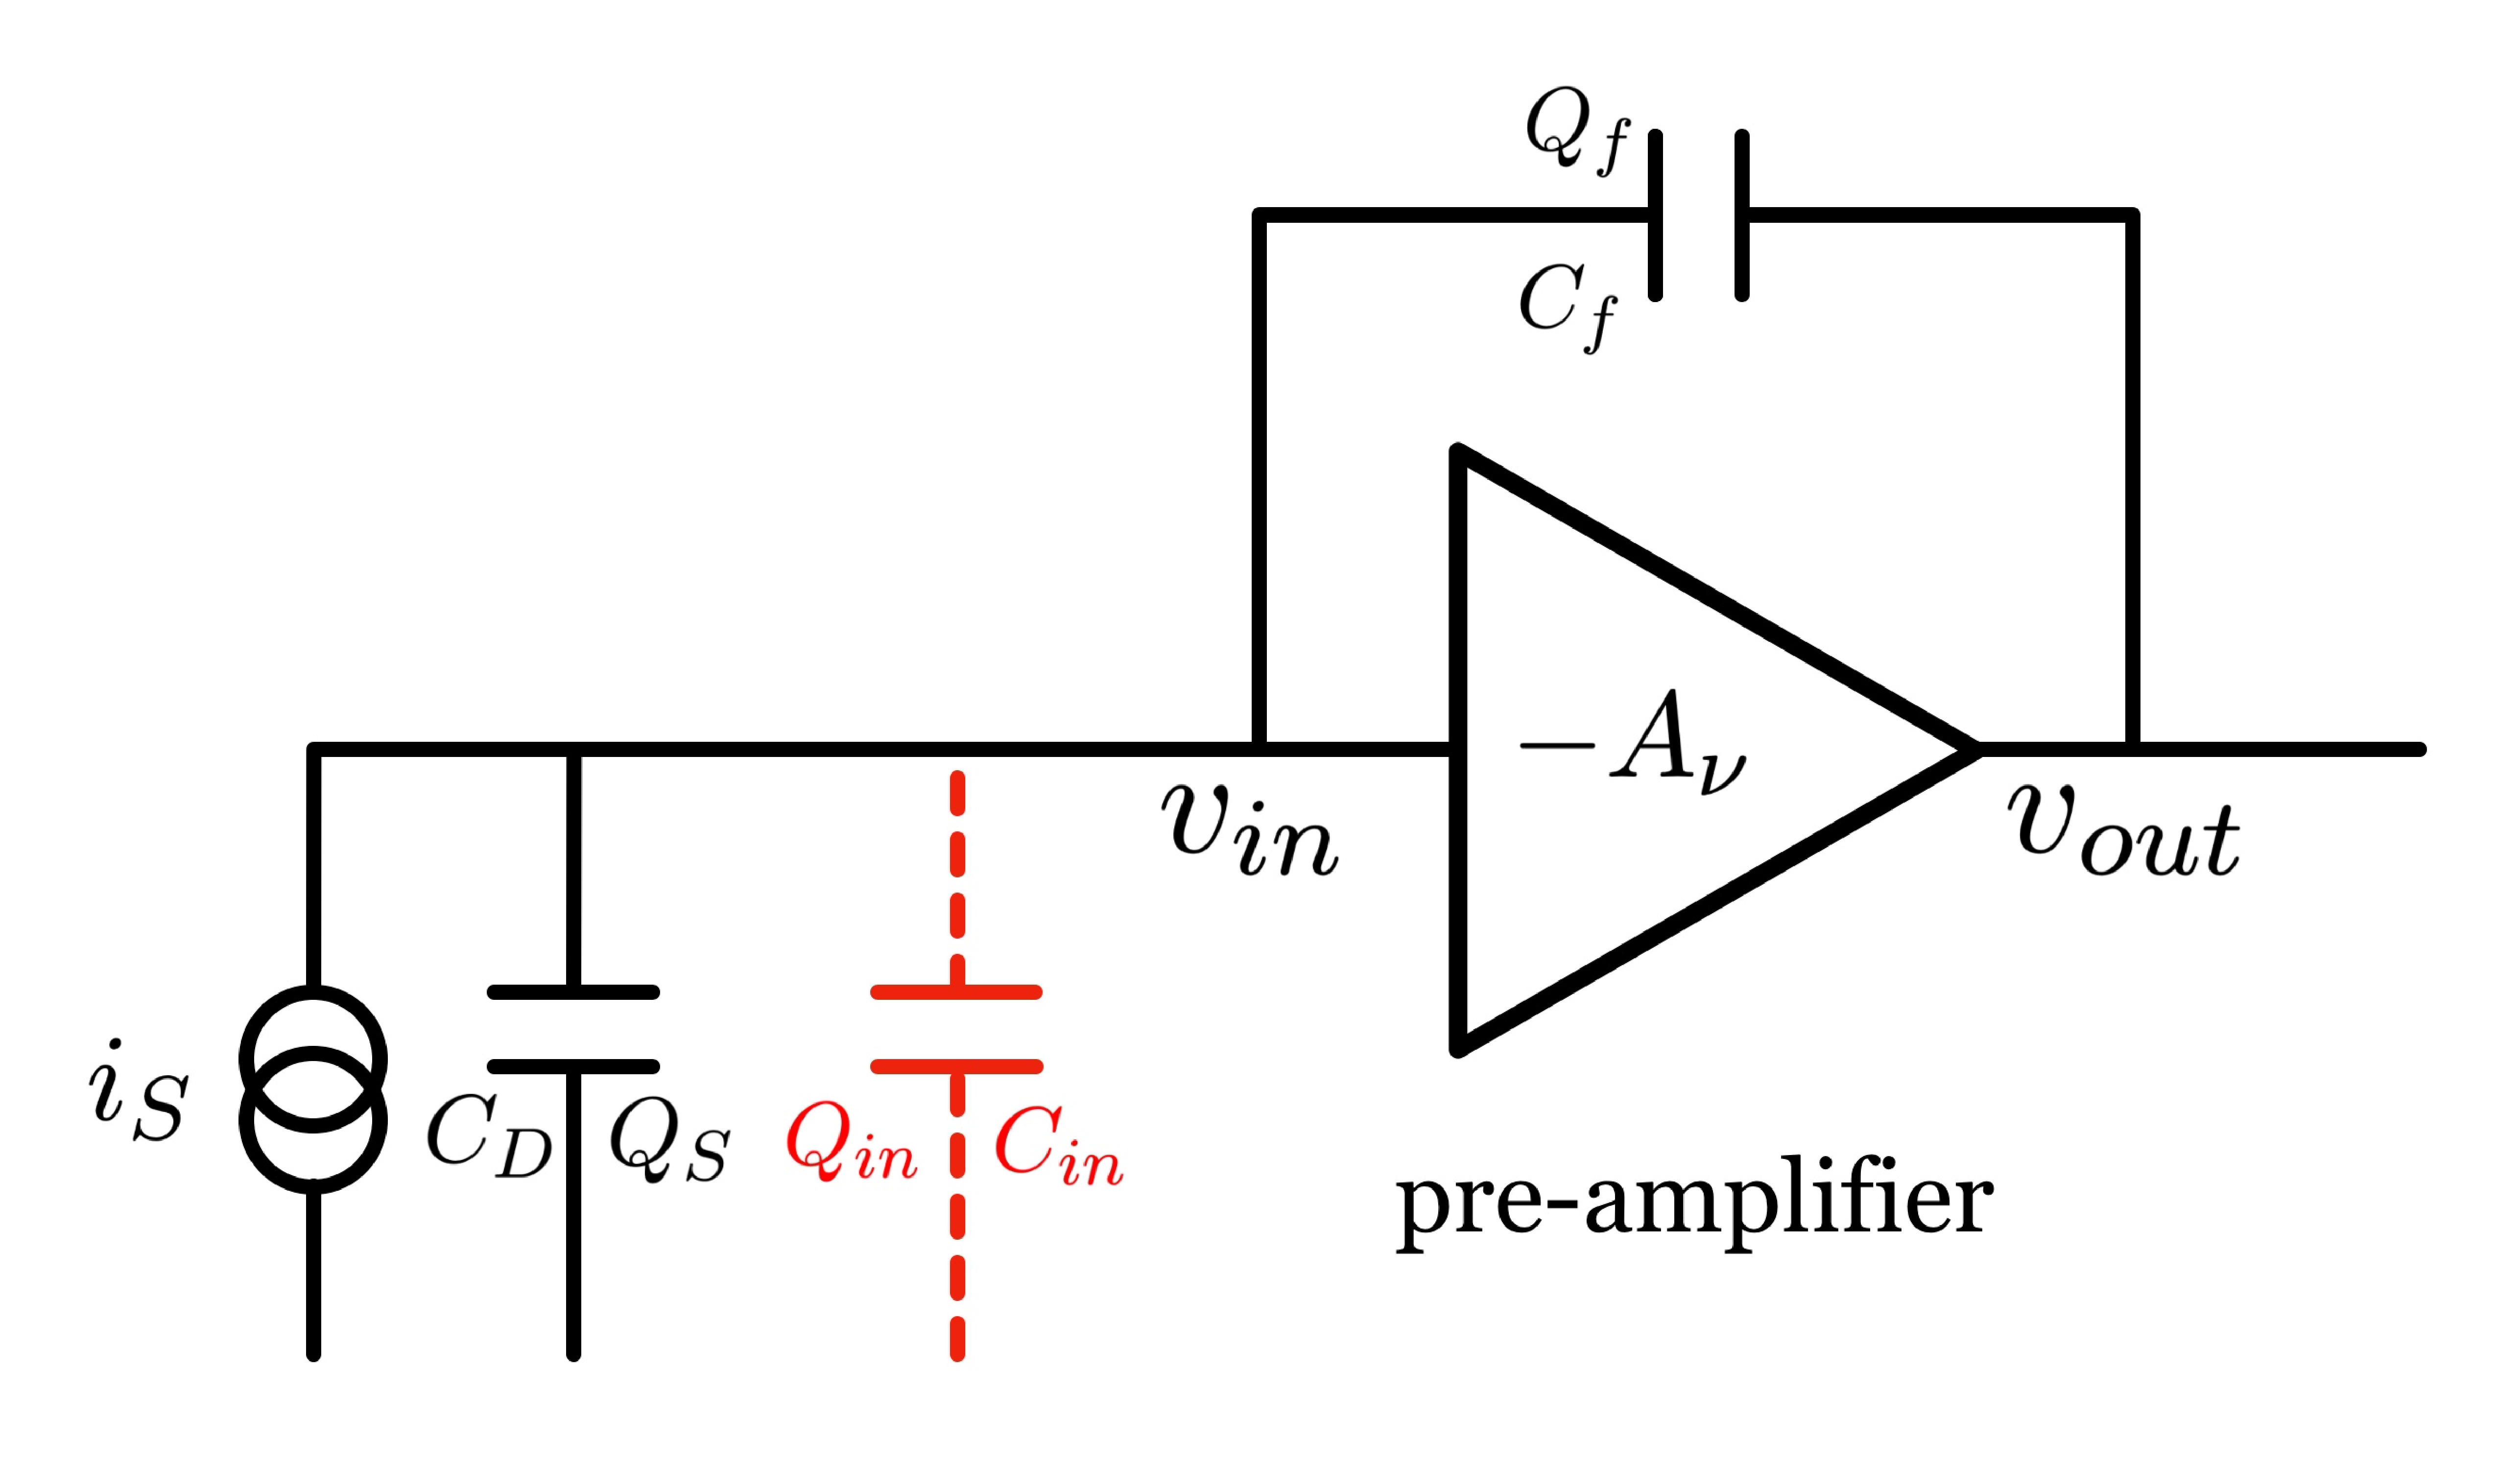
\includegraphics[width=0.9\linewidth]{files/CSA_block_diagram}
		\caption{Charge Sensitive Amplifier block diagram}
		\label{ }
		\end{minipage}
		\end{figure*} 

		The output voltage of the inverting OpAmp can be written as a function of the feedback capacity $C_f$ as follows: 
		\begin{equation}
			v_{out}(t) = -A_\nu v_{in}(t) = -\frac{1}{C_f} \int_0^t i_S(t') dt' = -\frac{Q_{in}(t)}{C_f}
		\end{equation}
		The voltage difference over the feedback capacitor is given by: 
		\begin{equation}
			v_f = v_{in} - v_{out} = v_{in}(1+A_\nu) = \frac{Q_f}{C_f}
		\end{equation}
		Since there is no current flowing into the OpAmp, the feedback charge $Q_f$ on the capacitor $C_f$ is equal to the signal charge in input to the amplifier $Q_{in}$. One can then define a dynamic input capacitance for the amplifier: 
		\begin{equation}
			C_{in} = \frac{Q_{in}}{v_{in}} = C_F(1+A_\nu)
		\end{equation}
		For sufficiently large internal gain of the OpAmp, the charge amplification can be characterised by its charge gain and reads: 
		\begin{equation}
			A_Q = \frac{v_{out}}{Q_{in}} = \frac{-A_\nu v_{in}}{(C_{in}v_{in})} \approx \frac{-A_\nu}{1+A_\nu} \frac{1}{C_f} \approx -\frac{1}{C_f}
		\end{equation}
		
		In practice, the capacitance of the detector is not negligible, and some charge remains in the detector since it is partitioned between the detector capacitance and the amplifier's feedback capacitance. The ratio between the charge in input to the amplifier and the total induced charge $Q_S$ is given by:
		\begin{equation}
			\frac{Q_{in}}{Q_S} = \frac{C_{in}}{C_{in} + C_D} = \frac{1}{1+\frac{C_D}{(1+A_\nu)C_f}}
		\end{equation}

		It is interesting so see that the gain of a CSA depends on the feedback capacitance. This is an important aspect as one can understand that if the feedback capacitance would be a free parameter of the front-end, one could act on the sensitivity to input charge desired for a (nearly) constant discrimination threshold in the discriminator. Although, for high gain of the amplifier, i.e. low feedback capacity $C_f$, if the detector capacity is significantly larger, a non-negligible part of the charge will remain in the detector. The charge gain of the amplifier can be corrected accordingly so that: 
		\begin{equation}
			A_Q = \frac{v_{out}}{Q_S} = \frac{v_{out}}{Q_{in}}\frac{Q_{in}}{Q_S} = \frac{-A_\nu}{1+A_\nu} \frac{1}{C_f} \cdot \frac{1}{1+\frac{C_D}{(1+A_\nu)C_f}} \approx - \frac{1}{C_D + \frac{C_f}{A_\nu}}
		\end{equation} 
		Even in the case, a large voltage gain $A_\nu \gg C_D/C_f$ is going to give the same result as before where the charge gain only depends on the inverse of the feedback loop capacitance. These considerations are made for an ideal case of an amplifier with infinitely large bandwidth (BW) or equivalently infinite input impedance $Z_{in}$. 

		This condition is not necessary realised for BJTs but if we denote by $R_{in}$ the input resistance of the amplifier, the above discussion holds if the following condition on the input impedance is realised:
		\begin{equation}
			Z_{in} \gg \frac{1}{2 \pi f_P C_{in}} \hspace{5mm} \Rightarrow \hspace{5mm} f_P \gg \frac{1}{2\pi Z_{in} {\left( 1 + A_\nu \right)C_f}}
		\end{equation}
		The above equation show the condition under which the transfer function of the amplifier becomes that of a typical integration circuit. For the BJT this translates to the fact that the impedance associated to the feedback capacity $C_f$ is small enough compared to $R_{in}$ so that all the current flows to the feedback loop made by the feedback resistance and the capacitance between the base and the collector of the BJT. Unless the amplifier is operated at frequencies higher than the first pole of the amplifier, in a region where the ratio between input and output exhibit a - \SI{20}{\decibel}/decade slope, it won't behave as a CSA. The finite BW will also put a constraint on how fast the output voltage can rise but will also provide more stability to the amplifier as it means operating it at lower gain. A comparison between ideal and realistic response in the frequency and time domain are presented in the figure below:  
		
		\begin{figure}[h]
		\centering
		
\includegraphics[width=0.9\linewidth]{files/CSA_transfer_function}
		\caption{Transfer function of a Charge Sensitive Amplifier}
		\label{ }
		\end{figure}
		\note{Put the diagram with impedance and not $A_v$ on the axis vertical axis}
		\note{Should I insert a schematic view of the front end with the BJT ?}\\
		In the ideal case of a CSA discussed previously, theew is no resistor in the feedback loop but only the feedback capacitor, this leads to an output level constantly increasing with time for every signal inputed in the amplifier. The addition of the feedback resistance plays a role in discharging with exponential characteristics the feedback capacitance in the feedback loop with a time constant given by $\tau_{discharge} \simeq R_f {\left( C_{det} + C_f (1+A_\nu) \right)}$ \note{add value for our BJT}. The discharge time is an essential parameter of the front-end electronics as it also contributes in defining was is the maximal rate at which the detector can be operated. The same resistance is also essential for controlling what is the voltage gain of the amplifier as it controls how much current from the output is re-injected in the input. As seen in \note{insert figure ref}, since the amplifier inverts the input signal, by reducing the feedback resistance, the voltage gain is reduced as more signal of opposite polarity is injected in the input.
		
		
		\subsection{Equivalent Noise Charge}\label{subsec:2.3.3}
		Since there exist no perfectly accurate measurement system, the characterisation of the noise contribution to the total signal noise is essential in defining both the timing performance and the energy or charge sensitivity of a detector coupled to a readout system. The influence on the noise on the signal from the detector is mainly associated in semiconductors to Landau fluctuations in the charge deposition across the detector's thickness as well as recombination of electron hole pairs. Fortunately, the contribution to the noise from the detector is negligible in contrast to the electronic noise \cite{detectors}. Recalling that a detector readout system implements a discriminator stage comparing the output of the amplifier to a threshold voltage, it becomes clear that the lower the voltage noise and the more sensitive the detector will be to small energy deposition. Concerning the timing performance of the detector system, the time resolution $\sigma_t$ has various contributions both from different aspects of the front-end discussed later (\note{cite the section}) but is often limited by the time jitter ($\sigma_{jitter}$) defined as follows: 
		\begin{equation}
			\sigma_{jitter} = \frac{\sigma_V}{\frac{dV}{dt}}\simeq  \frac{t_{rise}}{SNR} = \frac{\sigma_V}{A_q} \frac{t_{rise}}{Q_{in}} \hspace{4mm} \rightarrow \hspace{4mm} \sigma_{jitter} = \frac{ENC}{i_{S}}
			\label{eq:time_jitter}
		\end{equation}
		where we have introduced $\sigma_V$ as the voltage noise on the signal, $dV/dt$ the signal's slope, $t_{rise}$ the rise time of the signal and $SNR$ the Signal to Noise Ratio of the front-end defined as the ratio of input charge scale to the charge gained by the signal's voltage noise. The last step in equation \eqref{eq:time_jitter} introduced the concept of Equivalent Noise Charge (ENC) and represents the input charge in electrons that would need to be fed to the input of the amplifier in order to produce an output voltage equivalent $\sigma_V$. Noise is usually the consequence of fluctuations, in this case of charge carrier densities $N$ or velocities $v$ so that the fluctuation on a current flowing between two electrodes separated by a distance $d$ can be expressed as: 
		\begin{equation}
			i = \frac{Nev}{d} \hspace{5mm} \rightarrow \hspace{5mm} \sigma_i^2 = {\left( \frac{ev}{d} \sigma_N \right)}^2 + {\left( \frac{eN}{d} \sigma_v \right)}^2
		\end{equation}
		Three different noise sources can be identified: the thermal noise associated to the thermal fluctuation in velocities of charge carriers, the shot noise and $1/f$ noise which are collectively associated to the variation in number density of charge carriers \cite{detectors}.
		For a BJT, two separate equivalent noise sources can be identified that are the parallel and series noise sources. The first noise source accounts for thermal noise in the base resistance of the BJT and shot noise in the collector while the more significant parallel noise accounts for shot noise produced by the leakage current in the base. The contribution to the ENC from the amplifier can be qualitatively expressed as a function of the shaping time $\tau_m$ such that:    
		\begin{equation}
  			ENC(\tau_m) = \sqrt{2 \frac{a}{\tau_m} {\left( C_{det} + C_{in} \right)}^2 + 4 \frac{\ln(2)}{\pi} b{\left( C_{det} + C_{in} \right)}^2 + \frac{2}{3}c \tau_m} 
		\end{equation}
		where $a$, $b$ and$c$ respectively accounts for the series white noise sources, $1/f$ noise which is usually negligible for BJTs \cite{Paolozzi_thesis} and parallel white noise sources. This expression shows that for integration of fast signals, the contribution of the BJT to the ENC will be dominated by the series noise while at higher integration times ( \SI{1}{\micro\second} and above), the parallel noise takes over and the leakage current of the base of the transistors deteriorates its desired low noise performance. Looking more in detail into the series noise of the BJT, it can be qualitatively expressed as a function of the base resistance $R_b$ and the current gain $\beta$ and reads \cite{Paolozzi_thesis}: 
		\begin{equation}
  			ENC_{series \hspace{1mm} noise} \propto \sqrt{k_1 \frac{{\left( C_{det} + C_{in} \right)}^2}{\beta} + k_2 R_b {\left( C_{det} + C_{in} \right)}^2}
  			\label{eq:ENC_series}
		\end{equation}
		where $k_1$ and $k_2$ are constants. The above equation shows that in order to further mitigate the contribution of the series noise in a BJT, one would need to have a reduced the base resistance $R_b$ and also profit from a high current gain $\beta$. Moreover, it is interesting to note that this noise also depends on the detector capacitance. Therefore, minimising the noise of the amplifier is also accomplished through the minimisation of the detector capacitance.

		
		\subsection{SiGe BiCMOS HBTs}\label{subsec:2.3.4}
		
		The SiGe BiCMOS technology implements into standard CMOS nodes a SiGe HBT and is used in diverse field where low noise and very fast amplifiers are required. In regular silicon BJTs amplifiers, the transport mechanism of charges in the base is governed by diffusion which is a relatively slow and inefficient process due to its isotropic nature. A faster and much more efficient transport mechanism is drift, which requires the presence of an electric field driving the movement of charges toward the collector. The introduction of an epitaxially grown SiGe film in the base of the transistor with a linearly graded Germanium profile produces the band structure as follows. 
		\begin{figure}[h]
		\centering
		\includegraphics[width=0.9\linewidth]{files/SiGeBand_Structure}
		\caption{Band structure of a BJT (dashed line) in comparison to the ones of a SiGe HBT (solid line) \cite{SiGEHBT_band_Structure}}
		\label{im:SiGe_bandstructure}
		\end{figure}
		
		The band structure of such a device effectively implements an electric field driving the drift mechanism of electrons from the base of the transistor into the collector. The net effect is an increased current gain $\beta$ resulting in an improved transition frequency $f_T$. A secondary benefit of the SiGe HBTs comes from the directionality of the transport mechanism. In standard BJT, in order to maximise charge injection efficiency, a large collector-base surface contact is needed but this is no longer the case for SiGe HBTs. The size of the collector-base contact can be reduced hence reducing the collector base capacitance $C_{BC}$. As discussed in section \subsecref{subsec:2.3.2}, the gain of the amplifier is proportional to the inverse of the capacitance in the feedback loop which is for the BJT the collector-base capacitance, this effect also lead to a much higher charge amplification. Finally the smaller size of the base also reduces its resistance $R_b$ giving the SiGe HBTs, along with the high current gain $\beta$, the two key features required to minimise the ENC of the BJT and enhance its low noise performances.
		
		The 130nm SiGe BiCMOS HBT node from IHP (SG13G2) can reach a cut-off frequency of $f_T = $ \SI{350}{ \giga\hertz} when alimented with the nominal bias, for this reason and all the advantages discussed previously, this technology was used in the different ASICs studied in this work, It is important to specify that SiGe HBTs were implemented only in the regions requiring high analog performance where as the rest of the design (98\%) used standard CMOS technology \cite{Picardi_thesis}. When operating such amplifiers, what defines the working point of the device is the desired gain in a range of operating frequencies. By increasing the bias given to the amplifier, the cut-off frequency increases, increasing at fixed gain the bandwidth and allowing a higher operation frequency. On the contrary if the power consumption of the device is a constraint, reducing the bias given to the amplifier with reduce its bandwidth. 
		
		Throughout this work, both type of operations will be discussed, for very different applications. The MONOLITH project aims at developing an ASIC for ultra fast timing and so will require operating the transistor in the high transition frequency regime as discussed in \note{insert ref to section about monolith ASICs} whereas the ASIC designed for FASER has stricter requirements on power consumption than timing performance which will be discussed in details in \note{insert reference to section discussing FASER ASIC requirements}.   
		
		
		\clearpage

	\section{Pixelated detector technologies }\label{sec:2.4}
	
	Semiconductor devices in High Energy Physics (HEP) are usually arranged in two different geometries. Strip detectors which consist of long and fine collection electrodes with a pitch in the range of \SI{50}{\micro\meter} to \SI{100}{\micro\meter}. Pixelated detectors implementation, which we will focus on throughout this discussion, are subdivided in multiple sensitive areas arranged in a periodic pattern, like an additional subdivision of the strip. The pixel defines the smallest sensing unit in the detector and the position information of the passage of the particle is associated to the position of the pixel in the detector. If we define as $p$ the pitch on a specific direction of the pixelated detector (as pixel do not necessarily have a the same pitch in every space dimension), and $\rho(x)$ the probability density function, the resolution on the hit position of the particle is defined as follows: 
	\begin{equation}
		\sigma_x^2 = \int_{-p/2}^{p/2} x^2 \rho(x) dx = \frac{1}{12} p^2 \hspace{4mm} \rightarrow \hspace{4mm} \sigma_x = \frac{1}{\sqrt{12}} p
		\label{eq:spatial_resolution}
	\end{equation} 
	The above equation is valid for squared and rectangular pixels, for more specific geometries like hexagonal pixels used in this work, one need to build the probability density function along one of the axis used for the reference system using hexagonal pixel and compute the integral as in \eqref{eq:spatial_resolution} and would obtain $\sigma = \sqrt{\frac{5}{24}}p$. The resolution is the same along any axis of the hexagon. \\ \note{cite Matteo's Thesis}

	When an electronic readout systems needs to be coupled to the active part of the detector, two approaches are usually considered: 
	\begin{itemize}
		\item Hybrid detectors, for which the sensitive part of the detector and the readout system are implemented in two different dies and are later interconnected during the assemble procedure,
		\item Monolithic detectors, implementing directly within the same silicon die, both the sensitive part and the readout electronics. 
	\end{itemize}
		Both implementation technologies have advantages and limitations and a non exhaustive comparison between the two will be presented in the following subsections. 
	
		\subsection{Hybrid pixel detectors }\label{subsec:2.4.1}
	
		Hybrid pixelated detectors are assembled devices where the active chip is manufactured is a sensor grade silicon substrate while the readout chip is manufactured in a different silicon substrate more suited for the integration of readout electronics. Both chips have a pixelated electrode structure and are required to have a precise match between the two chips for both pixel pitch and electrode size so that each pixel on the sensitive chip has a one to one geometrical correspondence to a pixel on the readout chip.
		
		\note{could substitute sensitive chip with active and readout chip with passive}
		The connection between the two electrode on each chips is realised with a conducting micro-connection also called bump bond, which consists in the creation through diverse techniques of a soldering metallic ball directly on top of the electrodes of the readout chip \cite{flipChip}. The two chips are then put together using state of the art flip-chip techniques, precisely aligning the two dies and soldering the electrodes together through the soldering ball. Historically, bump bonding techniques were considered as a bottleneck for achieving high pixel density devices with typical sizes of \SI{150}{\micro\meter} \cite{flipChip}. Thanks to the technical improvements in the bump deposition process, the connection can now be relatively short, usually in the range of \SI{10}{\micro\meter} to \SI{20}{\micro\meter} allowing for very dense designs and mitigating unwanted parasitic effects. 
		
		\begin{figure}[h]
			\centering
			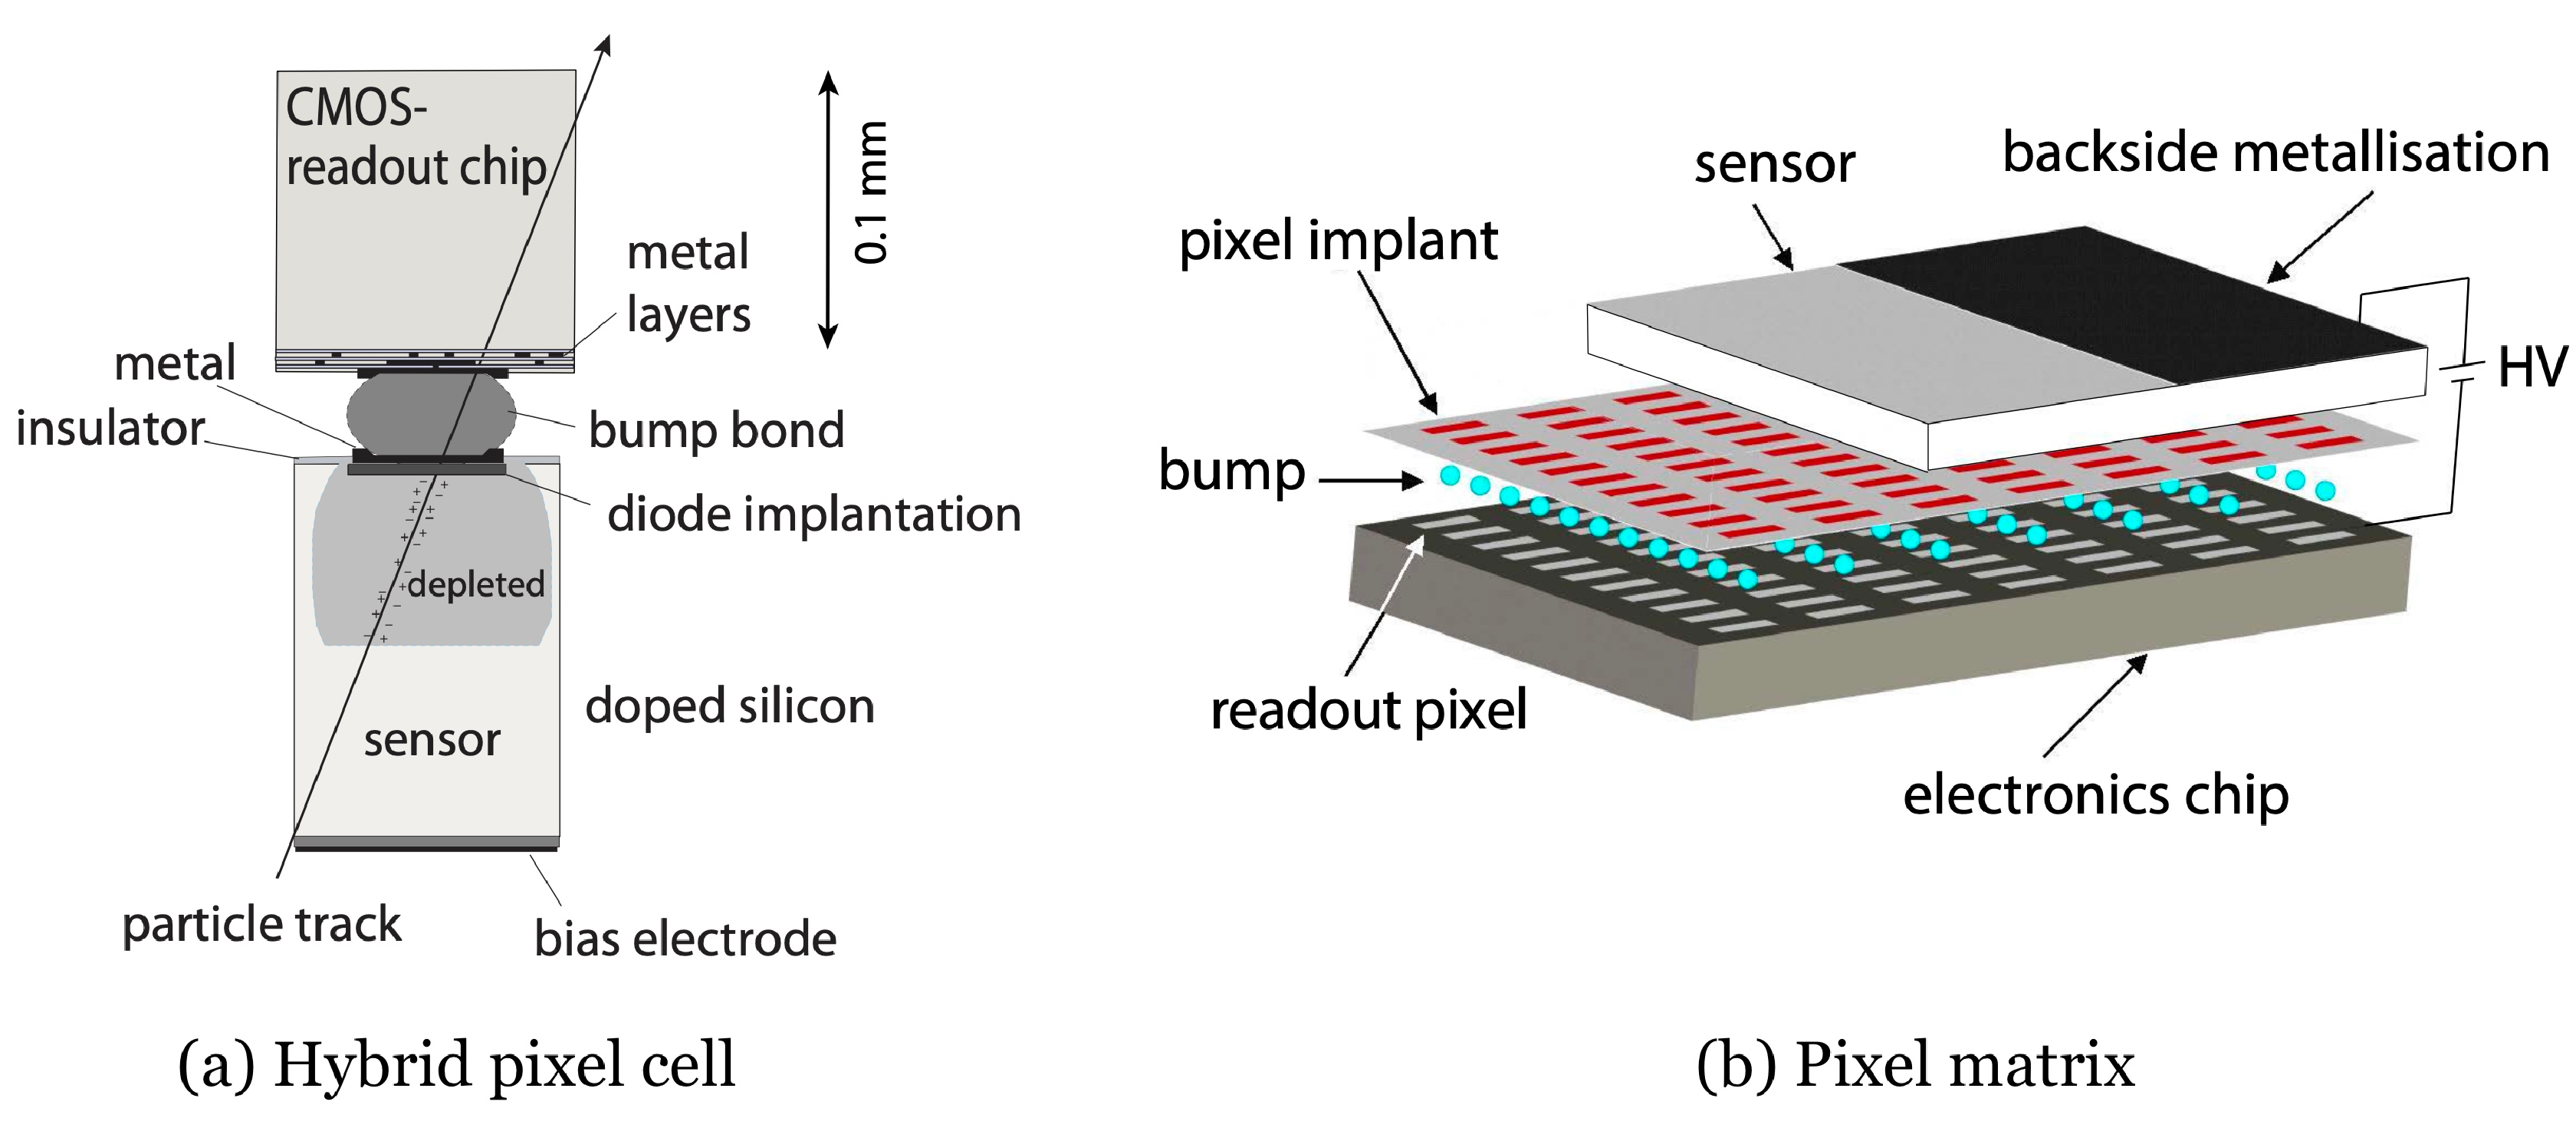
\includegraphics[width=0.9\linewidth]{files/hybrid_detector}
			\caption{Hybrid pixel detector: (a) layout of an individual pixel cell with both active (bottom) and passive (top) parts and (b) matrix of pixels showing the pixelisation of both the active sensor and readout electronics sensor, interconnected through bump-bonding \cite{detectors}}
			\label{ }
		\end{figure}
		
		 The sensitive chip often consists in pixels of \SI{50}{\micro\meter} pitch to enhance spatial resolution and have a sensor thickness typically in the range of \SI{300}{\micro\meter}. The capacitance of these devices is usually in the range of \SI{100}{\femto\farad}, mostly affected by the neighbouring pixels rather than the backside due to their thickness. As mentioned before, the detector capacitance plays a key role in defining the performance of the sensor once coupled to readout electronics. Typical hybrid sensors provide timing performances in the order of \SI{10}{\nano\second} and their low noise and low power consumption has made them suitable candidates for many HEP applications \cite{Picardi_thesis}. 
		 Many LHC experiments have chosen hybrid devices to build the inner-most tracker of their detector \cite{pixel_vertex_detector}. This region being very close to the collision point, it is exposed to a very harsh radiation environment with fluencies reaching after 10 years of operation levels of $10^{15} $ 1 MeV neutron equivalent/ cm$^2$. The detectors chosen for these inner trackers implement planar silicon sensors for the sensitive chip and have proven to be radiation tolerant and remain operable in their operation time scales. 
		 
		 The architecture of hybrid pixelated detectors makes possible a separate but parallel development and improvment of the sensitive and the readout chip in order to achieve better performances. For applications concerned with fast timing performances, readout chips like the TimePix4 \cite{timepix4} ASIC have already demonstrated a time resolution of \SI{60}{\pico\second} and some more ambitious projects like PicoPix \cite{picoPix} aims at a time resolution of \SI{10}{\pico\second}. This time resolution is only a constituent of the bigger picture where the intrinsic time resolution of the sensitive chip needs to be accounted for too. Nowadays the most promising technologies are 3D trenches silicon sensors for reduced charge collection time and planar silicon sensors with gain layer for internal charge amplification and reduced electronic noise.  \\
		 
		 Hybrid pixelated detectors have demonstrated their ability in providing a solution in terms of detector compactness, spatial and timing resolution needed for the very constrained and highly performance-demanding region that is the one closest to the interaction point in HEP experiments. Nevertheless this detector technology still present as of today some limitations like their complex and expensive manufacturing and assembly procedure. The material cost is improved in contrast to older detector technologies but the need for a sensitive chip, readout chip, support and cooling still constitutes a restrain for further improvements in overall detector performance. 
		  
		
		\subsection{Monolithic pixel detectors }\label{subsec:2.4.2}
		
		Pixel detectors made their way to particle physics experiments in the beginning of 1990 and soon started to fill the detectors of the LHC experiments. In parallel to the development of hybrid pixelated detectors, some efforts were made to develop monolithic, but were first discarded as the progress made in performance with hybrid implementation made them suitable candidates for various applications \cite{pixel_wheredowestand}. After a bit of time, improvements in the maximum resistivity of the substrate for the operation of the electronics but also in the size of the transistors used in the electronics themselves made monolithic pixel detectors more attractive. They indeed not only reached the level of performance required to make them attractive for LHC experiments but also put forward compelling advantages with respect to hybrid implementation. \\
		
		Monolithic pixelated detectors have both the sensitive part of the detector and its readout electronics included in the same substrate making it a single entity. This unlocked the potential to produce a full detector system using standard CMOS process \cite{Picardi_thesis}. 
		
		The first advantage of a monolithic implementation has already been put under light: the complex and costly assembly process of hybrid detectors is no longer an issue and allows the production of low-cost and large volumes together brought up by the use of CMOS technology. For LHC experiments applications, the material cost is an essential factor as it influences the resolution on the reconstructed track associated to a particle, more material increases multiple scattering and reduces the resolution. For the ATLAS and CMS experiments, the hybrid pixel detector represent a material thickness in excess of 3$\%$ of a radiation length per detector layer \cite{detectors}. The active sensor and passive readout electronics being in a the same substrate for monolithic pixel detectors, the material cost could be reduced up to a factor of magnitude if the detector can be build on a self-supporting structure and operated with low enough power densities to minimise the need for cooling \cite{detectors}. The requirements on monolithic pixel detectors also include a sufficiently large signal-to-noise ratio to allow for a low noise operation together with a good radiation tolerance against ionising and non-ionising radiation (for more details on radiation tolerance see \note{cite section}). 
		
		The ability to use the full CMOS technology, meaning both NMOS and PMOS transistor on the same substrate is essential to unlock the true potential of CMOS logic in monolithic detectors. Initially monolithic sensors were made using a low resistivity p-type substrate on which an epitaxial Silicon layer was grown with higher resistivity than the substrate and freedom in the choice of type. A schematic view of such a sensor is given in the figure below: 
		\begin{figure}[h]
			\centering
			\includegraphics[width=0.9\linewidth]{files/MAPS_noHV}
			\caption{Cross section view of a typical monolithic sensor implementation without external bias voltage for depletion and including both PMOS and NMOS transistors.}
			\label{im:initial_mono_XS}
		\end{figure}
		
		 The thickness of the epi-layer depends on the applications and is usually in the 1-\SI{20}{\micro\meter} range, the electronics are then implanted at the top of the epi-layer. When particles cross the epi-layer, charge can be deposited both in the small depleted region below the collection electrode and mainly in the non depleted epi-layer. The collection of charge from the depleted region will be fast and complete thanks to the drift of charges carriers whereas the collection from charges from the non depleted epi-layer will be driven by diffusion and hence be incomplete and comparatively slow ($>$ \SI{100}{\nano\second}) \cite{detectors}. The collection electrode is in this case a n-type well and the use of NMOS transistors laying in a p-type well is not problematic whereas the use of PMOS transistors laying in a n-type well would constitute a competing electrode for charge collection. For this reason, n-type well for electronics have to be shielded by a deep highly doped p-type well implanted below the n-type well in the epi-layer. 
		 
		 This design offers as an advantage a reduced total thickness (in contrat to hybrid detectors) in the range of 50-\SI{150}{\micro\meter} \cite{detectors} and hence a reduced material cost per layer  if implemented in an experiment. The down-side is the time resolution of such devices, which would only be suitable for experiments such as the ALICE detector for heavy ions collisions \cite{alpide}. In order to obtain a much faster and complete charge collection to satisfy requirements or other LHC experiments, it is straightforward that monolithic sensors have to be fully depleted to have a drift-driven charge transport in the active part of the sensor. As seen in equation \eqref{eq:depletion_width}, the depletion thickness can be written such as: 
		 \begin{equation}
		 	d_{depletion} \approx \sqrt{V \rho}
		 \end{equation}
		
		This implies that the choice of process technologies employed must allow higher voltages than the ones usually required by standard CMOS technologies \cite{peric} or be able to process high resistivity wafers, or a combination of both \cite{detectors}. The chosen technology also needs to provide multiple wells both for shielding and implementation and NMOS and PMOS transistors. Two different approches in realising such detectors have been considered: the small collection electrode and large collection electrode design which we will now discuss.
		
		\subsubsection{Small Collection Electrode}
		The small electrode configuration has a n-type well separated from the CMOS electronics, due to its shrunk size it allows for a small collection node capacitance in the range of 5-\SI{20}{\micro\meter} \cite{detectors} which is of concern for noise and timing performances as seen in \eqref{eq:ENC_series} and \eqref{eq:time_jitter}. This implementation is also not optimal in terms of radiation tolerance as trapping probability of defects in the lattice (see more in \note{cite section on rad tolerance}) is linked to the collection time and is usually longer for small electrodes as the electric field is not uniform across the region separating two electrodes. The figure below gives a generalised schematic view of the small collection electrode implementation: 
		\begin{figure}[h]
			\centering
			\includegraphics[width=0.9\linewidth]{files/MAPS_small_electrode}
			\caption{Schematic cross section of the small electrode implementation for monolithic pixel sensors. An additional n-type layer is added to ease the full depletion of the sensor.}
			\label{im:small_electrode}
		\end{figure}
		
		Achieving full depletion in small electrodes designs is not straightforward and a modification of the process involving the addition of a low dose n-type implant below the pixel is required \cite{thanu_small_electrode}. This modification has the overall effect of strengthening the electric field laterally and so improve charge collection laterally too. The small charge signal created in the thin epi-layer (typically in the range of 1600 $e^-$)\cite{detectors} is not too much of a constraint as the collection node capacitance is small and since the voltage is given by $dv = dQ/C_D$, resulting in a voltage difference in the range of \SI{50}{\milli\volt}, a voltage amplification stage is hence usually used. 
		For small electrodes design, a small pixel size is usually preferred to mitigate the negative effect on radiation tolerance and timing performance, this comes at the cost of a higher required power density as the power consumption is roughly constant per pixel. 
		
		
		\subsubsection{Large Collection Electrode}
		The alternative is a large collection electrodes for the implementation of monolithic pixels detectors. This means that the collection electrodes covers most of the area of the pixel, this leads to a set of advantages but also limitations in contrast to the small collection electrode. The figure below presents a generalised schematic view of the large collection electrode implementation. 
		\begin{figure}[h]
			\centering
			\includegraphics[width=0.9\linewidth]{files/MAPS_large_electrode}
			\caption{Schematic cross section of the large collection electrode implementation for monolithic pixel detectors.}
			\label{im:large_collection_electrode}
		\end{figure} 
		
		In this configuration, full depletion is achieved from the top surface or from the backside through the realisation of a backside processing allowing for a backside contact for depletion voltage.
		Having a much more uniform weighting field, the collection of charges is more uniform and also faster as the collection path is shorter than for small collection electrodes. This benefits to the radiation tolerance of the sensors since the trapping probability will be reduced, but also to the timing performance. On the contrary, the large collection electrodes, together with the implementation of close-by deep n-type and p-type wells, presents to the input of the amplifier a large detector capacitance (in the range of several hundreds of \SI{}{\femto\farad}), having a negative impact on both noise and timing performances. An optimisation of both electrode geometry and internal junctions is essential to a reach the best performances of the sensor for a fixed power consumption \cite{Picardi_thesis}. \\
		
		Many different pixel designs have been realised in both configurations, showing a high rate capability and radiation tolerance to comply with the level required at the LHC \cite{detectors}. Throughout this work, monolithic pixel detectors with large collection electrodes will be presented. This work will not focus on the design of such devices but rather on the extensive qualification and understanding of their features, both for the development of the FASER Pre-Shower but also for the ultra fast timing performances of concern for the MONOLITH project. 
		\clearpage

	\section{Effects of radiation \textcolor{blue}{ 4 pages}}\label{sec:2.6}
		\subsection{Processes involved \textcolor{red}{ 2 pages}}\label{subsec:2.6.1}
		\subsection{Consequences of damages and solutions \textcolor{red}{ 2 pages}}\label{subsec:2.6.2}

\clearpage

\chapter{Monolithic pixel detectors for HEP applications (30 pages)}

%Monolithic silicon pixel detectors were previously described in chapter \note{chapter ref} and their promising performances for potential upgrades of current experiments or the development of novel experiments was highlighted. Notably, in \note{chapter ref} were discussed the prospects of the installation of a new pre-shower detector for the FASER experiment using Silicon-based pixel detectors for the active part of the detector. 

At the University of Geneva, the development of silicon-based monolithic pixel detectors has been carried out since 2016. The design of the sensors also relied on the implementation of ultra fast and low noise electronics offered by the SG13G2 \SI{130}{\nano\meter} process \cite{IHP130nm} consisting in a \SI{130}{nm} SiGe BiCMOS HBT offered by Leibniz Institute of High-Performance Microelectronics (IHP). Over the course of the years, both the sensor and the electronics design were refined in order to better understand the intrinsic limits on the performances of such devices. The research was mostly focused on investigating the efficiency and timing performance of the designed prototypes with the scope of eventually developing a very fast, fully efficient, radiation hard and low power consumption sensor, as a good candidate for applications in future colliders. In parallel, profiting from the expertise acquired, a proposal for an upgraded version of the pre-shower station in the FASER experiment was initiated.

The work presented in this chapter will first give a description of the design characteristics of two prototypes, a first one designed under the ATTRACT Phase1 MonPicoAD project, also referred to as the \textit{ATTRACT} prototype and a second one designed under the MONOLITH ERC Advanced project, also referred to as the \textit{MONOLITH} prototype. The discussion will remain at surface level as the scope of this thesis was neither the design of the sensor nor the design of the electronics but rather the testing and extensive comprehension of the features exhibited by each prototype.

One of the key figures of merit of the designed sensors is their time resolution. This performance metric is affected by many sources, some of which can eventually be corrected for. In the second part of the discussion, an overview of the different contributions to the time resolution of silicon-based sensors will be presented together their sources and also possible solutions to reduce their impact. 

The characterisation of such prototypes is essential and a robust and reliable testing procedure is required. Usually, such studies are performed using a particle beam composed essentially of minimum ionising particles. In the context of this research, prototypes were tested at the CERN SPS testbeam facility. The time resolution and detection efficiency was extracted for each prototype using a dedicated experimental setup. A reconstruction of the particle tracks onto the sensors was essential to perform position sensitive measurements. The last part of the discussion in this chapter will, in a first time cover the arguments mentioned above, and in a second time present the results of the characterisation of the \textit{ATTRACT} and \textit{MONOLITH} prototypes. Additionally, the effect of radiation on the performance obtained with the \textit{MONOLITH} prototype will also be presented for a wide range of radiation levels, up to values compatibles with the innermost layers of large experiments at CERN in the HL-LHC phase.    

	\clearpage
	\section{Prototypes and design characteristics}
	In the following section, the design characteristics of the sensor and electronic parts of the two prototypes tested in this work will be presented. The first prototype will be referred to as the \textit{ATTRACT} prototype while the second one will be referred to as the \textit{MONOLITH} prototype. Some key dates together with a list of the associated literature associated to each prototype are listed below: 
	\begin{itemize}
		\item \textbf{\textit{ATTRACT}} prototype (2019): 
		\begin{itemize}
			\item Tested in laboratory in 2020-21 and at testbeam facility in 2021, results published in: \textit{"Efficiency and time resolution of monolithic silicon pixel detectors in SiGe BiCMOS technology"} by G. Iacobucci et al. in JINST in 2022 \cite{ATTRACT_proto1_50ps}. 
		\end{itemize}
		\item \textbf{\textit{MONOLITH}} prototype (2022):
		\begin{itemize}
			\item Tested in the laboratory and at testbeam facility in 2022, results published in: \textit{"20 ps time resolution with a fully-efficient monolithic silicon pixel detector without internal gain layer"} by S. Zambito et al. in JINST in 2023 \cite{MONOLITH_proto2_20ps}.
			\item Tested after irradiation in the laboratory in 2023, results published in \textit{"Radiation Tolerance of SiGe BiCMOS Monolithic Silicon Pixel Detectors without Internal Gain Layer"} by M. Milanesio et al. in JINST in 2023 \cite{MONOLITH_RadHard_lab}.
			\item Tested at testbeam facility in 2023, results published in : \textit{"Testbeam results of irradiated SiGe BiCMOS monolithic pixel detector without internal gain layer"} by T. Moretti et al. in JINST in 2024 \cite{MONOLITH_RadHard_testbeam}.
		\end{itemize} 
	\end{itemize}

		\subsection{ATTRACT prototype}
		The \textit{ATTRACT} prototype (2019) is the second prototype designed the scope of the ATTRACT Phase1 MonPicoAD project. Its predecessor was described and tested in \cite{ATTRACT_proto1, ATTRACT_proto1_50ps}. The ASIC was manufactured by the IHP Microelectronics foundry using the IHP SG13G2 \SI{130}{\nano\meter} BiCMOS technology. The design of the ASIC was finalised in 2019 and the wafers received after post processing in 2019. The ASIC has a total size of $2.3 \times 2.5$ mm$^2$ active pixel matrix is subdivided in 12 rows and columns for a total of 144 hexagonal pixels with a \SI{65}{\micro\meter} side resulting in a pixel pitch of roughly \SI{110}{\micro\meter}. The ASIC periphery is located beside the pixel matrix and includes a Slow-Control (SC) interface through which the different bias supplied to the electronics can be controlled. The periphery and pixel matrix is then insulated from the substrate by a total of 18 guard rings which insulates the pixel well from the substrate. The pixel matrix is further subdivided into four 6x6 matrices, each containing a different design for the preamplifier part of the front-end electronics.  
			
		Within one of the four sub-matrices, a set of four pixels are connected to a SiGe HBT amplifier, used as a charge sensitive amplifier, and analog driver directly connect to the output pads. The driver itself is composed of two consecutive HBTs in common collector configuration with a first AC stage coupled to the output of the amplifier \cite{ATTRACT_proto1_testbeam}. The front-ends are located outside of the pixel well and are used to measure and amplify the charge deposited by particles in the sensor. In the results later presented in \note{insert section}, the performances quoted are referred to these four analog pixels. The remaining 140 pixels have their front-end located in pixel and are connected to a digital readout with many discrimination stages, different from one sub-matrix to the other. These pixels also have the output of their discriminator connected to a FAST-OR to provide a discriminated signal for all of them in output. 
		
		The active part of the ASIC is build as a \textit{n-on-p} sensor meaning that the pixel well is n-type and the substrate is p-type. The base substrate is doped with Boron and a resistivity of \SI{50}{\ohm \centi\meter}. After implementation, the substrate was thinned to reach a sensor thickness of roughly \SI{60}{\micro\meter}. The total pixel capacitance in input to the preamplifier is estimated to be \SI{80}{\femto\farad} with a depletion depth estimated to be \SI{23}{\micro\meter}. 
		
		An image of the prototype taken under a microscope with overlayed blocks representing the diverse sections of the ASIC is presented in figure \ref{im:ATTRACT_ASIC_layout}.
		\begin{figure}[h]
			\centering
			\includegraphics[width=0.65\linewidth]{files/ATTRACT_ASIC_layout}
			\caption{Image of the \textit{ATTRACT} prototype taken with a microscope. On top of the image are placed different block representing the different key structure in the ASIC. \note{Add zoom on pixel matrix and add analog Front-End label and names of pixels}}
			\label{im:ATTRACT_ASIC_layout}
		\end{figure} 
		
		
		
		
		\subsection{MONOLITH prototype }
		
		The \textit{MONOLITH} prototype (2022) is the second prototype of the generation of sensors without internal gain layer designed in the scope of the MONOLITH project. The ASIC was manufactured by the IHP Microelectronics foundry using the IHP SG13G2 \SI{130}{\nano\meter} BiCMOS technology. The design of the ASIC was finalised in 2021 and the wafers received after post processing in 2022. The ASIC has a (smaller) total size of $2.0 \times 2.5$ mm$^2$ active pixel matrix is subdivided in the same was as the \textit{ATTRACT} prototype. The architecture of this prototype is mostly similar to the one presented for the \textit{ATTRACT} prototype except for a few changes.  
		
		The front-end design in this prototype is different than the one implemented in the \textit{ATTRACT} prototype as it includes improvements. The first noticeable difference is in the power distribution, indeed the previously the alimentation of the preamplifier and the driver were put together but are now separated. This design change has the objective of removing undesired cross-talk between the four analog pixels. The second modification affects the stability of the front end when operated in high gain configurations. This was achieved by equipping the driver stage with a semi-differential analog output, effectively reducing the common-mode noise outside the ASIC. In addition, the new driver design reduced the signal rise-time, a key parameter in the contribution to the time resolution. Finally, in contrast to the single-ended output used previously, this prototype provides a differential output, helping by offering means to reduce the external noise contributions when analysing the signals offline. 
		
		For what regards the sensor, the ASIC is build as a \textit{n-on-p} sensor meaning that the pixel well is n-type and the substrate is p-type. The base substrate is doped with Boron and is characterised by its very low resistivity of \SI{0.1}{\ohm \centi\meter} while the \SI{50}{\micro\meter} thick epitaxial layer grown on top is still doped with Boron but with a higher resistivity of \SI{350}{\ohm \centi\meter}. This value is to be compared with the \SI{50}{\ohm \centi\meter} of the previous prototype, leading to a larger production of initial charge in the sensor when crossed by a ionising particle. The total pixel capacitance in input to the preamplifier is estimated to be \SI{100}{\femto\farad}. 
		
		An image of the prototype taken under a microscope with overlayed blocks representing the diverse sections of the ASIC is presented in figure \ref{im:MONOLITH_ASIC_layout}.
		\begin{figure}[h]
			\centering
			\includegraphics[width=0.65\linewidth]{files/MONOLITH_ASIC_layout}
			\caption{Image of the \textit{MONOLITH} prototype taken with a microscope. On top of the image are placed different block representing the different key structure in the ASIC. \note{Add zoom on pixel matrix and add analog Front-End label and names of pixels}}
			\label{im:MONOLITH_ASIC_layout}
		\end{figure} 
		 
		
		
	\clearpage
	\section{Time resolution of silicon pixel detectors \textcolor{blue}{ 4 pages}}
	One of the main focuses of the development of silicon-based monolithic pixel detectors, first under the ATTRACT project and then under the MONOLITH project, is the achievement of very good time resolution, trying to get as close as possible to the intrinsic limits of the technologies implemented. The time resolution is defined as the error one makes when measuring the time of passage of a particle in the active part. There are multiple contributions to the time resolution of a silicon-based device, both from the sensor itself, the front-end electronics and the digital readout. The contribution from the digital readout for the studies carried out in this work is the one of the oscilloscope used to readout the 4 analog pixels as explained in \note{section ref}. 
	
	In order to better explain was time walk is, a collection of waveforms from the testbeam test of the \textit{MONOLITH} prototype was put together in figure \ref{im:waveforms_timeresolution}. There waveforms were aligned vertically with respect to each waveform's average level in the region before the signal but also horizontally using a very precise timing reference. The close-up view shows the time at which each waveforms would cross a discrimination threshold labeled $V_{th}$, also known at Time of Arrival (ToA) of the signal.
	\begin{figure}[h]
		\centering
		\includegraphics[width=0.85\linewidth]{files/waveforms_timeresolution}
		\caption{Collection fo waveforms from the \textit{MONOLITH} prototype in a testbeam with 120 GeV/c pions at CERN. The image shows time and amplitude aligned waveforms for a large range of amplitudes. The zoomed-in figure shows the time at which each waveform would cross a fixed voltage threshold ($V_{th}$), highlighting the spread of the time of arrival.}
		\label{im:waveforms_timeresolution}
	\end{figure} 
	
	If one was to build a distribution of the ToA, the shape of the distribution obtained is close to the one of a Gaussian function. The standard deviation of the fit of the ToA distribution with a Gaussian function gives the total time resolution of the system composed of the sensor, the front-end electronics and the readout system. 
	
	It is possible to group into four different categories the contributions to the time resolutions as listed by \cite{timeres_SiliconDetectors}:
	\begin{itemize}
		\item \textit{Signal creation}: The distribution of the energy deposited by the impinging particle depends on the physics of the interaction, some statistical fluctuations in the signal's induction can create irregularities in the signal, labeled $\sigma_{\text{Landau}}$. The variation on the amplitude of the signal due to smaller or larger charge deposition has a contribution too, labeled as $\sigma_{\text{time walk}}$. The first contribution is an intrinsic property of the detector defined by its geometry and operation. On the contrary, the time-walk can be correct as it will later be shown.
		\item \textit{Sensor characteristics}: The uniformity of the key components taking parts in the signal inducting such as the weighting field of drift velocities of the charge carriers can also lead to a distorsion of the signal, this contribution is labeled $\sigma_{\text{distorsion}}$.
		\item \textit{Electronics}: The noise of the amplifier is the key aspect here, its impact it more or less important depending also on the slew-rate of the amplifier, or how fast the signal can rise. This contribution is labeled $\sigma_{\text{jitter}}$
		\item \textit{Digitisation}: When the analog waveform is sampled for digitisation, the uncertainties on the measured time is associated to the TDC uncertainties and is labeled $\sigma_{\text{TDC}}$
	\end{itemize} 
	
	Each single contribution can be considered as independent from the others, assuming gaussian uncertainties, the total uncertainty of the time resolution $\sigma_t$ can be expressed as: 
	\begin{equation}
		\sigma_t^2 = \sigma_{\text{Landau}}^2 + \sigma_{\text{time walk}}^2 + \sigma_{\text{distorsion}}^2 + \sigma_{\text{jitter}}^2 + \sigma_{\text{TDC}}^2
	\end{equation}
	
	It is possible to discuss each contributions individually to better understand the origins of each contribution with the scope of understanding how the design of the full detector ca be optimised. 
	
	 	\subsection{Charge collection noise contribution}
	 	The energy lost by a charged particle when traversing a material arises primarily from electromagnetic interactions, in which the transferred energy results in ionisation or excitation of the target medium. For relativistic particles with energies well above the electron mass, the average energy loss per unit length is material-dependent and is accurately described by the Bethe formula:

		\begin{equation}
			\left\langle -\frac{dE}{dx} \right\rangle = K z^2 \frac{Z}{A} \frac{1}{\beta^2} \left[ \frac{1}{2} \ln\left( \frac{2 m_e c^2 \beta^2 \gamma^2 W_{\text{max}}}{I^2} \right) - \beta^2 - \frac{\delta(\beta \gamma)}{2} \right],
		\end{equation}

		where $K$ is a constant, $z$ is the charge of the incident particle, $Z$ and $A$ are the atomic number and mass number of the medium, $\beta$ and $\gamma$ are the relativistic parameters, $I$ is the mean excitation potential of the material, and $W_{\text{max}}$ the maximum energy transferable in a single collision.

		To better illustrate the behaviour of energy loss across a wide range of particle velocities, figure \ref{im:bethe_bloch} shows the mass stopping power (i.e. the energy loss per unit length scaled by the density of the medium) in copper as a function of $\beta \gamma$, ranging from $10^{-3}$ to $10^5$ \cite{PDG}.

		\begin{figure}[h]
			\centering
			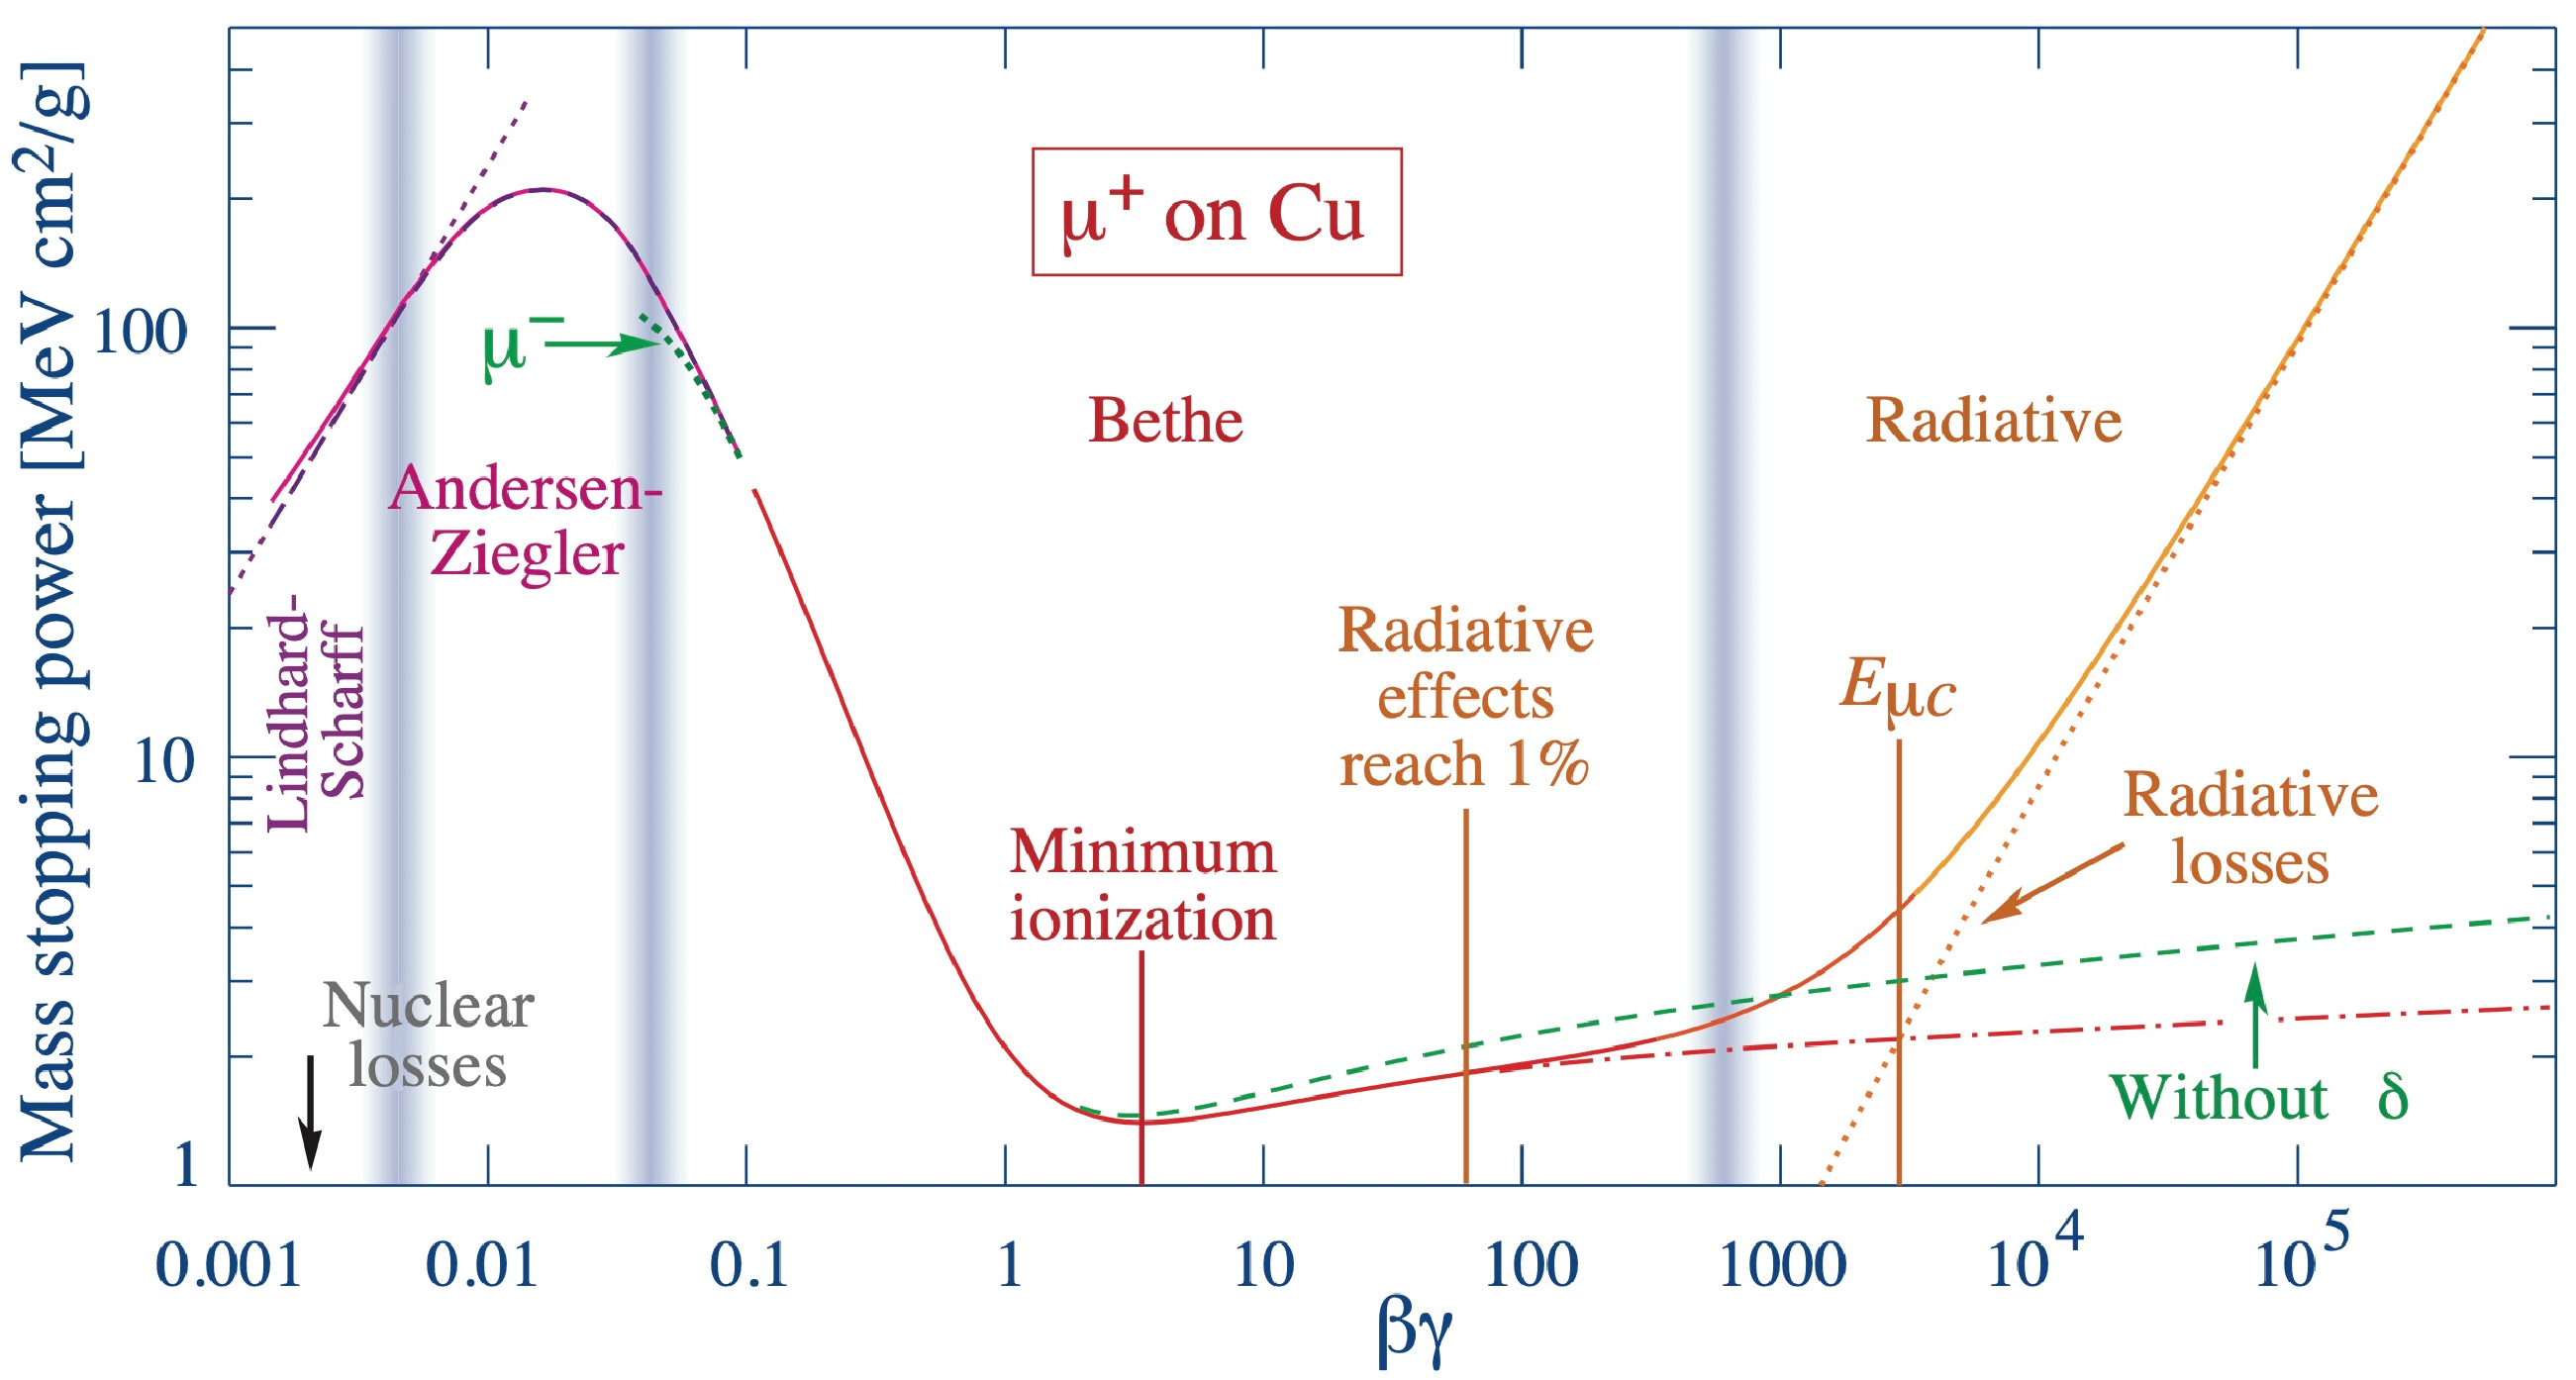
\includegraphics[width=0.85\linewidth]{files/bethe_bloch}
			\caption{Mass stopping power for charged particles with $\beta \gamma$ ranging from $10^{-3}$ to $10^5$ in copper.}
			\label{im:bethe_bloch}
		\end{figure}

		One of the key features is the minimum ionisation point, which occurs for particles with $\beta \gamma \simeq 3$. Such particles are referred to as Minimum Ionising Particles (MIPs) and exhibit the lowest energy loss due to ionisation. Beyond this point, the stopping power increases logarithmically with energy due to enhanced interactions with atomic electrons. At very high energies ($\beta \gamma \gtrsim 10^3$), radiative losses such as bremsstrahlung become dominant, particularly for light particles like electrons, while the contribution from ionisation gradually decreases.

		For electrons, radiative losses begin to dominate at energies above a few tens of MeV, leading to the production of secondary photons that can initiate electromagnetic cascades \cite{Paolozzi_thesis}. However, in the context of thin silicon detectors, these processes can often be neglected, as the mean free path of such photons typically exceeds $10\,\text{g/cm}^2$ for energies above \SI{1}{\mega\electronvolt} \cite{PDG}.

		While the Bethe equation provides the mean energy loss, the actual energy deposited by a charged particle in a thin detector fluctuates significantly due to the stochastic nature of the ionisation process. Most events result in small charge deposits well below the mean, while a few involve large energy transfers to atomic electrons , producing a long tail in the energy loss distribution. This results in a highly skewed shape known as a Landau distribution and the associated fluctuations directly impact the number of electron-hole pairs generated in the silicon and manifest as an intrinsic charge collection noise. This noise will not only create a variation in the amplitude of the signal, which is at the root of the time-walk contribution (discussed in depth later in \note{section ref}), but will also create irregularities in the induced current, also contributing to the overall time resolution \cite{timepix4}. 

		\subsection{Time jitter contribution \textcolor{red}{ 2 pages}}
		
		It was already anticipated in \note{section ref} that the different noise sources on the amplifier also contribute to the overall time resolution of the detector. These noise sources will effectively translate into an output voltage noise $\sigma_\text{V}$ onto the output voltage of the amplifier $V(t)$. The time jitter is defined as the uncertainty of the ToA due to early or late crossing of the signal to a fixed level that is the discrimination threshold $V_{\text{th}}$. The contribution of the output voltage noise on the time resolution depends on the slew rate of the output voltage signal around the level $V_{\text{th}}$ and can be expressed as
		\begin{equation}
			\sigma_{\text{jitter}} = \frac{\sigma_{\text{V}}}{dV/dt} = t_{\text{rise}} \frac{\text{Signal}}{\sigma_{\text{V}}}
		\end{equation}  
		
		where $t_{\text{rise}}$ is defined as the rise time of the signal and Signal/$\sigma_{\text{V}}$ is commonly know as the Signal-to-Noise Ratio (SNR). The slew rate can be up to a good approximation be considered as constant, this is highlighted in the zoomed-frame of figure \ref{im:waveforms_timeresolution}. The implications are straightforward, if one wants to reduce the contribution of the time jitter, the rise time of the signal must be as small as possible, and the SNR has to be as large as possible. Translating these two trends into parameters of the amplifier, this would respectively mean a large bandwidth and a large gain. Unfortunately for amplifiers there is always a trade-off between gain and bandwidth as the product of these two quantities is constant and its value is defined by the operation parameters of the amplifier itself. 
	
		Another important consideration to make is the choice of the discrimination level $V_{\text{th}}$. Indeed the slew rate of the output voltage signal is not constant over the rise of the signal. At the beginning of the rise, the slew rate progressively increases and reaches a maximum defined by the slope of the induced current and the frequency response of the amplifier. The slew rate then progressively decreases the closer it gets to the peaking time $t_{\text{peak}}$, defined as the time at which $V(t)$ reaches its maximum value, as most of the charge has been collected. As a consequence, the point with maximum slew rate is usually the time corresponding to half of the output voltage value at the peaking time. The choice of a discrimination threshold usually does not only depend purely on the time resolution considerations but this discussion is reserved for further on. 
		
		
		\subsection{Time walk contribution \textcolor{red}{ 2 pages}}
		
		
		\subsection{Other contributions \textcolor{red}{ 2 pages}}
	
	\clearpage
	\section{ Testbeam at SPS testbeam facility \textcolor{blue}{ 17 pages}}
		\subsection{Layout of test beam experiment \textcolor{red}{ 2 pages}} 
		\subsection{The FE-I4 telescope: track reconstruction \textcolor{red}{ 2 pages}}
		\subsection{Analysis methods and dataset construction \textcolor{red}{ 3 pages}}
		
%%PAPER ON ATTRACT
%\section{Efficiency and time resolution measurement}
%\label{sec:results}
%
%\subsection{Testbeam experiment setup and data set}
%\label{subsec:dataset}
%
%The detection efficiency and time resolution of the prototypes were measured at the CERN SPS testbeam facility with a pion beam with \SI{180}{\giga\electronvolt}/c momentum. The experimental setup consisted of the UniGe FEI4 telescope for particle tracking \cite{Benoit_2016}, with the two devices under test (DUT0 upstream with respect to the beam, DUT1 downstream) placed after three detection planes of the telescope as shown in Figure \ref{fig:Setup}. The DUTs were operated at room temperature. The DUTs were read by two oscilloscopes with analog bandwidth of 4 GHz and a sampling rate of 40 GS/s and 20 GS/s, respectively. The DUTs were positioned specularly to each other and pixels OA0 (shown in Figure~\ref{fig:analog_pixels}) from the two chips were aligned and sent to the oscilloscope with the largest sampling rate to make Time-Of-Flight (TOF) measurements. The data from pixels OA1 and OA2 of the two DUTs, which were not aligned among the two DUTs, were also acquired.
%
%\begin{figure}[!htb]
%\centering
%%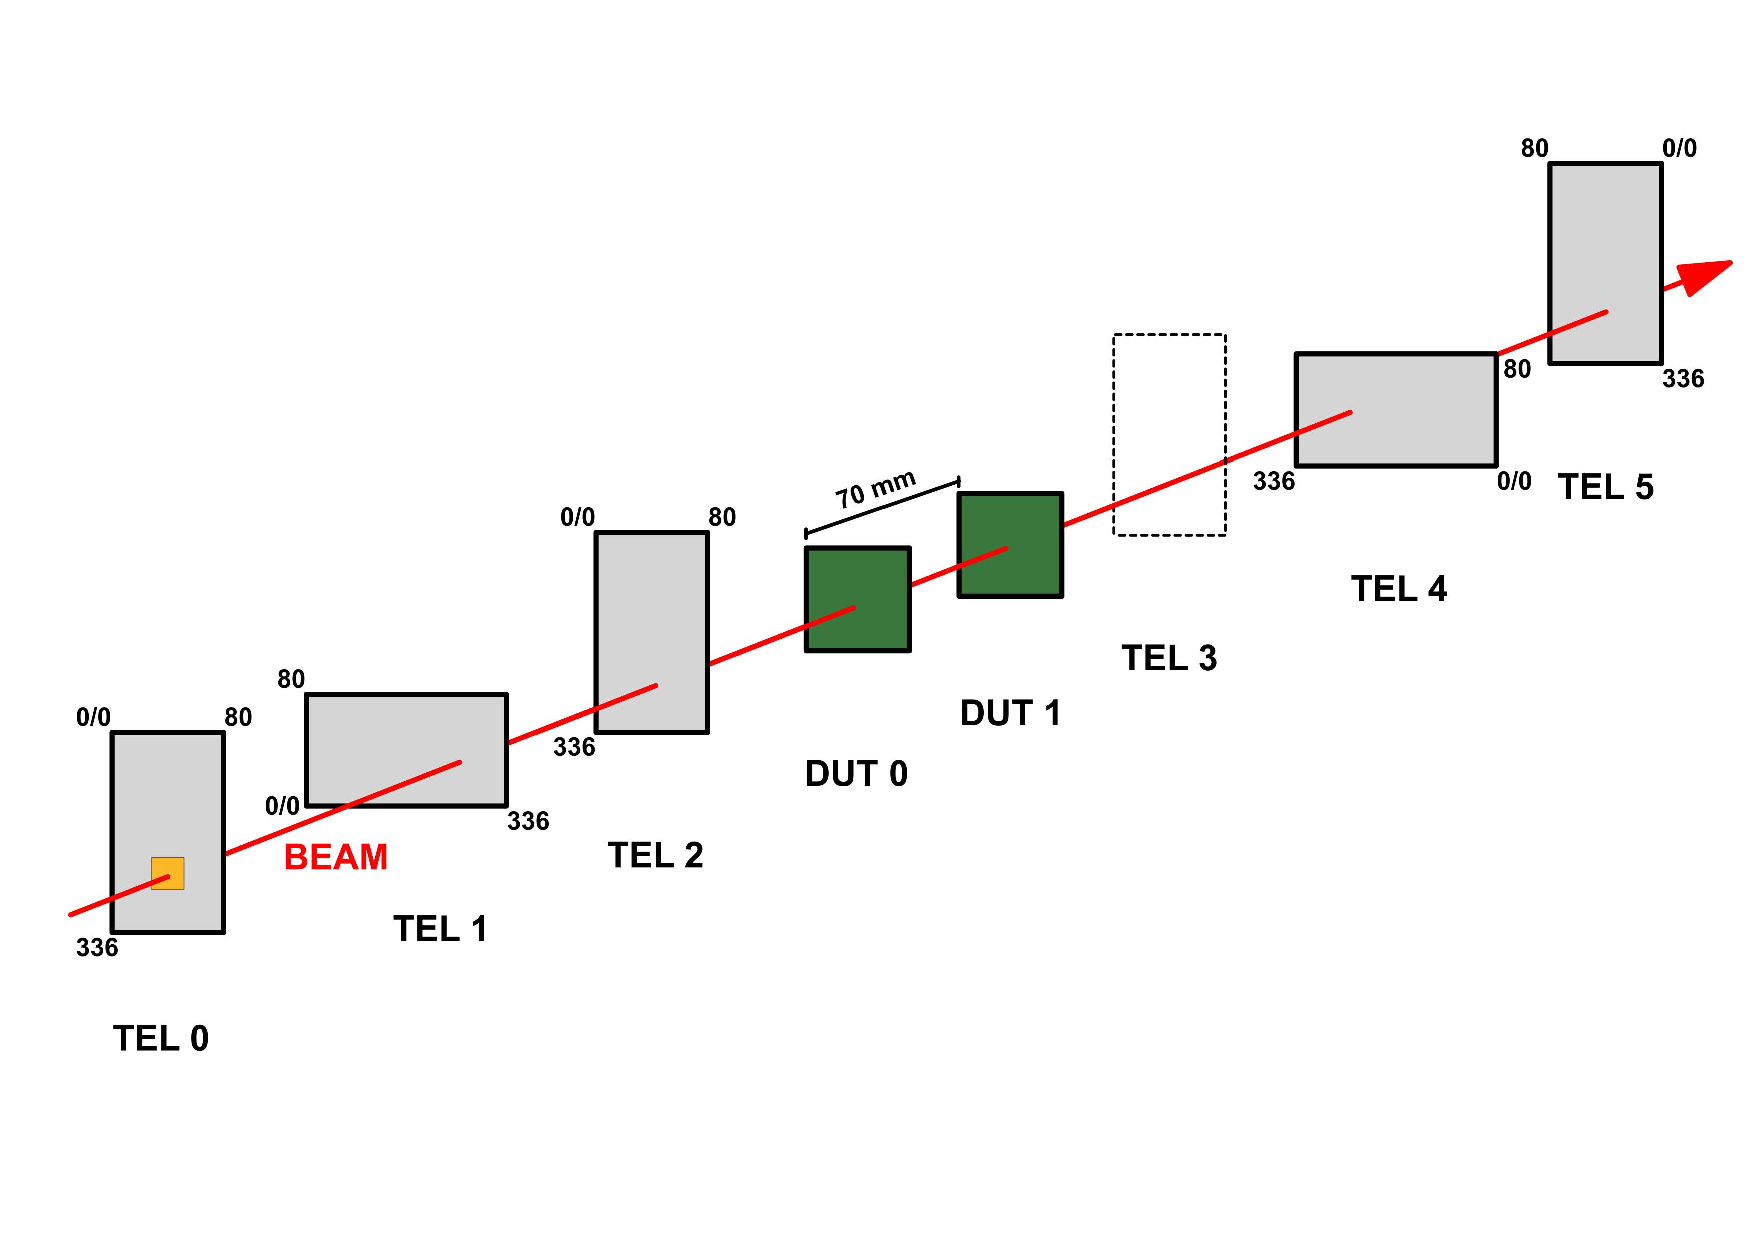
\includegraphics[width=.75\textwidth,trim=0 0 0 0]{./Figures/Setup_reprint.pdf}
%\caption{\label{fig:Setup} Schematic view of the experimental setup, showing the five FEI4 telescope \cite{Benoit_2016} planes that were operated and the two DUTs in green. Plane TEL3 was not operational during this testbeam measurement. The FEI4 readout chip has a a matrix of $ 80 \times 336 $ pixels with a pixel size of $ 250 \times 50 ~\si{\micro\meter\squared} $. The telescope planes are alternatively rotated by 90$^\circ$  to optimise the space resolution on the two transversal directions. A region of interest, shown by the  yellow area, was imposed to the first plane of the telescope, and was put in coincidence with the last telescope plane to generate the trigger.}
%\end{figure}
%
%The analysis of the data was performed using the full waveform information acquired by the oscilloscopes. The signals from the DUTs were delayed to guarantee that they were always in the second half of the waveform time window acquired by the oscilloscope.
%This configuration allowed using the first half of the waveform to determine the voltage noise $\sigma_V$ at the output of the analog front-end and set a discrimination threshold $ V_{th} $ as a multiple of the voltage noise, independently for the two DUTs. Figure~\ref{fig:waveform} shows a typical waveform with a signal pulse from a MIP at the working point with  $ \ipreamp = \SI{150}{\micro\ampere} $. The dashed line represents the discrimination threshold at $V_{th}=6~\sigma_{V}$.
%
%\begin{figure}[!htb]
%%\centering % \begin{center}/\end{center} takes some additional vertical space
%%\centering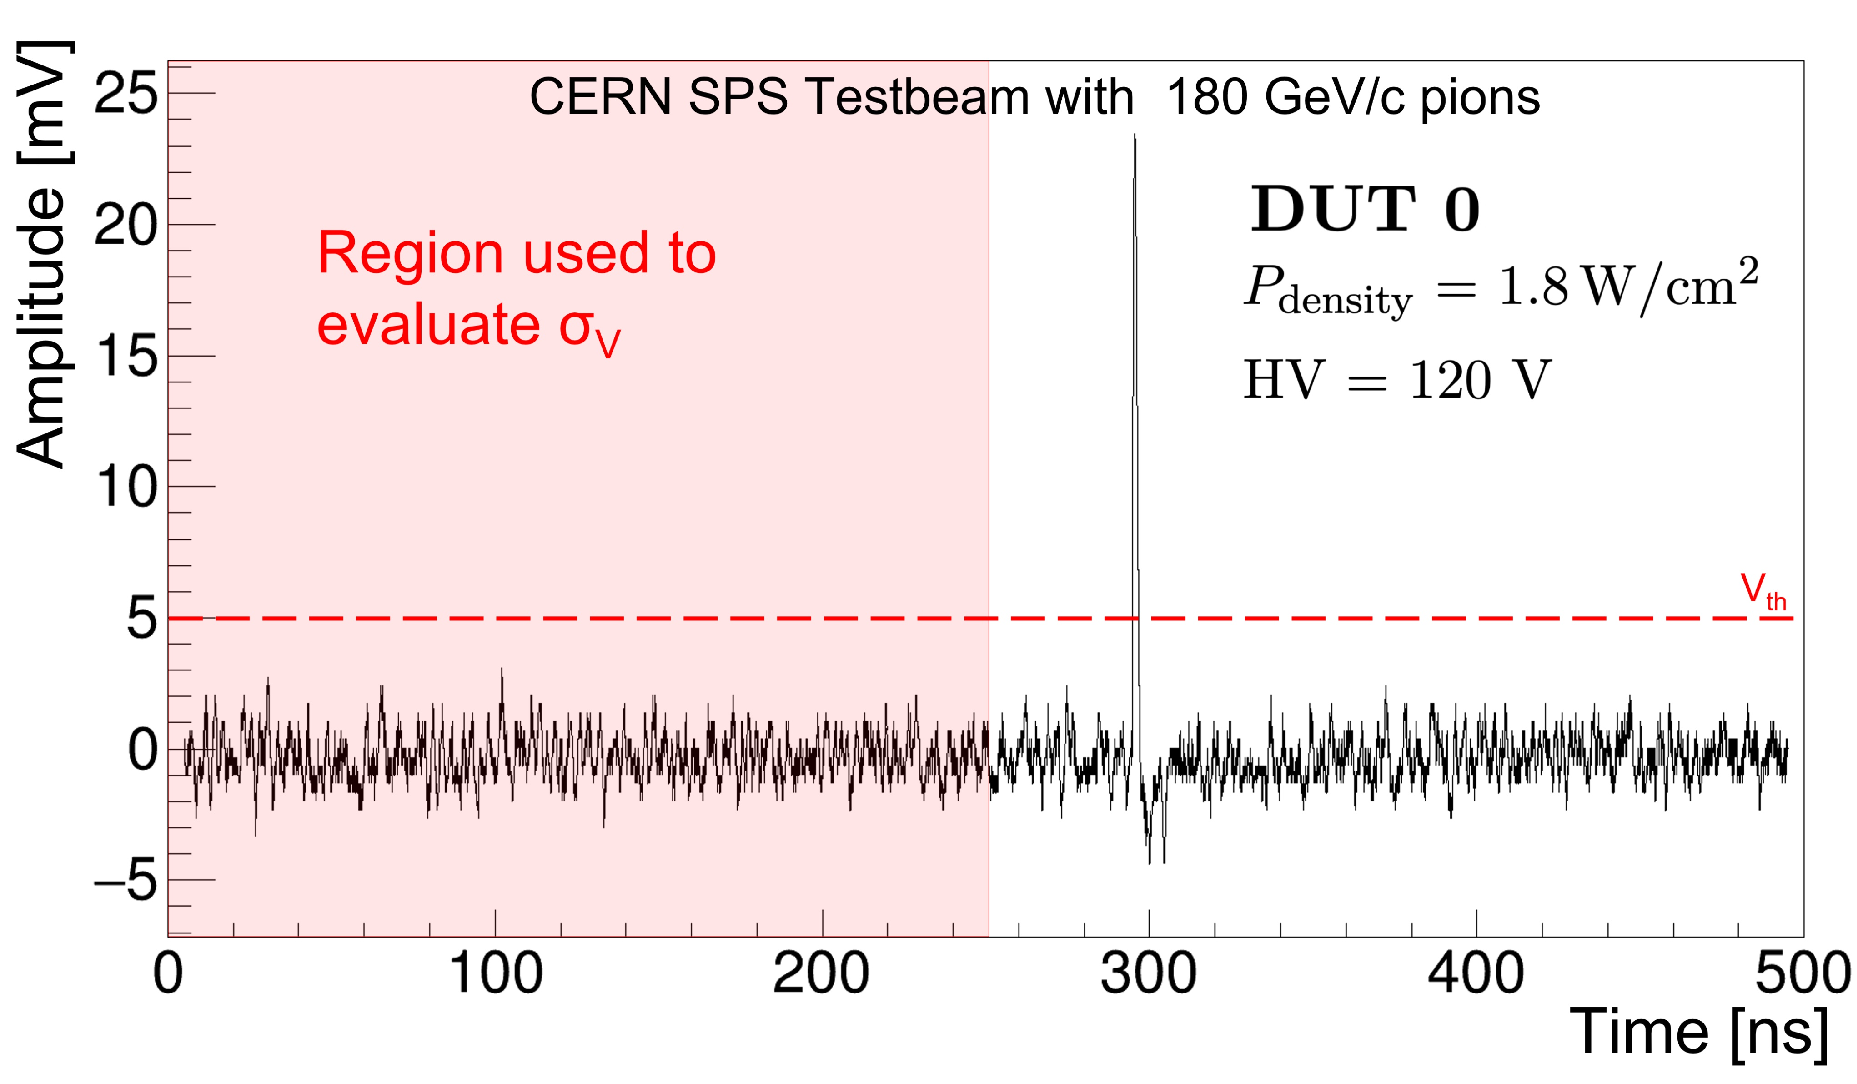
\includegraphics[width=.80\textwidth,trim=10 10 10 10]{./Figures/Waveform_analysis.png}
%\caption{\label{fig:waveform} Example of a waveform from working point $ \ipreamp = \SI{150}{\micro\ampere} $. The shaded region below 250 ns is the portion of the waveform used to extract $\sigma_{V}$. The dashed line shows the discrimination threshold used for this working point.
%}
%\end{figure}
%
%The FEI4 telescope provided the trigger to the oscilloscopes. A Region Of Interest (ROI) of $ 250 \times 600 $  \si{\micro\meter\squared} was set on one of the trigger planes of the telescope, centered around the pixels OA0 of the two DUTs that were aligned with respect to the beamline and used for the TOF measurement.
%
%Data were acquired 
%with DUT0 and DUT1
%%with the monolithic prototype ASICs 
%at the same four front-end working points used for the characterization of the DUTs  with radioactive sources (Section \ref{sec:calibrations}) for a bias voltage of 120 V. At this potential the substrate is not fully depleted. The depletion depth is estimated to be $ \SI{23}{\micro\meter} $, which corresponds to a most probable charge $ Q_{MPV} \approx 1300 $ electrons for a MIP. 
%
%A high voltage scan was also performed  only for the working point $\ipreamp = $ \SI{150}{\micro\ampere}.
%
%
%To evaluate  the efficiency and time resolution of our DUTs in the cleanest possible way, a selection was applied on the quality of the tracks reconstructed by the FEI4 telescope.
%%to achieve the best possible track reconstruction. 
%The selection consisted in discarding  events in which more than one track was reconstructed by the telescope, and in accepting only those events with the reconstructed track having an associated hit  in each of the five telescope planes and a  $ \chi^{2}/NDF \le 1 $. 
%About 30\% of the triggered events survived this stringent selection on the tracks from the telescope.
%
%For this final sample the telescope pointing resolution on the DUT planes was estimated to be  approximately 10 $\mu$m \cite{mateus_thesis}.
%
%\subsection{Cross talk and robustness to induced noise}
%\label{subsec:crosstalk}
%During laboratory and testbeam measurements,  cross talk between the channels was observed for  events with  large charge deposition,
%corresponding to approximately five times the MIP most probable charge. The analysis of these events showed that this cross talk was not influenced by the relative position of the pixels within the matrix or the routing of the signal before and after the amplification. Therefore the observed cross talk could be ascribed to two possible causes. The first is a feedback path passing through the ground of the board, which is then injected to the backside of the chip through the HV decoupling capacitors and finally in the amplifier input. This hypothesis is supported by the fact that the system becomes less stable at bias voltages below \SI{50}{\volt}, when the pixel capacitance is significantly larger. The second cause is noise induced by the driver pulse propagating in the power supply,
%since in this prototype the analog and driver electronics share the same supply lines.
%%caused by a design flaw: the sharing between the analog and driver power supplies.
%
%As a consequence of this cross talk, only  events in which the pixel under test had the largest signal among the three acquired pixels were selected for the time resolution measurement. No selection was applied for cross talk in the efficiency measurement, since cross talk appears only for efficient events.
%
%\subsection{Efficiency measurement}
%%An efficient events is defined as \textcolor{red}{an event for which at least one of the pixels crosses the discrimination threshold and the pion track is reconstructed by the FEI4 telescope at a distance of less than 3 times the telescope resolution from the edge of an active pixel.}
%For the calculation of the efficiency, all the selected pion tracks reconstructed by the FEI4 telescope were extrapolated to the surface of each of the two DUTs. Only the tracks crossing a DUT within the  area of the three pixels under study, or outside the  external edges of the pixels by at most one standard deviation of the telescope resolution, were retained.
%An event was considered efficient if the signal in at least one of the pixels crossed the discrimination threshold.
%
%Figure \ref{fig:effmap} shows the efficiency map for the two DUTs at the $\ipreamp =$ \SI{150}{\micro\ampere} working point, for a threshold of $ 6\sigma_{V} $ and a sensor bias $HV = $ 120 V. 
%The panels show the efficiency map for the entire surface of the three pixels (the pixel edges are represented by the black lines). The degraded efficiency measured nearby the twelve external sides of the hexagonal pixels is produced by the FEI4 telescope resolution, as attested by the fact that such degradation of the efficiency is not observed in the region of the three internal hexagon sides between the  pixels.
%%The map shows high efficiency both at the center of the pixels and in the interpixel regions between the three pixels under test. 
%To avoid biases stemming from the pointing resolution of the FEI4 telescope, the measurement of the detection efficiency was restricted to events with tracks extrapolated inside
%the triangular area\footnote{It should be noted that this triangular area constitutes exactly one sixth of the total area of the three pixels, which is representative of all the zones of a pixel (central-pixel zone; zone in between two pixels; zone in between three pixels) in the right geometrical proportions. Therefore, the efficiency measured inside it provides a reliable estimation of the efficiency over the entire hexagonal pixel area, unbiased by the telescope resolution.} 
%in between the three pixels that is delimited by the red lines in Figure \ref{fig:effmap}. 
%
%%a representative region of the area under test was identified (triangular region visible in the bottom left and bottom right plots of Figure \ref{fig:effmap}), which contains the central and inter-pixel regions of the pixels with the same proportion of a large matrix.
%
%\begin{figure}[!htb]
%\centering
%%\centering % \begin{center}/\end{center} takes some additional vertical space
%%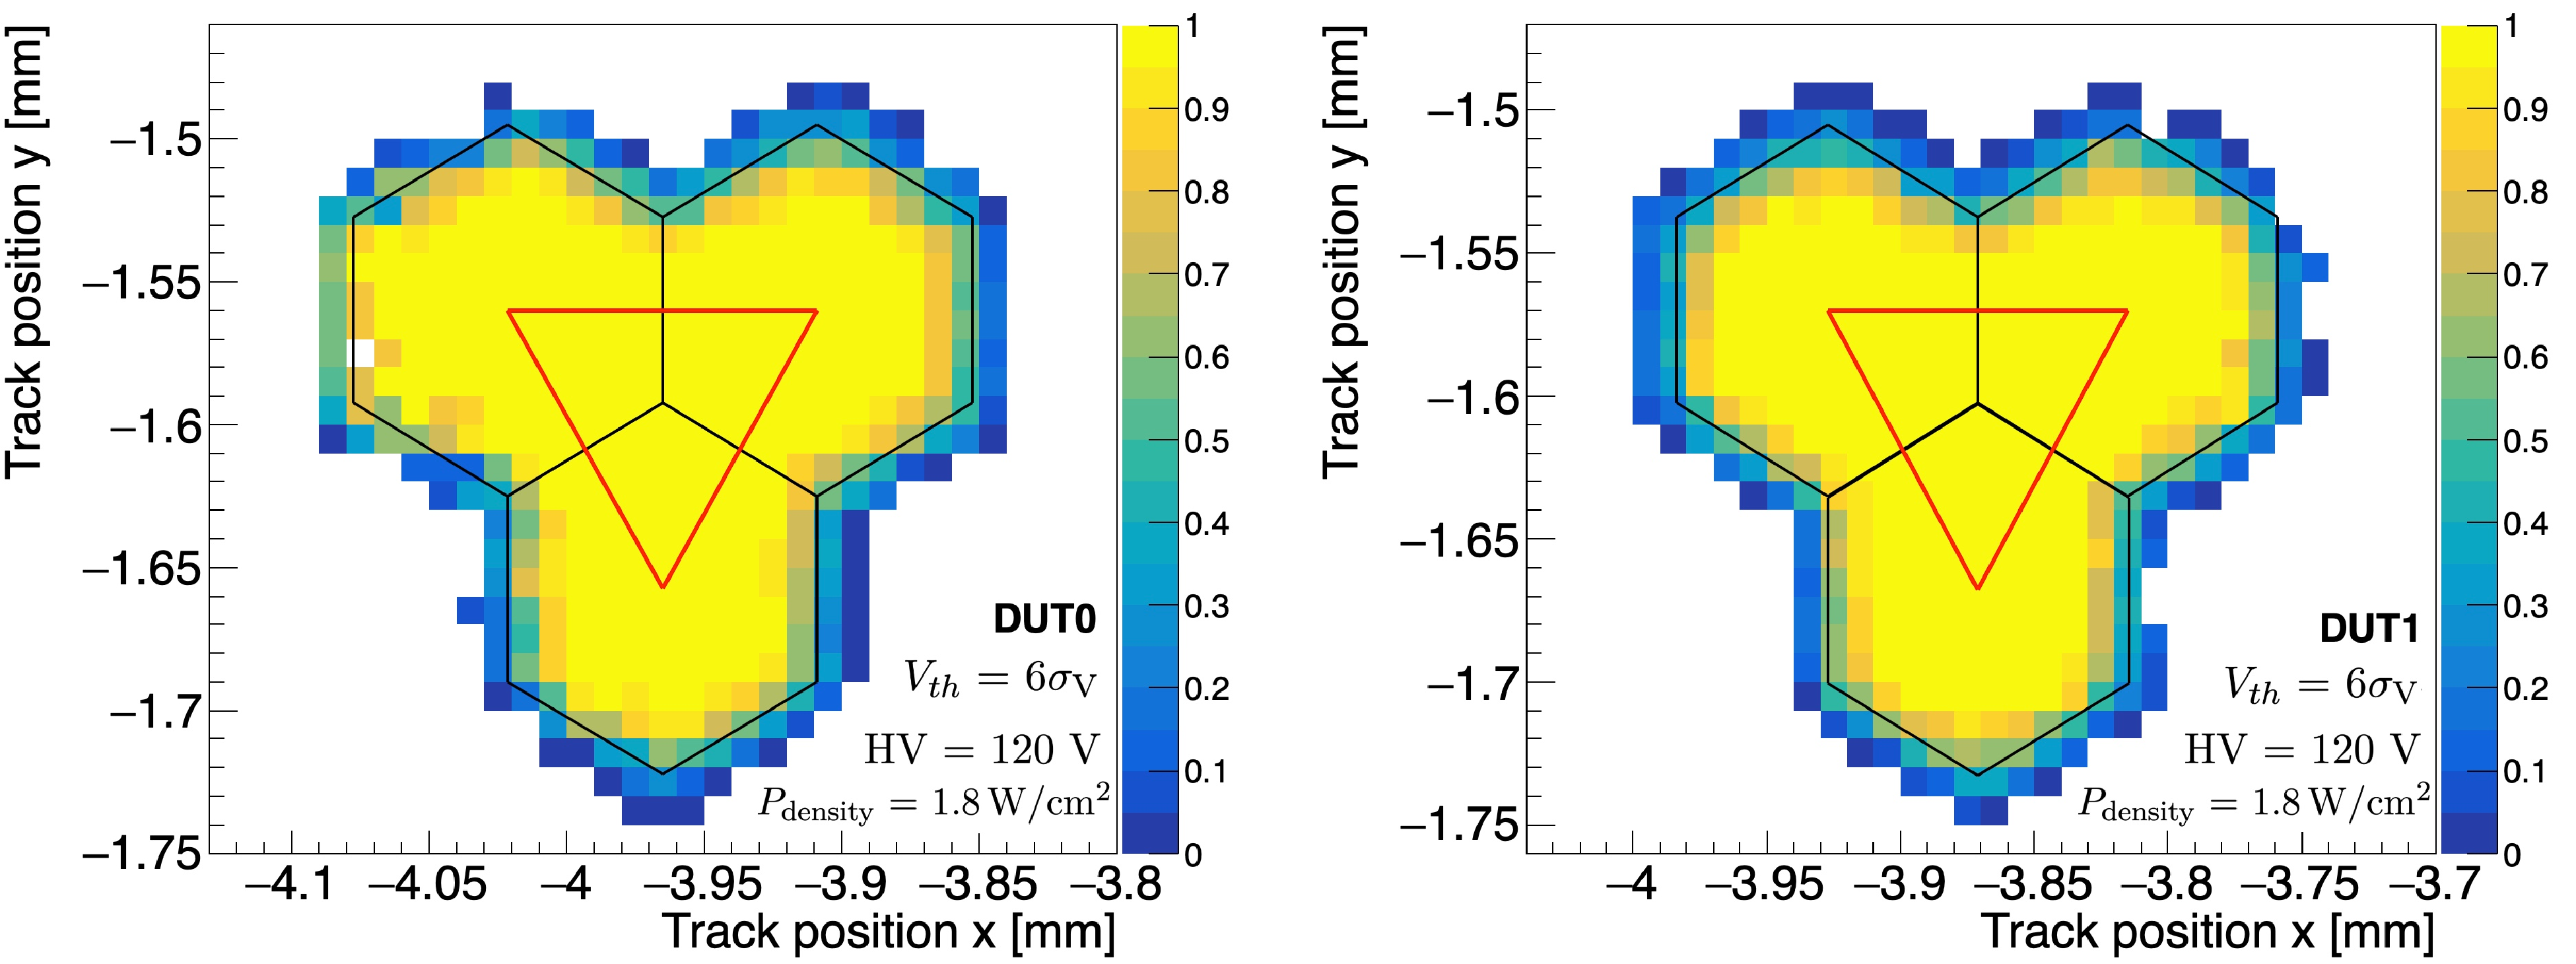
\includegraphics[width=.99\textwidth,trim=0 0 0 0]{./Figures/EfficiencyMap_120V_150uA.png}
%\caption{\label{fig:effmap} Efficiency map measured for DUT0 (left) and DUT1 (right) at $ \ipreamp = \SI{150} \mu$A, threshold $ V_{th} = 6 ~\sigma_{V}$ and $ HV = \SI{120}{\volt} $. 
%The pixel edges are shown by the black lines.
%The  efficiency degradation around the external edges of the three pixels is due to the FEI4 telescope resolution.
%The efficiency measured inside the triangular area delimited by the red lines is unaffected by the telescope pointing resolution and is used throughout this study.
%%The bottom panels show the efficiency maps for a triangular region in between the pixels (one sixth of the area of the three pixels), that is unaffected by the telescope resolution (yellow = higher than 99.5$\%$). 
%}
%\end{figure}
%
%Figure~\ref{fig:effipreampscan} and Table \ref{tab:efftable} show the efficiency obtained within the triangular  area for the four preamplifier working points at a discrimination threshold of 6 $\sigma_V$ and at a sensor bias voltage of 120 V. The efficiency follows the trend expected from the ENC measurement of Table~\ref{tab:gaintable}.  All the preamplifier working points show an efficiency well above 99\% except for the one at \SI{7}{\micro\ampere}. At this current a larger depletion depth would be required to operate the front-end at even higher efficiency. It is also noted that DUT0 shows a lower efficiency, compatibly with the larger ENC measured with the $ \Cd $ source (Section~\ref{sec:calibrations}). At higher currents  DUT0 is slightly more efficient than  DUT1. To investigate this difference, the efficiency as a function of the discrimination threshold was inspected.
%The results are reported in Figure \ref{fig:effthrscan} for $ HV = \SI{120}{\volt} $.
%The threshold scan indicates a clear difference in performance, in spite of the fact that both DUTs reach the efficiency plateau at a threshold of six standard deviations of the noise. 
%\begin{figure}[!htb]
%\centering % \begin{center}/\end{center} takes some additional vertical space
%%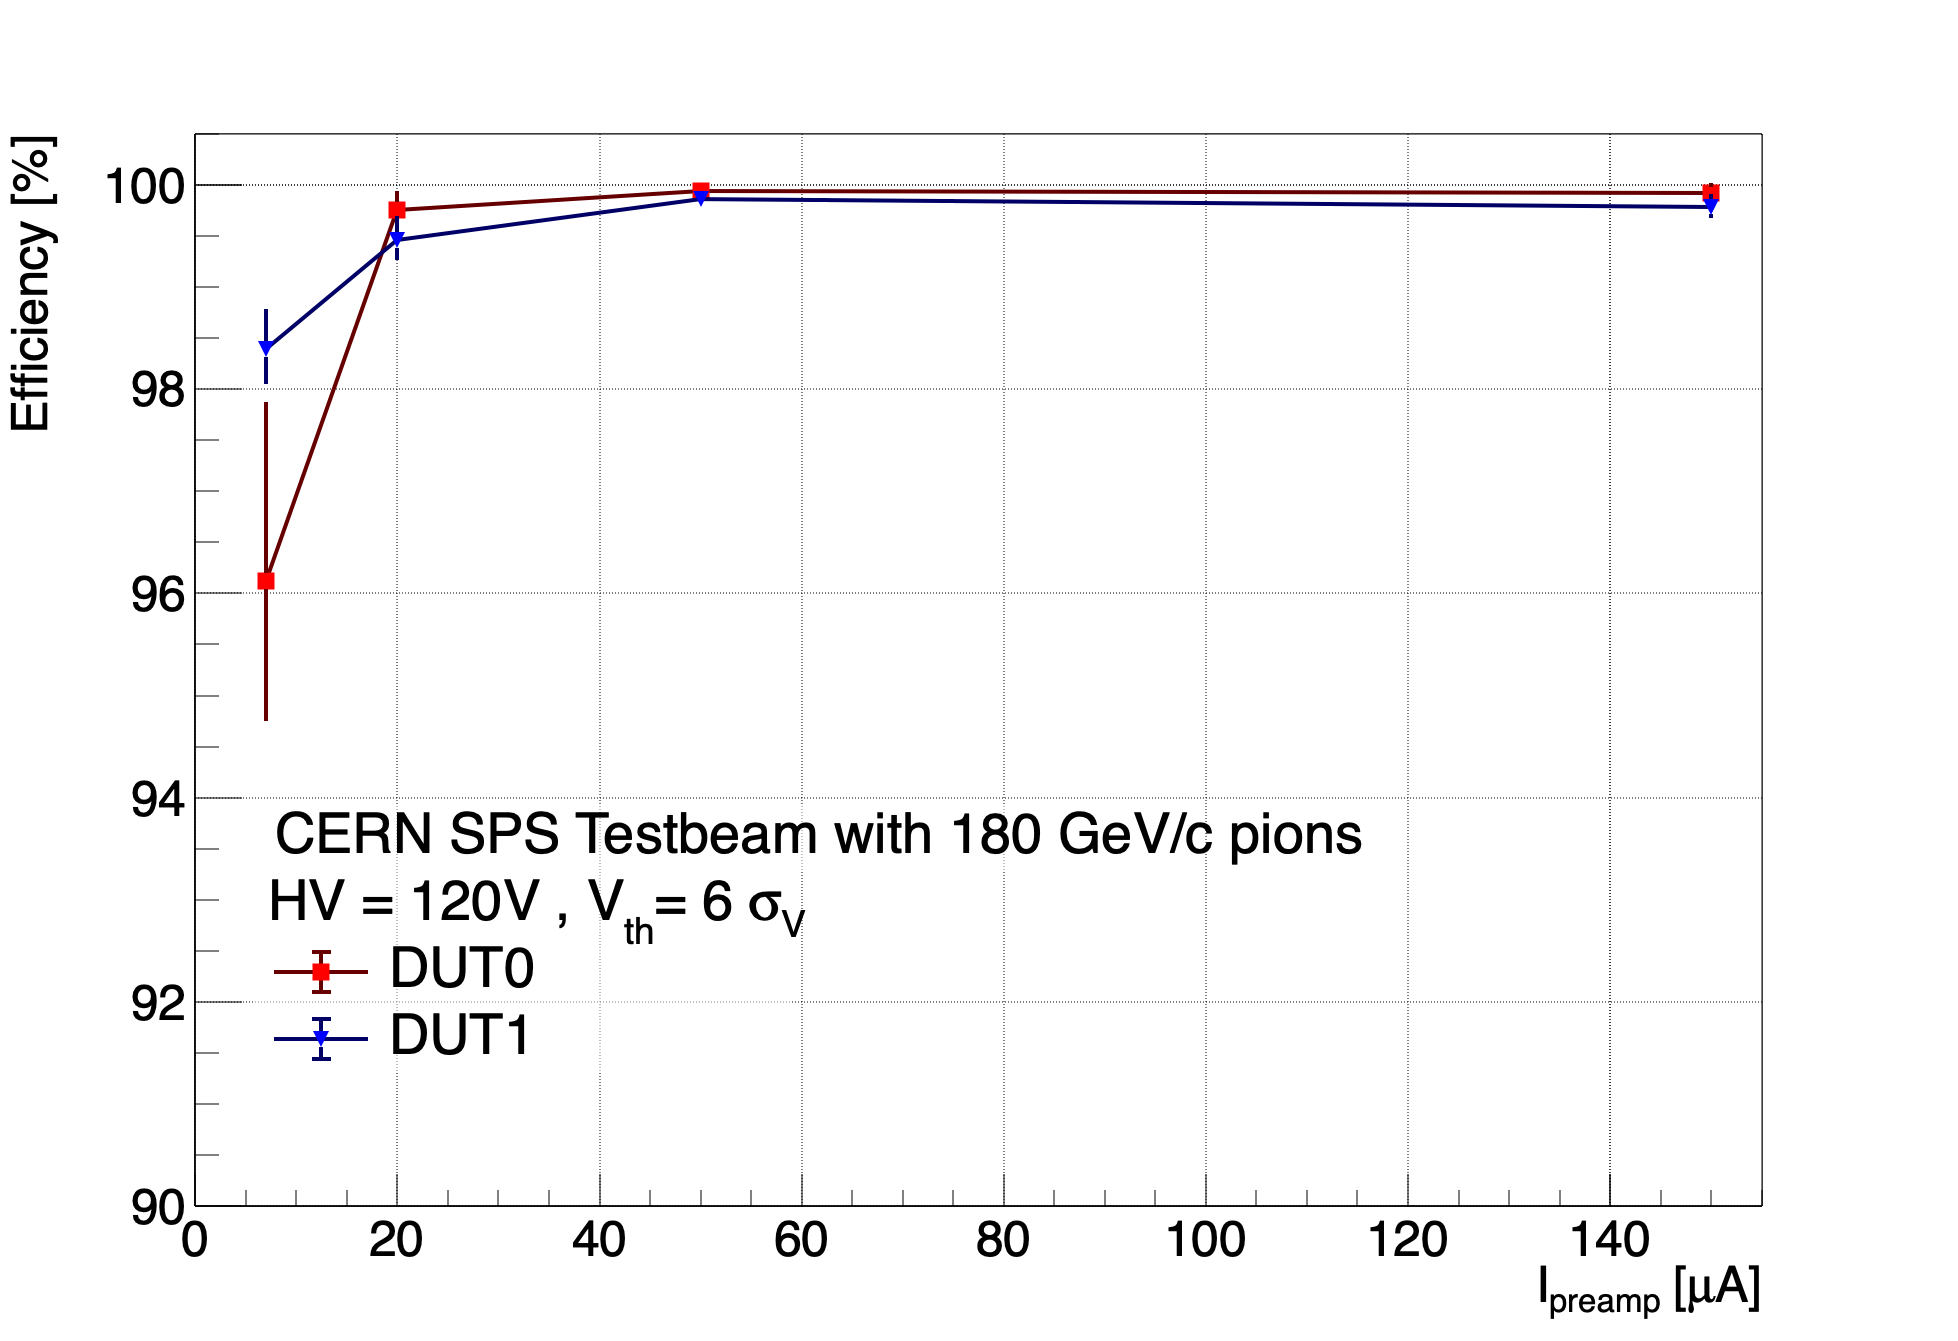
\includegraphics[width=.7\textwidth,trim=0 0 0 0]{./Figures/Efficiency_Ipreamp_Scan.png}
%\caption{\label{fig:effipreampscan} Efficiency vs. $ \ipreamp $ for $ HV = \SI{120}{\volt} $, evaluated in the triangular inter-pixel zone for  DUT0 (in red) and DUT1 (in blue).}
%\end{figure}
%
%\begin{table}[!htb]
%\centering
%\renewcommand{\arraystretch}{1.3}
%\begin{tabular}{c|cccc|l}
%\cline{1-5}
%\multicolumn{5}{|c|}{Efficiency measured at HV = 120 V}                                                                                                                         & \multicolumn{1}{c}{\textbf{}} \\ \cline{1-5}
%%                            & \multicolumn{1}{c|}{7 µA}                 %  & \multicolumn{1}{c|}{20 µA}                     & %\multicolumn{1}{c|}{50 µA}                     & 150 µA                 %   &                               \\ \cline{1-5}
%\multicolumn{1}{|c|}{$\ipreamp$ [$\mu$A]} & \multicolumn{1}{c|}{7} & \multicolumn{1}{c|}{20} & \multicolumn{1}{c|}{50} & 150 &                               \\ \cline{1-5}
%\multicolumn{1}{|c|}{Efficiency DUT0 {[}\%{]}} & \multicolumn{1}{c|}{$ 96.1_{-1.7}^{+1.4} $} & \multicolumn{1}{c|}{$ 99.75_{-0.17}^{+0.12} $} & \multicolumn{1}{c|}{$ 99.94_{-0.05}^{+0.03} $} & $ 99.91_{-0.08}^{+0.05} $ &                               \\ \cline{1-5}
%\multicolumn{1}{|c|}{Efficiency DUT1 {[}\%{]}} & \multicolumn{1}{c|}{$ 98.4_{-0.4}^{+0.3} $} & \multicolumn{1}{c|}{$ 99.45_{-0.2}^{+0.2} $}   & \multicolumn{1}{c|}{$ 99.86_{-0.07}^{+0.05} $} & $ 99.78_{-0.11}^{+0.08} $ &                               \\ \cline{1-5}
%\end{tabular}
%\caption{Efficiency of the two DUTs at different $\ipreamp$ for $ HV = \SI{120}{\volt}$. The efficiency is measured according to the definition given in the text. The uncertainties are statistical only.}
%\label{tab:efftable}
%\end{table}
%
%\begin{figure}[!htb]
%\centering % \begin{center}/\end{center} takes some additional vertical space
%%\includegraphics[width=.65\textwidth,trim=0 0 0 0]{./Figures/EfficiencyScan_120V_150uA.png}
%\caption{\label{fig:effthrscan} Efficiency vs. discrimination threshold measured within the triangular inter-pixel zone for  DUT0 (in red) and DUT1 (in blue).}
%\end{figure}
%
%
%\begin{figure}[!htb]
%\centering % \begin{center}/\end{center} takes some additional vertical space
%%\includegraphics[width=.65\textwidth,trim=0 0 0 0]{./Figures/Efficiency_HV_Scan.png}
%\caption{\label{fig:effHVscan} Efficiency vs. \!\!sensor bias voltage for the two DUTs at $\ipreamp$ = 150 $\mu$A and voltage threshold of 6 $\sigma_V$. The vertical error bars show the statistical uncertainties.}
%\end{figure}
%
%
%
%
%
%
%
%
%\begin{table}[!htb]
%\centering
%\renewcommand{\arraystretch}{1.3}
%\begin{tabular}{c|ccccc|l}
%\cline{1-6}
%\multicolumn{6}{|c|}{Efficiency measured at $\ipreamp = 150\mu A$}                                                                                                                         & \multicolumn{1}{c}{\textbf{}} \\ \cline{1-6}
%\multicolumn{1}{|c|}{HV [V]} & \multicolumn{1}{c|}{80} & \multicolumn{1}{c|}{100} & \multicolumn{1}{c|}{120} &\multicolumn{1}{c|}{140} & 160 &                               \\ \cline{1-6}
%\multicolumn{1}{|c|}{Efficiency DUT0 {[}\%{]}} & \multicolumn{1}{c|}{$ 98.97_{-0.46}^{+0.35} $} & \multicolumn{1}{c|}{$ 99.78_{-0.26}^{+0.14} $} & \multicolumn{1}{c|}{$ 99.91_{-0.08}^{+0.05} $} &\multicolumn{1}{c|}{$ 99.81_{-0.71}^{+0.18} $} & $ 99.95_{-0.18}^{+0.04} $ &                               \\ \cline{1-6}
%\multicolumn{1}{|c|}{Efficiency DUT1 {[}\%{]}} & \multicolumn{1}{c|}{$ 96.70_{-0.70}^{+0.61} $} & \multicolumn{1}{c|}{$ 99.21_{-0.37}^{+0.28} $}   & \multicolumn{1}{c|}{$ 99.78_{-0.11}^{+0.08} $} &\multicolumn{1}{c|}{$ 100._{-0.42}^{+0.00} $} & $ 99.88_{-0.20}^{+0.09} $ &                               \\ \cline{1-6}
%\end{tabular}
%\caption{Efficiency at different HV values for the two DUTs for $\ipreamp$ = 150 µA. The efficiency is measured according to the definition given in the text. The uncertainties are statistical only.}
%\label{tab:efftablehv}
%\end{table}
%
%The efficiency measurement of a sensor HV scan carried out for the working point  $ \ipreamp = \SI{150}{\micro\ampere} $ is reported in Figure~\ref{fig:effHVscan} and Table~\ref{tab:efftablehv}. 
%The scan shows that the two DUTs are in the efficiency plateau at 120 V. At the \SI{50}{\ohm\cm} substrate resistivity of this prototype, increasing the HV from \SI{120}{\volt} to \SI{160}{\volt} increases the depletion depth by 15\%, which has little or no contribution for the working point at the highest power consumption, but  could have been beneficial for the front-end operation at \SI{7}{\micro\ampere} for which a small drop in efficiency was observed (Figure~\ref{fig:effipreampscan}).
%
%\subsection{Time resolution measurement}
%For the time resolution measurement, the pixels OA0 of the two DUTs were carefully aligned with respect to the beamline and events in which the two pixels registered signals with amplitudes above a 
%discrimination threshold of $ 6~\sigma_V $ in coincidence were selected.
%%coincidences between pixels OA0 of the two DUTs were selected applying a discrimination threshold of $ \approx6\sigma_V $. 
%Furthermore, the telescope-track quality selection described in Section~\ref{subsec:dataset} and the cross-talk selection described in Section~\ref{subsec:crosstalk} were applied. To avoid biasing the sample with a geometrical selection, no requirement on the telescope-track position was imposed.
%
%\begin{figure}[!htb]
%\centering %
%%\includegraphics[width=.92\textwidth,trim=5 0 670 0, clip]{./Figures/TimeRes_WP7_160V.png}
%\caption{\label{fig:TWcorr} Distributions of the difference in TOA between the two DUTs vs. the inverse of the amplitude that was used for the time-walk correction of DUT0 (left) and DUT1 (right). Both DUTs were operated at $ \ipreamp = \SI{150}{\micro\ampere} $ and $ HV = \SI{160}{\volt} $. The time-walk correction points (in red) were obtained by  a Gaussian fit on each bin of the inverse of the amplitude. The red segments show the  linear interpolation between the time-walk correction points used to correct the data.
%%, which were associated at the average value of each bin, that were used to correct for time walk. 
%The TOA difference contains an arbitrary offset that is irrelevant for the measurement of the time resolution.}
%\end{figure}
%
%
%%\subsubsection{Time-walk correction}
%{\it Time-walk correction} 
%
%Figure \ref{fig:TWcorr} shows the 
%%time-walk correction 
%difference in the Time-Of-Arrival (TOA) measured in pixels OA0 of  DUT0 (TOA0) and DUT1 (TOA1) as a function of the inverse of the signal amplitude in DUT0 (left) and DUT1 (right)
%for the working point at \SI{150}{\micro\ampere} and $ HV = \SI{160}{\volt}$.
%%, for which the best results in terms of time resolution are expected. 
%The data show a large variation of the average of the difference  TOA0$-$TOA1  as a function of the signal amplitudes, of the order of a few hundreds ps, that was corrected in the following way. 
%
%
%The data were divided in variable-size bins of the inverse of the amplitude containing at least 200 entries. For each of these bins for DUT0 in Figure \ref{fig:TWcorr} left, the most probable value of TOA0-TOA1 was obtained by  a Gaussian fit (red points in the figure). That value was associated to the average value of the inverse of the DUT0 amplitude distribution within that bin (instead than to the center of the bin).
%%and was used to obtain the time-walk correction value for that bin. 
%An event-by-event correction was then applied to the inverse of the amplitude of the  signal in DUT0, using the value provided by the linear interpolation (red segments in the figure) of the two adjacent  time-walk correction points.
%Once DUT0 was time-walk corrected in this way, the entire procedure was repeated for DUT1 (shown in Figure \ref{fig:TWcorr} right) to complete the time-walk correction\footnote{Given its importance for this measurement, the time-walk correction was performed also with an unbinned maximum-likelihood fit. This second method was used for a simultaneous extraction of the  resolution parameter \sigtoa and of the two  time-walk correction functions for DUT0 and DUT1. For all the data samples analysed, the results  were within few percent from those obtained by the method described in the text.}.
%
%
%{\it Extraction of the time resolution} 
%
%%\subsection{Time resolution measurement}
%Once  data were corrected for time walk,
%Gaussian fits were performed to the TOA0-TOA1 distributions,  including only  bins containing more than 25\% of the entries at the maximum  of the distribution. It was then assumed that the two DUTs have the same resolution, so that the time resolution of each DUT can be estimated as $\sigma_{t} = \sigma\_{\it TOA0-TOA1}/\sqrt{2}$.
%%\begin{equation}
%%    \sigma_{t} = \frac{\sigma\_{\it TOA0-TOA1}}{\sqrt{2}} 
%%\end{equation}
%
%As an example, Figure \ref{fig:TOF} shows the resulting TOA difference distribution after time-walk correction for the data acquired at the working points  \SI{150}{\micro\ampere} and $ HV = \SI{160}{\volt}$ (left) and 7 $\mu$A and 120 V (right).  In the case of the former, that is the  best working point for time resolution, the standard deviation obtained by the Gaussian fit is measured to be $ \sigma\_{\it TOA0-TOA1}= (51.4 \pm 1.1) $ ps. 
%Therefore the time resolution of each DUT is estimated to be
%\begin{equation}
%    \sigma_{t} = \frac{\sigma\_{\it TOA0-TOA1}}{\sqrt{2}} = (36.4 \pm 0.8) \si{\pico\second}.
%\end{equation}
%\begin{figure}[!htb]
%\centering %
%%\includegraphics[width=.47\textwidth,trim=1315 0 40 60, clip]{./Figures/TimeRes_WP7_160V.png}
%\qquad
%%\includegraphics[width=.47\textwidth,trim=1315 0 40 60, clip]{./Figures/TimeResolution_120V_7uA.png}
%\caption{\label{fig:TOF} TOA difference between pixels OA0 of DUT0 and DUT1 after time-walk correction for the two working points reported in the panels. 
%%The left panel shows the data acquired at $\ipreamp = \SI{150}{\micro\ampere}$ and $ HV = \SI{160}{\volt}$. The right panel shows the results at $\ipreamp = \SI{7}{\micro\ampere}$ and $ HV = \SI{120}{\volt}$. 
%A constant arbitrary offset is present, which is irrelevant for the time-resolution calculation. The  red lines show the results of the Gaussian fit using only the bins with more than 25\% of the entries in the maximum of the distribution. 
%The full red lines show the ranges used for the fits, while the dashed red lines allow the estimation of the non-Gaussian components in the tails.}
%%The dashed red lines show the non-Gaussian component in the tails.}
%\end{figure}
%The fraction of events exceeding the Gaussian fit in the tails of the distribution of Figure \ref{fig:TOF} is approximately 5\%. This fraction of events represents the typical non-Gaussian component found in the tails of the time-resolution distribution for  all the data sets acquired at the testbeam at different sensor and preamplifier bias.
%As a consequence the resolutions quoted in the following refer to 95\% of the signals acquired by the DUTs.
%
%Figure \ref{fig:TOFHV} top shows the time resolution as a function of the HV for the highest power consumption working point   $ \ipreamp = \SI{150}{\micro\ampere} $. %The result suggests that the detector is entering the  time-resolution plateau at $ HV = \SI{140}{\volt} $. 
%The time resolution varies between 60 and 36 ps with the HV between 80 and 160 V.
%At $ HV = \SI{120}{\volt} $ the timing performance is approximately 20\% worse than the one measured at 160 V.
%
%Figure \ref{fig:TOFHV} bottom shows the time resolution measured at $ HV = \SI{120}{\volt} $  for the  four $\ipreamp$ working points. As expected, the time resolution depends on the preamplifier current. A significant degradation of the performance is observed for the lowest power-consumption working point studied $\ipreamp = $  \SI{7}{\micro\ampere}, for which the time resolution still remains  at the level of 200 ps.
%
%\vspace{5pt}
%\begin{figure}[!htb]
%\centering %
%%\includegraphics[width=.65\textwidth,trim=0 0 0 0, clip]{./Figures/TimeResolution_HV_Scan.png}
%
%\vspace{10pt}
%%\includegraphics[width=.65\textwidth,trim=0 0 0 0, clip]{./Figures/TimeResolution_Ipreamp_Scan.png}
%\caption{\label{fig:TOFHV} Top: time resolution as a function of sensor bias voltage at $ \ipreamp = \SI{150}{\micro\ampere}$. 
%Bottom: time resolution as a function of $ \ipreamp $ for sensor bias voltage $HV = $ 120 $V$.
%The time resolution is defined as $(\sigma\_{\it TOA0-TOA1})/\sqrt{2}$. It refers to the Gaussian component of the data, which is approximately 95\% of the total.}
%\end{figure}
%
%
%
%
%
%
%
%
%
%
%
%
%
		\subsection{Detection efficiency \textcolor{red}{ 4 pages}}
%%Detection of MONOLITH
%
%The pion tracks reconstructed by the FEI4 telescope and surviving the analysis selection criteria were used to measure the DUT detection efficiency. The efficiency was computed as the ratio between the number of selected tracks associated to recorded signals with amplitudes above a threshold of 7 times the voltage noise $\sigma_V$ and the total number of selected tracks traversing the DUT in the area corresponding to the four analog pixels. A tolerance of $\SI{10}{\um}$ in the region outside the external boundaries of the four-pixel area was allowed to account for the finite telescope pointing resolution.
%
%\begin{figure}[!htb]
%\centering
%\includegraphics[width=.49\textwidth,trim=0 0 0 0]{./Figures/WP1_HV200V_efficiency_map.pdf}
%\includegraphics[width=.49\textwidth,trim=0 0 0 0]{./Figures/WP1_HV200V_triangles_map.pdf}
%\caption{\label{fig:effmap} Detection efficiency measured for the \monolith\ prototype operated at power density $P_{\mathrm {\it density}} =$ 2.7 W/cm$^2$ and $HV=\SI{200}{\volt}$, with a discrimination threshold $V_{\mathrm {\it th}}=7~\!\sigma_V$. In the left panel, the measurement is performed in a region that extends beyond the pixel edges (black lines) by $\SI{10}{\um}$. The apparent decrease of the efficiency  at the external boundaries delimiting the area of the four instrumented pixels is produced by the finite FEI4 telescope pointing resolution. 
%The right panel shows the efficiency measured in the two triangular areas connecting the centres of pixels OA0--OA2--OA3 and OA0--OA2--OA1, which is unaffected by the resolution of the telescope; the colour scale of the plot starts at 95\% efficiency. 
%}
%\end{figure}
%
%Figure~\ref{fig:effmap} shows the results of the efficiency measurement for the DUT operated at $P_{\mathrm {\it density}} =$ 2.7 W/cm$^2$ and $HV=\SI{200}{\volt}$. As shown by the left panel, the finite FEI4 telescope pointing resolution  
%generates an apparent inefficiency close to the 14 external edges of the four pixels (and an efficiency outside them), which makes the evaluation of the efficiency in the total pixel area difficult.
%%bring within the tolerance region defined for the efficiency computation tracks that originally crossed the DUT outside the four analog pixels. This effect shows as an apparent decrease in detection efficiency. In the left panel, the bias is clearly visible at the edges of the area delimited by the four pixels. 
%Since this effect is not present in the five internal edges of the four pixels,
%the measurement was repeated selecting only tracks extrapolated inside the two triangles connecting the OA0--OA2--OA3 and OA0--OA2--OA1 pixel centres. %Tracks within the two triangles are not affected by the aforementioned bias, as shown by the right panel. 
%The result is shown in the right panel of Figure~\ref{fig:effmap}, in which the color scale starts at 95\%.
%It should be noted that the two triangles contain all the relevant pixel regions, such as the boundary between two pixels and the corner between three pixels, in the same proportion as in an entire pixel. For all the working points, the efficiencies measured separately in the two triangles were found to be compatible within statistics, and thus averaged.
%The efficiency value measured inside the two triangles for the working point of Figure~\ref{fig:effmap} is ($ 99.86_{-0.04}^{~\!+0.03} $)\%, as reported in the second row of Table~\ref{tab:eff_ipream_HV_pscan}.
%
%\begin{table}[!htb]
%\centering 
%\renewcommand{\arraystretch}{1.4}
%%%%%%%%%%%%%%%%%%%%%%%%%%%%%%%%%%%%%%%%%%%
%\begin{tabular}{|c|c|c|}
%\cline{1-3}
% $P_{\it density}$ [W/cm$^2$] & ~~~~~~~$HV$~[\si{V}]~~~~~~~  & Average efficiency [\%] \\
%\cline{1-3}
%2.7   & 250 & $ 99.80_{-0.09}^{~\!+0.07} $ \\
%2.7   & 200 & $ 99.86_{-0.04}^{~\!+0.03} $ \\
%2.7   & 160 & $ 99.71_{-0.10}^{~\!+0.08} $ \\
%2.7   & 120 & $ 99.80_{-0.09}^{~\!+0.07} $ \\
%0.9   & 200 & $ 99.83_{-0.04}^{~\!+0.04} $ \\
%0.36  & 200 & $ 99.81_{-0.05}^{~\!+0.04} $ \\
%0.13  & 200 & $ 99.77_{-0.05}^{~\!+0.04} $ \\
%0.04  & 200 & $ 99.86_{-0.07}^{~\!+0.05} $ \\
%\cline{1-3}
%\end{tabular}
%\caption{Detection efficiency measured for the \monolith\ 2022 prototype at different power density   and sensor bias voltage values. A voltage threshold of 7 times the voltage noise $\sigma_V$ is applied. The efficiencies are measured separately in the two triangular areas connecting the OA0--OA2--OA3 and OA0--OA2--OA1 pixel centers shown in Figure~\ref{fig:effmap}, and then averaged.}
%\label{tab:eff_ipream_HV_pscan}
%\end{table} 
%
%It is interesting to characterise the dependence of the detection efficiency on the discrimination threshold, as it is influenced by the signal to background ratio of the  sensor prototype. The result for the DUT operated at $P_{\mathrm {\it density}} =$ 2.7 W/cm$^2$ and $HV=\SI{200}{\volt}$ is shown in Figure~\ref{fig:effthrscan}. Remarkably, the efficiency remains above $99\%$ up to threshold values of 18 times the voltage noise $\sigma_V$. 
%A voltage threshold of $7~\!\sigma_V$ was used throughout the data analysis, which corresponds to approximately 600 electrons for this working point.
%Figure~\ref{fig:effthrscan} reports also the noise-hit rate measured in the laboratory, which is $2.9\cdot 10^{-4}$ Hz/pixel at $7~\!\sigma_V$, corresponding approximately to 1 noise hit every hour.
%In the testbeam data sample taken at this working point, we expect less than 1 noise hit.
%\begin{figure}[!h]
%\centering % \begin{center}/\end{center} takes some additional vertical space
%%\includegraphics[width=.70\textwidth,trim=0 0 0 0]{./Figures/eff_fhr_vs_thr.pdf}
%\caption{\label{fig:effthrscan} Detection efficiency (red squares) and noise-hit rate (blue squares) measured within the two triangular areas depicted in Figure~\ref{fig:effmap}, shown as a function of the voltage threshold in integer multiples of the the voltage noise $\sigma_V$. The data refer to sensor bias $ HV = \SI{200}{\volt} $ and power density $P_{\mathrm {\it density}} =$ 2.7 W/cm$^2$.
%}
%\end{figure}
%
%Table~\ref{tab:eff_ipream_HV_pscan} and Figure~\ref{fig:eff_ipream_HV_pscan} show the average efficiency in the two triangles for the eight working points at which data were acquired. 
%%Similarly, the average efficiencies are shown in Figure~\ref{fig:eff_ipream_HV_pscan} as a function of the power density $P_{\mathrm {\it density}}$ and the sensor bias voltage $HV$. 
%Within the statistical uncertainty, no significant trend is observed: all the efficiencies are found to be compatible with 99.8\%. Figure~\ref{fig:eff_radius} shows  the DUT efficiencies measured as a function of the distance from the pixel center for the eight working points acquired. In all cases the efficiencies remain remarkably stable around 99.8\% within the whole pixel area, showing that no drop in the inter-pixel region is measured.
%
%\begin{figure}[!htb]
%\centering % \begin{center}/\end{center} takes some additional vertical space
%%\includegraphics[width=.49\textwidth,trim=0 0 0 0]{./Figures/eff_HV.pdf}
%%\includegraphics[width=.49\textwidth,trim=0 0 0 0]{./Figures/eff_power.pdf}
%\caption{\label{fig:eff_ipream_HV_pscan} Detection efficiency measured within the two triangular areas depicted in Figure~\ref{fig:effmap} with $V_{\mathrm {\it th}}=7~\!\sigma_V$. In the left panel, the efficiency is measured at four values of sensor bias voltage for a power density of 2.7 W/cm$^2$. In the right panel, the measurement is shown for five power density values at sensor bias $HV=\SI{200}{\volt}$.}
%\end{figure}
%
%\begin{figure}[!htb]
%\centering % \begin{center}/\end{center} takes some additional vertical space
%%\includegraphics[width=.49\textwidth,trim=0 0 0 0]{./Figures/eff_vs_radius_HV.pdf}
%%\includegraphics[width=.49\textwidth,trim=0 0 0 0]{./Figures/eff_vs_radius_power.pdf}
%\caption{\label{fig:eff_radius} Detection efficiency measured within the two triangular areas depicted in Figure~\ref{fig:effmap}, in six distance intervals from the corresponding pixel center. In the left panel, the  efficiency is shown for four values of $HV$ at a power density of 2.7 W/cm$^2$. In the right panel, it is shown for five power density values at sensor bias $HV=\SI{200}{\volt}$.  In each bin the data-point marker is placed at the average distance value from the pixel center.
%}
%\end{figure}
%		
		\subsection{Time resolution \textcolor{red}{ 6 pages}}
%
%%MONOLITH time reslution		
%
%The time measurements of the DUT and the two MCPs for the sample of tracks selected as described in Section~\ref{selection} were used to determine the timing performance of the \monolith\ 2022 prototype. 
%The DUT time resolution was studied using the time of arrival ($\toa$) of the  analog signals acquired by pixel OA0, which was connected to the fastest oscilloscope. 
%The measurement was restricted to events with telescope tracks crossing the area of pixel OA0 inside the two triangles shown in Figure~\ref{fig:effmap}, to exclude hits in the inter-pixel region that have the majority of the charge shared with the three non-instrumented pixels adjacent to OA0, and thus should not be associated to pixel OA0. 
%The $\toa$ values for the DUT were computed as the time at which the linear interpolation between two consecutive oscilloscope samplings of the differential signal reached the 7$~\!\sigma_V$ threshold. 
%%As for the measurement of the efficiencies, the signals obtained from the subtraction of the signals with positive and negative polarity signals from the oscilloscope were used.
%The difference in the measured $\toa$ ($\dtoa$) between the three possible detector pairs, DUT-MCP0, DUT-MCP1 and MCP0-MCP1, corresponds to the time-of-flight between the detectors. Under the assumption of a Gaussian  response of the three detectors, the standard deviations extracted from the corresponding $\dtoa$ distributions, $\sigdtoa$, are interpreted as the sum in quadrature of the time resolution of the two detectors in the pair. By solving a system of three equations, one for each $\sigdtoa$ value, the three unknown time resolutions $\sigdut$, $\sigmcpzero$ and $\sigmcpone$ can therefore be retrieved.
%
%
%\subsection{Time-walk correction}
%The distributions of the $\dtoa$ as a function of the amplitudes of the pairs of detectors was used to correct for time walk.
%As an example, Figure~\ref{fig:twcorr} shows the $\dtoa$ distributions for the DUT-MCP0 and DUT-MCP1 pairs as a function of the DUT signal amplitude
%for the working point with power density of 2.7 W/cm$^2$ and $HV = \SI{200}{\volt}$. 
%%obtained in the `LPF-like and CFD-like'' case. The observed trends stem from signal time walk and were corrected for to avoid affecting the time resolution measurement. 
%%After a particle crosses the sensor, induced signals with different amplitudes and rise times frequently reach the discrimination threshold at different instants. A per-event correction was derived to cope with time walk, as it worsen the time resolution. 
%Two independent methods were deployed and cross-checked against each other to exclude potential biases to the measured timing performance introduced by the time-walk correction procedure. 
%\begin{figure}[!h]
%\centering
%%\includegraphics[width=.49\textwidth,trim=0 0 0 0]{./Figures/TOF_1_vsAmp_1.pdf}
%%\includegraphics[width=.49\textwidth,trim=0 0 0 0]{./Figures/TOF_1_vsAmp_2.pdf}
%\caption{\label{fig:twcorr} Distribution of the difference $\dtoa$ between the DUT and MCP0 as a function of the DUT signal amplitude (left), and as a function of the MCP0 signal amplitude (right).
%
%The DUT was operated at power density of 2.7 W/cm$^2$ and $ HV = \SI{200}{\volt} $. An arbitrary offset with no influence on the measured time resolution is present in the $\toa$ difference. 
%The red lines show the time-walk corrections obtained with the unbinned maximum likelihood fit method, which were parametrised with polynomial functions with the coefficients determined simultaneously for the three detectors.}
%\end{figure}
%
%\begin{itemize}
%\item The first correction method is equivalent to the technique used to obtain the results documented in~\cite{PicoAD_TB}. A Gaussian fit to the $\dtoa$ distribution was performed to determine its most probable value, separately for events falling in bins of the signal amplitude. %The bins were kept small, taking into account the available statistics in each of them. 
%The values obtained were 
%%paired to the average amplitude in the corresponding bin and 
%linearly interpolated, resulting in a continuous parametrisation of the correction as a function of the signal amplitude. Each event was then corrected two times, once for each of the detectors involved in the $\dtoa$. 
%%As the two detectors are independent, the actual order of the correction is irrelevant.
%
%\item The second method relies on an unbinned maximum likelihood fit to extract the time-walk corrections, modeled with polynomial functions $f_\text{DUT}$, $f_\text{MCP0}$ and $f_\text{MCP1}$ of the corresponding signal amplitudes, simultaneously for all detectors. A likelihood estimator $\mathcal{L}$ was constructed under the assumption of a Gaussian time response from all sensors.  The probability of observing a $\dtoaid$ difference for a selected track $i$ and the detector pair $d$ can thus be described with a Gaussian probability density function $\mathcal{G}_{i,d}$. In the model, the standard deviation parameter $\sigdtoad$ describes the sum in quadrature of the time resolutions of the two detectors in pair $d$. Additionally, being $d1$ and $d2$ the two detectors involved in the $d$ pair associated to $\dtoaid$, the total time-walk correction for track $i$ is given by $\mu_{i,d}\equiv f_{d2}(\mathrm{Amplitude}_{d2,i})-f_{d1}(\mathrm{Amplitude}_{d1,i})$. All the parameters of the model were determined by maximizing
%\begin{equation}
%\mathcal{L}=\log\left(\prod_i^{\text{tracks}} \prod_d^{\text{detector}\atop\text{pairs}} \mathcal{G}_{i,d}( \dtoaid|\sigdtoad,\mu_{i,d})\right).
%\end{equation}
%A sixth-order polynomial function was chosen for the DUT, in order to model the effect of the amplitude saturation, while third-order polynomials parametrised the time-walk effect for the MCPs. The advantage of this method is the absence of an arbitrary choice of the binning, whilst it is limited by the capability of modeling precisely the functional dependence of the time-walk correction on the signal amplitude.
%\end{itemize}
%
%These two independent methods yielded results in excellent agreement, with observed differences well below 1 ps, confirming that systematic effects stemming from the extraction of the time-walk correction are marginal.
%
%
%
%
%
%\subsection{Results}
%\label{sec:twc}
%
%For the calculation of the time resolutions, for each working point Gaussian fits of the  time-walk corrected $\dtoa$ distributions of the three pairs of detectors were performed.
%To avoid possible biases of the time-resolution values coming from the non-Gaussian tails, the range of the fit was limited to the bulk of each $\dtoa$ distribution by including only bins populated by more than 25\% of the entries in the bin with the largest content. The $\sigma$ parameters of the Gaussian fits were then used to solve the system of equations that yields the time resolutions for the DUT OA0 and the two MCPs. 
%
%\begin{figure}[!htb]
%\centering %
%%\includegraphics[width=.33\textwidth,trim=40 20 30 20]{./Figures/TOF_1.pdf}
%%\includegraphics[width=.33\textwidth,trim=40 20 30 20]{./Figures/TOF_2.pdf}
%%\includegraphics[width=.33\textwidth,trim=40 20 30 20]{./Figures/TOF_3.pdf}
%\caption{\label{fig:TOF_fits} Distributions of the time-walk-corrected $\dtoa$ difference between the DUT and MCP0 (left), DUT and MCP1 (center), and between MCP0 and MCP1 (right), for the working point with power density of 2.7 W/cm$^2$ and $ HV = \SI{200}{\volt} $.
%%, with the $\toa$ of pixel OA0 measured at 7$~\!\sigma_V$. 
%The full red lines show the results of the Gaussian fits to the bulk of each distribution, while the dashed lines extrapolate the fit to the entire histogram range. The non-Gaussian contributions in the tails are reported in the plots, as well as the three $\sigdtoa$ used to calculate the DUT and MCPs time resolutions.}
%\end{figure}
%
%As an example,  the  $\dtoa$ distributions for the working point with power density of 2.7 W/cm$^2$ and sensor bias voltage $ HV = \SI{200}{\volt} $ are shown in Figure~\ref{fig:TOF_fits}.
%A time resolution of $(20.7\pm 0.3)$ ps is measured 
%for this working point.
%%{\color{blue}
%It was checked that, for the same working point, the time resolution is 48 ps without the correction for time walk.
%%}
%
%The very narrow distribution of the $\dtoa$ between the two MCPs in Figure~\ref{fig:TOF_fits} indicates their excellent timing performance, measured to be ($3.6\pm1.5$) ps for MCP0 and ($5.0\pm1.1$) ps for MCP1, and confirms their ability to serve as a good time reference. 
%
%The total fraction of events exceeding the Gaussian-fit integral in the $\dtoa$ distributions involving the DUT was found to be below 3\% for all the working points, showing that the non-Gaussian component of the time response of the \monolith\ 2020 prototype is overall small and that the  resolutions measured with this method describe at least 97\% of the recorded signals. 
%%The $\dtoa$ distribution between the DUT and the MCP0 is slightly narrower than the one between the DUT and the MCP1, indicating a somewhat better resolution of MCP0 with respect to MCP1. 
%%The two distributions involving the DUT show a small amount of non-Gaussian tails.
%It was verified that these small non-Gaussian tails  mainly originate from events with small amplitudes that are associated to pions crossing the DUT in the inter-pixel regions, for which  pixel OA0 collected only a fraction of the charge produced.
%%{\color{blue}
%Extension of the time-resolution measurement to all events containing a hit in pixel OA0 (thus removing the request for the hit to be within the two triangles of Figure~\ref{fig:effmap}) does not change the time resolution values. The only effect produced is that the events with $\dtoa$ outside the Gaussian fits increases from 3\% to 5\%; it was checked that these extra events in the tails are associated to hits in the inter-pixel region of the three sides of the OA0 pixel hexagon for which the adjacent pixels were not readout.
%%}
%
%
%
%Table~\ref{tab:tabsumm} and the left panel of Figure~\ref{fig:TOF_power_HV} report the time resolution measured at  $HV$ = 200 V
%%and signal voltage threshold  $V_{\it th} = 7~\!\sigma_V$ 
%for the five power density values ranging from 0.04 to 2.7 W/cm$^2$. 
%While the efficiency remains at the 99.8\% level in all cases, a gradual deterioration of the timing performance is visible at lower power density values, although it remarkably remains at the level of $ \SI{30}{\pico\second}$ at  power density of 0.36 W/cm$^2$ and $ \SI{80}{\pico\second}$ at 0.04 W/cm$^2$. 
%%\textcolor{red}{Further comments on  trends? add in the table the resolutions without time-walk correction ?  }
%%The time resolution values are also reported in the left panel of Figure~\ref{fig:TOF_power_HV}. 
%
%\begin{table}[!htb]
%\centering
%\renewcommand{\arraystretch}{1.2}
%\begin{tabular}{|c|c|c|}
%\cline{1-3}
%\multicolumn{3}{|c|}{DUT operated at  $ HV = \SI{200}{\volt} $ and $V_{\it th} = 7 \sigma_V$} \\ 
%\cline{1-3}
% $~~P_{\it density}$ [W/cm$^2$]~~ & Amplitude MPV [mV] & Time Resolution [ps] \\
%\cline{1-3}
%2.7   & $ 48.6 \pm 0.5 $ &   $20.7 \pm 0.3$ \\
%0.9   & $ 35.8 \pm 0.5 $ &   $23.8 \pm 0.3$ \\
%0.36  & $ 22.6 \pm 0.4 $ &   $30.1 \pm 0.4$ \\
%0.13  & $ 14.2 \pm 0.3 $ &   $47.2 \pm 0.7$ \\
%0.04  & $ 16.2 \pm 0.3 $ &   $77.1 \pm 0.9$ \\
%
%\cline{1-3}
%\end{tabular}
%\caption{
%Time resolution at sensor bias voltage $HV = \SI{200}{\volt}$ for the five power consumption per unit surface values. 
%The measurements refer to the area of pixel OA0 that is inside the two triangles of Figure~\ref{fig:effmap}. 
%The most probable values of the amplitude of the differential signals are also reported
%The uncertainties are statistical only.
%}
%\label{tab:tabsumm} 
%\end{table}
%
%
%The right panel of Figure~\ref{fig:TOF_power_HV} shows the time resolution
% as a function of the sensor bias voltage for power density $P_{\mathrm {\it density}} =$ 2.7 W/cm$^2$. The measurement show that the DUT can be operated in a wide $HV$ range with a time resolution between 20 and 25 ps.
%
%
%\begin{figure}[!htb]
%\centering %
%%\includegraphics[width=.49\textwidth,trim=0 0 0 0, clip]{./Figures/timeres_vs_power.pdf}
%%\includegraphics[width=.49\textwidth,trim=0 0 0 0, clip]{./Figures/timeres_vs_HV.pdf}
%\caption{\label{fig:TOF_power_HV} Time resolution measured for sensor bias voltage HV = 200 V as a function of the power density  (left panel), and for power density of 2.7 W/cm$^2$ as a function of sensor bias voltage (right panel). }
%\end{figure}
%
%
%
%\begin{figure}[!htb]
%\centering %
%%\includegraphics[width=.49\textwidth,trim=0 0 0 0, clip]{./Figures/timeres_vs_radius_allWP.pdf}
%%\includegraphics[width=.49\textwidth,trim=0 0 0 0, clip]
%{./Figures/timeres_vs_radius_allHV.pdf}
%\caption{\label{fig:TOF_radius} 
%Time resolution as a function of the distance from center of the pixel OA0. In the left panel, the  resolution is shown for the five power density values acquired at sensor bias voltage HV = 200 V. In the right panel, it is measured at a power density of 2.7 W/cm$^2$ for the four sensor bias voltage values acquired. In each  bin the data point marker is placed at the average distance value from the pixel center.}
%\end{figure}
%
%
%The time resolution was also measured as a function of the distance from the center of the pixel OA0. 
%%The results are shown in Figure~\ref{fig:TOF_radius}  for  the five power density values (left panel) and for the four bias voltage values (right panel) studied. 
%%
%The left panel of Figure~\ref{fig:TOF_radius} shows that a mild dependence on the distance from the pixel center is measured only for $\pd \ge$ 0.36 W/cm$^2$, when the time resolution is below $\approx$30 ps.
%The right panel of the Figure shows that the time resolutions measured for $HV$ between 160 and 250 V are compatible with each other within uncertainties, while at $HV$ = 120 V the measurements are systematically higher by approximately 2 ps. This observation might hint that the charge drift velocity at $HV$ = 120 V is not yet saturated deep in the  sensor volume.
%%
%%{\color{blue} The mild dependence on the distance from the pixel center suggests that the drift velocity might be saturated everywhere in the depleted volume, including the inter-pixel region where charge sharing between adjacent pixels is expected to reduce the signal amplitude and thus impact the time resolution.}
%
%All the time resolution measurements are obtained with the $\toa$ computed with a simple threshold setting (that offers the significant advantage of requiring a simple electronics circuitry) and a simple signal-processing method (linear interpolation between consecutive oscilloscope samplings).
%More complex signal-processing methods (mimicking a low-pass RC filter, a constant-fraction discriminator, or spline interpolation of the oscilloscope signal samplings), which would require a more complex electronics, improve marginally the time resolutions, at most at the 10\% level.
%
%
%
%
%
%
%%RADIATION EFFECTS
\clearpage
	\section{Effects of radiation \textcolor{blue}{ 5 pages}}
		\subsection{Radiation tolerance MONOLITH prototypes \textcolor{red}{ 5 pages}}
%		
%\section{Introduction}\label{sec:introduction}
%
%To cope with the large event pile up foreseen during the CERN LHC High-Luminosity data-taking period, the experiments showed evidence for the need to upgrade the present detectors with layers with timing capability of the order of tens of picoseconds. 
%The major LHC Collaborations foresee the addition of timing layers \cite{atlasTDR,cmsTDR} to match the required performance. 
%One choice is to build these timing layers   with mm$^2$ silicon pads based on the low-gain avalanche detectors (LGAD)~\cite{PELLEGRINI201412}, which feature an internal gain layer under the pixel. 
%
%The particle-physics community is presently attempting to develop a new  generation of silicon sensors able to achieve both high spatial granularity and excellent timing capabilities~\cite{Sadrozinski_2017,cartiglia}, although the radiation tolerance of the gain layer still constitutes a problem to place these sensors at small radii in present and future high-energy hadron colliders, where radiation will be very high. 
%Studies to overcome the limited radiation tolerance of the gain layer are ongoing~\cite{SOLA2022167232,ASENOV2022167180,Croci_2023}.
%A particularly interesting approach is to use a resistive layer that spreads the signal among four adjacent pixels and, by reconstructing the hit position from those signals, reduces drastically the number of detection channels needed to have spatial resolutions at the level of 10 $\mu$m, at the price of a reduction of the timing performance by approximately a factor of two~\cite{arcidiacono2022,KITA2023168009,imamura}.
%
%The MONOLITH Horizon 2020 ERC Advanced project utilises the SG13G2 130 nm SiGe BiCMOS  process by IHP to produce low noise, low power and very fast frontend electronics,  implemented in a fully sensitive high granularity monolithic sensor able to provide excellent timing. 
%The foundry masks of the first prototype of the MONOLITH project~\cite{Iacobucci_2022} were used to produce a proof-of-concept picosecond avalanche detector (PicoAD)~\cite{PicoADpatent}, a novel detector that implements a continuous deep gain layer~\cite{picoad_gain}. At a power density of 2.7 W/cm$^2$, this  proof-of-concept monolithic ASIC provided full efficiency and an average time resolution of 17 ps,  varying between 13 ps at the center of the pixel and 25 ps in the inter-pixel region~\cite{PicoAD_TB}.
%
%A second prototype of the MONOLITH project containing an improved electronics~\cite{Zambito_2023} was produced in 2022. As for the first prototype, the new device contains four pixels where the amplifier was connected to an analog driver and could be read directly by an oscilloscope. Figure \ref{fig:layout} shows the layout of the 2022 prototype ASIC with the analog pixels highlighted in red. Figure \ref{fig:frontend} shows a schematic view of the front-end electronics and analog driver. 
%
%\begin{figure}[!htb]
%\centering
%%\includegraphics[width=.65\textwidth]{./Figures/Layout_white}
%\caption{\label{fig:layout} Layout view of the 2022 prototype ASIC. The analog pixels, in red, have the output of the amplifier directly connected to an analog driver with differential output.
%}
%\end{figure}
%
%
%\begin{figure}[!htb]
%\centering
%%\includegraphics[width=.70\textwidth]{./Figures/Diagram_FE_p1_complete}
%\caption{\label{fig:frontend} Schematic view of the front-end and driver configuration of the analog pixels.
%}
%\end{figure}
%
%Before the production of the next generation PicoAD prototypes using special wafers with deep gain-layer implant, the foundry masks of this second prototype were used to realise a detector without internal gain layer, implementing the sensor on a 50 $\mu$m thick epilayer of 350 $\Omega$cm resistivity.
%The detection efficiency and time resolution of this prototype was measured~\cite{Zambito_2023} at the CERN SPS teastbeam facility with minimum ionising particles, and the time resolution as a function of the deposited charge was measured~\cite{Milanesio_2024} with a femtosecond laser.
%%Indeed, recent prototypes in this framework have been characterized at the SPS testbeam facility at CERN with 120 Gev/c pions. The latest prototype, without internal gain layer, showed timing performances of 20 ps overall the full pixel thanks to improved frontend electronics and a higher resistivity of the substrate.
%Several samples of this ASIC were irradiated at the CYRIC facility \cite{Nakamura_2015} in Japan with 70 MeV protons up to a fluence of \maxflu. 
%%The pixel matrix contains four analog pixels consisting of a fast charge amplifier in SiGe HBT and a two-stages analog driver. 
%The time jitter of the single-ended output of the  analog pixels was measured using a $^{90}$Sr radioactive source~\cite{milanesio2023radiation}.
%In this paper, we present the efficiency and time resolution before and after proton irradiation measured with this prototype without gain layer using a beam of pions of 120 GeV/c at the CERN SPS.
%
%%The following paper will present the results of the testbeam campaign of the same samples, this time at the SPS facility at CERN in which both the time resolution and the efficiency were measured for a Minimum Ionizing Particle (MIP).
%
%\section{Data samples and experimental set-up}\label{sec:Samples&Setup}
%Given the limited time availability during the testbeam experiment, data were taken only with four irradiated boards out of the seven characterised in \cite{milanesio2023radiation}. 
%In addition, data were taken also with the board not irradiated previously characterised in \cite{Zambito_2023}.
%Table \ref{tab:wp} gives a summary of the power density of the frontend and of the sensor bias voltage of the 18 datasets taken at the testbeam.
%All boards were operated at a frontend feedback current of 2.0 $\mu$A and, to avoid any unwanted annealing,  stored and operated at a temperature of -10 $^\circ$C. 
%
%\begin{table}[!htb]
%\centering
%\renewcommand{\arraystretch}{1.3}
%\begin{tabular}{|c|ccc|cccc|}
%\cline{1-8}
%\begin{tabular}{c} Proton Fluence \\ \ [1 MeV n$_{\text{eq}}$/cm$^2$] \end{tabular} & \multicolumn{3}{c|}{\pdensity~ [W/cm$^2$]}  & \multicolumn{4}{c|}{High Voltage [V]} \\
%\cline{1-8}
%0                   & 0.13 & 0.54 & 0.9                                   & \multicolumn{4}{c|}{\multirow{4}{*}{200}} \\ \cline{1-4}
%$9 \times 10^{13}$  & 0.13 & 0.54 & 0.9                                   & \multicolumn{4}{c|}{} \\ \cline{1-4}
%$6 \times 10^{14}$  & 0.13 & 0.54 & 0.9                                   & \multicolumn{4}{c|}{} \\ \cline{1-4}
%$3 \times 10^{15}$  & 0.13 & 0.54 & 0.9                                   & \multicolumn{4}{c|}{} \\ \hline
%\multirow{2}{*}{$1 \times 10^{16}$ } & \multicolumn{3}{c|}{\begin{tabular}{cc}  0.13  & 0.54 \end{tabular}} & \multicolumn{4}{c|}{250} \\ \cline{2-8}
%& \multicolumn{3}{c|}{0.9} & 150 & 200 & 250 & 300 \\
%\cline{1-8} 
%\end{tabular}
%\caption{ Power density and sensor bias voltage of the 18 data samples taken at the CERN SPS testbeam with the four irradiated boards and with the board not irradiated.
%The proton-fluence values  are reported in the first column in 1 MeV \flu~values.}
%\label{tab:wp} 
%\end{table}
%
%The UNIGE FE-I4 telescope \cite{FEI4_telescope} was used to provide external tracking. 
%The device under test (DUT)  was mounted at the center of the telescope
%as explained in \cite{Zambito_2023}.
%Two microchannel plate detectors (MCP) were positioned downstream of the telescope and used as time reference.
%The analog outputs of the two MCP detectors  and of the DUT were read by two fast oscilloscopes. The first one with a sampling rate of 20 GS/s and an analog bandwidth set to 4 GHz for the channels connected to the MCPs and 1 GHz for the channels connected to the pair of single-ended analog output of the pixel used to measure the DUT time resolution. Two other pairs of single-ended output of adjacent pixels were connected to the second oscilloscope with a sampling rate of 10 GS/s and an analog bandwidth set to 1 GHz.
%The DUT was mounted on a cooling plate and covered by an insulating box to keep the ASIC at a constant temperature of -10 $^\circ$C. 
%
%The waveforms acquired for the positive and negative single-ended signals of the DUT were subtracted offline, sample point by sample point, to construct differential signals. Throughout the analysis, only the differential signals were used since they provide better signal-to-noise ratio. 
%
%
%\section{Detection efficiency}\label{sec:efficiency}
%
%The detection efficiency was computed using pion tracks reconstructed by the FE-I4 telescope 
%that produced hits in the six telescope planes and with a $\chi^2$/NDF $\le$ 1.5.
%%and passing the track quality criteria consisting of described in \cite{Zambito_2023}. 
%Since the number of channels available in the two oscilloscopes allowed recording of the signals from only two out of six neighboring analog pixels, the calculation of the efficiency was restricted to the telescope tracks whose extrapolation on the pixel surface was inside  the region defined by the triangle connecting the center of the three pixels (the pixel under study and the  two adjacent pixels that were read out). This triangle represents in the correct proportions all the areas of a pixel, and provide a result unbiased by the pointing resolution of the telescope which have been observed to show artificial inefficiency at the edge of pixels if the adjacent pixel is not read out~\cite{Zambito_2023}.
%
%\begin{figure}[!htb]
%\centering
%%\includegraphics[width=.85\textwidth]{./Figures/M06_M16}
%\caption{\label{fig:HV_vs_th} Detection efficiency measured at a power density  \pdensity~= 0.9 W/cm$^2$ as a function of the voltage threshold. The data refer to the board not irradiated operated at HV = 200 V (open red squares), and to the board irradiated at \maxflu~operated at HV = 300 V (full red squares).
%The voltage threshold is given in units of the voltage noise \sigmav, which is 300 $\mu$V before irradiation and raises to 600 $\mu$V after a fluence of \maxflu, as reported in~\cite{milanesio2023radiation}.
%The plot reports also the noise-hit rate (values reported on the right-hand-axis scale) measured with the two boards.
%}
%\end{figure}
%Figure~\ref{fig:HV_vs_th} shows the efficiency as a function of the voltage noise \sigmav, in the case of the board not irradiated operated at a sensor bias voltage of 200 V, and of the board irradiated at \maxflu~operated at 300 V. 
%The increase of HV for the irradiated board was necessary to fully deplete the sensor and operate it at very high efficiency after the change in resistivity due to the exposure to radiation.
%The voltage noise \sigmav~was measured event-by-event using the waveform samplings recorded in a time interval of 200 ns preceding the signal.
%At the nominal threshold value \vth~= 7 \sigmav, the ASIC not irradiated provides a detection efficiency of (99.96$^{~\!+0.01}_{-0.02}$)\%
%and, given the large signal-to-noise ratio, it maintains an efficiency at the level of 99.8\% even with a threshold value of 14 \sigmav.
%On the contrary,  in the case  of the ASIC that was exposed to \maxflu, since the signal-to-noise ratio diminishes, the efficiency was found to depend more on the threshold, and at HV = 300 V varies from 99.7\% at a threshold \vth~= 7 \sigmav~to approximately 97.0\% already at \vth~= 10 \sigmav. 
%Figure~\ref{fig:HV_vs_th} also reports the noise-hit rate as a function of the threshold. The noise-hit rate  shows the expected  exponential drop. It increases by a factor of approximately five after the ASIC has received a proton fluence of \maxflu.
%\begin{figure}[!htb]
%\centering
%%\includegraphics[width=.85\textwidth]{./Figures/Voltage_efficiency}
%\caption{\label{fig:HV_vs_eff} Detection efficiency measured as a function of the sensor bias voltage at a threshold value \vth~= 7 \sigmav. 
%The red dots show the results obtained with the board irradiated at \maxflu, while the blue square that obtained with the board not irradiated, all  operated at \pdensity~= 0.9 W/cm$^2$.
%The results obtained with the board not irradiated at \pdensity~= 2.7 W/cm$^2$ reported in \cite{Zambito_2023} are superimposed as black open squares.
%}
%\end{figure}
%
%
%
%
%\begin{table}[!htb]
%\centering
%\renewcommand{\arraystretch}{1.3}
%\begin{tabular}{|c|c|c|c|c|}
%\cline{1-5}
%%Proton Fluence & \pdensity & High Voltage &Detection & Time \\
%%[1 MeV n$_{\text{eq}}$/cm$^2$] & [W/cm$^2$] & [V] &Efficiency Resolution \\
%\cline{1-5}
%\cline{1-5}
%\begin{tabular}{c} Proton Fluence \\ \ [1 MeV n$_{\text{eq}}$/cm$^2$] \end{tabular} & \begin{tabular}{c}\pdensity~ \\ \ [W/cm$^2$] \end{tabular} & \begin{tabular}{c} High \\ Voltage \\ \ [V] \end{tabular} & \begin{tabular}{c}Detection \\ Efficiency \\ \ [\%]\end{tabular} & \begin{tabular}{c}Time \\ Resolution \\  \ [ps]\end{tabular} \\
%\cline{1-5}
%\multirow{3}{*}{ 0 }                    & 0.13 & \multirow{3}{*}{200}   & 99.94$^{~\!+0.03}_{-0.05}$ & 31.0 $\pm$ 1.6\\ \cline{2-2} \cline{4-5}
%                                        & 0.54 &                        & 99.96$^{~\!+0.02}_{-0.03}$ & 29.0 $\pm$ 1.3\\ \cline{2-2} \cline{4-5}
%                                        & 0.9  &                        & 99.96$^{~\!+0.01}_{-0.02}$ & 20.0 $\pm$ 1.0\\ \cline{1-5}
%\multirow{3}{*}{ $9 \times 10^{13}$ }   & 0.13 & \multirow{3}{*}{200}   & 99.12$^{~\!+0.10}_{-0.19}$ & 37.8 $\pm$ 2.8\\ \cline{2-2} \cline{4-5}
%                                        & 0.54 &                        & 99.63$^{~\!+0.07}_{-0.13}$ & 29.0 $\pm$ 1.3\\ \cline{2-2} \cline{4-5}
%                                        & 0.9  &                        & 99.78$^{~\!+0.04}_{-0.11}$ & 24.7 $\pm$ 1.0\\ \cline{1-5} 
%\multirow{3}{*}{ $6 \times 10^{14}$ }   & 0.13 & \multirow{3}{*}{200}   & 98.38$^{~\!+0.17}_{-0.19}$ & 42.4 $\pm$ 3.0\\ \cline{2-2} \cline{4-5}
%                                        & 0.54 &                        & 99.13$^{~\!+0.12}_{-0.13}$ & 29.9 $\pm$ 2.2\\ \cline{2-2} \cline{4-5}
%                                        & 0.9  &                        & 99.24$^{~\!+0.10}_{-0.11}$ & 26.4 $\pm$ 1.5\\ \cline{1-5} 
%\multirow{3}{*}{ $3 \times 10^{15}$ }   & 0.13 & \multirow{3}{*}{200}   & 94.06$^{~\!+0.22}_{-0.23}$ & 75.9 $\pm$ 4.5\\ \cline{2-2} \cline{4-5}
%                                        & 0.54 &                        & 97.22$^{~\!+0.17}_{-0.18}$ & 59.4 $\pm$ 0.9\\ \cline{2-2} \cline{4-5}
%                                        & 0.9  &                        & 97.97$^{~\!+0.11}_{-0.11}$ & 48.3 $\pm$ 1.9\\ \cline{1-5} 
%\multirow{6}{*}{ $1 \times 10^{16}$ }   & 0.13 & \multirow{2}{*}{250}   & 94.74$^{~\!+0.18}_{-0.19}$ & 74.0 $\pm$ 5.4\\ \cline{2-2} \cline{4-5}
%                                        & 0.54 &                        & 98.33$^{~\!+0.10}_{-0.11}$ & 48.3 $\pm$ 1.9\\ \cline{2-5}
%                    & \multirow{4}{*}{0.9}     & 150                    & 84.11$^{~\!+0.53}_{-0.54}$ & 60.4 $\pm$ 3.3\\ \cline{3-5} 
%                                        &      & 200                    & 96.18$^{~\!+0.31}_{-0.33}$ & 53.1 $\pm$ 3.4\\ \cline{3-5}
%                                        &      & 250                    & 98.75$^{~\!+0.09}_{-0.10}$ & 50.2 $\pm$ 1.6\\ \cline{3-5}
%                                        &      & 300                    & 99.69$^{~\!+0.06}_{-0.07}$ & 45.3 $\pm$ 1.6\\ \cline{1-5}
%% \cline{1-4}
%\end{tabular}
%\caption{Detection efficiency and time resolution measured for the 18 data samples taken at the CERN SPS testbeam with the four irradiated boards and with the board not irradiated.
%The values were obtained for a signal amplitude threshold \vth~> 7~\sigmav.
%}
%\label{tab:effres} 
%\end{table}
%
%Table~\ref{tab:effres} reports the detection efficiencies obtained at a threshold \vth~= 7 \sigmav~for the 18 datasets listed in table~\ref{tab:wp}.  
%
%
%
%
%%The detection efficiency is expected to deteriorate as the signal-to-noise ratio becomes smaller from fluences of $3 \times 10^{15}$ \flu \cite{milanesio2023radiation} and above. To better understand the cause of this degradation it is important to study the performance while separating the contributions of the sensor from the front end electronics. 
%
%Figure~\ref{fig:HV_vs_eff}  shows the detection efficiency of the ASIC irradiated at \maxflu~as a function of the sensor bias voltage. 
%Only one data set at HV = 200 V was acquired at the testbeam with the board not irradiated. The data taken with the board not irradiated in a previous testbeam~\cite{Zambito_2023} are superimposed in figure~\ref{fig:HV_vs_eff} as open black squares for comparison\footnote{It should be noted that, in addition to the different power density, the data from \cite{Zambito_2023} were acquired at feedback current $i_{\it feedback}$ = 0.1 $\mu$A and at a temperature of 20$^\circ$C in contrast with the 2.0 $\mu$A and -10$^\circ$C of the present data. This change in operating conditions results in an increase of the signal-to-noise ratio, that leads to better efficiency and time resolution.}.
%The measurement shows that after \maxflu~a bias voltage of 300 V is just enough to reach the detection efficiency plateau. This behaviour is completely different from that of the unirradiated board, for which the efficiency plateau is reached already at HV = 120 V.
%%\footnote{At the time of the testbeam, it was not possible to operate the board irradiated with \maxflu~ at HV > 300 V without compromising the quality of the data taken, because anomalous spikes were triggering the data-acquisition system  preventing smooth data taking. This limitation in the operation of the irradiated sensors was attributed to radiation damage of the components on the boards that host the ASIC, in particular the HV decoupling capacitor. It was decided to delay the substitution of the capacitors to avoid the risk of damaging the boards before the testbeam. {\color{red} After the testbeam, the decoupling capacitor was substituted in one of the boards,  the rate of the spikes decreased by a factor of ten and the boards was successfully operated at larger HV values.}}.
%
%This measurement, as well as the drop in detection efficiency shown in figure~\ref{fig:HV_vs_th}, could in large part be attributed to the change in resistivity of the silicon bulk, that we estimated to vary from the initial 350 $\Omega$cm to approximately 50 $\Omega$cm extrapolating the data of ~\cite{RadiationDamageBruzzi, DisplacementDamageMoll}.
%At such resistivity, the 50 $\mu$m thick sensor would not be fully depleted.
%A concurrent radiation damage of the frontend electronics cannot be excluded, and should be measured irradiating the SiGe HBT alone.
%
%
%\begin{figure}[!htb]
%\centering
%%\includegraphics[width=.85\textwidth]{./Figures/Power_efficiency}
%\caption{\label{fig:Power_vs_eff}Detection efficiency measured for power density supplied to the preamplifier   between 0.13 and 0.9 W/cm$^2$ for a threshold value of \vth~= 7 \sigmav. The results obtained with the sample  not irradiated  (black empty squares) are presented with those of the four samples irradiated  with fluences between $9 \times 10^{13}$ \flu  and $1 \times 10^{16}$ \flu, all operated with a sensor bias voltage of HV = 200 V. 
%In the case of the board irradiated at \maxflu~the data taken  at sensor bias voltage of 250 and 300 V are also shown.
%The marker relative to the data point at HV = 300 V (red star) is displayed with a small horizontal offset to avoid  overlapping with other markers.}
%\end{figure}
%
%Figure~\ref{fig:Power_vs_eff} shows the impact on the detection efficiency of the power density at which the frontend was operated. 
%At a sensor bias voltage HV= 200 V, a steady increase of the efficiency is measured as \pdensity~increases. This effect is more pronounced at the highest proton fluences. 
%
%In the case of the board irradiated to \maxflu, at HV = 200 V data were taken only at \pdensity~= 0.9 W/cm$^2$, which result in a detection efficiency of (96.2 $\pm$ 0.3)\% (red circle in the figure).
%For this board the scan in \pdensity~was performed at HV = 250 V, and the results are displayed in figure~\ref{fig:Power_vs_eff} by the red crosses. 
%At HV = 300 V, only a dataset at \pdensity~= 0.9 W/cm$^2$ was acquired  (red star in the figure), which provides a detection efficiency of (99.69$^{~\!+0.06}_{-0.07}$)\%.
%
%Finally, the detection efficiency is shown as a function of the distance from the centre of the pixel in figure~\ref{fig:Eff_vs_distance}.
%All the data points shown refer to a sensor bias voltage of 200 V, with the exception of the dataset at \maxflu, which was obtained at 300 V.
%While at no or small irradiation values the efficiency does not depend on the position within the pixel area, starting from a fluence of 6 $\times$ 10$^{14}$ \flu~the efficiency was measured to drop in the inter-pixel area, although an increase of the sensor bias voltage allows recovering of the efficiency far from the pixel center, as the data at HV = 300 V (red stars) show.
%
%\begin{figure}[!htb]
%\centering
%%\includegraphics[width=.85\textwidth]{./Figures/Radius_efficiency}
%\caption{\label{fig:Eff_vs_distance}Detection efficiency as a function of the distance from the pixel center. The data refer to power density \pdensity~= 0.9 W/cm$^2$, voltage threshold  \vth~= 7 \sigmav~and sensor bias voltage HV = 200 V, with the exception of the data taken at \maxflu, for which the sensor bias voltage was 300 V. The efficiency was computed in the following bins of distance from the pixel center in microns: $[0-21], [21-30], [30-37], [37-44], [44-51], [51-65]$. In each bin, the data points are plotted at the mean value of the track distance from the pixel center.}
%\end{figure}
%
%
%
%\section{Time resolution}\label{sec:timing}
%
%The time resolution of the DUT was measured using as reference the timestamp of two precise MCP detectors that were located outside the FE-I4 telescope downstream the pion beam. 
%The sample of telescope tracks used for the measurement of the time resolution was the same used for the detection efficiency, with the only exception that all the tracks within the pixel were considered here, and not exclusively the tracks within the aforementioned triangle defined by the three analog pixel centers. 
%
%The time of arrival (TOA) was measured for the DUT and the MCPs making offline a linear interpolation between the oscilloscope samplings and taking the time at which the signals reached 50\% of the maximum value of the signal amplitude.
%The difference in TOA between the three pairs of detectors was then used to extract the time resolution of the DUT, as explained in~\cite{Zambito_2023}. 
%
%Taking the TOA at a fixed percentage of the signal amplitude has the advantage to correct for most of the time walk between signals with different amplitudes, under the assumption that signals of all amplitudes have consistent rise times. 
%It was observed that in our case this method carries the drawback of creating a small distortion of the distribution of the TOA difference, which deviates slightly from a Gaussian distribution and generates a tail at large values of ${\rm TOA}_{\it DUT}$ - ${\rm TOA}_{\it MCP}$,
%probably from residual time walk not corrected for.
%\begin{figure}[!htb]
%\centering 
%\includegraphics[width=.49\textwidth]{./Figures/M06_fit20.pdf}
%\includegraphics[width=.49\textwidth]{./Figures/M16_300V_fit20.pdf}
%\includegraphics[width=.49\textwidth]{./Figures/M06_fullfit.pdf}
%\includegraphics[width=.49\textwidth]{./Figures/M16_300V_fullfit.pdf}
%\caption{\label{fig:toa} 
%Difference in TOA between the DUT and one of the MCP detectors used to provide a precise reference time.
%The left-hand panels show the results for the board not irradiated, while the right-hand panels those for the board irradiated to \maxflu.
%The top panels show the data with superimposed the Gaussian fits extending to the first bin containing 20\% of the maximum value of the distribution; 
%the bottom panels show the same data with superimposed the Gaussian fits extending to all the bins of the distributions.
%}
%\end{figure}
%This effect is shown in figure~\ref{fig:toa} in the case of the board not irradiated (left panels) and of the board irradiated at \maxflu~(right panels). 
%
%To account for the observed distortion in the TOA difference, the $\sigma$ values from the Gaussian fits obtained using only the bins of the distribution larger than 20\% of the  bin with the highest number of entries (two top panels in the figure~\ref{fig:toa}) were used as central values of the  time resolution.
%The difference between these values and those obtained by fitting a Gaussian functional form in the entire TOA-difference distributions (bottom panels in figure~\ref{fig:toa}) were used as systematic uncertainty. These uncertainties were summed in quadrature with the statistical uncertainty coming from the Gaussian fits that were used as central values, and are shown as vertical error bars in the  time resolution plots.
%
%
%\begin{figure}[!htb]
%\centering
%%\includegraphics[width=.85\textwidth]{./Figures/Voltage_timeresolution.pdf}
%\caption{\label{fig:HV_vs_timeres} Time resolution measured as a function of the sensor bias voltage. The results 
%obtained with the board irradiated to \maxflu~at \pdensity~= 0.9 W/cm$^2$ (red circles) are presented together with the result obtained with the board not irradiated at HV = 200 V (blue square).
%The plot results obtained in a previous testbeam~\cite{Zambito_2023} with the board not irradiated at \pdensity~= 2.7 W/cm$^2$ and  $i_{\it feedback}$ = 0.1 $\mu$A are also superimposed (black open squares).
%}
%\end{figure}
%
%
%
%The last column of table~\ref{tab:effres} reports the time resolution obtained for the 18 datasets acquired at \vth~= 7 \sigmav.  
%
%
%Figure~\ref{fig:HV_vs_timeres} shows the time resolution obtained at \pdensity~= 0.9 W/cm$^2$ for the board irradiated to \maxflu~for a sensor bias voltage varying between 150 and 300 V, and the result obtained with the unirradiated board at HV = 200 V.
%For comparison, the figure reports as well the time resolution measured at \pdensity~= 2.7 W/cm$^2$ with the board not irradiated in  previous testbeam experiment~\cite{Zambito_2023}.
%While the board not irradiated reaches the plateau of time resolution already at HV = 160 V, the time resolution measured with the irradiated board does not seem to have yet reached a plateau value at 300 V.
%
%
%
%\begin{figure}[!htb]
%\centering
%%\includegraphics[width=.85\textwidth]{./Figures/Power_timeresolution.pdf}
%\caption{\label{fig:power_vs_timeres}Time resolution measured for three values of the  power density supplied to the preamplifier between 0.13 and 0.9 W/cm$^2$. The plot shows the results obtained at sensor bias voltage HV = 200 V with the five boards which were subject to proton fluence between zero and \maxflu. 
%The data taken with the board most irradiated  at HV = 250 and 300 V are also shown.
%}
%\end{figure}
%
%The time resolution of the DUT was also measured as a function of the power density supplied to the frontend electronics. The results are presented in figure~\ref{fig:power_vs_timeres} at a sensor bias voltage HV = 200 V  for all the boards, and for the most irradiated board also at HV = 250 and 300 V. 
%In all cases, the time resolution was found to steadily improve with increasing \pdensity, and degrade with increasing proton fluence. In the \pdensity~range studied, it varies between 30 and 20 ps in the case of the board not irradiated, and between 75 and  50 ps in the case of the board irradiated to \maxflu.
%
%It should be noted that, for each of the irradiation values studied, the ratio of the time resolutions at \pdensity~= 0.13 and 0.9 W/cm$^2$ is constant, showing a relative improvement of approximately 35\% independently of the fluence, as reported in table~\ref{tab:Power_improvement}.  
% 
%
%\begin{table}[!htb]
%\centering
%\renewcommand{\arraystretch}{1.2}
%\begin{tabular}{|c|c|c|c|}
%\cline{1-4}
%\multirow{2}{*}{\begin{tabular}{c}Fluence \\ \ [1 MeV n$_{\text{eq}}$/cm$^2$]\end{tabular} } & \multicolumn{2}{c|}{\begin{tabular}{c}  Time Resolution [ps] \end{tabular}} & \multirow{2}{*}{\begin{tabular}{c} Ratio  \end{tabular}} \\ \cline{2-3}
%&\pdensity~ = 0.13 W/cm$^2$&\pdensity~ = 0.9 W/cm$^2$& \\
%\cline{1-4}
%0                   & 31.0 $\pm$ 1.6 & 20.0 $\pm$ 1.0 & 1.55 $\pm$ 0.15 \\ \hline
%$9 \times 10^{13}$  & 37.8 $\pm$ 2.8 & 24.7 $\pm$ 1.0 & 1.53 $\pm$ 0.21 \\ \hline
%$6 \times 10^{14}$  & 42.4 $\pm$ 3.0 & 26.4 $\pm$ 1.5 & 1.61 $\pm$ 0.21 \\ \hline
%$3 \times 10^{15}$  & 75.9 $\pm$ 4.5 & 48.3 $\pm$ 1.9 & 1.57 $\pm$ 0.17 \\ \hline
%$1 \times 10^{16}$  & 74.0 $\pm$ 5.4 & 50.2 $\pm$ 1.6 & 1.57 $\pm$ 0.19 \\ \hline
%\end{tabular}
%\caption{\label{tab:Power_improvement} Time resolution measured with the five boards at \pdensity~= 0.13 and 0.9 W/cm$^2$ and their ratio. The data were taken at sensor bias voltage HV = 200 V for all boards except the board irradiated to \maxflu~for which the sensor bias voltage was 250 V.}
%\end{table}
%
%
%This is an indication that the dependence of the transition frequency from the collector current, which is observed in \cite{SiGeRadiationDamage} not to change up to 1 $\times$ 10$^{14}$ \flu, might not be affected by radiation damage even at \maxflu. 
%
%\begin{figure}[!htb]
%\centering
%%\includegraphics[width=.67\textwidth]{./Figures/Fluence_log_timeresolution.pdf}
%\caption{\label{fig:fluence_vs_timeres} Time resolution as a function of the proton fluence for \pdensity~= 0.9 W/cm$^2$. The blue dots show the results obtained at a sensor bias voltage HV = 200 V, while the red star shows the result obtained at HV = 300 V with the board irradiated to \maxflu.
%}
%\end{figure}
%
%Figure~\ref{fig:fluence_vs_timeres} shows the time resolutions as a function of the proton fluence at \pdensity~= 0.9 W/cm$^2$. The results obtained with the datasets taken at sensor bias voltage HV = 200 V vary between 20 ps for the board not irradiated and 53 ps for the board irradiated to \maxflu. 
%For this last board, an increase of the sensor bias voltage to 300 V provides a time resolution of 45 ps, thus improving it by approximately 10\%.
%
%\begin{figure}[!htb]
%\centering
%%\includegraphics[width=.67\textwidth]{./Figures/Radius_timeresolution}
%\caption{\label{fig:Timeres_vs_distance}Time resolution as a function of the distance from the pixel center. The data refer to \pdensity~= 0.9 W/cm$^2$,  \vth~= 7 \sigmav~and HV = 200 V, with the exception of the data taken at \maxflu, for which the sensor bias voltage was 300 V. The time resolution was computed in the 
%same bins of figure~\ref{fig:Eff_vs_distance}.
%%following bins of distance from the pixel center in microns: $[0-21], [21-30], [30-37], [37-44], [44-51], [51-65]$. In each bin, the data points are plotted at the mean value of the track distance from the pixel center.
%}
%\end{figure}
%
%The time resolution is shown as a function of the distance from the centre of the pixel in figure~\ref{fig:Timeres_vs_distance}.
%All the data refer to a sensor bias voltage of 200 V, with the exception of the dataset at \maxflu, which was acquired at 300 V.
%For all fluences the time resolution is better in the central region of the pixel than in the inter-pixel region, where it increases approximately 5 ps.
%		
\clearpage

\chapter{The new FASER Pre-Shower detector (14 pages)}

%The motivation for the need of a completely new Pre-Shower detector in the FASER experiment at CERN has been demonstrated in \note{section ref}. The new detectors aims at both extending the initial Physics program of the experiment by enhancing its sensitivity two photonic finals states such as the di-photo decay product on an ALP, but also reinforce the current measurement and provide additional discrimination power for background rejection. 
%In the following chapter, the aim is to provide to the reader a detailed overview of the designed Pre-Shower detector. The discussion will start from the smallest element of the entire detector complex, the ASIC. A description of the requirements to on its performance followed by a description of its architecture, demonstrating the fulfilment of the requirements will be presented. 
% 
% Scaling up in detector subcomponents a description of the Pre-Shower modules, a sub-component assembling 6 ASICs together on a single entity will be given followed by a description of the Pre-Shower planes, a sub-component assembling 12 Pre-shower Modules together. The layout of the complete detector with the Pre-Shower planes and the slabs or absorber will be presented. 
% 
% Finally the readout and the control of the detector will be discussed, starting with the structure of the readout, explaining how the data is then read-out from the ASIC and processed by the different elements in the readout chain for which a description will also be given. The powering, cooling and interlock systems for the detector will also be presented, concluding the description of the newly installed detector in the FASER experiment. 
% 

The motivation for the development of a completely new Pre-Shower detector for the FASER experiment at CERN has been outlined in \note{section ref}. This upgrade is driven by the need to enhance sensitivity to photonic final states, in particular to enable the detection of long lived particles such as ALPs decaying into two photons. In addition to extending the reach of the FASER physics program, the new detector design could improve the discrimination power against background events and reinforcing the robustness and reach of existing measurements. \\

This chapter presents a detailed description of the new Pre-Shower detector, from its smallest components to its integration into the full FASER detector. The discussion begins with a description of the ASIC whose design is based on the knowledge acquired over the years at the University of Geneva by prototyping monolithic silicon pixel detectors for diverse applications. The ASIC is the smallest yet most essential piece of the detector as it digitises the position, time of passage and deposited charge of the traversing particle into a binary stream of data. The performance requirements for the ASIC are first presented, followed by a technical description of its architecture and the design choices made to satisfy the demanding constraints of the experiment. The data processing inside the ASIC is presented to highlight how the aforementioned parameters are extracted and digitised.  

The description then progresses to higher levels of integration. The Pre-Shower modules, each composed of six ASICs mounted on a single support structure, are introduced. These modules represent the basic building blocks of the system. A full detector plane is then formed by assembling twelve such modules, creating a scalable and modular structure. The mechanical layout of the full detector, including the positioning of the Pre-Shower planes and the absorber slabs used to initiate electromagnetic showers, is discussed and justified by the results of Monte Carlo simulations performed in \note{Cite Chiara's thesis} .

In the final part of the chapter, the focus shifts to the readout and control infrastructure. The architecture of the data acquisition chain is described, starting from the formatting of the digitised data and continuing through the transmission and processing of the data by the Logic Board (LB) and the Active Patch Panel (APP). The Pre-shower Interlock and Monitoring (PIM) module is introduced and its functions described.

Overall, this chapter aims to provide a comprehensive understanding of the design, functionality, and integration of the new Pre-Shower detector, a necessary upgrade of the initial FASER detector layout to enhance and reinforce its discovery potential.
	\clearpage 
	\section{Production ASIC Description  \textcolor{blue}{ 6 pages}}
	The development of the FASER Pre-Shower ASIC started in 2020 when a first 1.7$\times$2.6 mm$^2$ prototype with a matrix of 64 elongated hexagonal pixels with a footprint of 200$\times$50 $\mu$m$^2$, subdivided into five smaller matrices with different levels of integration of the frontend electronics as explained in \cite{FASER_proto0}. This ASIC was designed and produced in order to support the Pre-Shower upgrade proposal . In early 2021 the ASIC was tested and showed very satisfactory results in terms of gain and ENC. This studies confirmed the feasibility of integration of front-end elements inside the sensitive area, still complying with requirements imposed. The results were published in the Journal of Instrumentation in late 2021 and can be found in \cite{FASER_proto0}. \\
	
	A second iteration prior to design and production of the final ASIC leading to a prototype of 15$\times$5.75 mm$^2$ with a matrix of 48$\times$128 (1536 total) pixels of regular hexagonal shape wit a \SI{65}{\micro\meter} side resulting in a pixel pitch of roughly \SI{100}{\micro\meter}. The pixel matrix is subdivided in three 16$\times$128 pixels Super-Columns (SCs) each subdivided into 8$\times$8 pixels Super-Pixels (SPs), each composed of 64 pixels. This architecture choice will later be discuss in section \note{section ref}. The purpose of this \textit{pre-production} prototype was to confirm the functionality of the front-end and digital electronics circuitry for the final ASIC, as well as studying the reliability of the power distribution over a large area ASIC and extract the production yield to infer what it would be for the larger \textit{production} ASIC. 
	
	The studies of this prototype have been published in \note{cite pre-prod paper} and helped refining the design of many components of the front-end circuitry 	exhibiting large mismatches between pixel responses and current leakage degrading the measurement of deposited. Additionally, the functionality of the ASIC readout was verified and the production yield was estimated to be below 70\% and that every ASIC exhibit a below 1\% proportion of problematic pixels, more than acceptable from the imposed requirements. More details on the characteristics and testing of the \textit{pre-production} ASIC will be given in \note{section ref (if done)}. \\
	
	Finally, the design of the \textit{production} ASIC was completed in May 2023 and and delivered in the laboratories on the University of Geneva after the wafers were thinned, back-processed and diced in collaboration with Micro-Packs, in July 2024. In the following section, a description of the requirements of the ASIC performances accompanied by a detailed description of the production ASIC. 
	
		\subsection{Requirements and Specifications \textcolor{red}{ 2 pages}}
		The design requirements on the FASER Pre-Shower \textit{production} ASIC are driven by the Monte Carlo studies performed on the production of ALPs and the topology of di-photon signals combined with simulations of the entire Pre-Shower detector in different layout configurations. The different requirements can often push the design choices in different direction and an overall robustness and design simplicity often dictates the direction of development. Some other specifications of the ASIC meet requirements also because of the previously acquired knowledge and widely tested structures in other projects by the design group of the University of Geneva. 
		
		\subsubsection{ASIC footprint}
		The \SI{20}{\centi\meter} aperture of the magnets of the FASER detector defines the total area the new Pre-Shower detector needs to cover. While from the Physics point of view, an ASIC as large as possible would represent the ideal case in terms of non-active area, from the electronics point of view a smaller ASIC represent a larger yield as the probability of failure scales from one ASIC to the other to the power of the ratio in areas. Since ASICs are typically fabricated in rectangular shapes, the circular aperture must be instrumented using an array of identical rectangular sub-elements. As a result, some regions within the aperture may remain uninstrumented due to geometric constraints, while certain areas outside the nominal acceptance may inadvertently be covered. The size of the ASIC is then both driven by an optimised paving of the area available of a silicon wafer and by the need to provide modularity of the sub-elements of the Pre-Shower while keeping a total area leading to sufficient production yield. 
		
		\begin{figure}[h]
			\centering
			\includegraphics[width=0.9\textwidth]{files/FASER_prod_wafer}
			\caption{Microscope stitched image of the FASER \textit{production} ASIC. The sub-structures of the ASIC can be identified such as the digital peripheries or contact metallic pads (rectangular grey pad on the top and bottom edge). The 13 vertical lines are the digital columns.}
			\label{im:FASER_prod_wafer}
		\end{figure}
		
		The \textit{production} ASIC has a total footprint of 22.15$\times$15.35 mm$^2$ with an active area covering 21.61$\times$14.36 mm$^2$ for a total of roughly 91\% of the ASIC area being active, hence resulting in 9\% of so-called "dead-area" mostly composed of the ASIC periphery. In addition, the dead area is also composed by 13 thin column going across the ASIC small side, also called the digital column. This structure has a pitch of roughly half the pixels pitch (\SI{60}{\micro\meter}) and contributes at the level of 3\% to the dead-area. A thoughtful assembly of ASICs together to pave the aperture of the magnet has to be made, it will be discussed in \note{ref to section on plane.} 
		The choice in size of the pixels composing the 208$\times$128 matrix was mainly driven by the already existing pixel design with hexagonal pixels wit a side of \SI{65}{\micro\meter} for a pitch on both direction of roughly \SI{100}{\micro\meter}. The ALP Monte Carlo simulation exhibited a clear dependence on the rate of di-photon signals as a function of the required separation between showers initiated by the two photons, hence reducing the sensitivity reach. At first order, one can distinguish two different shower cores if there is at least one pixel separating the pixel containing the core of the showers, this leads to a separation between the photons of at least \SI{200}{\micro\meter}, for which the sensitivity reach is given as the second outermost line in figure \ref{im:reach_plot_detector}. The many different design challenges associated to a reduced pixel pitch did not justify a sufficient improvment of the performances in terms of sensitivity reach. 
		
		\subsubsection{High dynamic range}
		The performance of the new Pre-Shower lies in its ability to distinguish the cores of the electromagnetic showers produced by two close-by photons. As the photons have significant boost due to their very high energy, the core of the shower will remain narrow while the shower spread, depending mostly on secondaries with higher transverse momentum, will remain the same as it only depends on the amount of radiation length crossed and the critical energy in the medium in which the showers develops \cite{PDG}. In order to quantify the range of deposited charge in a single pixel, Monte Carlo simulations of incident photons with energies sampled from the ALP production simulations were realised. The studies are presented in \cite{Kotitsa_thesis} and an interesting result is adapted in figure \ref{im:charge_per_plane_FASER}. The figure displays the distribution of the maximum charge recorded in a pixel (corresponding roughly to the charge of the core of the shower) for each plane in the FASER Pre-Shower.
		
		\begin{figure}[h]
			\centering
			\includegraphics[width=0.9\textwidth]{files/charge_per_plane_FASER}
			\caption{Distribution of the maximum charge deposited in a single pixel across all the Pre-Shower detection planes for a total of 10k simulated events with two photons of \SI{1}{\tera\electronvolt} with a separation of \SI{500}{\micro\meter}. The maximum charge for all but the first plane roughly saturate between 60 and \SI{80}{\femto\coulomb} with very rare events reaching more than \SI{100}{\femto\coulomb}}
			\label{im:charge_per_plane_FASER}
		\end{figure}
		
		The results of this simulations gave insight on what should be the upper limit of the charge measurement range. The \textit{production} ASIC hence has a dynamic range extending until a charge of \SI{65}{\femto\coulomb} for this reason. On the other hand, the lower limit of the dynamic range is constrained by the will to be sensitive to MIPs. Indeed, the planes of the preshower will need to be aligned among themselves to provide optimal position reconstruction performance and interpolation of shower core position across the detection planes. In the case of FASER, muons can be used as they provide very straight tracks with a very clean signature in the different detection planes, hence providing a very good alignement data sample. The mean energy deposition for a MIP in the thickness of silicon of the ASIC is \SI{0.3}{\femto\coulomb}. The dynamic range for the FASER \textit{production} ASIC was then designed to range between 0.5 and \SI{65}{\femto\coulomb}.
		
		\subsubsection{Fast Readout Time}
		A sufficiently fast readout time is essential in order to be sensible to as many events as possible, any so called "dead-time" could lead to losses in events, not optimal when looking for very rare processes. It was highlighted previously in \note{ref to background} that the most prominent source of background comes from high-energy muons, for which the rate was estimated to be \SI{0.5}{\hertz/\centi\meter\squared}. Simulations have shown that the typical multiplicity for muons events is roughly 1. The data pruning implemented on the ASIC limits the event size for an event with a single firing pixel to 3 kb, resulting in a time to send the data out of the ASIC of \SI{15}{\micro\second} at a 200 Mbps single data rate \cite{PreShower_TP}. Extrapolating the data rate for a full plane, since each half pane is readout independently, leads to a value of 405 kbps, rounded up to 450 kbps \cite{PreShower_TP} and leading to a readout time of \SI{2.25}{\milli\second} equivalent to as dead-time ratio of only 0.4\% for muons. Further details on the entire readout architecture and procedure will be given in \note{section ref}.
		
			The simulations also provided an estimate of the maximal occupancy of 1700 pixels for \SI{1}{\tera\electronvolt} photon events with a discrimination threshold of \SI{1}{\femto\coulomb}. To further limit the readout dead-time in the case of very rare photon events, the average number of bits to readout as a function of the number of active pixels was compared between a frame-based solution and packet-based solution. The results are presented in figure \ref{im:readout_data_size}
			
		\begin{figure}[h]
			\centering
			\includegraphics[width=0.7\textwidth]{files/readout_data_size}
			\caption{Comparison of the average number of bits to readout as a function of the number of activated pixels. For a number of activated pixels below 350, the frame-based solution produces a relatively lower while for large number of activated pixels such as 1700 (highest simulated occupancy), there is a difference of roughly 15 kb to be read out, leading to a reduction of almost a factor 2 in dead-time. Courtesy from Lorenzo Paolozzi.}
			\label{im:readout_data_size}
		\end{figure}
		
		The packet-based solution offer a lighter solution for a number of activated pixels below 350 but for large number of activated pixels such has the maximal simulated occupancy of 1700 pixels, the frame-based architecture offers a much better solution. At such levels of occupancy, the difference in average number of bits to be readout is of the order of 15 kb, resulting in a reduction of the readout dead-time of a factor 2. This approach hence allows a suitable solution for reading out with high efficiency, photon events in the preshower. A more detailed discussion on the readout architecture will be provided in \note{ref to readout section}.
		
		\subsubsection{Low Power Operation and Thermal management}
		The power consumption of the FASER \textit{production} ASIC is dominated by the current provided by the amplifier in the front-end electronics. By design, this nominal power density was estimated to be \power = \SI{150}{\milli\watt/\centi\meter\squared}. The digital power consumption is very local in time as it only pulls current when the chip is readout or configured, is contribution is then neglected. The power consumption ($\mathcal{P}_{\text{C}}$) for a single ASIC can then be calculated as the product of the power density and the area of the active part of the ASIC, giving a value of $\mathcal{P}_{\text{C - ASIC}} \simeq $ \SI{0.470}{\watt}. A single module and plane would then respectively have a power consumption of $\mathcal{P}_{\text{C - Module}} \simeq $ \SI{2.8}{\watt} and $\mathcal{P}_{\text{C - Plane}} \simeq $ \SI{33.5}{\watt}.
		
		This values of power consumption comply with an active cooling using the existing water cooling system of the FASER detector, with a coolant temperature of \SI{15}{\celsius} \cite{PreShower_TP}. A follow up discussion on the thermal cooling of planes will be given in \note{section ref (necessary to give?)}.
		
		
		The requirements on the ASIC architecture and performance have been defined through the study of the topology of di-photon events, the study of characteristics in terms of occupancy and deposited charge for photon events, but also by the study of muon background. The diverse constraints at the level of production design and services complemented the requirements in defining the specifications of the FASER Pre-Shower \textit{production} ASIC.   
		
		
		\subsection{Architecture \textcolor{red}{ 4 pages}}
		
		Va falloir te bouger dude 
		
		
		
		
		
		
		
		
		
		
		
		
		
	\clearpage
	\section{Detector Design \textcolor{blue}{ 6 pages}}
% TODO CH5: insert the image of the development of the shower across different detector planes as usually shown in conference. There should be a version in perspective made for the DPNC poster somewhere 
		\subsection{Modules \textcolor{red}{ 4 pages}}
		\subsection{Planes \textcolor{red}{ 4 pages}}
		\subsection{Layout of the Pre-Shower  \textcolor{red}{ 2 pages}}
		
	\clearpage	
	\section{Readout and Detector Control  \textcolor{blue}{ 4 pages}}
		\subsection{Readout \textcolor{red}{ 2 pages}}
		\subsection{Logic Board and APP \textcolor{red}{ 2 pages}}
		\subsection{PIM and Interlock \textcolor{red}{ 2 pages}}
		\subsection{Thermal Cooling}
\clearpage



\clearpage

\chapter{Development of the new FASER Pre-shower detector (37 pages)}
	\section{Pre-Production ASIC characterization \textcolor{blue}{ 6 pages}}
		\subsection{ASIC description \textcolor{red}{ 3 pages}} 
		\subsection{Time-Over-Threshold mismatch \textcolor{red}{ 3 pages}}

	\section{Production ASIC description \textcolor{blue}{ 3 pages}}
	\section{Detector qualification and commissioning \textcolor{blue}{ 19 pages}}
		\subsection{Module assembly \textcolor{red}{ 3 pages}}
		\subsection{Characterization set-up \textcolor{red}{ 3 pages}}
		\subsection{Front-End working points \textcolor{red}{ 2 pages}}
		\subsection{Threshold and Noise scans \textcolor{red}{ 4 pages}}
		\subsection{Load scan and Charge calibration \textcolor{red}{ 4 pages}} 
		\subsection{Plane assembly \textcolor{red}{ 3 pages}}

	\section{Trigger and Data Acquisition: TDAQ \textcolor{blue}{ 9 pages}}
		\subsection{Slow-Control and ASIC configuration \textcolor{red}{ 3 pages}}
		\subsection{Readout \textcolor{red}{ 2 pages}}
		\subsection{Data conversion \textcolor{red}{ 3 pages}}
		\subsection{Data corruption and solutions  \textcolor{red}{ 3 pages}}

	\section{Testbeam campaign for detector commissioning}
		\subsection{Layout, powering and readout}
		\subsection{Meaningful results}
\clearpage

\chapter{Outlook and conclusion (4 pages)}
\clearpage

\printbibliography

\addcontentsline{toc}{chapter}{Bibliography}

\end{document}


